%% NYU PhD thesis format. Created by Jos� Koiller 2007--2008.

%%
%% PLEASE SEE THE OFFICIAL FORMATTING GUIDE:
%% http://gsas.nyu.edu/docs/IO/4474/formattingguide.pdf
%% 
%% Style obtained from:
%% http://www.math.nyu.edu/student_resources/misc.php
%%
%% Submission Guidelines:
%% http://gsas.nyu.edu/page/grad.life.dissertation.html
%%

%% Use the first of the following lines during production to
%% easily spot "overfull boxes" in the output. Use the second
%% line for the final version.
%\documentclass[12pt,draft,letterpaper]{report}
\documentclass[12pt,letterpaper]{report}

%% Replace the title, name, advisor name, graduation date and dedication below with
%% your own. Graduation months must be January, May or September.
\newcommand{\thesistitle}{Measurements and Searches for New Physics Using Top Quarks at the LHC}
\newcommand{\thesisauthor}{George Herbert Lewis III}
\newcommand{\thesisadvisor}{Professor Kyle Cranmer}
\newcommand{\graddate}{2013}
%% If you do not want a dedication, scroll down and comment out
%% the appropriate lines in this file.
\newcommand{\thesisdedication}{Dedicated to my parents, Sharon and Herb Lewis, for their continual support and to my thesis advisor, Kyle Cranmer, for his invaluable advice and mentorship.}

%\usepackage[nottoc,numbib]{tocbibind}

\usepackage{common/atlasphysics}
\def\met{\ensuremath{\not\!\!{E_{T}}}}
\newcommand{\metvec}{{\not\!\! \vec{E}_T}}
\def \Ht {{\rm H}_{\rm T}}
\def\lum{{\ensuremath{\cal L}}}
\def\lumten#1{\ensuremath{10^{#1}\,\mathrm{cm}^{-2}\mathrm{s}^{-1}}}
\def \sp{ \hspace{ 5 pt } }


\def\into{\mbox{$\rightarrow\:$}}
\def\half{\mbox{\small $\frac{1}{2}$}}
\newcommand{\onehalf}{\frac{1}{2}}

\def\hlf{\mbox{\footnotesize $\frac{1}{2}$}}
\def\quarter{\mbox{\small $\frac{1}{4}$}}
\def\eighth{\mbox{\small $\frac{1}{8}$}}
\def\sixth{\mbox{\small $\frac{1}{6}$}}
\def\twelfth{\mbox{\small $\frac{1}{12}$}}
\def\twentyfourth{\mbox{\small $\frac{1}{24}$}}
\def\nth{\mbox{\small $\frac{1}{n}$}}

%% %\def\vec#1{\ifmmode


\newcommand{\Pois}{{\ensuremath{\rm Pois}}}
\newcommand{\LN}{{\ensuremath{P_{\rm LN}}}}
\newcommand{\Gauss}{{\ensuremath{\rm Gauss}}}
\newcommand{\PGamma}{{\ensuremath{P_{\;\Gamma}}}}
%\newcommand{\NF}{\texttt{NormFactor}}
\newcommand{\OS}{\texttt{OverallSys}}
\newcommand{\HS}{\texttt{HistoSys}}
\newcommand{\SF}{\texttt{ShapeFactor}}
\renewcommand{\SS}{\texttt{ShapeSys}}

\newcommand{\ROOT}{\texttt{HistFactory}}
\newcommand{\RooFit}{\texttt{RooFit}}
\newcommand{\RooStats}{\texttt{RooStats}}
\newcommand{\HF}{\texttt{HistFactory}}

%% The following makes chapters and sections, but not subsections,
%% appear in the TOC (table of contents). Increase to 2 or 3 to
%% make subsections or subsubsections appear, respectively. It seems
%% to be usual to use the "1" setting, however.
\setcounter{tocdepth}{1}

%% Sectional units up to subsubsections are numbered. To number
%% subsections, but not subsubsections, decrease this counter to 2.
\setcounter{secnumdepth}{3}

%% Page layout (customized to letter paper and NYU requirements):
\setlength{\oddsidemargin}{.6in}
\setlength{\textwidth}{5.8in}
\setlength{\topmargin}{.1in}
\setlength{\headheight}{0in}
\setlength{\headsep}{0in}
\setlength{\textheight}{8.3in}
\setlength{\footskip}{.5in}

%% Use the following commands, if desired, during production.
%% Comment them out for final version.
%\usepackage{layout} % defines the \layout command, see below
%\setlength{\hoffset}{-.75in} % creates a large right margin for notes and \showlabels

%% Controls spacing between lines (\doublespacing, \onehalfspacing, etc.):
\usepackage{setspace}

%% Use the line below for official NYU version, which requires
%% double line spacing. For all other uses, this is unnecessary,
%% so the line can be commented out.
\doublespacing % requires package setspace, invoked above

%% Each of the following lines defines the \com command, which produces
%% a comment (notes for yourself, for instance) in the output file.
%% Example:    \com{this will appear as a comment in the output}
%% Choose (uncomment) only one of the three forms:
%\newcommand{\com}[1]{[/// {#1} ///]}       % between [/// and ///].
\newcommand{\com}[1]{\marginpar{\tiny #1}} % as (tiny) margin notes
%\newcommand{\com}[1]{}                     % suppress all comments.

%% This inputs your auxiliary file with \usepackage's and \newcommand's:
%% It is assumed that that file is called "definitions.tex".
%%
%% Place here your \usepackage's. Some recommended packages are already included.
%%

% Graphics:
\usepackage[final]{graphicx}
%\usepackage{graphicx} % use this line instead of the above to suppress graphics in draft copies
%\usepackage{graphpap} % \defines the \graphpaper command

% Indent first line of each section:
\usepackage{indentfirst}

% Good AMS stuff:
\usepackage{amsthm} % facilities for theorem-like environments
\usepackage[tbtags]{amsmath} % a lot of good stuff!

% Fonts and symbols:
\usepackage{amsfonts}
\usepackage{amssymb}

% Formatting tools:
%\usepackage{relsize} % relative font size selection, provides commands \textsmalle, \textlarger
%\usepackage{xspace} % gentle spacing in macros, such as \newcommand{\acims}{\textsc{acim}s\xspace}

% Page formatting utility:
%\usepackage{geometry}

%%
%% Place here your \newcommand's and \renewcommand's. Some examples already included.
%%
\renewcommand{\le}{\leqslant}
\renewcommand{\ge}{\geqslant}
\renewcommand{\emptyset}{\ensuremath{\varnothing}}
\newcommand{\ds}{\displaystyle}
\newcommand{\R}{\ensuremath{\mathbb{R}}}
\newcommand{\Q}{\ensuremath{\mathbb{Q}}}
\newcommand{\Z}{\ensuremath{\mathbb{Z}}}
\newcommand{\N}{\ensuremath{\mathbb{N}}}
\newcommand{\T}{\ensuremath{\mathbb{T}}}
\newcommand{\eps}{\varepsilon}
\newcommand{\closure}[1]{\ensuremath{\overline{#1}}}
%\newcommand{\acim}{\textsc{acim}\xspace}
%\newcommand{\acims}{\textsc{acim}s\xspace}

%%
%% Place here your \newtheorem's:
%%

%% Some examples commented out below. Create your own or use these...
%%%%%%%%%\swapnumbers % this makes the numbers appear before the statement name.
%\theoremstyle{plain}
%\newtheorem{thm}{Theorem}[chapter]
%\newtheorem{prop}[thm]{Proposition}
%\newtheorem{lemma}[thm]{Lemma}
%\newtheorem{cor}[thm]{Corollary}

%\theoremstyle{definition}
%\newtheorem{define}{Definition}[chapter]

%\theoremstyle{remark}
%\newtheorem*{rmk*}{Remark}
%\newtheorem*{rmks*}{Remarks}

%% This defines the "proo" environment, which is the same as proof, but
%% with "Proof:" instead of "Proof.". I prefer the former.
%\newenvironment{proo}{\begin{proof}[Proof:]}{\end{proof}}


%% Cross-referencing utilities. Use one or the other--whichever you prefer--
%% but comment out both lines for final version.
%\usepackage{showlabels}
%\usepackage{showkeys}

%\usepackage[pdftex]{graphicx}
\usepackage{graphicx}
\usepackage{subfigure}
%\usepackage{atlasphysics}
\usepackage{amsfonts}
%\usepackage{hyperref}
\usepackage[bookmarks]{hyperref}

\usepackage{booktabs}

\begin{document}
%% Produces a test "layout" page, for "debugging" purposes only.
%% Comment out for final version.
%\layout % requires package layout (see above, on this same file)

%%%%%% Title page %%%%%%%%%%%
%% Sets page numbering to "roman style" i, ii, iii, iv, etc:
\pagenumbering{roman}
%
%% No numbering in the title page:
\thispagestyle{empty}
%
\begin{center}
  {\large\textbf{\thesistitle}}
  \vspace{.7in} \\
  by
  \vspace{.7in} \\
  
  \thesisauthor
  \vfill

\begin{doublespace}
  A dissertation submitted in partial fulfillment\\
  of the requirements for the degree of\\
  Doctor of Philosophy\\
  Department of Physics\\
  New York University\\
  \graddate
\end{doublespace}
\end{center}
\vfill

\noindent\makebox[\textwidth]{\hfill\makebox[2.5in]{\hrulefill}}\\
\makebox[\textwidth]{\hfill\makebox[2.5in]{\hfill\thesisadvisor\hfill}}
\newpage
%%%%%%%%%%%%% Blank page %%%%%%%%%%%%%%%%%%
\thispagestyle{empty}
\vspace*{0in}
\newpage

%%%%%%%%%%%%%% Dedication %%%%%%%%%%%%%%%%%
%% Comment out the following lines if you do not want to dedicate
%% this to anyone...
\vspace*{\fill}
\begin{center}
  \thesisdedication\addcontentsline{toc}{section}{Dedication}
\end{center}
\vfill
\newpage
%%%%%%%%%%%%%% Acknowledgements %%%%%%%%%%%%
%% Comment out the following lines if you do not want to acknowledge
%% anyone's help...
\section*{Acknowledgements}\addcontentsline{toc}{section}{Acknowledgements}
%% Write your acknowledgements in this file. If you do not want to acknowledge anyone,
%% you can delete this file and comment out the corresponding part in the "thesis.tex"
%% file.
%

This thesis would not have been possible without the help of many people.
I would like to primarily acknowledge the excellent mentoring of Kyle Cranmer, who has served as my thesis adviser for my graduate school career.
In addition, I would like to thank Allen Mincer and Peter Nemethy for their guidance, advice, and help throughout my time at New York University.
I am indebted to Akira Shibata for teaching me particle physics, computer programming, and for being an excellent example of a productive and successful scientist.
Much of the analysis done toward my degree (and throughout the ATLAS experiment) depended on his contributions to software and measurement techniques.
I would also like to thank Attila Krasznahorkay for the incredible amount of help, both technical and conceptual, that he has provided me over the past few years.
Aside from being an excellent mentor, he has developed and maintained much of the software used to process and analyze the incredible amount of data
produced by the ATLAS detector that made this thesis possible.
I would also like acknowledge Jonathan Zrake for always being available for a discussion, either long or short.
And I would also like to thank Dan Foreman-Mackey for helping to open up the world of computer science to me.
Finally, I would like to thank my parents and the rest of my extended family for their continual support.

%% Write your introduction here.
%
This thesis is about the Riemann Hypothesis. We provide an
affirmative answer to the question ``If $z$ is a zero of the
zeta function and $0\le \Re(z)\le1$, then is $\Re(z)$
necessarily equal to $1/2$?''

In chapter~\ref{chap:one} we do this and that.

In the latter chapters we\ldots


\newpage
%%%% Abstract %%%%%%%%%%%%%%%%%%
\section*{Abstract}\addcontentsline{toc}{section}{Abstract}
%% Write your abstract here.
%
The Riemann Hypothesis has been among the most important open
problems in mathematics for the past 150~years. In this thesis
I solve it, providing a positive result.

\newpage
%%%% Table of Contents %%%%%%%%%%%%
\tableofcontents

%%%%% List of Figures %%%%%%%%%%%%%
%% Comment out the following two lines if your thesis does not
%% contain any figures. The list of figures contains only
%% those figures included withing the "figure" environment.
\listoffigures\addcontentsline{toc}{section}{List of Figures}
\newpage

%%%%% List of Tables %%%%%%%%%%%%%
%% Comment out the following two lines if your thesis does not
%% contain any tables. The list of tables contains only
%% those tables included withing the "table" environment.
\listoftables\addcontentsline{toc}{section}{List of Tables}
\newpage

%%%%% Body of thesis starts %%%%%%%%%%%%
\pagenumbering{arabic} % switches page numbering to arabic: 1, 2, 3, etc.

%% Introduction. If your thesis has no introduction, or chapter 1 is
%% meant to be the introduction, then comment out the lines below.

%\section*{Introduction}\addcontentsline{toc}{section}{Introduction}

% Chapter 1

%% Write your introduction here.
%

%Before it was discovered in 1995 by the Tevatron, the existance of the top quark was nearly assured.

% To add:
% - The Standard Model
% - What isn't in the standard model
% - Results that need to be explained


The top quark is the most massive fundamental particle in the Standard Model of particle physics.
Discovered in 1995 at the Tevatron by both the CDF and D0 experiments, it was the final piece in the quark model described by the Standard Model theory of fundamental particle physics.
Long before it was confirmed experimentally, the existance of the top quark was assured as it was required for the consistency of the Standard Model.
Its presence is necessary to prevent anomalies and high energy divergences, to explain the measured properties of the couplings of the $b$-quark to the $Z$ boson, and to explain a number of precision electroweak measurements.

%The top quark is the most massive fundamental particle in the Standard Model of particle physics, including the recently discovered Higgs boson.
At 173 GeV \cite{PARTICLE_DATA_GROUP}, it weights about as much as a gold nucleaus and is significantly more massive than the next heaviest quark.
The reason is it so massive (even more massive than the recently discovered Higgs boson) remains unknown.
Its status as the most massive known fundamental particle has lead to speculation as to whether it plays a special role in electroweak symmetry breaking, or perhaps that its large mass is intimately tied to the solution of the hierarcy problem.
%http://arxiv.org/pdf/1206.4484v1.pdf

The top quark also plays an important role in many scenerios proposing new physical models.
Many proposed massive particles decay preferentially into top quarks or are the result of top quark decays.
Moreover, the production and subsequent decay of the top quark leads to an experimental signature that can be extremely useful in searches for new physics.
And many new physical models can be indirectly probed using the precision measurement of the properties of the top quark.
% http://www.osti.gov/accomplishments/documents/fullText/ACC0202.pdf

Because of its mass, the top quark decays almost immediately.
This means that it is the only quark whose properties can be directly measured, as it decays before it can before it can participate in low energy QCD processes that make the direct measurement of lighter quarks difficult.
% http://cms.web.cern.ch/news/precision-measurements-using-top-quarks-cms

The LHC is often described to as a ``top factory,'' referring to the incredible rate of top-quark production due to its high energy and luminosity beam.
The abundence of top quark events produced by the LHC allow for high precision measurements of the properties of the top quark.
The precise measurement of it's properties not only serves as a crucial test of the capibalities of the Large Hadron Collider and the ATLAS detector, but serves as an excellent way to search for Beyond the Standard Model physics.
Moreover, these measurements are an excellent application of state-of-the-art statistical techniques which have been developed to enable deep and precise measurements by the experiments at the LHC.
%Precise measurements of the Top Quark's properties require experimental and statstical techniques.

This thesis will describe two types of measurements that were used to study the Standard Model and to search for physical models proposed to explain beyond the Standard Model physics.
The first measurement is a sophisticated and precise determination of the top quark pair production cross-section at a center of mass energy of $\sqrt{s} = 7$ TeV.
The second is a search for exotic physical particles and signatures that lead to final states containing or resembling two or more top quarks.

%The top-quark pair-production cross-section has been previously measured at the Tevatron with the CDF and D0 experiments.
%The CDF result, using single-lepton decay channels, obtained a cross-section measurement at 1.8 TeV of $\sigma_{t\bar{t}} = 6.5^{+1.7}_{-1.4}$ pb. %http://arxiv.org/abs/hep-ex/0101036
%Similarly, D0, using nine decay channels, measured a cross-section of $5.69 \pm 1.21$ (stat) $\pm$ 1.04 (sys) pb, assuming a top quark mass of 172.1 GeV.

%The precise measurement of it's properties not only serves as a crucial test of the capibalities of the Large Hadron Collider and the ATLAS experiment, but serves as an excellent way to search for Beyond the Standard Model physics.

%Precise measurements of the Top Quark's properties require experimental and statstical techniques.

\clearpage
\newpage


%
\section{Motivation}
% Info
% Resonnaances
% http://resonaances.blogspot.com/2011/04/update-on-forward-backward-asymmetry.html

% CDF
% http://arxiv.org/abs/1101.0034

% D0
% 10.1103/PhysRevD.84.112005

% References:
% Top FB Assymetry and Same Sign Production
% http://arxiv.org/abs/1109.3202

% http://xxx.lanl.gov/abs/arXiv:1102.3374
At the beginning of the LHC program, there was tremendous potential for the discovery new physical particles, the confirmation of theoretical models,
and the answering many open questions in fundamental physics.
Among the many hopes for the early LHC program was the potential for discovering the nature of electroweak symmetry breaking,
including the potential confirmation of the Higgs mechanism through the discovery of the Higgs boson, and the resolution of the Hierarchy problem
through the discovery of new phenomena, such as low-scale SUSY.
In addition, the high energy and large luminosity of the LHC would enable the detailed study of fundamental particles and the possible discovery of deviations from the Standard Model.
Finally, the LHC had the potential to confirm deviations from the Standard Model measured by previous experiments.
% the Standard Model and the possible discovery of deviations


\subsection{Hierarchy Problem}
% For many, the primary goal of the LHC was to determine the source of electroweak symmetry breaking by discovering the Higgs boson.
The LHC was designed with the goal of determining the source of electroweak symmetry breaking,
potentially through the discovery of the Higgs boson.
Even before the LHC was turned on, the Higgs mechanism was the almost universally accepted
means of breaking electroweak gauge symmetry. % of the Standard Model.
The Higgs mechanism, proposed in the 1960's~\cite{kibble:1964,Higgs:1964}, appears in the Standard Model through the introduction of a complex scalar field
that spontaneously obtains a non-zero vacuum expectation value (VEV)~\cite{Glashow196159,Weinberg:1967tq,Salam:1968}.
%the Higgs mechanism breaks electroweak symmetry by introducing a complex scalar field with a non-zero vacuum expectation value (VEV).
Fluctuations in this field are identified with a massive scalar boson, known as the Higgs Boson.
At the beginning of the LHC, the Higgs had yet to be discovered and its mass had not been measured directly,
but constraints based on precision electroweak studies required its mass to be on the order of 100 $\GeV$.
% ``A combination of preliminary electroweak measurements and constraints on the standard model''
It remained unknown why the mass of the Higgs boson is at this scale, as quantum corrections to the mass of the higgs
tend to drive its mass toward a much higher scale. %this mass, on the order of 100 $\GeV$, is so small compared to the plank mass,
The renormalized mass of the higgs receives contributions from loop diagrams of massive fermions.
\begin{figure}
  \begin{center}
    % CDF Paper: http://arxiv.org/abs/1101.0034
    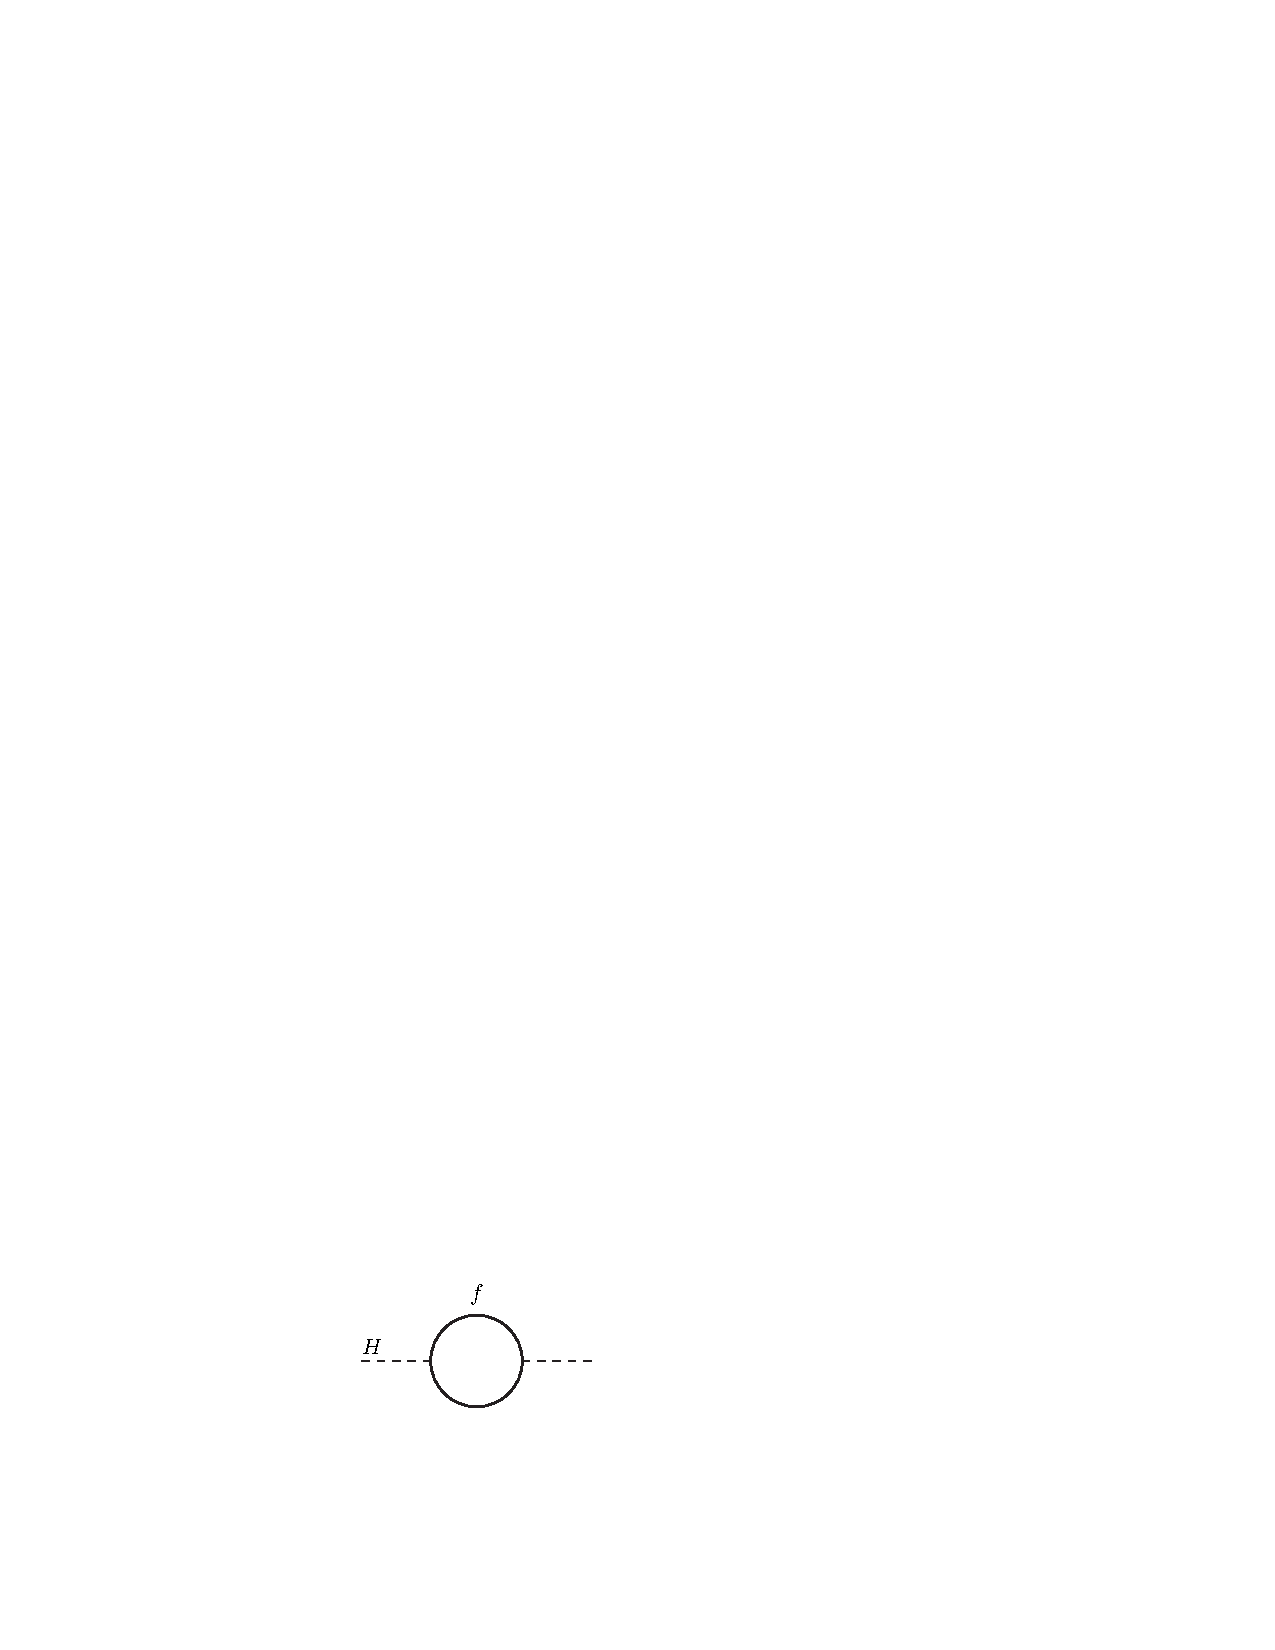
\includegraphics[width=50mm]{figures/theory/HiggsMassCorrection}
  \end{center}
  \caption{Feynman diagram for fermionic loop corrections to the mass of the Higgs boson.}
  \label{img:HiggsMassCorrection}
\end{figure}
The total contribution from these diagrams grows with the cutoff scale of the theory:
\begin{equation}
  \Delta m^{2} = \frac{|\lambda_f|^2}{8\pi^2}\Lambda_{UV}^2 ,
\end{equation}
where $\Delta m^{2}$ is the correction to the higgs mass from a massive fermion, $\lambda_f$ is the coupling constant of the higgs field to that fermion,
and $\Lambda_{UV}$ is the ultraviolet cutoff scale of the theory.
Because the top quark has the largest coupling to the higgs field of the fermions of the Standard Model,
this contribution to the mass of the higgs is dominated by loop corrections involving the top quark.
If one takes $\Lambda_{UV}$ to be the Plank mass (a natural choice for this scale),
then one would expect the Higgs mass to be 30 orders of magnitude larger than it is.
The fact that the Higgs mass is not on the order of the Plank scale is known as the hierarchy problem.
The hierarchy problem is the implication that in order for the Higgs to have a mass on the order of the electroweak scale,
the Standard Model must be extremely fine tuned, as the bare mass of the Higgs boson must be large and negative to
almost exactly cancel contributions from higher order corrections.
%implies that the Standard Model Or that the theory is fine tuned and the bare mass is large and negative almost canceling the correction''
In order to avoid having a Higgs sector that is extrordinarily finely tuned,
one can introduce new particles that also contribute to the above loop diagrams
and cancel the effect of the Standard Model fermions
or assert that the cutoff scale of the Standard Model is on the order of the Higgs Mass
(meaning, we should expect to see new physics emerge at the Electroweak Scale).
Both of these scenarios gave rise to the hope that new physical theories could be confirmed by the LHC.

A common solution to the hierarchy problem is the introduction of supersymmetric partners to the standard model fermions
that cancel out the standard model fermionic loop corrections to the higgs mass.
However, there exist many non-supersymmetric solutions to the hierarchy problem.
In particular, because the correction to the higgs mass is dominated by a top quark loop,
many of these scenarios introduce new partners to the top quark or new states that couple
strongly to the top quark~\cite{Contino:2008cx,PhysRevD.78.074026,1126-6708-2008-04-087,1126-6708-2009-05-022}.
For this reason, the top quark sector is a promising place to look for new physical signatures.
% T 5/3 and hierarchy problem:
% http://arxiv.org/abs/0801.1679v2


\subsection{Forward Backward Asymmetry}

In addition to the prospect of seeing new physical signatures at the LHC,
recent experimental results have found suggestive deviations from standard model predictions in events involving top quarks.
The validity of these deviations or the existence of models proposed to explain them are testable at the LHC.
The most promising among these results is the measurement of an excess in forward-backward asymmetry in top quark pair production events by both the CDF and D0 experiments.
These experiments both operate on the Tevatron, which is a circular $p-\overline{p}$ collider with a center-of-mass-energy of 1.8 TeV located at Fermilab outside of Chicago, Illinois.
The initial directions of the proton and anti-proton beams can be used to define forward and backward directions,
which are separated by a plane perpendicular to the beam line and going through the beam spot.
To lowest order, the pair production of top quarks is symmetric under interchange of the forward and backward regions.
At tree level in QCD, one does not expect an angular asymmetry in the pair production of top quarks.
However, at higher order, the Standard Model predicts a small forward-backward angular asymmetry that arises from QCD loop corrections \cite{Aaltonen:1318520}.
\begin{figure}
  \begin{center}
    % CDF Paper: http://arxiv.org/abs/1101.0034
    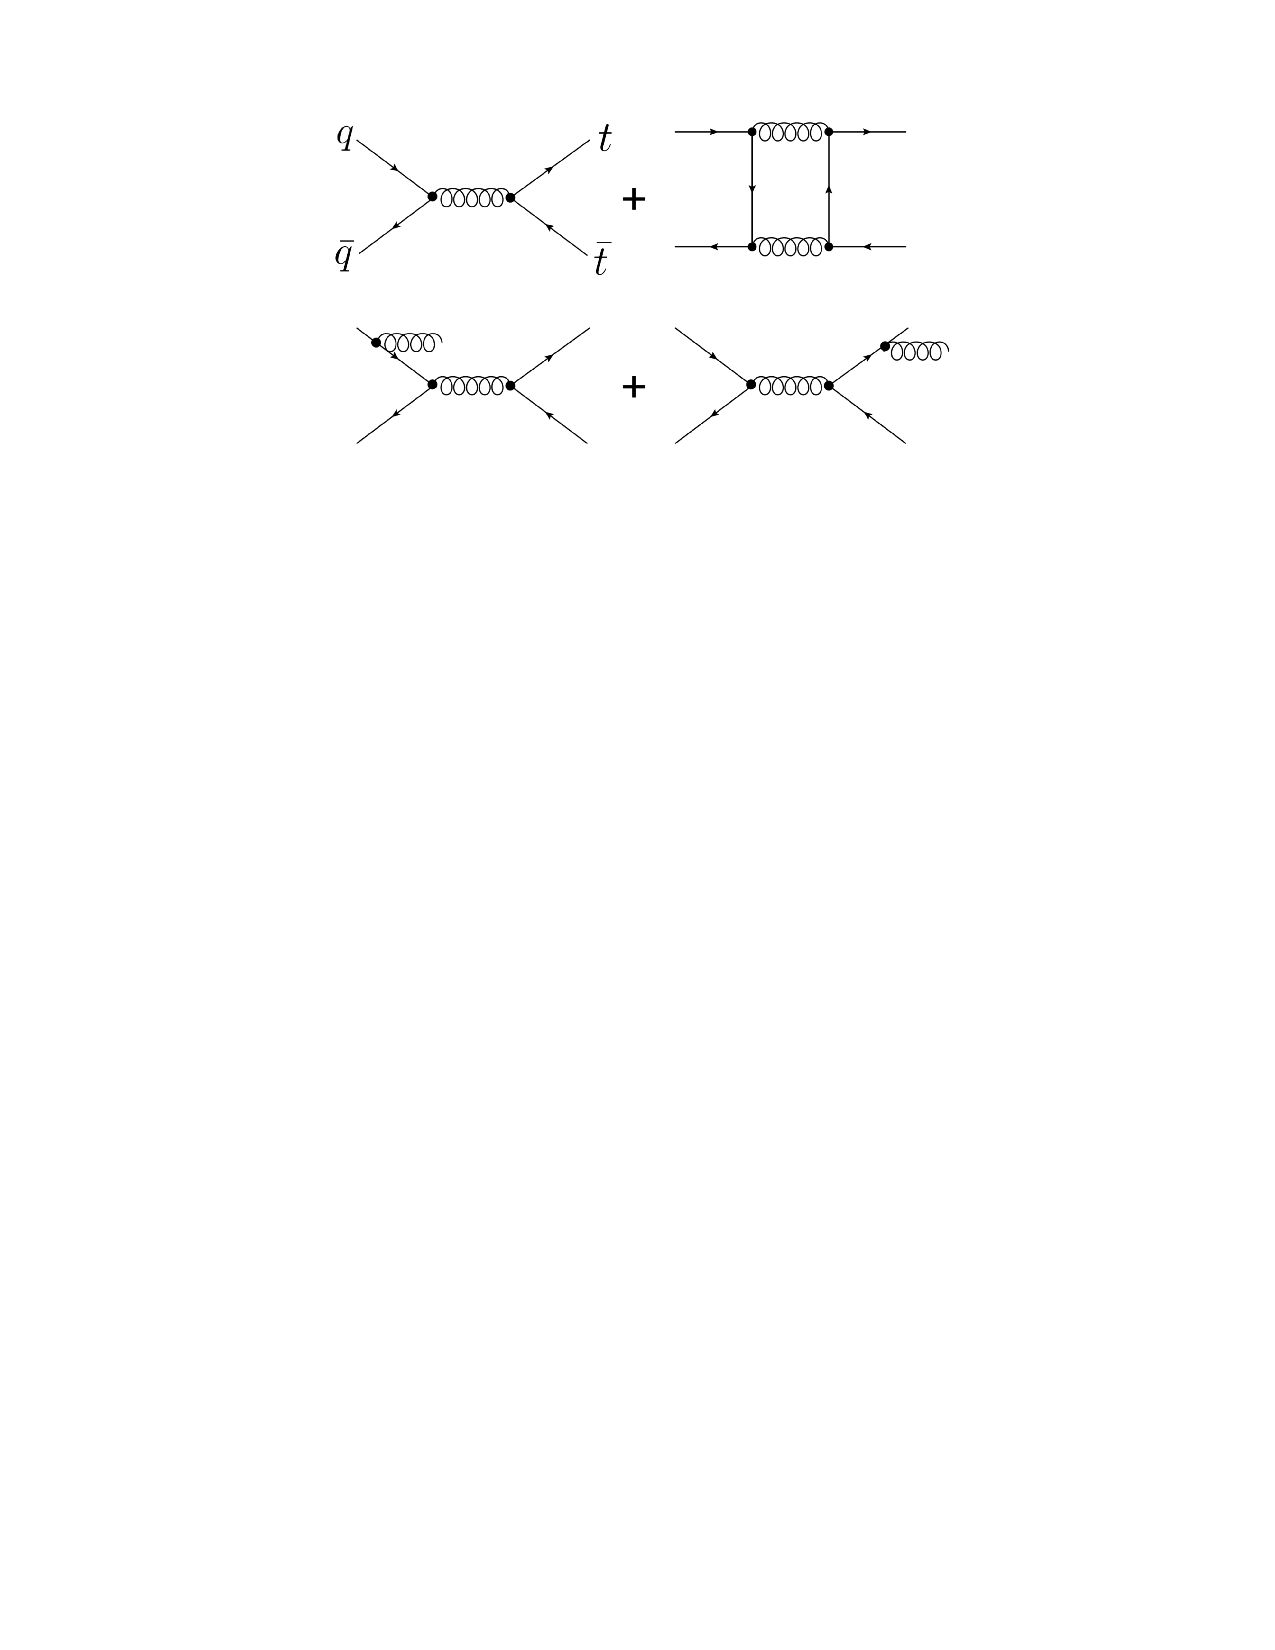
\includegraphics[width=80mm]{figures/theory/ttbarForwardBackwardFeynman}
  \end{center}
  \caption{Feynman diagrams for the pair production of $\ttbar$ in $q-\overline{q}$ collisions.  Asymmetry in the forward-background distribution of the $\ttbar$ system arises from interference between tree-level diagrams and higher-order box diagrams, as seen above.}
  \label{img:ForwardBackwardFeynman}
\end{figure}
This asymmetry can be observed experimentally using an variable that measures the directions of the top quark pairs produced at the Tevatron.
Defining the difference in rapidity between the top and anti-top quarks produced to be $\Delta y = y_{t} - y_{\ttbar}$,
one can measure the number of events with $\Delta y>0$ and $\Delta y<0$, which we refer to as $N(\Delta y>0)$ and $N(\Delta y < 0)$, respectively.
Using these definitions, one constructs the total $\ttbar$ frame asymmetry as
\begin{equation}
  \label{eq:FB_Asymmetry}
  A^{\ttbar} = \frac{N(\Delta y>0) - N(\Delta y>0)}{N(\Delta y>0) + N(\Delta y>0)}
\end{equation}
The standard model prediction for $A^{\ttbar}$ is on the order of $0.06 \pm 0.01$~\cite{Aaltonen:1318520}.
The sign of $\Delta y$ is well-defined at the Tevatron, as one can use the directions of the $p$ and $\bar{p}$ beams to 
define forward and backward regions.
However, at a $p-p$ collider, such as the LHC, the symmetry of the two incoming proton beams prevents one from consistently
defining a sign for $\Delta y$.
% http://arxiv.org/pdf/1101.0034v1.pdf

% [1] L. G. Almeida, G. F. Sterman and W. Vogelsang, Phys. Rev. D 78, 014008 (2008).
% [2] O. Antunano, J. H. Kuhn, and G. V. Rodrigo, Phys. Rev. D 77, 014003 (2008).
% [3] M. T. Bowen, S. D. Ellis, and D. Rainwater, Phys. Rev. D 73, 014008 (2006).
Both CDF and D0 measured this variable using $\ttbar$ events where one top quark decays leptonically and the other hadronically (the single-lepton decay channel).
The presence of the charged final-state lepton can be used to differentiate the top quark from the anti-top quark's decay products.
The selection of hadronic decays on the other quark results in a higher branching ratio than a selection requiring a dileptonically decaying $\ttbar$ system.

Both CDF and D0 see an enhancement in the $\ttbar$ system's forward-backward asymmetry above the small Standard Model prediction.
Of particular interest is the fact that CDF finds this enhancement to increase significantly as a function of the invariant mass of the $\ttbar$ system.
If new physics is responsible for the enhanced forward-backward asymmetry, the invariant mass dependence suggests the deviation from the Standard Model prediction may be the result of interactions with a new massive particle. % http://arxiv.org/abs/1109.3202
To explain the observations, a new particle proposed to address the Tevatron's forward-backward asymmetry must couple strongly
to both first-generation quarks and top quarks and it must couple chirally to produce an asymmetry.

Several categories of models have been proposed~\cite{Almeida:2008,Antunano:2008,Bowen:2006}.
One example is a model of composite light quarks which is enabled by a low Kaluza-Klein scale of extra dimensions~\cite{Delaunay:2011et}.  % KK Excitation: http://arxiv.org/abs/1101.2902
The compositiveness of light, right-handed quarks can lead both to a forward-backward asymmetry as well as an enhancement in the rate of high $p_T$ top quark pairs.
The asymmetry arises from the pair-production of a kk-gluon which subsequently decays into a $\ttbar$ pair, and the decay is asymmetric if there is a large difference between left-handed and right-handed bulk masses.

Other models propose a massive neutral vector boson, or simply Z', which is exchanged via the t-channel by incoming light quarks to produce outgoing top quarks~\cite{Berger:2011vi,Bhattacherjee:2011do}.
%A number of models propose %http://arxiv.org/abs/1109.3202, http://arxiv.org/abs/1102.0545v2,
This process can produce two same-sign top quarks in the final state, which is a rare signature in the Standard Model.

\begin{figure}
  \begin{center}
    % CDF Paper: http://arxiv.org/abs/1101.0034
    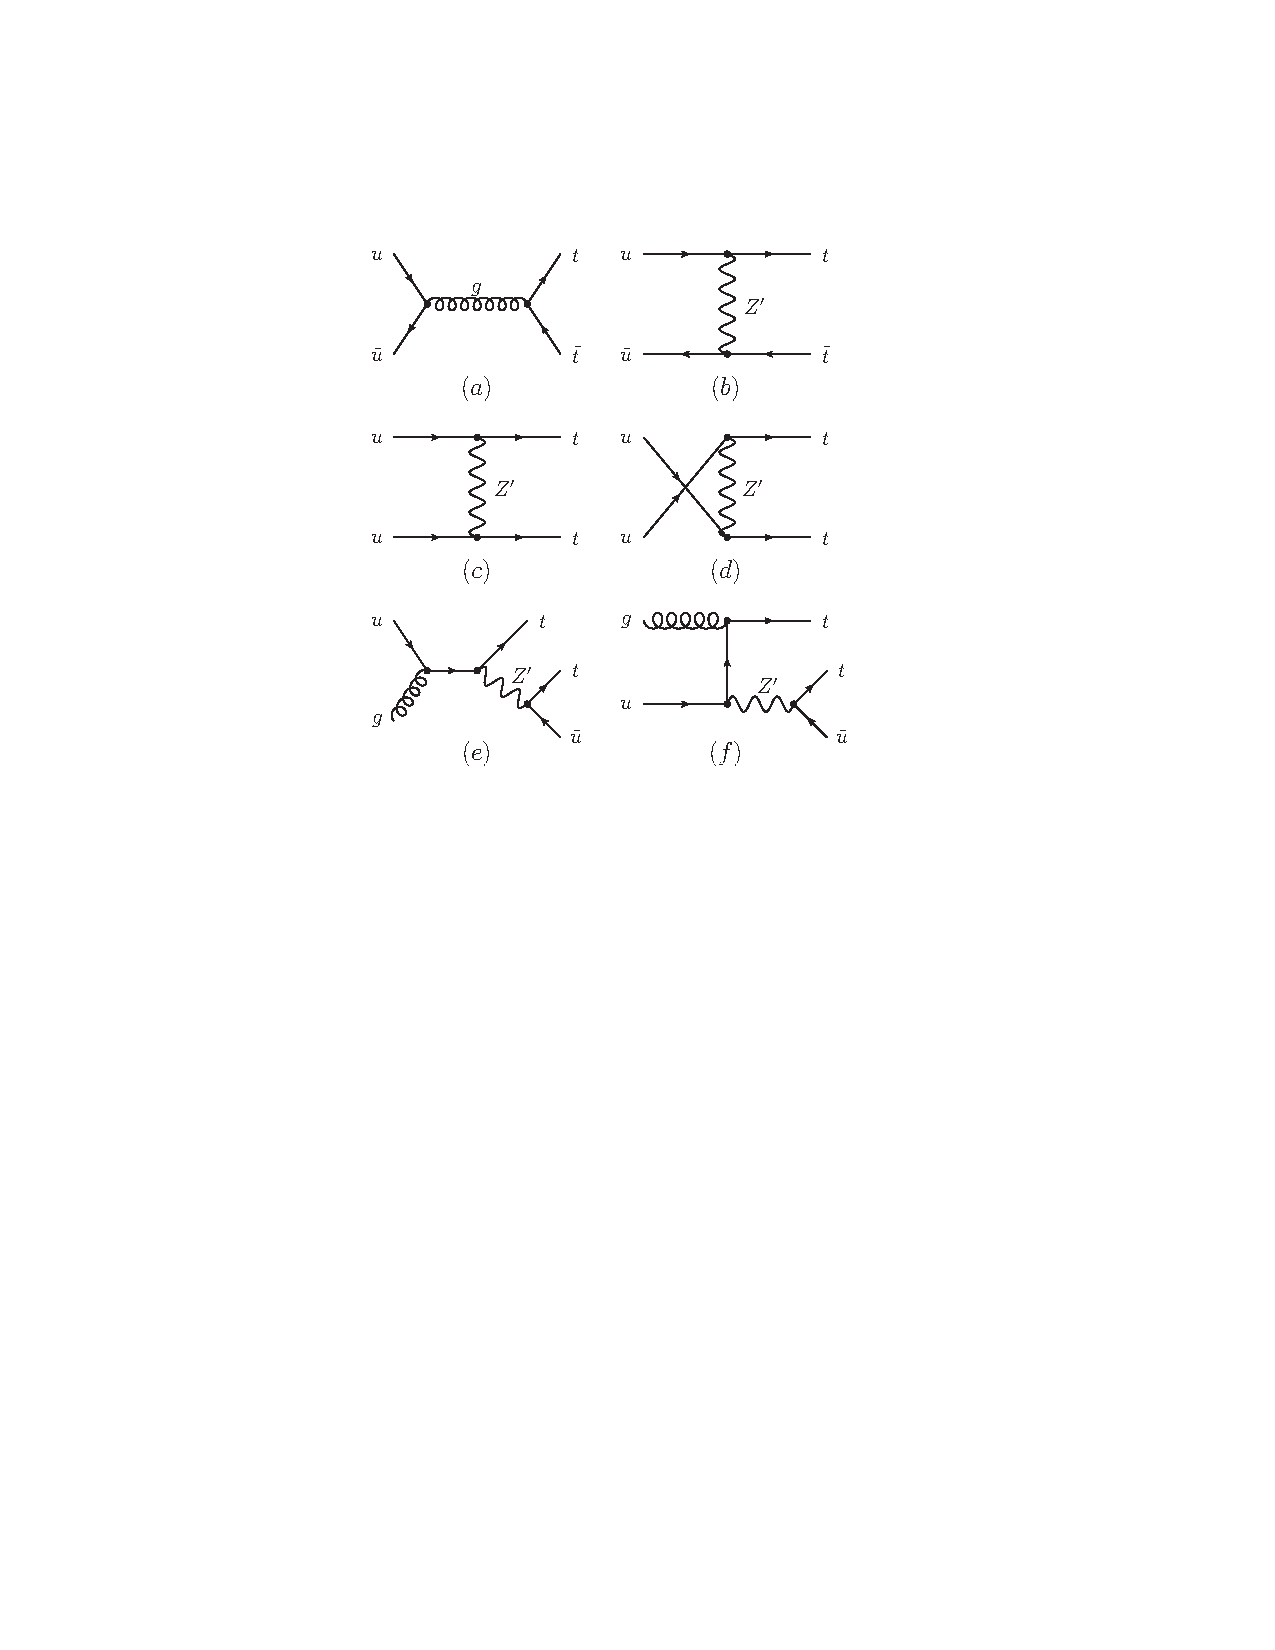
\includegraphics[width=80mm]{figures/theory/AsymmetryZPrimeModel}
  \end{center}
  \caption{Feynman diagrams of contributions to $\ttbar$ production involving a Z'.}
  \label{img:CDFAsymmetryMass}
\end{figure}

%CDF : 20.1 \pm 6.7
%D0 : 19.6 \pm 6.5 % D0 http://arxiv.org/abs/1107.4995

Because the LHC is a proton-proton collider, one cannot define a consistent forward-backward direction in the lab frame (the incoming beam is mirror-symmetric about the collision point).
%% For this reason, directly verifying the tevatron's forward-backward asymmetry anomoly at the LHC requires defining a different discriminating variable than the one used by CDF and D0.
%% Moreover, the larger gluon-gluon contribution to the top pair production cross-section increases the background rate,
%since in the Standard Model and most non-standard models explaining the forward-backward asymmetry,
%the asymmetry occurs among $\ttbar$ events with initial-state quarks. % made up: http://arxiv.org/pdf/0709.1652v1.pdf
%% One can probe this effect at the LHC by measuring a similar variable known as the charge asymmetry.
%% In this quantity, one measures $\Delta|Y| = |y_t| - |y_{\overline{t}} |$ and defines the charge asymmetry to be
%% \begin{equation}
%%   \hat{A}^{\ttbar} = \frac{N(\Delta |y|>0) - N(\Delta |y|>0)}{N(\Delta |y|>0) + N(\Delta |y|>0)}
%% \end{equation}
While this makes the direct measurement of the forward-backward asymmetry at the LHC challenging, there exist techniques for directly probing this effect using modified versions of the discriminating variable defined in equation~\ref{eq:FB_Asymmetry}.
However, equally promising is the prospect of searching for searching for models designed to explain the excess in forward-backward asymmetry observed at the Tevatron.
Several of these models require modifications to the Standard Model that are manifest in the top sector.
For this reason, searches for exotic physical models in the top sector at the LHC are a promising way to explore new physics suggested by this observed excess.
% because direct measurements of the forward-backward asymmetry as observed at the Tevatron are difficult at the LHC, indirect measurements of new physics models designed to explain the forward-backward asymmetry may be more promising.
In particular, many of these models result in same-sign top quark pairs, which can be searched for in regimes that have small backgrounds from the Standard Model, making such searches experimentally appealing.
%These indirect studies include precise measurements of the top quark pair-production cross-section and searches for excesses of events with same-sign top quark pairs.

\subsection{Precision Measurements}
An accurate understanding of the top-quark pair-production cross-section has a plethora of applications toward understanding particle physics phenomena.
Because top quarks will be produced in large numbers at the LHC, top quark decays are useful for
calibration and validation of the ATLAS detector.
Aside from the direct applications of using the top quark sector to search for new physics,
decays of top quarks are an important background to many analyses throughout analyses conducted by the ATLAS collaboration.
Because the decay of top quarks lead to a wide range of final states, they appear as backgrounds to
numerous search channels for the Higgs boson, many SuperSymmetry analyses, and across a wide range of exotic searches.

%A good example is a recent analysis which uses the \ttbar cross-section to constrian the gluon parton distribution function. % http://arxiv.org/abs/1303.7215

% However, because the The early measurements at the LHC d

%% % CDF Subsection
%% \subsection{CDF}

%% The CDF collaboration tagged $\ttbar$ events using the following event selection:
%% \begin{itemize}
%%   \item 1 selected lepton with $E_T \ge 20$ GeV and $| \eta | <$ 1
%%   \item 4 hadronic jets with $E_T  > 20$ GeV and $| \eta | <$ 2
%%   \item $\met >$ 20 GeV
%% \end{itemize}

%% The choice of jets to associate with the hadronically decaying top was made using a $\chi^2$ kinematic fit to the full $\ttbar$ system using the mass of the W-bosons and top quarks as constraints and assigning b-tagged jets, if any, to b quarks at the parton level.
%% Expected signal and background distributions were evaluated using PYTHIA Monte-Carlo simulation.

%% The CDF measurement found a forward-backward asymmetry of $A = 0.150 \pm 0.055$ (stat+sys), which is two standard deviations away from the predicted value from NLO simulations.
%% In addition, the significance of this deviation was examined as a function of both the difference in rapidity ($Y$) and the invariant mass of the $\ttbar$ system:

%% % From Here: http://arxiv.org/pdf/1101.0034v1.pdf
%% % Page 13: http://arxiv.org/abs/1101.0034
%% \begin{tabular}{lcc}
%% Selection                         &   CDF Result    & SM Prediction \\
%% $A^{\ttbar}_{FB}( \Delta Y < 1.0)$  & 0.026 $\pm$ 0.118 & 0.039 $\pm$ 0.006 \\
%% $A^{\ttbar}_{FB}( \Delta Y > 1.0)$  & 0.611 $\pm$ 0.256 & 0.123 $\pm$ 0.008 \\
%% \hline
%% $A^{\ttbar}_{FB}( M_{\ttbar} < 450 GeV)$   & -0.116 $\pm$ 0.153 & 0.040 $\pm$ 0.006 \\
%% $A^{\ttbar}_{FB}( M_{\ttbar} \ge 450 GeV)$ & 0.475 $\pm$ 0.114  & 0.088 $\pm$ 0.013 \\
%% \hline
%% \end{tabular}

%% Of note is the fact that the deviance of the asymmetry from prediction is a function of the invariant mass of the $\ttbar$ system.

%% \begin{figure}
%%   \begin{center}
%%     % CDF Paper: http://arxiv.org/abs/1101.0034
%%     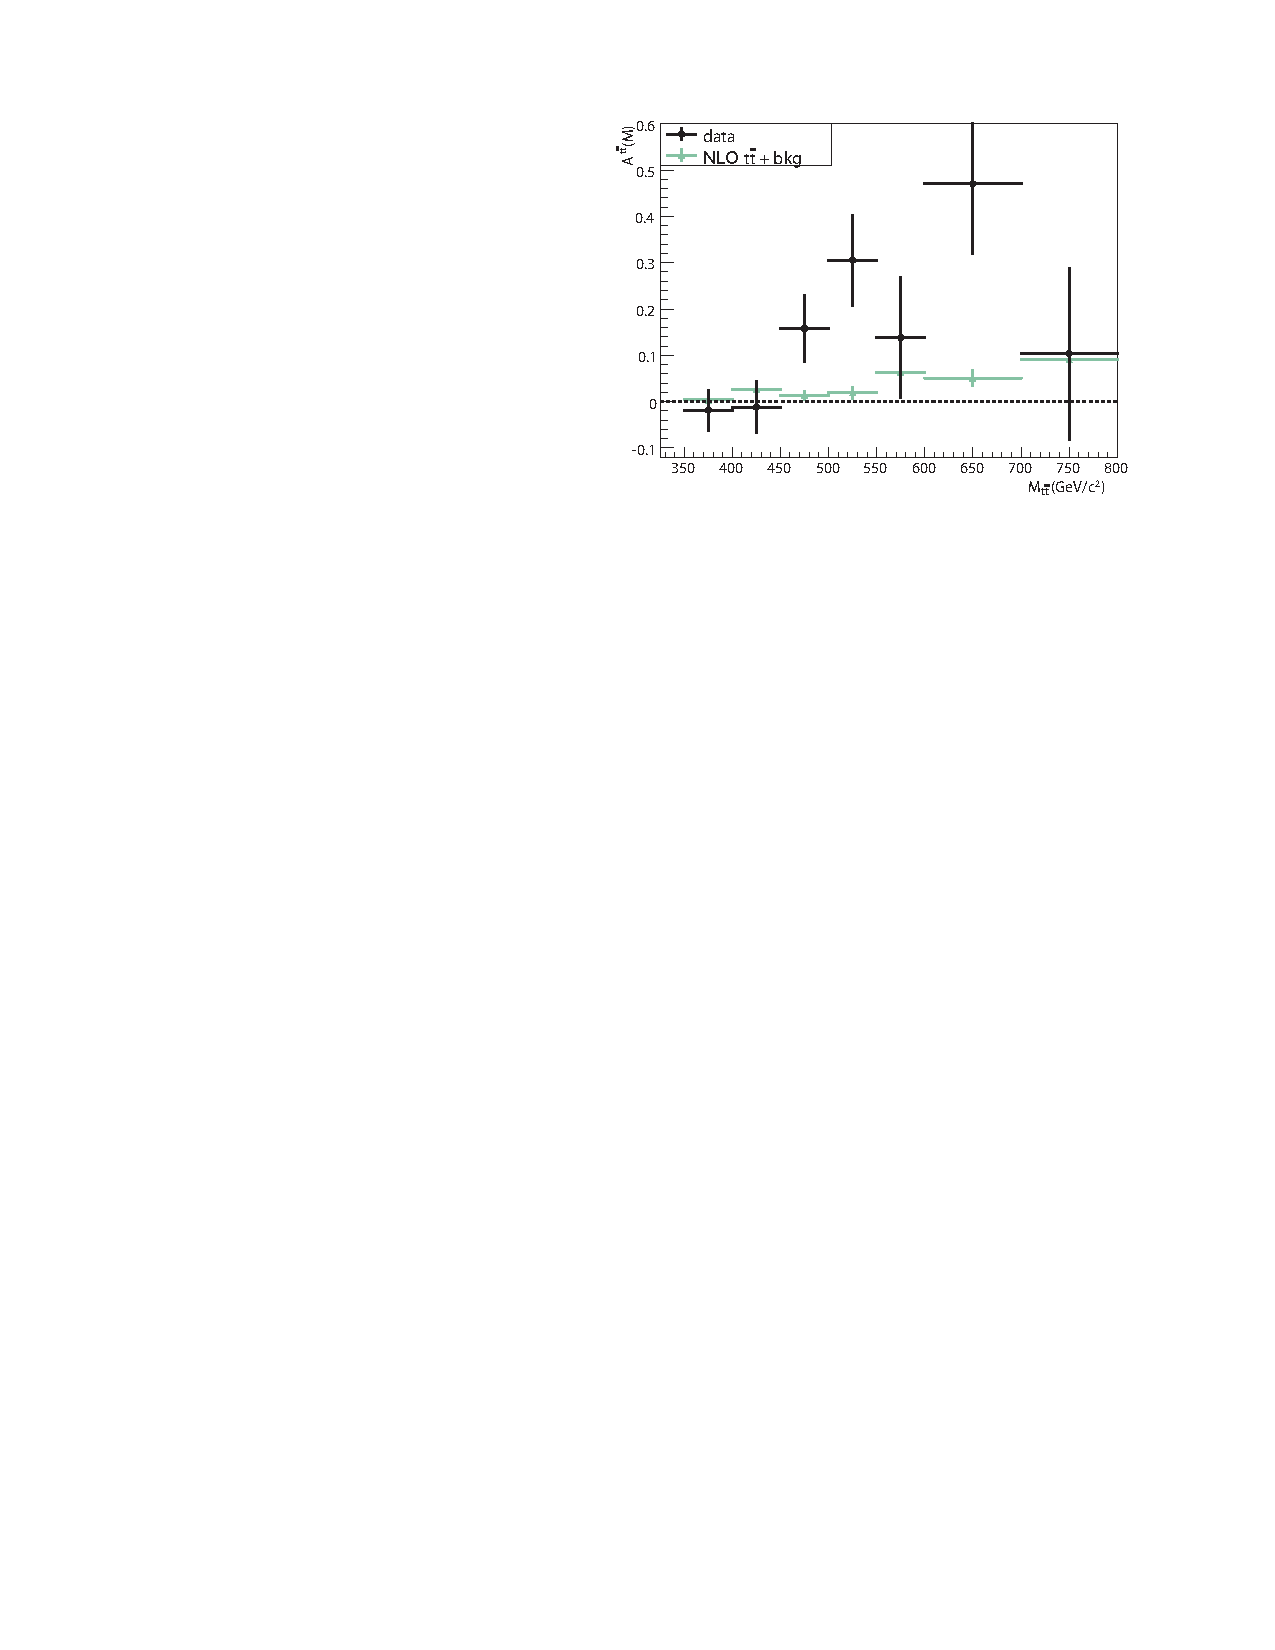
\includegraphics[width=80mm]{figures/theory/CDFAsymmetryMass}
%%   \end{center}
%%   \caption{Graph of the forward-backward asymmetry as a function of the invariant mass of the $\ttbar$ system.}
%%   \label{img:CDFAsymmetryMass}
%% \end{figure}


%% % D0 Subsection
%% \subsection{D0}

%% The D0 experiment selected $\ttbar$ events by triggering on either a lepton or a lepton+jet and further requiring
%% \begin{itemize}
%%   \item An isolated lepton with $p_T >$ 20 GeV and $|\eta| <$ 1.1 for electrons or $|\eta| <$ 2.0 for muons
%%   \item $\met >$ 20 GeV for electron events or $20 GeV < \met < 250 GeV$ for muon events
%%   \item $\Delta \phi(e, \met) > (2.2 - 0.045*\met / GeV)$ radians for electron events or $(p_T^\mu + \met)^2 - (p_x^\mu + \met_x)^2 - (p_y^\mu + \met_y)^2 < (250 GeV)^2$
%%   \item 4 jets, each with $pt > 20 GeV$ and $|\eta < 2.5|$ where the leading jet has $p_t > 40 GeV$
%% \end{itemize}

%% D0 measured an overall forward-backward asymmetry of $(9.2 \pm 3.7)$\%, where the predicted value is $(2.4 \pm 0.7)$ \%.

%% \begin{tabular}{lcc}
%% \hline
%% Selection                         &   CDF Result    & SM Prediction \\
%% \hline
%% $A^{\ttbar}_{FB}( \Delta Y < 1.0)$ &   6.1 $\pm$ 4.1 & 1.4 $\pm$ 0.6 \\
%% $A^{\ttbar}_{FB}( \Delta Y > 1.0)$ &  21.3 $\pm$ 9.7 & 6.3 $\pm$ 1.6 \\
%% \hline
%% $A^{\ttbar}_{FB}( M_{\ttbar} < 450 GeV)$ & 7.8 $\pm$ 4.8 & 1.3 $\pm$ 0.6 \\
%% $A^{\ttbar}_{FB}( M_{\ttbar} \ge 450 GeV)$ & 11.5 $\pm$ 6.0 & 4.3 $\pm$ 1.3 \\
%% \hline
%% \end{tabular}

%\subsection{Discussion}

% LocalWords:  Higgs

\clearpage
\newpage

%
%
%

\section{ATLAS}
ATLAS is a multi-purpose particle detector designed for particle discovery.
In order to fulfull this broad role, ATLAS must excel in several ways:

\begin{itemize}
  \item It must be sensitive to a wide spectrum of particle that can be produced by particle colissions, including Leptons (Electrons and Muons), Hadrons (Pions, Kaons, and the many other bound states of quarks that typically come in the form of Jets), and Photons.
  \item It must be able to identify precisely the kinematic properties of these particles, which includes measuring their energies and directions with a high resolution.
  \item It must maintain its resolution over a large range of energies, roughly from 1 GeV up to and including the TeV scale.
  \item It must make these measurements at an extremely high rate, millions of times a second, and over the entire lifetime of the experiment, which could end up being decades
  \item It must be able to record, save, and successfully distribute its collected data to experimentalists and analyzers around the world.
\end{itemize}

These requirements are entirely non-trivial, and fulfilling them required decades of design, construction, engieneering, and maintenence.  
The original design for ATLAS
In order to be successful, ATLAS 
to use a wide spectrum of detector designed to discover particles and to precisely measure their proproperties.


Typical descriptions of the ATLAS detector list its various components and describe their properties.
But perhaps it is more useful to instead approach the detector from the perspective of the different particles that it is designed to detecct, and to use that as a springboard to go into machine's enieneering details.

\subsection{Layout and Geometry}
Cylander, eta, phi size, underground, lhc, geneva, Mount Blanc, etc


\subsection{Overview}
ATLAS is a multi-component detector consisting of many individual subsystems, each of which measures a certain number of kinematic properties of particles created or scattered by the LHC.
Only when combining the measurements of these sub-systems do complete pictures of particles and entire begin to emerge.
The subcomponents of ATLAS are layered around the central location of the primary interaction.
The inner-most layer of ATLAS is the ``inner detector'', which consists of silicon strips and pixils and is designed to track the 3-d trajectories of charged particles passing through it.
The inner detector extends for 1.15 m and is surronded by a solonodial magent which provides a 2T field within the inner detector.
This field causes charged particles to bend and allows the inner detector to measure the momenta of charged particles by fitting their trajectories.
Surronding the inner detector is the electromagnetic calorimeter, which consists of alternating layers of lead absorbers and active electronics that are baithed in liquid argon.
The liquid argon must of course remain cooled, and so the electromagnetic calorimeter is located within a cryostat that maintains a temperature of [XX].
To reduce the amount of upstream material present before the calorimeter systems, the solonodial magent for the inner detector is located within the EM calorimeter's cryostat.
A dedicated presampler is located directly behind the cryostat's wall to correct for any energy lost within inactive material in front of the EM calorimeter.
Behind the outside of the cyrostat and past the EM calorimeter is the hadronic calorimeter, which consists of alternating layers of iron and scintillating tile.
Finally, the outer-most layer of ATLAS is the muon spectrometer, which consists of many subsystems designed to detect the trajectories of muons at high rates and with good resolution. 
A 8T magnetic field is induced across the entire muon system and is produced by large superconducting toroid magnets.

\subsection{Inner Detector}
The inner detector is first part of the ATLAS detector encountered by particles emerging from the interaction point.
The inner detector (ID) consists of three subsystems which are designed to track the trajectories of charged particles as a collection of discrete points where they hit active parts of the detector.

The first layer of the ID is the pixel detector, which itself consists of three barrel layers of pixel modules at radaii of 4 cm, 10 cm, and 13 cm (on average) as well as five disks on each side of the deterctor to cover the forward region in pseudorapidity.
Each region contains a collection of pixel modules (which are identical across the barrel and disk regions) which are 62.4 mm long and 21.4 mm wide.
The individual modules contain 61,440 pixel elements, and there are 1500 such modules in the barrel and 700 in the disks. %read out by 16 chips, each serving an array of 24 by 160 pixels 
In total, there are about 140 million detector elements. % each 50 μm in the Rφ direction and 300 μm in z,
The pixel detectors are designed to measure the impact parameters of short-lived particles lead to non-neglegable displaced vertices, such as $\tau$s and b-quarks.
% Pixel Image: http://www.atlas.ch/pixel-detector.html
% Paper and individual pixel image: http://arxiv.org/pdf/physics/0412138.pdf

Moving outward through the inner detector, the next layer encountered is the Semiconductor tracker (SCT).
Since it exists at a larger radius, the SCT must cover a larger area (about 61 $m^2)$ with active material.
The detector contains 6.2 million readout channels that are spread across four complete barrels at radii of 30.0, 37.3, 44.7 and 52.0 cm, and three rings of end-cap detectors on either side.
Each subdetector consists of a collection of 6.36$\times$6.40 $cm^2$ silicon strips (each with 768 readout strips) arranged in an overlapping pattern with each strip aligned at a small angle.
The spatial resolution is of the SCT is 16 $\mu$m in $R-\phi$ and 580 $\mu$m in z, which can distinguish tracks that are separated by as little as 200 $\mu$m.

The final component of ATLAS' inner detector is the Transition Radiation Tracker (TRT).

\subsection{Electromagnetic Calorimeter}
The subcomponents that make up ATLAS's electromagnetic calorimeter are each designed to measure the energy of electrons and photons by inducing and absorbing an elecromagnetic shower.
Heavier charged particles, such as muons and pions, will interact with electromagnetic calorimeters, but their interaction lengths are longer than those of electrons and photons, which makes their showers more elongated.
As a result they do not deposit a majority of their energy within the range of ATLAS' EM calrimeters.
ATLAS' Electromagnetic calorimeter is divided into three subsections consisting of the barrel calorimeter, which covers a pseudorapidity range of $|\eta| < 1.475$ and the two end-cap calorimeters, which covers $1.375 < |\eta| < 2.5$.
However, as opposed to the hadronic calorimeter, each subcomponent shares a common design.
The calorimeter consists of layers of lead absorbers shaped in a zig-zag, accordian-like pattern and similarly arranged Kapton electrodes placed in the middle of gaps between the lead absorbers.
%The calorimeter consists of alternating layers of Kapton electrodes and lead absorbers that are both shaped in a zig-zag, accordian-like pattern.
The calorimeter's zigs and zags are aligned in the radial direction, which removes the possability of inactive cracks where two plates meet.
The entire calorimeter is bathed in liquid argon, which is maintained at a temperature of about 88 degrees kelvin by the cryostats that encases the electromagnetic calorimeters (for this reason, ATLAS' electromagnetic calorimeters are commonly referred to simply as the ``LAr calorimeter'').
As charged particles fly through the calorimeter, they will ionize the Liquid Argon, and ionized electrons are drawn toward the active electrodes by a high voltage electric field (of about 1 kV/mm) that is maintained throughout the calorimeter. % [http://arxiv.org/pdf/0912.2642v4.pdf]
The current absorbed is preportional to the energy deposited, which is used to reconstruct the energy of the electron hitting the calorimeter.
Each LAr calorimeter is segmented into three or four transverse layers and is divided into cells of varying granularity in  $\Delta \eta \times \Delta \phi$, depending on the location and on the layer.%$ = 0.1 \times 0.1$ for $|\eta| < 2.5$ and up to $\Delta \eta \times \Delta \phi = 0.4 \times 0.4$. for $3.1 < |\eta| < 4.9$.
In all, the LAr calorimeter has 182,468 readout cells.
Of particular importance is the first layer of very LAr barrel calorimeter, which is finely segmented ``strips'' of  $\Delta \eta \times \Delta \phi = (0.0031 \times 0.098)$. 
This this $\eta$ segmentation allows for the resolution of the EM shower shape differences between photons and $\pi_{0}$s which decay into narrowly separated photon pairs, 
In the barrel, the three layers of LAr calorimeters have thicknesses of 4.3, 16, and 2 radiation lengths, respectively.
In addition, the barrel contains a presampler layer, which consists of LAr electrods, but no lead absorber, that is used to correct for energy lost in the inner detector, the solenoid magnet, and in the cryostat walls (the end caps have less material upstream from the EM calorimeters and therefore don't require a presampler). % [http://www.hep.lu.se/atlas/thesis/egede/thesis-node43.html]

% Helpful Talk: [http://www.physics.utoronto.ca/~krieger/talks/Krieger_NSS05_Talk.pdf]
% Commissioning ATLAS paper: [http://arxiv.org/pdf/0912.2642v4.pdf]
% LAR Temperature: [http://cdsweb.cern.ch/record/686091]


\subsection{Hadronic Calorimeter}
The Large Hadron Collider is thus named because it collides a specific hadronic bound state of quarks known as the proton.
The majority of interactions between these particles are mediated by the strong force (QCD), and the vast majority of final state particles are cone-like sprays of hadronic particles known as Jets.
It is therefore crucial that a detector working with a hadron collider be excellent at identifying and measuring hadronic particles.

% General Hadronic Calo layout
The primary means of studying a jet is through calrimetry, where the energy of a jet is determined by stopping its hadronic shower using a dense material and measuring the energy it deposits in an active material.
The direction of the jet is determined by the  $\eta$, $\phi$ location of where the jet hits the detector.
The ATLAS hadronic calorimeter is designed to contain as much of a hadronic shower within the calorimeter itself and to accurately determine its energy using the calorimeter's active components.
It is divided into three subsystems that cover overlapping ranges in pseudorapidity.
The largest and most important is the ``tile'' hadronic calorimeter (which itself is divided into the ``barrel'' and two ``extended barrel'' tile calorimeters), which covers the rapidity region of $|\eta| < 1.7$. [tdr]  
The ``hadronic end cap'' (HEC) extends the calorimeter's range up to $|\eta| < 3.2$, and the ``forward calorimeter'' (FCAL) covers the pseudorapidity range of $3.1 < |\eta| < 4.9$.  
%Each of these subsystems have similar goals but vary in their design.

% [pdg review: http://pdg.lbl.gov/2011/reviews/rpp2011-rev-passage-particles-matter.pdf]

% [http://rd11.web.cern.ch/RD11/rkb/PH14pp/node80.html]

% The Tile
The hadronic tile calorimeter, which covers [XX] starradians, detects jets that emerge low pseudorapidity, including those that are close to perpendicular to the beam pipe.
It is a cylindric shell ranging from an inner radius 2.28 meters and outer radius 4.25 meters.
The tile is made of three subsystems, one central ``barrel'' calorimeter which covers $|\eta| < 1.0$ and two ``extended barrel'' calorimeters, which cover $0.8 < |\eta| < 1.7$ on either side.
The tile calorimeters consist of alternating layers of 14 mm iron plates, which is used for inducing the hadronic shower and stopping the jet, and 3mm active scintillating-tile, which is used to measure the energy deposited into the calorimeter by the jet.
%Iron is used because the hadronic particles that make up jets interact strongly with nucleii, and therefore a material with a high nuclear density is desirable.
The scintillating tile is attached to a series of photomultiplier tubes (PMTs) that amplify the tile's electrical readout.
Key to the successful performance of the tile calorimeter is providing enough average interaction lengths for the hadronic shower to be contained.
The hadronic thickness at the end of the tile calorimeter (at $\eta=0$) is 9.2 $\lambda$, which is enough to ensure good jet resolution and to minimize jet ``punch through'' into the muon system.



\subsection{Muon Spectrometer}

\subsection{Measuring Particles with ATLAS}

\subsection{Jets}
Jets are produced when particles with color charge, quarks and gluons, are in the outgoing states of a hard interaction.
As these particles propogate through space, they will tend to decay into or radiate other color-charged particles, leading to a phenomenon known as the evolution of a ``parton shower.''
This shower grows rapidly because QCD, which is an asymptotically free field theory, has a small coupling constant at high energies.  
As the shower progresses and the average energy of the constituent particles decreases, the QCD coupling constant will grow stronger, and this will cause the quarks and gluons to bind together into stable particles in a process known as ``hadronization.''
The collection of these hadrons, which move in a wide, cone-like shape, is known as a jet.
%The average distance for the parton-shower, hadronization evolution process is small compared to the radius of ATLAS, adn so jets are fully formed as they begin to interact with the detector

A jet originating from the beam spot and and moving through ATLAS will first interact with the inner detector.  Since many of the constituent particles of a jet are charged hadrons ($\pi^{+}$, $K^{+}$, etc), they will leave tracks in the ID.
Jet algorithms can use these tracks when attempting to identify a jet, and there are algorithms that exclusively rely on this collection of tracks to build a set of identified jets (

%[ Track Jets, 2009: https://atlas.web.cern.ch/Atlas/GROUPS/PHYSICS/CONFNOTES/ATLAS-CONF-2010-002 ].

However, the most common way to reconstruct jets is using the calrimetry.
Jets will deposit a small fraction of their energy in the Electromagnetic Calorimeter, but the majority of the shower's energy is measued by the hadronic calorimeter.
There are many algorithms used to reconstruct jets using information from the hadronic calorimeter, but most of them consist of clustering algorithms which group together cells of energy deposits.
The main differences between techniques involve how these energy deposits are calibrated (if at all) and how the cells are clustered (based on fixed geometries, such as cones, or based on iterative algorithms using a distance function to merge cell deposits).
A small number of jets managed to escape the hadronic calorimeter and enter the muon chambers, where they can be misidentified as mouns.
In addition, jets with ``heavy flavor'' may contain decays that result in real muons (but not muons that originated from a hard collission in the beam spot), so care must be taken to separate muons originating as jets from muons originating from the hard process.

% How jets work, and how they shower

%% The first step in measuring a jet's energy is stopping it.  
%% The hadronic partilces that make up a jet are made up of quarks and gluons, which are charged under the strong force (QCD).
%% They therefore interact with the nucleii of materials that they pass through.
%% The primary mechanism for energy loss of high energy hadrons traveling through a solid material is via inelastic nuclear interactions.
%% As these interactions cause the original hadron to lose energy, they will also cause nuclear excitations and subsequent nuclear decays in the material.
%% This in turn leads to the emission of additional hadronic particles, which themselves will interact with the material.
%% The net effect is the formation of what is known as a hadronic shower.
%% When the energy of the daughter particles in the shower becomes too small for nuclear excitation, the shower ceases to evolve, and the remaining energy of hadrons is lost to ionization and electromagnetic interactions.
%% While the majority of energy is lost via nuclear interactions, a non-neglegable fraction of a jet's energy interacts electromagnetically .
%% This fraction 


\subsection{Electrons}
Electrons and positrons are electromagnetically charge and wil therefore interact with the innner detector, and in addition their trajectories will be curved as the particles are beant by the magnetic field.
As they pass through the inner detector, electrons will deposit hits in the pixles, silicon, and straw tubes, and the collection of these hits can be extrapolated together to reconstruct the electron's track.
This track is of crucial importance for identifying electrons.
The track carries information both about the direction of the electron, but also about its momentum, and the presence of a track is necessary to distinuish electrons from photons, which lead essentially identical electromagnetic showers in the EM calorimeter.
When electrons enter the EM calorimeter, they will begin to decellerate, which will cause the electron to radiate via bremsstralung.
The radiated photons often have enough energy to produce electorn-positron pairs, which themselves will emit bremsstralung radiation.
This creates a cascade of electrons, positrons, and photons that is collectively known as an electromagnetic shower.
The energy of this shower is determined as it is absorbed by the EM calorimeter.
The EM calorimeter tends to provide a better energy resoltion for high pT electrons than the tracks do (beginning when the electron's energy is around 10 GeV).

% [ 2010 performance: http://cdsweb.cern.ch/record/1273197 ]
% [ https://atlas.web.cern.ch/Atlas/GROUPS/PHYSICS/PUBNOTES/ATL-PHYS-PUB-2011-006/ATL-PHYS-PUB-2011-006.pdf ]
% [ Moriond 2012 Resolution info: https://indico.cern.ch/getFile.py/access?contribId=3&resId=1&materialId=slides&confId=163471]
% [ https://twiki.cern.ch/twiki/pub/AtlasProtected/EnergyScaleResolutionRecommendations/summary_rel16.pdf ]

\subsection{Photons}
Photons are identified as electromagnetic showers that aren't matched to an inner detector track.
In addition, photons may decay into an electron-positron pair before entering the EM calorimeter.
If this occurs within or before the inner-detector, the proximity of the electron and positron's tracks can be used to identify the pair as a photon that ``converted'' electromagnetically, and the pair can be reconstructed as a single photon.
%In addition, photons may be identified as electron-positron pairs  from ``conversions,'' which are electron-positron pairs that 


\subsection{Muons}
Muons, with a mass of 106 MeV, weigh about 200 times more than the electron (which weights .512 MeV).
This implies that, for a fixed energy, a muon will have a smaller value of $\beta$ than an electron (or, equivalantly $\gamma$), which results in a smaller amount of radiation being emitted as it passes through matter.
Therefore, a muon's mean radiation length in ATLAS' calorimeters will be much longer than an electron's length, and a significant EM shower will not develop within the detector.
For this reason, most of a muon's energy escapes ATLAS.  

% [ pdg: Muons through matter: http://pdg.lbl.gov/2000/passagerpp.pdf fig 23.1 ]

Since one can not measure its energy through calrimetry, ATLAS instead measures its momentum by estimating its curvature when bent in a magnetic field.
A Muon will create a bent track in the inner detector that can be used to estimate its momentum.
However, the resolution of the inner detector for high pt muons becomes somewhat poor.
To vastly improve on the measurement of the inner detector alone, ATLAS has a large set of detectors that comprise the muon spectrometer.

\clearpage
\newpage

% Chapter 2
%
%
%

\section{Top Quark Pair-Production Cross-Section Combination}

A precise measurement of the Top Quark Pair-Production Cross-Section is crucial for understanding the performance of the ATLAS detector, for testing predictions of the standard model, to searching for or constraining many new physical models.
In particle physics, a cross-section is a way to describe the rate of a specific interaction or class of interactions independently of beam conditions that are used to produce it.
The value of the top-quark pair-production cross-section in the Standard Model can be predicted using Monte-Carlo simulation techniques \cite{TOP_XSC_THEORY} \cite{TTBAR_HADRON_COLLIDERS} \cite{THRESHOLD_EXPANSION_XSC}.
This value can be determined using ``Next to Leading Order'' techniques (NLO) and is corrected by adding the ``Next to Next to Leading Order'' soft logarithm terms (approximate NNLO).
This value is determined to be $\sigma_{\ttbar} = 165^{11}_{16}$ with an uncertainty below 10\%.
The most accurate experimental determinations of the top quark's cross section previous to the LHC's results were measured by the CDS and the D0 collaborations at the Tevatron \cite{TEVATRON_XSC_LJETS} \cite{TEVATRON_XSC_DILEP}.
These experiments determined the cross-section at a center-of-mass energy of $\sqrt{s} = 7 TeV$ to a precision of 8\% using individual channels and 6.4\% by combining measurements across multiple channels.

The top-quark pair-production cross section has been measured at ATLAS using many channels and analysis technqiues.
The most precise measurements use combination of several individual measurements, which reduces both statistical and systematic uncertainties.
This section presents an ATLAS measurement of the $\ttbar$ cross-section that statistically combined three separate analysies strategies.
The likelihoods for measurements using single-lepton, dilepton, and all-hadronic channels were modeled as functions of the top cross-section, as well as a variety of nuisance parameters.
% This combination was performed by modeling the likelihoods of several individual measuremnets as functions of the top cross-section as well as a variety of nuisance parameters.
These likelihoods were then merged and a simultaneous fit to the measured data across all channels was performed.

The combined measurement of the $\ttbar$ cross-section used a measurement in the lepton+jets channel which was performed using 0.7$\ifb$ of data recorded in 2011 \cite{LEPTON_JETS_NOTE_2011}, a measurement in the dilepton channel which was performed using XX, and a measurement in the all-hadronic channel, which was performed using XX.


\subsection{Top Quark Pair-Production}

The primary means of producing top quarks at the LHC is via gluon fusion and subsequent decay into a pair of top quarks.

\begin{figure}
  \begin{center}

    \subfigure[Production]{
      % TopQuarkPairProductionDiagram: http://kjende.web.cern.ch/kjende/netzwerk/images/Feynman/WplusWminusBBar.png
      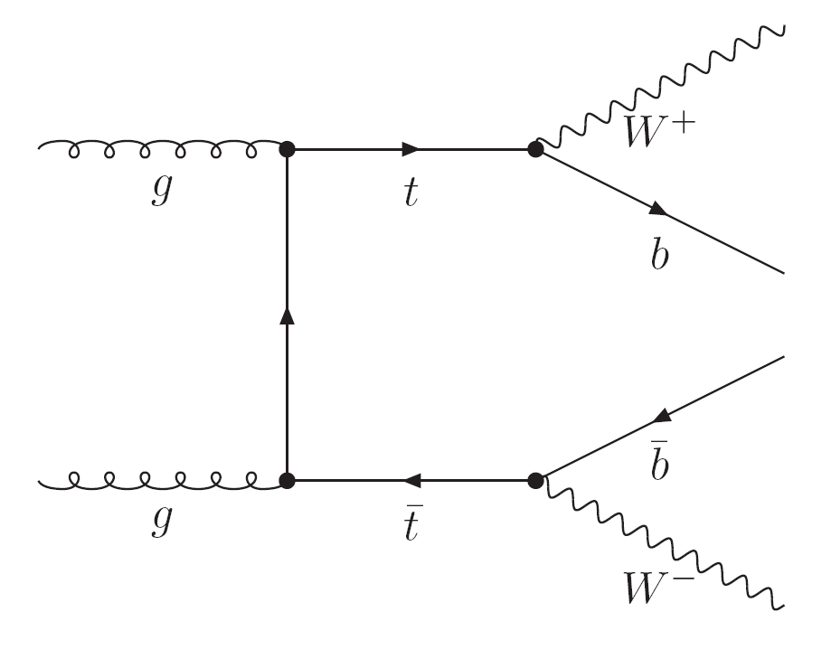
\includegraphics[width=.4\linewidth]{figures/xsection/TopQuarkPairProductionDiagram.png}
    }
    \subfigure[Decay]{
      % TopQuarkBranchingRatios: http://ej.iop.org/images/0034-4885/75/5/056201/Full/rpp347183f06_online.jpg
      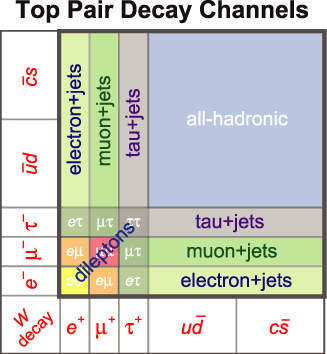
\includegraphics[width=.4\linewidth]{figures/xsection/TopQuarkBranchingRatios.jpg}
    }
  \end{center}
  \caption{ A typical feynman diagram of top quark pair production at the LHC.  Top quarks decay into W-bosons and b-quarks nearly 100\% of the time.  The subsequent decays of the W-Bosons determine the event topology of the \ttbar event.  Diagram showing the branching ratios of Top Quark pairs into leptons and quarks.}
  \label{img:TopQuarkPairProduction}
\end{figure}

W bosons decay either leptonically, in which they produce a lepton and a neutrino, or hadronically, in which they produce a pair of quarks.
W's decay leptonically XX\% of the time, which consists of decaying via $W- \rightarrow e \bar{\nu_{e}}$ 10.75\% of the time, via $W- \rightarrow \mu \bar{\nu_{\mu}}$ 10.57\% of the time, and via $W- \rightarrow \tau \bar{\nu_{\tau}}$ 11.25\% of the time, and decay into quarks the other 67.60\% of the time. % [pdg]
% W-Boson: http://pdg.lbl.gov/2012/listings/rpp2012-list-w-boson.pdf
However, tau leptons are themselves unstable particles that subsequently decay either leptonically (muon 17.41 or electron 17.83), or hadronically 64.76\% of the time, with about 50\% of the tau's today decays into 1 hadron and 15\% into 3 hadrons.
% Tau pdg: http://pdg.web.cern.ch/pdg/2012/listings/rpp2012-list-tau.pdf
In the discussion that follows, we will consider the $W \rightarrow \tau  \rightarrow e$ or $W \rightarrow \tau  \rightarrow \mu$ to be leptonic decays of the top, and we will ignore the intermediate state $\tau$ in terms of our classification.
Hence, a pair of top quarks, which we assume always decay into a pair of W bosons, will decay into two leptons 6.5\% of the time (known as the ``dilepton'' channel), into a single lepton and a pair of quarks 34.4\% of the time (known as the ``single lepton'' channel), and entirely into quarks 45.7\% of the time (known as the ``all hadronic'' channel).
% pdg:
% Citation: J. Beringer et al. (Particle Data Group), PR D86, 010001 (2012) (URL: http://pdg.lbl.gov)



%% \begin{figure}
%%   \begin{center}
%%     % TopQuarkBranchingRatios: http://ej.iop.org/images/0034-4885/75/5/056201/Full/rpp347183f06_online.jpg
%%     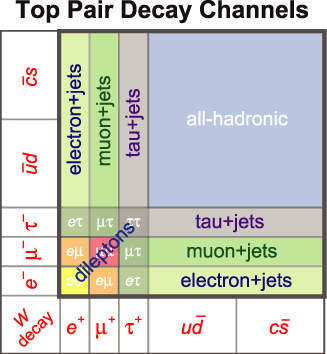
\includegraphics[width=100mm]{figures/xsection/TopQuarkBranchingRatios.jpg}
%%   \end{center}
%%   \caption{}
%%   \label{img:TopQuarkBranchingRatios}
%% \end{figure}

\subsection{Object Reconstruction}

Measurements of $\ttbar$ event require kinematicaly reconstructing and selecting a variety of physical objects, including electrons, muons, jets, b-jets, and $\MET$.

% Selected Electrons
Selected electrons are required to have a calorimeter cluster located in a pseudorapidity range of $0 < |\eta| < 4.47$, excluding the range $1.37 < |\eta| < 1.52$ (this excluded interval, known as the crack region, is a mostly un-insturmented part of the EM calorimeter).
To reject jets that fake electrons, the electron's energy is required to be isolated in the calorimeter.
Specifically, electrons with more than 3.5 GeV of energy in a cone of $\sqrt{(\Delta \eta)^2 + (\Delta \phi)^2}$, excluding the energy of the electron itself, are rejected.
Electrons must pass a variety of cuts related to the shape of its shower and the quality of its corresponding track that are collectively referred to as ``tight'' EM identification cuts.
Finally, Electrons must have a minimum energy of $E_{T} > 20$ GeV, where $E_{T}$ referrs to the transverse energy of the electron's electromagnetic cluster..

%% The selection of l + jets tt ̄ events makes use of reconstructed electrons, muons and jets, and the transverse momentum imbalance referred to as missing transverse energy Emiss.
%% T Electron candidates are reconstructed from the energy depositions in the electromagnetic calorimeter
%% and are required to have a well-measured track associated with the electromagnetic cluster. The latter is required to have |ηcluster| < 2.47 excluding 1.37 < |ηcluster| < 1.52 corresponding to the transition region between barrel and endcap calorimeters. To ensure that electrons are isolated from the jet activity, as expected for prompt electrons from W boson decay, the energy in a cone of ∆R ≡ 􏰮∆η2 + ∆φ2 = 0.2, centered around the electron, excluding the energy associated with the electron itself, is required to be < 3.5 GeV. This defines the tight electron candidates used for the final analysis. Loose electron candidates employed for the estimation of the QCD multijet background, as described in Section 4, have to fulfill less stringent requirements and the isolation cut is increased to < 6 GeV energy deposition in ∆R = 0.2.

% Selected Muons
Selected Muons must be ``combined'', meaning they must use tracks from both the muon spectrometer and the inner detector.
Only muons within $|\eta| < 2.5$ are considered, and muons within $\Delta R <= 0.4$ of a selected jet are rejected.
Two isolation requirements are imposed on selected muons.  
They must be isolated in the calorimeter, meaning the energy deposited in the calorimeter within $\Delta R = 0.3$ must be $<$ 4 GeV, and their tracks must be isolated, meaning the sum of the transverse momenta of tracks in a code of $\Delta R = 0.3$ surronding the muon's track must be $<$ 4 GeV.

%% Muon candidates are reconstructed by searching for track segments in the different layers of the muon spectrometer. These segments are then combined starting from the outermost layer, and matched with the inner detector tracks. The final parameters of muon candidates are obtained from the combined fit using information from both detector systems. Only muons within |η| < 2.5 are included in this measurement. Like electrons, muons are required to be isolated, i.e. (i) be separated from the closest jet by ∆R(μ, jet) > 0.4; (ii) have calorimeter isolation < 4 GeV and (iii) have track isolation < 4 GeV. Track isolation is defined as the sum of track transverse momenta in a cone ∆R ≡ 􏰮∆η2 + ∆φ2 = 0.3, excluding the pT of the muon track, while calorimeter isolation is defined as energy deposition in the calorimeter within a cone of ∆R = 0.3, excluding the energy deposition directly along the muon track. Muons passing all requirements are used in the analysis sample selection and are referred to as tight, while muons with a looser isolation are used for the QCD multijet background estimate described in Section 4. In this case, all requirements except the cuts on calorimeter and track isolation have to be fulfilled and the muons are referred to as loose.


% Selected Jets
In this analysis, Jets are constructed using the anti-kt algorithm with a distance parameter of $R=0.4$.
These jets are built out of ``topoligical clusters'', which themselves are collections of neighboring cells that each have an energy above some threshold, where the energy has been calibrated to the scale of electromagnetic showers (known as ``Electromagnetic Scale'').
Once the jets are built, their energies are then recalibrated to the scale of hadronic particles (known as the ``Hadronic scale'') \cite{JES_SCALE_2010}.
Since jets are built out of calorimeter deposits, essentially all electrons will also be reconstructed as jets.
Therefore, these objects must be removed from the collection of selected jets by-hand.
In this analysis, any jet that overlaps with a selected electron within $\Delta R < 0.2$ is removed.

%% Jets are reconstructed using the anti-kt algorithm with distance parameter R = 0.4 [9] which sets the relative distance at which jets are resolved from each other. As input, the algorithm uses topological clusters that group together neighboring calorimeter cells with energy deposits above certain thresholds. Their energy accounts correctly for the energy deposited in the calorimeter by electromagnetic showers. Additional correction factors dependent on jet η and pT are applied to the reconstructed jets to correct their energy to the hadronic scale. The jet energy scale (JES) is established using corrections derived from collision and test beam data and calibration constants obtained from MC simulation [10]. Since reconstructed electrons might also be reconstructed as jets in the calorimeter, any jet overlapping with a %% 2 %% tight electron within a cone of ∆R < 0.2 is removed from the list of jets. 

%% MET
Finally, once all objects have been selected, the $\MET$ is defined as the vector sum of the calorimeter energy deposits of selected objects or the combined energy for muons (including additional corrections for energy deposited in the calorimeter).
The energy associated with each object is calibrated to the scale of that object, and all remaining energy deposits are added to the $\MET$ vector, but at electromagnetic scale.


%% The analysis reconstructs the missing transverse energy from the vector sum of energy depositions
%% in the calorimeter in the transverse plane associated to the objects used in the analysis. The same recon-
%% struction and identification algorithms as for the analysis objects are used to identify electrons and jets.
%% The corresponding topological clusters in the calorimeters are then included in the calculation of Emiss at T
%% the energy scale of the associated object. The muon momenta are calculated using the information from both the inner detector and the muon spectrometer system and corrected for additional energy deposi- tion in the calorimeter. Remaining energy depositions not associated to any object are included at the electromagnetic energy scale.


%% END


\subsection{Lepton+Jets}
The lepton$+$jets channel is the most statistically powerful decay of the $\ttbar$ system for measuring the pair-production cross-section.
The leptonic decay of one of the top results in an event topologiy that allows for strong background discrimination, while the hadronic decay of the other top maintains a high branching ratio for this channel.
The distinguishing features of the lepton$+$jets channel is the presence of a high-pt lepton from the leptonic decay of a W boson,$\MET$ from a neutrino, two b-jets from the decay $t \rightarrow W+b$, and two additional jets from the hadronic decay of a W boson.



\subsubsection{Backgrounds}
A selection of events based on the above criteria will be contaminated with several sources of backgrounds, including

\begin{itemize}
\item QCD Multijet events where a lepton is faked via a background mechanism
\item $W+Jets$ events where the W decays leptonically (leading to $\MET$) which includes real or fake b-jets
\item $Z+Jets$ events where one of the two leptons isn't identified and which includes real or fake b-jets
\item Diboson Events (WW, WZ, or ZZ events), that include some combination of leptonic decays of vector bosons, additional jets, and real or faked b-jets
\item Single Top events
\end{itemize}

% Add figures

\begin{figure}
  \begin{center}
    \subfigure[$Z+Jets$]{
      %ZJetsDiagram.png : http://inspirehep.net/record/871058/files/qg_qZ.png
      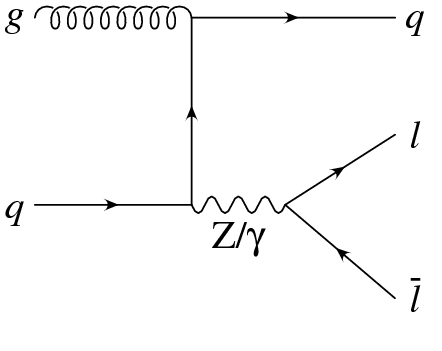
\includegraphics[width=.4\linewidth]{figures/xsection/ZJetsDiagram.png}
    }
    \subfigure[$W+Jets$]{
      % 
      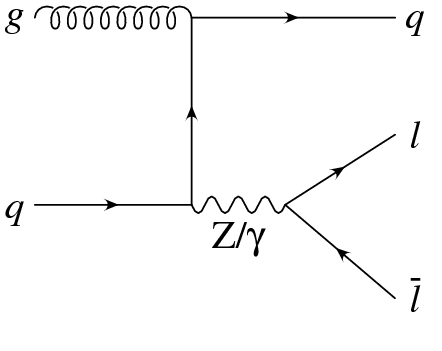
\includegraphics[width=.4\linewidth]{figures/xsection/ZJetsDiagram.png}
    } \\
    \subfigure[$QCD$]{
      %ZJetsDiagram.png : http://inspirehep.net/record/871058/files/qg_qZ.png
      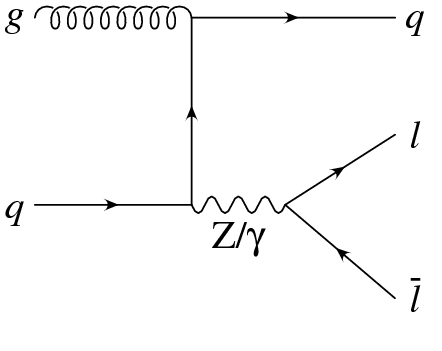
\includegraphics[width=.4\linewidth]{figures/xsection/ZJetsDiagram.png}
    }
    \subfigure[$Single Top$]{
      % 
      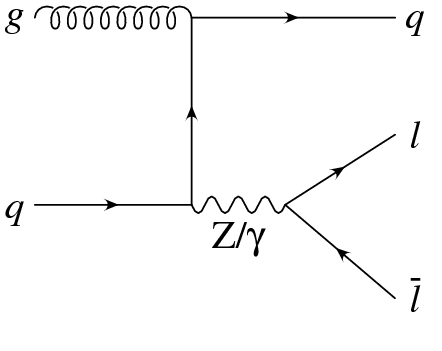
\includegraphics[width=.4\linewidth]{figures/xsection/ZJetsDiagram.png}
    } \\
  \end{center}
  \caption{Feynman diagrams for the most important backgrounds to $\ttbar$ events.  Shown are $Z+Jets$ events (top, left), $W+jets$ events (top, right), QCD events (bottom, left) and Single Top events (bottom, right).}
  \label{img:BackgroundsFeynmanDiagrams}
\end{figure}

To measure the cross-section, the background contributions due to each of the above processes in the lepton+jets channel were determined using a variety of techniques.


\subsection{Dilepton}


\subsection{Combination}





\section{Lepton+Jets}

The lepton$+$jets channel is the most statistically powerful decay of the $\ttbar$ system for measuring the pair-production cross-section.
The leptonic decay of one of the top results in an event topologiy that allows for strong background discrimination, while the hadronic decay of the other top maintains a high branching ratio for this channel.
The distinguishing features of the lepton$+$jets channel is the presence of a high-pt lepton from the leptonic decay of a W boson,v$\MET$ from a neutrino, two b-jets from the decay $t \rightarrow W+b$, and two additional jets from the hadronic decay of a W boson.
This topology of event was selected for by first requiring a single lepton trigger, which either required an electron or a muon (reconstructed by the trigger) with $E_{T} > 20 GeV$ or $p_{T} > 18 GeV$, respectively.
The exact trigger required varied throught the run periods of 2011 as higher instintaneous luminosities required stricter lepton definitions to maintain a steady bandwidth of recorded events as selected by the trigger.
Selected events are required to have a primary vertex that consists of 5 or more tracks.
Each event must have exactly 1 selected electron or muon, and that lepton must match a corresponding object that fired a single-lepton trigger (events with more than 1 lepton fall into the dilepton channel, to be described in detail later).
The energy requirements for these objects were chosen to minimize any effects resulting from the trigger's online reconstruction.
A cut on $\MET$ is imposed, requiring $\MET > 35 GeV$ for the electron channel and $\MET > 25 GeV$ for the muon channel (the difference in the cut results from different background contributions to each channel from QCD events, which tend to have low values of $\MET$).
Additional cuts are made on the to reduce the contamination from QCD, which use a variable known as the ``W boson transverse mass'':
\begin{equation}
  m_{T}(W) = \sqrt(2 p_{T}^{l} p_{T}^{\nu} (1 - cos( \phi^{l} - \phi^{\nu}))),
\end{equation} 
where the $\MET$ vector is used to determine the kinematic variables of the neutrino, $p_{T}^{\nu}$ and $\phi^{\nu}$.
Using this definition, the event selection requires $m_{T}(W) > 25 GeV$ in the electron channel or $\MET + m_{T}(W) > 60 GeV$ in the muon channel.



\subsubsection{Backgrounds}
A selection of events based on the above criteria will be contaminated with several sources of backgrounds, including

\begin{itemize}
\item QCD Multijet events where a lepton is faked via a background mechanism
\item $W+Jets$ events where the W decays leptonically (leading to $\MET$) which includes real or fake b-jets
\item $Z+Jets$ events where one of the two leptons isn't identified and which includes real or fake b-jets
\item Diboson Events (WW, WZ, or ZZ events), that include some combination of leptonic decays of vector bosons, additional jets, and real or faked b-jets
\item Single Top events
\end{itemize}

% Add figures

\begin{figure}
  \begin{center}
    \subfigure[$W+Jets$]{
      % 
      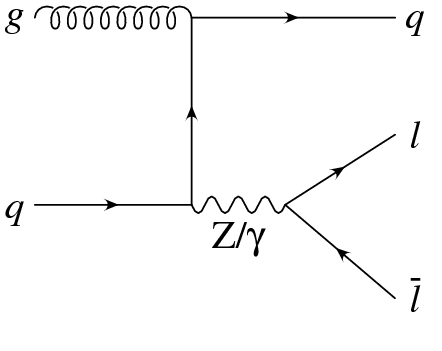
\includegraphics[width=.4\linewidth]{figures/xsection/ZJetsDiagram.png}
    }
    \subfigure[$QCD$]{
      %ZJetsDiagram.png : http://inspirehep.net/record/871058/files/qg_qZ.png
      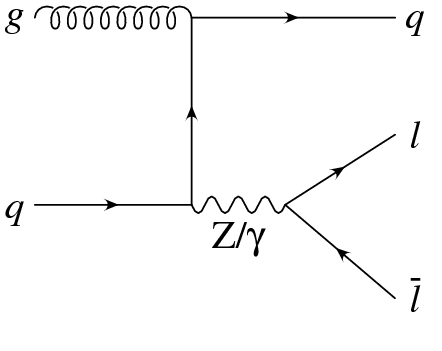
\includegraphics[width=.4\linewidth]{figures/xsection/ZJetsDiagram.png}
    } \\
    \subfigure[$Z+Jets$]{
      %ZJetsDiagram.png : http://inspirehep.net/record/871058/files/qg_qZ.png
      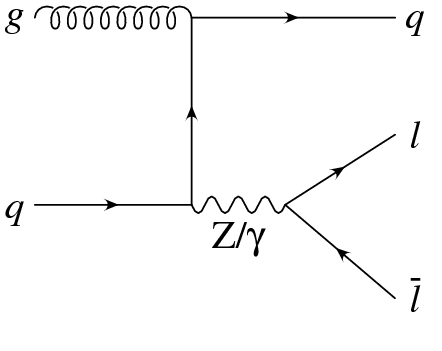
\includegraphics[width=.4\linewidth]{figures/xsection/ZJetsDiagram.png}
    }
    \subfigure[$Single Top$]{
      % 
      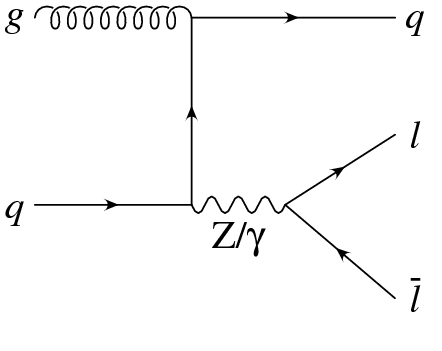
\includegraphics[width=.4\linewidth]{figures/xsection/ZJetsDiagram.png}
    } \\
  \end{center}
  \caption{Feynman diagrams for the most important backgrounds to $\ttbar$ events.  Shown are $Z+Jets$ events (top, left), $W+jets$ events (top, right), QCD events (bottom, left) and Single Top events (bottom, right).}
  \label{img:BackgroundsFeynmanDiagrams}
\end{figure}

To measure the cross-section, the background contributions due to each of the above processes in the lepton+jets channel were determined using a variety of techniques.
The dominant $W+Jets$ background as well as the $Z+Jets$, diboson, and single-top background are estimated using Monte-Carlo simulation.
While the kinematic distributions of each $W+Jets$ event were estimated from Monte-Carlo, the expected number of events was extracted using a data-driven technique.
The technique used to estimate the normalization of the $W+Jets$ background is based on one used in a top-quark charge-asymmetry analysis \cite{CHARGE_ASYMMETRY}.
It is based on the fact that $W^{+}$ bosons are produced at a higher rate than $W^{-}$ bosons due to the fact that the LHC collides protons (and not anti-protons).
The ratio of the production of $W^{+}$ to $W^{-}$, $r_{MC}$, can be estimated using Monte-Carlo.  Assuming that $W+Jets$ events are the dominant category of events that are asymmetric between positive and negative leptons, one can estimate the total number of $W+Jets$ events by taking the difference between the measured jumber of events with a positive lepton and the number with a negative lepton:

\begin{equation}
  N_{W^{+}} + N_{W^{-}} = \frac{r_{MC} + 1}{r_{MC} - 1}(D^{+} - D^{-}),
\end{equation}

where $D^{+}$ and $D^{-}$ are the number of selected single-lepton events with a positive or negative lepton, respectively.
The value of $r_{MC}$ is measured to be 1.56 $\pm$ 0.07 for the electron channel and 1.66 $\pm$ 0.06 for the muon channel.
Estimates of overall yields or kinematic variables for the $W+Jets$ background are then weighted to a total normalization given by this data-driven value.
The normalizations for the $Z+Jets$, diboson, and single-top backgrounds are taken directly from cross-sections evaluated using monte-carlo and scaled to the integrated luminosity recorded by the ATLAS detector.

Each of the backgrounds which are estimated using Monte-Carlo lead to real leptons in the final state.
In contrast, the QCD background enters the single-lepton channel when a final state jet is falsely identified as a lepton.
The process of a jet faking a lepton depends on the details of the jet's hadronic shower, in particular it's shape and depth in both the electromagnetic and hadronic calorimeters.
The hadronic shower evolution is of course modeled in detail by simulations used by ATLAS.
However, small differences in the nature of that simulation can lead to significant changes in the rate of jets faking leptons.
And because the number of QCD events created at ATLAS is extremely large, changes in the rate will have dramatic differences in the number of background events in the lepton+jets signal region.
For this reason, it is preferable to estimate the background contribution due to QCD without relying on the details of the Monte-Carlo description of hadronic shower evolution.

The lepton+jets analysis uses a technique to extract the rate and distribution of QCD events from data directly.
Known as the ``Matrix Method,'' this technique exploits the fact that the efficiencies of real and fake leptons differ as a function of cuts on the reconstructed lepton's isolation and shower shape.
The technique involves creating two subsets of lepton identifications, denoted as ``loose'' and ``tight'' (with ``tight'' corresponding to the nominal selection requirements).
The Matrix Method relies on knowing the effecienciy for both real and fake leptons which pass loose selection to also pass the tight selection.
It uses these efficiencies as a discriminating variable to separate real and fake leptons.
As the matrix method is used extensively throughout the analyses that coprise this thesis, it is described in detail in appendix ~\ref{app:matrixmethod}.
%% \begin{equation}
%%   \epsilon_{real} = \frac{N^{tight}_{real}}{N^{loose}_{real}} and \epsilon_{fake} = \frac{N^{tight}_{fake}}{N^{loose}_{fake}},
%% \end{equation}

%% where $N^{tight}$ and $N^{loose}$ represent the number of events with tight or loose (and not tight) lepton, respectively, in the region of phase space where the efficiency is being measured.
%% Given these values, one can write a set of equations relating the number of events with a measured loose or tight lepton to the number  

%% \begin{eqnarray}
%%   \bar{N^{tight}} = \epsilon_{real} N_{real} + \epsilon_{fake} N_{fake} \\
%%   \bar{N^{loose}} = (1-\epsilon_{real}) N_{real} + (1-\epsilon_{fake}) N_{fake}.
%%   \label{eq:MatrixMethod}
%% \end{eqnarray}

%% The above equations can be inverted to obtain $N_{fake}$ and $N_{real}$, quantities we're interested in estimating, as a function of  $N^{tight}$ and $N^{loose}$, quantities that can be measured.
%% By solving and isolating the variables $N^{tight}_{real}$ and $N^{tight}_{fake}$ (which represent the real and fake lepton contributions to the tight, or signal, region), and expressing the solution as a matrix, we obtain the following:

%% \begin{eqnarray}
%%   N^{tight}_{real} = \frac{N^{tight} - \epsilon_{fake}N^{loose}}{\epsilon_{fake} - \epsilon_{real}} \\
%%   N^{tight}_{fake} = \frac{\epsilon_{real}N^{loose} - N^{tight}}{\epsilon_{fake} - \epsilon_{real}}
%% \end{eqnarray}

%% \begin{equation}
%% \begin{pmatrix} N^{tight}_{real} \\ N^{tight}_{fake} \\ \end{pmatrix} 
%%   = 
%%   \begin{pmatrix} 
%%     \frac{\epsilon_{real}}{\epsilon_{real} - \epsilon_{fake}} & \frac{-\epsilon_{real}\epsilon_{fake}}{\epsilon_{real} - \epsilon_{fake}} \\ 
%%     \frac{-\epsilon_{fake}}{\epsilon_{real} - \epsilon_{fake}} & \frac{\epsilon_{real}\epsilon_{fake}}{\epsilon_{real} - \epsilon_{fake}} \\ 
%%   \end{pmatrix}  
%%   \begin{pmatrix} N^{tight} \\ N^{loose} \\ \end{pmatrix}
%%   \label{eq:MatrixMethodInverted}
%% \end{equation}

%% One should note that the solution is linear in the number of tight or loose events.
%% In particular, this means that we can associate any given event (be it loose or tight) with a weight for real or fake, and these weights are simply the (1,1) and (2,1) elements of the matrix in equation \ref{eq:MatrixMethodInverted}.
%% Therefore, in the case that the $\epsilon$ values are functions of arbitrary variables associated with an event, one can still estimate the number of fakes in the tight (signal) region as:

%% \begin{equation}
%%   N^{tight}_{fake} = \sum_{e \in tight} (\frac{-\epsilon_{fake}}{\epsilon_{real} - \epsilon_{fake}}) + \sum_{e \in loose} (\frac{\epsilon_{real}\epsilon_{fake}}{\epsilon_{real} - \epsilon_{fake}})
%%   \label{eq:MatrixMethodSum}
%% \end{equation}

%% Equation \ref{eq:MatrixMethodSum} is used to estimate the amount of QCD multijet events that enter the signal region (assuming that all fakes in the loose or tight regions come from QCD Multijet events).
%Equation \ref{eq:MatrixMethodSum} is used to estimate the amount of QCD multijet events that enter the signal region (assuming that all fakes in the loose or tight regions come from QCD Multijet events).
In that estimation, loose electrons are defined identically as tight electrons, except their isolation cut is relaxed, requiring that $E_{T} < 6 GeV$ in a cone defined by $\Delta R = 0.2$.
Similarly, loose muons are identical to tight muons, but the cuts on $E_{T}$ and $p_{T}$ isolation are removed entirely.
The efficiencies for loose leptons, as defined above, to also pass tight requirements for both real and fake muons are measured directly in data.
To measure the efficiencies of real leptons, a collection of events dominated by $Z->ee$ or $Z->\mu\mu$ is created by selecting dilepton events where the invariant mass of the leptons is close to the mass of the Z-boson.
In such a sample, the efficiency can be measured directly.
For fake leptons, a sample of QCD multijet events is collected by selecting events with a single (loose) lepton, a jet, and by requiring $5 GeV < \MET <  60 GeV$ for electron events or $m_{T}(W) < 20 GeV$ and $m_{T}(W) + \MET < 60 GeV$ for muon events.
For muons, the efficiencies were paramaterized as a function of the muon's $p_{T}$ and $\eta$.
Contributions from $Z+Jets$ and $W+Jets$ in the QCD control regions were subtracted using Monte-Carlo estimates.

% e + Jets
\begin{table}
  \begin{tabular}{lccccc}
    \hline
    $e + Jets$ & 1 Jet & 2 Jet & 3 Jet & 4 Jet & $>=$ 5 Jets \\ 
    \hline
    $\ttbar$ & $225 \pm 15$ & $1005 \pm 32$ & $1934 \pm 44$ & $1835 \pm 43$ & $1463 \pm 38$ \\
    $W+Jets$ & $161600 \pm 400$ & $43170 \pm 210$ & $10840 \pm 100$ & $2486 \pm 50$ & $1032 \pm 32$ \\
    $QCD Multijets$ & $11000 \pm 5000$ & $4800 \pm 2400$ & $1600 \pm 800$ & $510 \pm 250$ & $117 \pm 89$ \\
    Single Top & $571 \pm 24$ & $711 \pm 27$ & $391 \pm 20$ & $156 \pm 13$ & $65 \pm 8$ \\
    $ZJets$ & $3732 \pm 61$ & $2444 \pm 49$ & $996 \pm 32$ & $333 \pm 18$ & $146 \pm 12$ \\
    Diboson & $599 \pm 25$ & $538 \pm 23$ & $178 \pm 13$ & $45 \pm 7$ & $10 \pm 3$ \\
    \hline
    Total Predicted & $177000 \pm 5000$ & $52600 \pm 2400$ & $15900 \pm 800$ & $5360 \pm 260$ & $2892 \pm 100$ \\
    Total Observed & 179469 & 51820 & 15614 & 5398 & 2812 \\
    \hline
  \end{tabular}
  \caption{Predicted and observed event yields in bins of jet number for the $\ttbar$ signal and backgrounds in the $e+jets$ channel.  Yields are obtained using Monte Carlo or Data-Driven techniques, depending on the sample.}
\end{table}

% mu + Jets
\begin{table}
  \begin{tabular}{lccccc}
    \hline
    $e + Jets$ & 1 Jet & 2 Jet & 3 Jet & 4 Jet & $>=$ 5 Jets \\ 
    \hline
    $\ttbar$ & $319 \pm 18$ & $1342 \pm 37$ & $2734 \pm 52$ & $2714 \pm 52$ & $2030 \pm 45$ \\
    $W+Jets$ & $383200 \pm 600$ & $93440 \pm 310$ & $20140 \pm 140$ & $4644 \pm 68$ & $1082 \pm 33$ \\
    $QCD Multijets$ & $25000 \pm 12000$ & $11000 \pm 6000$ & $3200 \pm 1600$ & $900 \pm 400$ & $290 \pm 150$ \\
    Single Top & $996 \pm 32$ & $1148 \pm 34$ & $594 \pm 24$ & $210 \pm 15$ & $84 \pm 9$ \\
    $ZJets$ & $17270 \pm 130$ & $5492 \pm 74$ & $1510 \pm 39$ & $436 \pm 21$ & $149 \pm 12$ \\
    Diboson & $1093 \pm 33$ & $1009 \pm 32$ & $308 \pm 18$ & $69 \pm 8$ & $18 \pm 4$ \\
    \hline
    Total Predicted & $428000 \pm 12000$ & $113000 \pm 6000$ & $28400 \pm 1600$ & $8900 \pm 400$ & $3660 \pm 160$ \\
    Total Observed & 433931 & 111741 & 28643 & 8680 & 3814 \\
    \hline
  \end{tabular}
  \caption{Predicted and observed event yields in bins of jet number for the $\ttbar$ signal and backgrounds in the $\mu+jets$ channel.  Yields are obtained using Monte Carlo or Data-Driven techniques, depending on the sample.}
\end{table}


\begin{figure}
  \begin{center}
    \subfigure[$e+jets$] {
      % EJetsYieldPlot.eps: https://atlas.web.cern.ch/Atlas/GROUPS/PHYSICS/CONFNOTES/ATLAS-CONF-2011-121/fig_01a.eps
      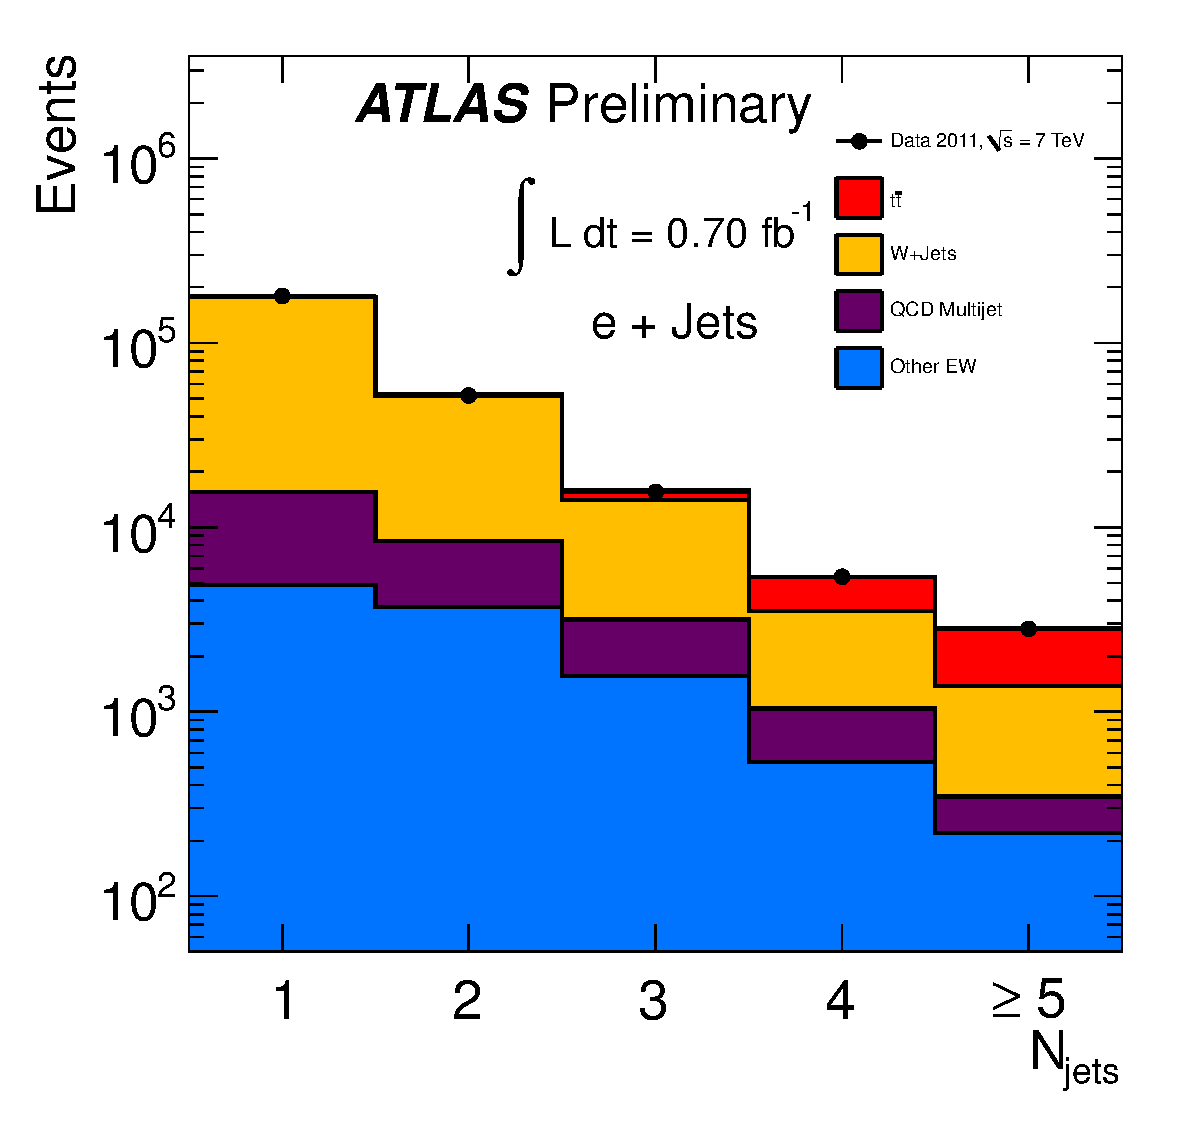
\includegraphics[width=.45\linewidth]{figures/xsection/EJetsYieldPlot}
    }
    \subfigure[$\mu+Jets$] {
      % MuJetsYieldPlots.eps: https://atlas.web.cern.ch/Atlas/GROUPS/PHYSICS/CONFNOTES/ATLAS-CONF-2011-121/fig_01b.eps
      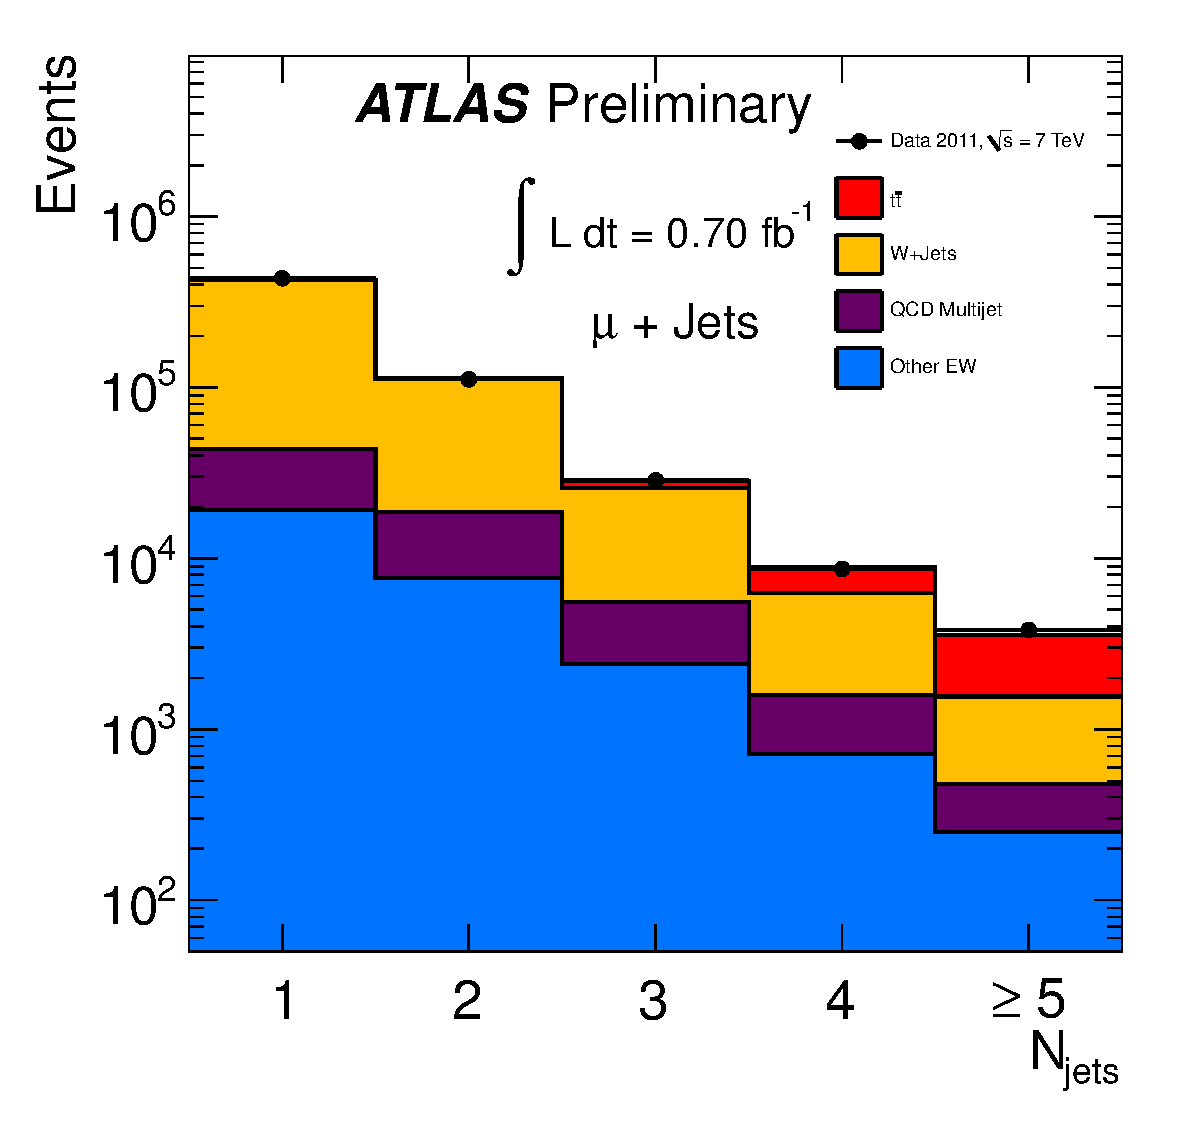
\includegraphics[width=.45\linewidth]{figures/xsection/MuJetsYieldPlot} %  figures/xsection/MuJetsYieldPlots}
    }
  \end{center}
  \caption{The yields of signal and backgrounds in bins of jet number.}
  \label{img:JetNumberYieldPlots}
\end{figure}


% https://atlas.web.cern.ch/Atlas/GROUPS/PHYSICS/CONFNOTES/ATLAS-CONF-2011-121/fig_01a.eps
% https://atlas.web.cern.ch/Atlas/GROUPS/PHYSICS/CONFNOTES/ATLAS-CONF-2011-121/fig_01b.eps


The measurement of the $\ttbar$ cross-section is obtained by fitting multiple multivariate distributions to measured data simultaneously.
These distributions are built out of four kinematic variables: the pseudorapidity of the selected lepton, the $p_{T}$ of the jet with the highest $p_{T}$, the event aplanrity and a variable denoted as $H_{T,3p}$.
The aplanarity, $A$, is defined as 1.5 times the smallest eivenvalue of the matrix

\begin{equation}
  M_{i,j} = \frac{ \sum_{k=1}^{N'_{objects}} p_{ik}p_{jk} }{ \sum_{k=1}^{N'_{objects}} p_{k}^2 }
  \label{eq:Aplanarity}
\end{equation}

and $H_{T, 3p}$, which is the total transverse momentum of all jets except for the first two normalized to the longitudinal momenta of all objects, is given by:

\begin{equation}
  H_{T, 3p} = \frac{ \sum_{i=3}^{N_{jets}} |p_{T, i}| }{ \sum_{j=1}^{N_{objects}} |p_{Z,j}|  }
\end{equation}


\begin{figure}
  \begin{center}
    \subfigure[leading jet $p_{T}$] {
      % DiscrimPtjet4Jets: https://atlas.web.cern.ch/Atlas/GROUPS/PHYSICS/CONFNOTES/ATLAS-CONF-2011-121/fig_04c.eps
      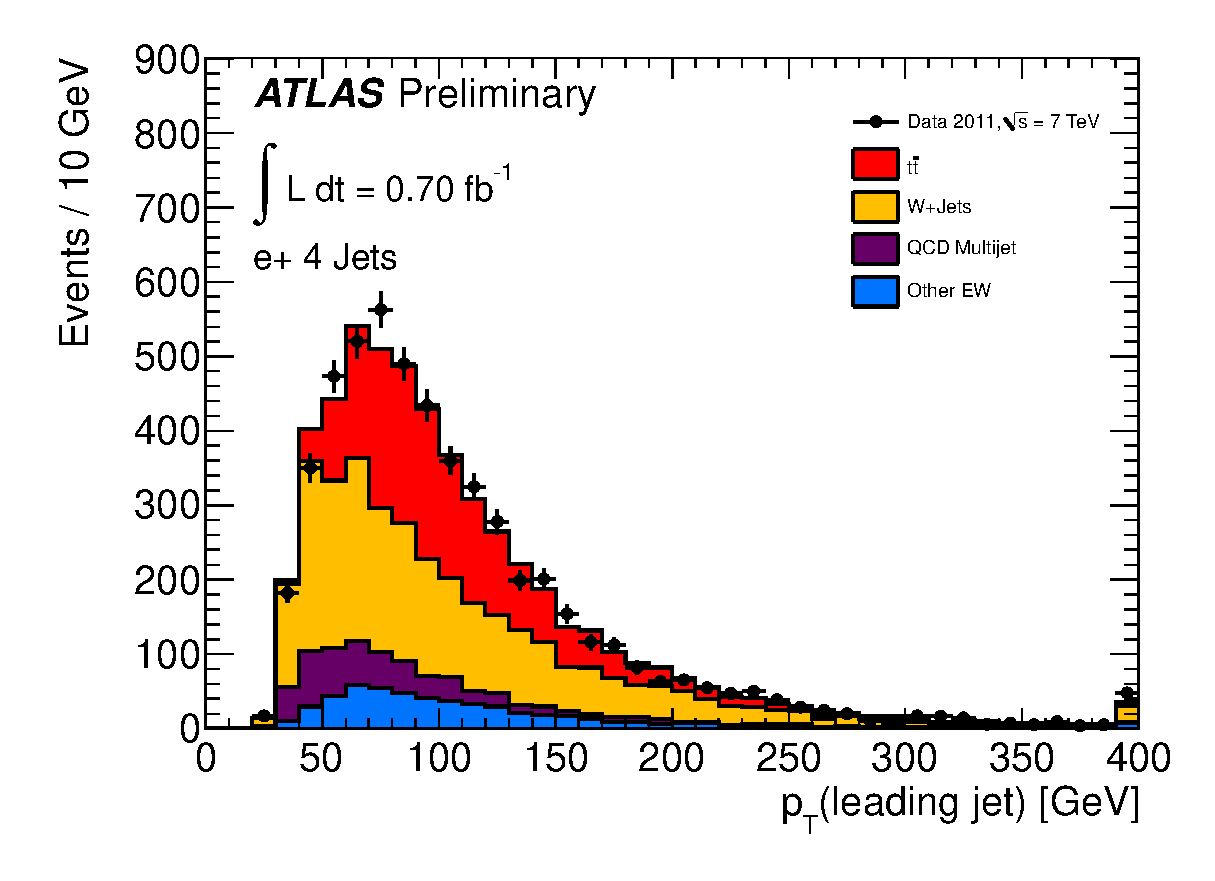
\includegraphics[width=.45\linewidth]{figures/xsection/DiscrimPtjet4Jets}
    }
    \subfigure[lepton ${\eta}$] {
      % DiscrimEtaMu4Jets
      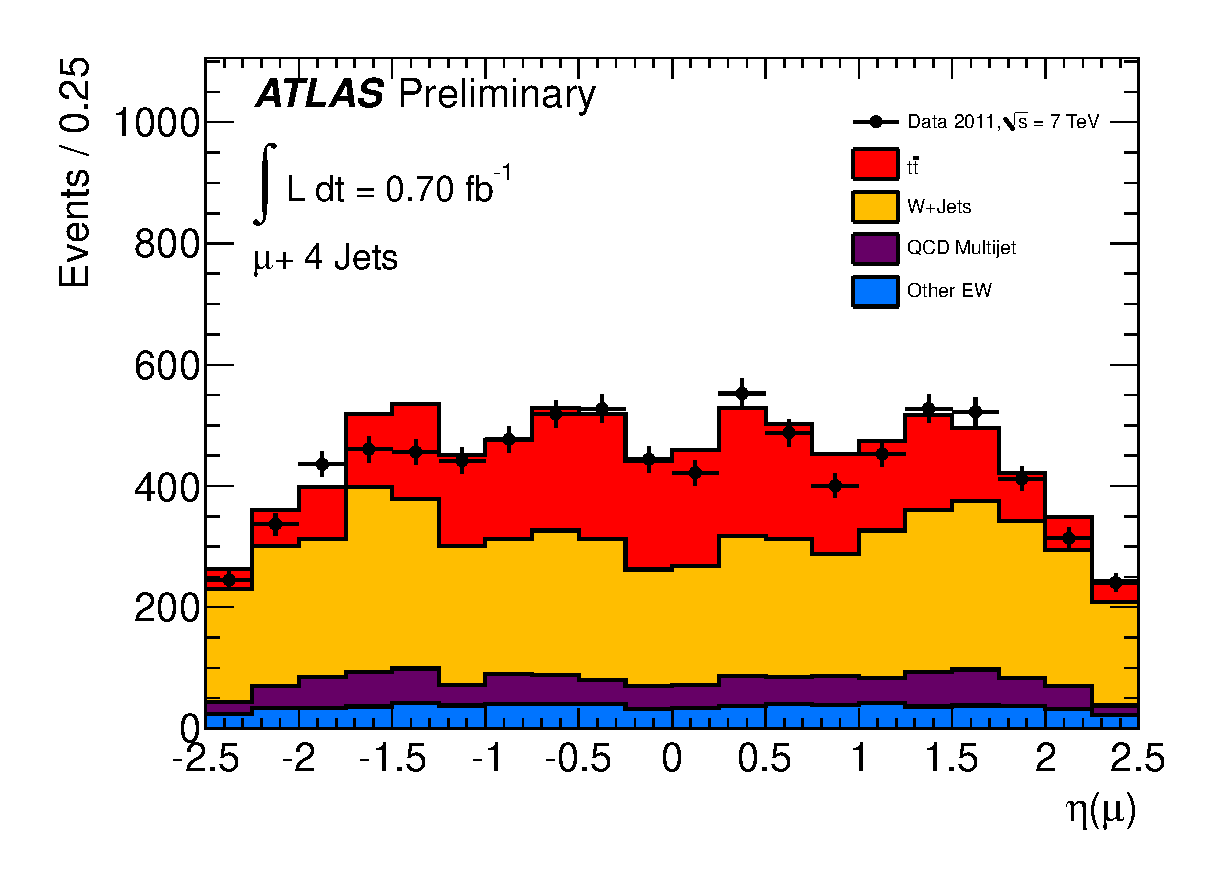
\includegraphics[width=.45\linewidth]{figures/xsection/DiscrimEtaMu4Jets}
    } 
    \subfigure[Aplanarity] {
      % 
      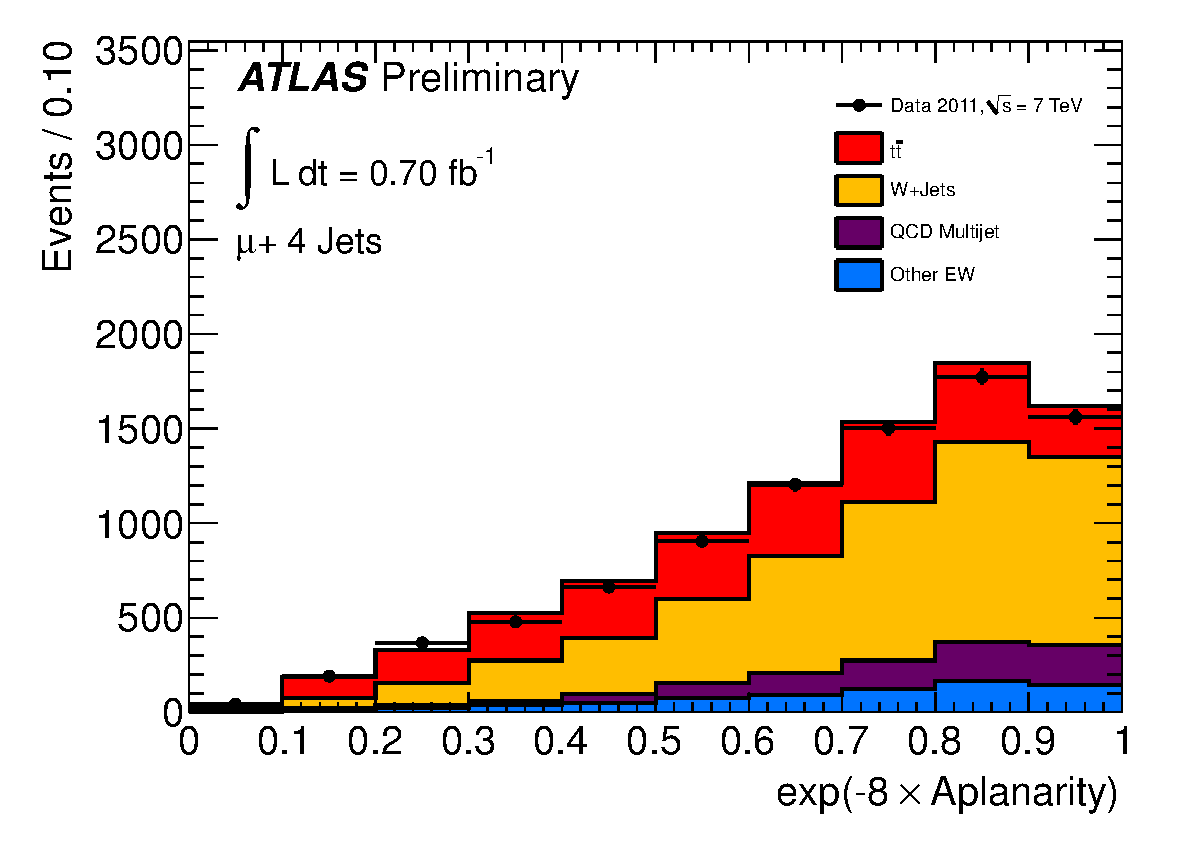
\includegraphics[width=.45\linewidth]{figures/xsection/DiscrimAplanarity4Jets}
    }
    \subfigure[$H_{T,3p}$] {
      % 
      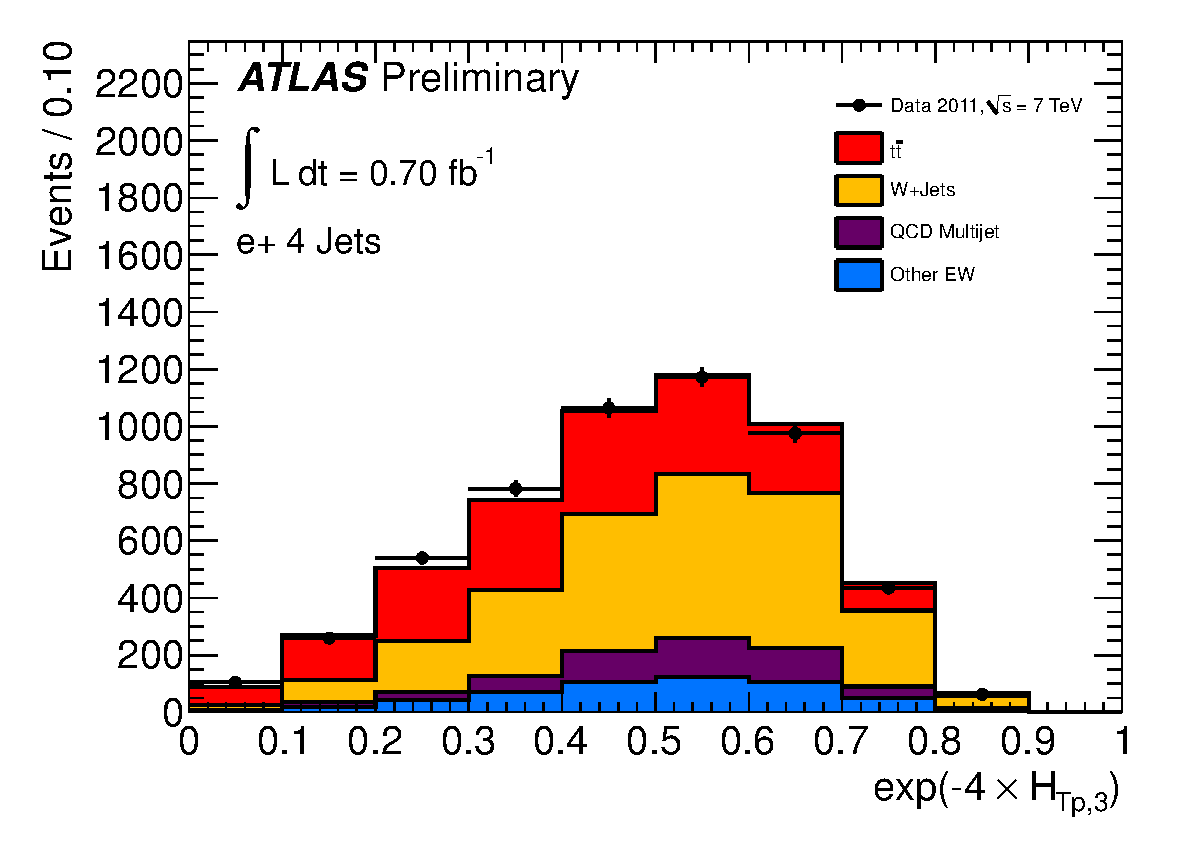
\includegraphics[width=.45\linewidth]{figures/xsection/DiscrimHT34Jets}
    } 
  \end{center}
  \caption{The discriminating variables used in the multivariate likelihood.}
  \label{img:DiscriminatingVariables}
\end{figure}


\begin{figure}
  \begin{center}

    \subfigure[] {
      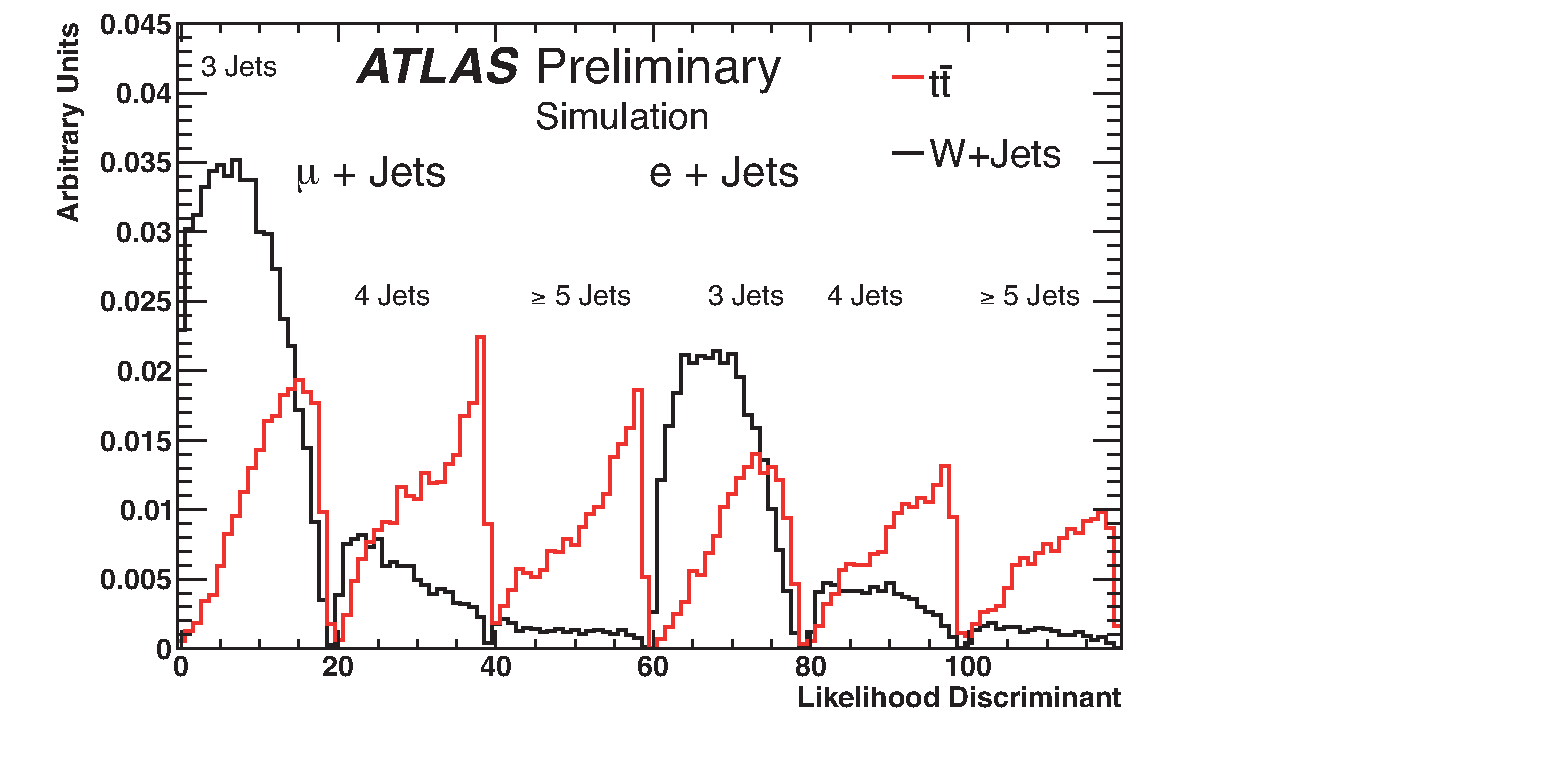
\includegraphics[width=.95\linewidth]{figures/xsection/LJetsDiscriminantLikelihood}
    }
    \subfigure[] {
      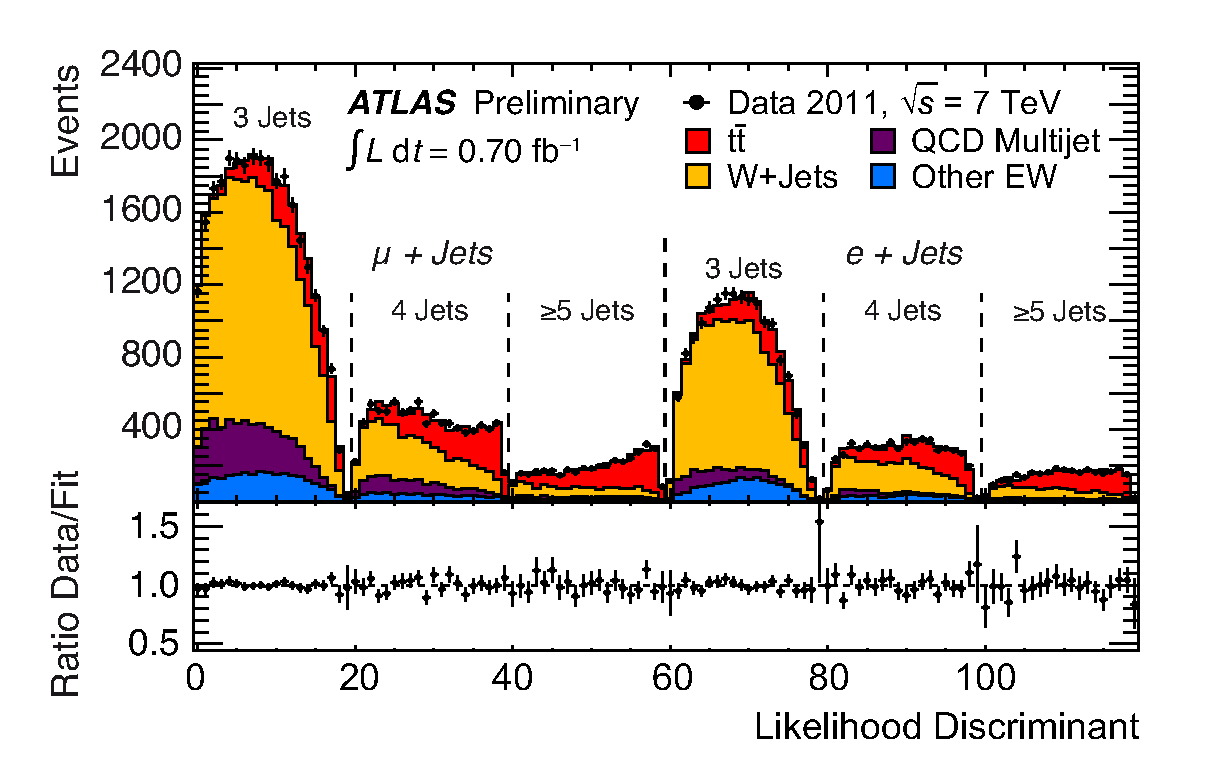
\includegraphics[width=.95\linewidth]{figures/xsection/LJetsFittedLikelihoodDiscriminant}
    }
  \end{center}
  \caption{The multivariate discriminant for $\ttbar$ signal and the dominant $W+Jets$ background.  Distributions are normalized to emphacize the difference in shape between signal and background.}
  \label{img:LJetsLikelihoodDiscriminant}
\end{figure}


\subsection{Systematic Uncertainties}

% The careful and consistent of the effect of systematic uncertainties and their proper paramaterization in a likelihood are crucial to making precise measurements.
The expected distribution of the discriminating variable in each channel and both signal and each background are sensitive to differences in theortical predictions and modeling of experimental effects.
Differences in the expected distributions will lead to differences in the measured cross-section.
Therefore, to incorporate theoretical and experimental uncertainties that will effect the measured cross-section, the expected distributions of the discriminating variable (including their normalizations as a function of integrated luminosity) are paramaterized by a number of terms that each represent on source of systematic uncertainty.
The likelihood function includes the effect of these parameters on the expected distributions as well as terms constraining these parameters, where the level of constraint comes from additional measurements that are made to gauge the size of these systematic uncertainties.
In the lepton+jets analysis, these constraints are modeled as gaussian terms with a mean of 0.0 and a variance of 1.0 (or rather, each paramater is scaled such that its constraint terms can be modeled in this way).

In the lepton+jets analysis, these uncertainties fall into several categories.  
Uncertainties on the cross-sections of backgrounds estimated using monte-carlo lead directly to uncertainties on the number of expected events in each bin of the discriminating variable for a fixed integrated luminosity.
These uncertainties on the cross-sections of the diboson, single-top and Z$+$Jet processes are determined by theoretical studies using Monte-Carlo simulation.
Uncertainties on the normalizations of the data-driven W$+$Jets and QCD backgrounds come from the propogation of statistical uncertainties through the data-driven techniques.
These data-driven normalization uncertainties are considered to be uncorrelated across in the 3 Jets, 4 Jets, and 5+ Jets channels (meaning, the effect is modeled by a separate parameter for each channel, and these parameters each have separate constraint terms and are allowed to move independently in a fit).

Uncertainties on the identification, reconstruction, and measurement of physical objects (jets, leptons, and $\MET$) effect the number of events that are selected, which channels those events may fall into, and the shape of discriminating variables within that channel.
These uncertainties include the energies of reconstructed objects as well as the rate at which they are triggered and identified.
Uncertainties on the measured energies of particles include uncertainties on both the energy scale and the energy resolution (roughly, these correspond to the mean and width of the distribution of measured energy, respectively).
The size of the uncertainties on object energy scale and energy resolution are paramaterized by a number of object variables, but most important are their position in the detector (in $\eta$ and $\phi$) and their nominal measured energy.
The effect of energy uncertainties are estimated by rescaling or randomly smearing the energy of objects in Monte-Carlo and obtaining new histograms of the discriminating variables for each background and sample.
Two such sets of template histograms are created for each source of systematic uncertainty corresponding to the effect of a +1 sigma and -1 sigma shift in these parameters (in addition to the nominal histograms, which in this language correspond to a 0 sigma shift in all systematic uncertainties).
The shapes of discriminating histograms for arbitrary shifts in uncertainty parameters are obtained by interpolating between these templates.
Furthermore, uncertainties in the Jet Energy Scale are broken down into subcomponents which consider separately uncertainties on the JES due to the calorimeter, uncertainties due to extrapolating from a low b-jet region to a high b-jet region, the dependence of calibration on pseudorapidity, the modeling of jets across generators, the effect of pile-up, and the effect of the underlying event.

Similarly, uncertainties on the rate at which leptons are identified and triggered are paramaterized by the object's location and energy.
The effect of these uncertainties on the expected distribution of signal and background events estimated from Monte-Carlo are estimatied by scaling the weight of individual events by a factor corresponding to the estimated difference between trigger, reconstruction, and identification rates between Monte-Carlo and data.
These scale factors are derived by studying known processes in data and comparing these processes to Monte Carlo (for leptons, these measurements are performed using Z boson events, where one can create a set of events with a high rate of real to fake leptons).

In addition, uncertainties on the modeling of initial and final state radiation (isr and fsr) in Monte-Carlo, the development of parton showers, and a term generally describing the difference between Monte-Carlo generators.
Finally, uncertainties due to finite Monte-Carlo statistics used to estimate the shapes of backgrounds are considered.

%  W+jets and QCD normalizations are fitted (unconstrained)
%


\subsubsection{Likelihood}

The expected value of the discriminating variable is estimated for every background sample, for every channel, and across all bins.
Using this information, a likelihood function for the measured data in the signal and control regions is created:

\begin{equation}
% L(⃗β, ⃗δ) = 􏰁 P(μk , nk ) × 􏰁 G(β j , ∆ j ) × 􏰁 G(δi , 1)
  L(\vec{\beta}, \vec{\delta}) = \prod Pois(n_{k},\mu_{k}(\vec{\beta},\vec{\delta})) \prod Gauss(\delta_j, \beta_j) \prod( 1, \delta_i),
\end{equation}

where $n_k$ are the values measured in data of each bin of the observable, $\mu_k$ is the expected value of each bin based on a combination of Monte Carlo and data-driven techniques, including the effects of systematic uncertainties.
The systematic uncertainties are paramaterized by two sets of parameters: $\vec{\beta}$, which represent the overall normalizations of backgrounds, and $\vec{\delta}$, which describe various experimental or theoretical uncertainties.

The measured value of the $\ttbar$ cross-section is taken to be the maximum likelihood estimator obtained by fitting the full likelihood, including all channels and systematic parameters, to the observed data distributions.
The uncertianty of this measurement is estimated by finding the interval bounded by the points where the negative log of the profile likelihood ratio crosses $\frac{1}{2}$.

In the context of the lepton$+$jets analysis, a number of the above uncertainties are not considered to be continuous, and therefore one cannot assign a single parameter to describe their effect.
These uncertainties come from differences in the monte-carlo generator used, the hadronization settings, the shapes of the QCD and EW backgrounds, and the effect of finite monte-carlo statistics.
Therefore, these uncertainties are not paramaterized in the lepton+jets likelihood.
Instead, they are evaluated outside of the likelihood fit by generating toy data and evaluating the difference in the uncertainty on the top quark cross-section due to their inclusion.
These uncertainties are later added in quadrature to the uncertainty obtained from the likelihood fit to obtain the total uncertainty on the measured cross-section.


\subsubsection{Results}

This likelihood function, which simultaneously describes all bins across channels for the discriminating variables, is fit to the observed data.
The fitted value of the $\ttbar$ cross section and its uncertainties due to statistical, systematic, and luminosity effects, is found to be $\sigma_{\ttbar} = 179.0 ^{+7.0}_{-6.9}(stat+sys) \pm 6.6 (lumi)$ pb.

Additional uncertainties that are not paramaterized in the Likelihood were added in quadrature to the fitted uncertainties.
These additional uncertainties consist of Generator Hadronization, QCD shape, W shape, and Monte Carlo statistics.

Including these effects, the total uncertainty on the measurement is given by:

$\sigma_{\ttbar} = 179.0 \pm 9.8 (stat + syst) \pm 6.6 (lumi) pb = 179.0 \pm 11.8$ pb.

%%  σtt ̄ =
%% 179.0+7.0 (stat + syst) ± 6.6 (lumi) pb .

%% The combined fit of the six analysis channels to the likelihood discriminant distribution in data in-
%% cluding all systematic uncertainties treated within the fit yields a tt ̄ production cross section of σtt ̄ =
%% 179.0+7.0 (stat + syst) ± 6.6 (lumi) pb . The result of the fit is shown in Fig. 7 and demonstrates an excel- −6.9
%% lent agreement between data and the background and tt ̄ signal model. After including uncertainties that are not part of the fit, σtt ̄ is measured to be
%% σtt ̄ = 179.0±3.9 (stat)±9.0 (syst)±6.6 (lumi) pb = 179.0±9.8 (stat + syst)±6.6 (lumi) pb = 179.0±11.8 pb.


\section{Dilepton}


\newcommand{\dr} {\ensuremath{\Delta R({\rm lepton},{\rm jet})}}
\newcommand{\pmasym}[2]{^{+#1}_{-#2}}
\newcommand{\sigmattbar}{\ensuremath{\sigma_{\ttbar}}}
\newcommand{\sigmaz}{\ensuremath{\sigma_{\Zboson}}}
\newcommand{\lumitot}{\mbox{0.70~fb$^{-1}$}}
\newcommand{\lumitotpm}{\mbox{0.70$\pm$0.03~fb$^{-1}$}}


%\newcommand{\sigmattbar}{\ensuremath{\sigma_{\ttbar}}}
%\newcommand{\sigmaz}{\ensuremath{\sigma_{\Zboson}}}
%\newcommand{\lumitot}{\mbox{0.70~fb$^{-1}$}}
%\newcommand{\lumitotpm}{\mbox{0.70$\pm$0.03~fb$^{-1}$}}
%cut & count numbers:
\newcommand{\xsectot}{171}
\newcommand{\xsecstat}{\pm 6}
\newcommand{\xsecsyst}{\pmasym{16}{14}}
\newcommand{\xseclumi}{\pm 8}

%cut & count w btagging numbers? or the simultaneous fit?
\newcommand{\xsecbtot}{177}
\newcommand{\xsecbstat}{\pm 6}
\newcommand{\xsecbsyst}{\pmasym {17}{14}}
\newcommand{\xsecblumi}{\pmasym {8}{7}}


\newcommand{\AKT}{anti-k$_{t}$}
\def\lum{{\ensuremath{\cal L}}}
\def \intlum {\int {\cal L} dt}
\def\MCatNLO{{\sc MC@NLO}}
\def\FigMerit{F_M}
\def\JetProb{{\sc JetProb}}
\def\SVZero{{\sc SV0}}
\def\Nn{N_n}  %  ntags in an event
\def\Zg{\Zboson/\gamma^{*}}
\def\GEANT{{\sc GEANT4}}



\subsection{Introduction}

While the branching ratio into the dilepton decay channel for top-quark pair production events
isn't as high as the lepton+jets channel, the presence of two high pt-leptons in the final state
makes this a powerful channel for precision measurements of top quark processes.

We here describe a measurement of the top-quark pair-production cross-section using the
dilepton final state, which is characterized by two high-pt, opposite-sign leptons,
significant missing energy due to the presence of neutrinos from the decay of W-bosons,
and two $b$-jets from the decay of the top quarks.


%% Top-quark production in dilepton final states has been studied using
%% proton-antiproton collisions at
%% $\sqrt{s}=1.96~\TeV$~\cite{Aaltonen:2010bs,Abazov:2009ae} and
%% Large Hadron Collider (LHC)
%% measurements of the production cross section in proton-proton
%% collisions at $\sqrt{s}=7~\TeV$ in the same final state have recently been
%% reported~\cite{Chatrchyan:2011nb,ATL-CONF-2011-034}.
%% A measurement is presented of the \ttbar\ production cross section
%% using the dilepton channel, characterized by two opposite-sign
%% leptons, unbalanced transverse momentum indicating the presence of
%% neutrinos from the $W$-boson decays, and two $b$-quark jets. This
%% result uses twenty times more data than the previous ATLAS measurement in the same final state,
%% reported in Ref.~\cite{ATL-CONF-2011-034}.

The high efficiency of lepton selection and the relatively small contribution of backgrounds
to the dilepton final state %combined with a requirement on a $b$-jet that further reduces background 
gives this channel a strong signal-to-background ratio.
The dilepton decay topology is divided into three sub-channels based on the flavor of the
final-state leptons.
The $ee$ channel contains two high-pt, isolated leptons identified using 
the inner detector and the electromagnetic calorimeter, the $\mu\mu$ channel contains two
high-pt, isolated muons which have been identified using the inner detector as well as the muon
spectrometer, and the $e \mu$ final state contains an electron and a muon.
These channels are mutually exclusive to facilitate their statistical combination.


%% The \ttbar~dilepton final states can be selected with a good
%% signal-to-background ratio using simple kinematic requirements.  With
%% the additional requirement of the
%% presence of a jet consistent with a $b$~quark
%% (`$b$-tag'), the signal-to-background ratio can be further improved.
%% Cross-section measurements with and without the $b$-tag requirement
%% are reported here.
%%  Leptons are either well-identified electron or
%% muon candidates that are selected using the full detector or, to
%% reduce losses from lepton identification inefficiencies, isolated
%% tracks.  The well-identified electrons or muons are called
%% `identified leptons', and the isolated tracks are referred to as
%% `track leptons'. The term `lepton' is used to refer to identified
%% leptons and track leptons collectively. Events with one identified
%% lepton and one track lepton are called `lepton+track' events.
%%   Each dilepton channel is
%% exclusive, i.e. has no overlap with the other channels. Channels
%% with tau leptons are not explicitly reconstructed, but reconstructed
%% leptons can arise from leptonic tau decays and a track lepton can
%% arise from hadronic tau decay modes as well.  The analysis with the
%% $b$-tag requirement uses only identified leptons.

The analysis uses collision data with a center-of-mass energy of
$\sqrt{s}$ = 7~\TeV\ from 2011, with an integrated luminosity of \lumitotpm~\cite{lumiPub, lumi}.
The main backgrounds considered in this analysis come from
$\Z$+jets events, events with a single top quark,
diboson events, and events with misidentified leptons originating from hadronic activity.
Background contributions from
$\Zg \rightarrow ee$+jets, $\Zg \rightarrow\mu\mu$+jets and events with
misidentified leptons are estimated using data-driven techniques, and all
other background estimations are obtained using Monte Carlo simulation.


%% The measured cross section takes into account the $\ttbar$\ signal
%% acceptance and the expected background contributions from
%% $\Zg$+jets, single top quarks, $WW$, $WZ$, and $ZZ$ events, and
%% events with misidentified leptons (primarily $W+$jets events).
%% Background contributions from
%% $\Zg\rightarrow ee$+jets, $\Zg\rightarrow\mu\mu$+jets and events with
%% misidentified leptons are evaluated
%% directly from the data. All other background contributions are
%% evaluated using Monte Carlo (MC) simulation samples.


\subsection{Monte Carlo Simulation}
\label{s:mc}


Monte Carlo simulation is used to estimate the production rate and kinematic distributions of the $\ttbar$ signal as well as several important background, 
and in addition it is used to evaluate the size of many important sources of systematic uncertianty.
All Monte Carlo samples used in this analysis were generated using \GEANT~\cite{geant4}\
to simulate the ATLAS detector.


%% Monte Carlo simulation samples are used to calculate the $\ttbar$\
%% acceptance and to evaluate the background contributions from single
%% top quarks, $WW$, $WZ$, and $ZZ$ events, and $\Zg
%% \rightarrow\tau\tau$+jets.
%% All MC samples are processed with the
%% \GEANT~\cite{geant4}\ simulation of the ATLAS detector~\cite{atlsim}\
%% and events are passed through the same analysis chain as the data.

Events containing top quarks, including the $\ttbar$ signal and the single-top background,
were generated using \MCatNLO\ generator~\cite{mcatnlo1,Frixione:2003ei,Frixione:2005vw}\
with the CTEQ6.6~\cite{cteq66}\ parton distribution function (PDF)
set and a top-quark mass of 172.5~\GeV.
However, the reference for the overall $\ttbar$ cross-section was calculated using
{\sc Hathor}\cite{Aliev:2010}, which employs an NNLO perturbative QCD calculation.


%% The generation of \ttbar{} and single top-quark events uses the
%% \MCatNLO\ generator~\cite{mcatnlo1,Frixione:2003ei,Frixione:2005vw}\
%% with the CTEQ6.6~\cite{cteq66}\ parton distribution function (PDF)
%% set and a top-quark mass of 172.5~\GeV. Expected $\ttbar$\ yields
%% are calculated with a cross section normalized to the prediction of
%% {\sc Hathor}\cite{Aliev:2010}, which employs an NNLO perturbative QCD calculation.
%% Single top-quark production with \MCatNLO\ includes the $s$, $t$ and
%% $Wt$ channels and the diagram-removal scheme~\cite{diagrem}\  is
%% used to reduce overlap with the $\ttbar$\ final state.

Drell-Yan events are simulated using the {\sc Alpgen} generator using
CTEQ6L1 \cite{cteq6l}\ to model the parton distribution function (pdf),
and the overall cross-section is scaled to the NNLO prediction, which
requires a scale factor (k-factor) of 1.25.
Diboson events are also modeled using the {\sc Alpgen}\ generator
and the overall cross-sections of the three categories of diboson events
were each individually scaled to match their predictions from NLO QCD,
which were calculated using the MCFM program~\cite{Campbell:1999ah}.

%% Drell-Yan events ($\Zg$+jets) are modeled with the {\sc Alpgen}
%% generator, using the MLM matching scheme~\cite{alpgen}\ and the
%% CTEQ6L1 \cite{cteq6l}\ PDF set. The $\Zg$+jets samples, including
%% both light and heavy flavor jets, are normalized to NNLO with a
%% $K$-factor of 1.25. %~\cite{CSCbook}.
%% In the $\Zg\rightarrow ee$ and $\mu\mu$ decay channels, the
%% background from $\Zg$+jets is evaluated using a data-driven
%% technique that normalizes the MC expectation to the data observation
%% near the $Z$ pole. Background contributions from the $W$+jets final
%% states come primarily from events where the $W$\ boson decays
%% leptonically and the second lepton candidate is a misidentified jet
%% or a heavy-flavor decay. Backgrounds from $W$+jets %and multijet
%% events are evaluated from the data.

All simulated event uses the {\sc Herwig} to model the parton shower ~\cite{herwig1,Corcella:2002jc}
as well as {\sc Jimmy} to simulate the effect of the underlying event model~\cite{jimmy}.
In addition, all events include additional background interactions, generated using Pythia,
to simulate the effect of in-time pile-up at the LHC.
Individual simulation events have been re-weighed so the overall distribution of
additional events due to pile-up matches the distribution measured in data.

%% All MC simulated events are hadronized using the {\sc Herwig}\ shower model~\cite{herwig1,Corcella:2002jc}\ supplemented by the
%% {\sc Jimmy}\ underlying event model~\cite{jimmy}.
%% Both hadronization programs are tuned to ATLAS data using the ATLAS MC10 tune~\cite{ATLAS:1303025}.
%% Diboson events are modeled using the {\sc Alpgen}\ generator normalized with
%% $K$-factors of 1.26 ($WW$), 1.28 ($WZ$) and 1.30 ($ZZ$) to match the total cross section from NLO QCD
%% predictions using calculations with the MCFM program~\cite{Campbell:1999ah}.

%% All Monte Carlo samples are generated taking into account that
%% multiple $pp$ interactions can occur in the same LHC bunch crossing
%% within a given event (`pile-up').  The MC events are re-weighted so
%% that the distribution of interactions per crossing in the MC matches
%% that observed in the data.  The average number of interactions per
%% crossing is 5.6 in this data set.


\subsection{Object selection}
\label{s:object}

The criteria for identifiying physical objects is consistent across the three dilepton sub-channels.
%Both electrons and muons are triggered using a single-lepton trigger

Electrons are identified as clusters in the electromagnetic calorimeter
that are matched to charged tracks in the inner-detector.
Electrons used in this analysis must meet the ``tight'' identification criteria,
which places strict requirements on the quality of the inner detector track and the
shape of the shower in the calorimeter.
Electrons are required to have $\pt>25\GeV$, are required to be within the range of the
optimal ATLAS inner detector, namely having $|\eta_{\text cl}|<2.47$ excluding the
transition region defined by $1.37<|\eta_{\text cl}|<1.52$.
Further, electrons are required to be isolated the electromagnetic calorimeter
by requiring that the transverse energy not associated with the electron within 
a radius defined by $\Delta R\equiv\sqrt{\Delta\eta^2 + \Delta\phi^2}$ must be less than $3.5\GeV$.

%% Lepton isolation requirements reduce backgrounds from misidentified
%% jets and suppress the selection of leptons from heavy-flavor decays.
%% For electron candidates, the transverse energy ($\ET$) deposited in
%% the calorimeter not associated to the electron is summed in a cone
%%  of radius $\Delta R = 0.2$, where
%% electron and is required to be less than $3.5\GeV$.


%% Leptons are required to be isolated and have high transverse
%% momentum, $\pt$, consistent with originating from $W$-boson
%% decay, with $\pt$ thresholds chosen to ensure events are triggered
%% with high efficiency.

%% Electron candidates are reconstructed from energy deposits
%% (clusters) in the EM calorimeter, which are then associated to
%% reconstructed tracks of charged particles in the inner detector.
%% Stringent quality requirements on the conditions of the EM
%% calorimeter at the time of data taking are applied to ensure a well measured reconstructed
%% energy. A `tight' selection~\cite{ElectronPerformance} using calorimeter,
%% tracking and combined variables, is employed to provide good
%% separation between the signal electrons and background.  Electron
%% candidates are additionally required to have $\pt>25\GeV$ and
%% $|\eta_{\text cl}|<2.47$, excluding electrons from the transition
%% region between the barrel and endcap calorimeters defined by
%% $1.37<|\eta_{\text cl}|<1.52$. The variable $\eta_{\text cl}$\ is
%% the pseudorapidity of the energy cluster associated with
%% the candidate.

Muons are required to contain a spectrometer track that matches a track in the inner detector.
They must have $\pt>20\GeV$ and $|\eta|<2.5$.
They are required to be energetically isolated both in the muon spectrometer and in the
inner detector.
The sum of the momenta of tracks having within $\Delta R = 0.3$\ and having $\pt>1$~GeV
must be no more than 4~GeV and the sum of transverse momentum within
a cone of $\Delta R = 0.3$\ must also be less than 4~GeV.
In addition, muons must be separated by at least $\Delta R > 0.4$\ from
selected jets wtih $\pt>20$~GeV, and potential muon pairs coming from
cosmic rays are eliminated by rejecting back-to-back muons with $|d_0|~>~0.5~$mm.

%% Muon candidate reconstruction is begun by searching for track
%% segments in
%%  layers of the muon chambers.
%% These segments are  combined starting from the
%% outermost layer, fitted to account for material effects, and matched
%% with tracks found in the inner detector.
%% The candidates are refitted using the complete track information from
%% both detector systems%~\cite{CSCbook}
%% , and required to satisfy $\pt>20\GeV$ and
%% $|\eta|<2.5$.

%For muon candidates, both the
%corresponding calorimeter isolation energy and the analogous track
%isolation, the sum of the track transverse momenta for tracks with
%$\pt>1$~GeV and in a cone $\Delta R = 0.3$\ centered on the lepton
%candidate, must be less than 4~GeV.

%% Additionally, muon candidates
%% must have a distance $\Delta R > 0.4$\ from any jet with
%% $\pt>20$~GeV, further suppressing muon candidates from heavy flavor
%% decays.
%% Muon candidates arising from cosmic rays are rejected by removing
%% candidate pairs that are back-to-back in the $r-\phi$ plane and
%% with transverse impact parameters relative to the beam axis
%% $|d_0|~>~0.5~$mm.

% Ignore Track Leptons

%% Track-lepton (TL) candidates are defined by an ID track with $\pt >
%% 25\GeV$ and a series of quality cuts optimized for high efficiency
%% and a low rate of misidentification. The track must have at least
%% six  SCT hits  and at least one hit in the innermost pixel layer. It
%% also must have $|d_0| < 0.2$~mm and the uncertainty on the momentum
%% measurement must be less than 20\%. The track has to be isolated
%% from other nearby tracks, following the track isolation defined above, in this case using
%%  tracks with $\pt>0.5\GeV$.  The summed momentum cut is set to 2~GeV.

Jets are reconstructed from energy clusters in the calorimeter using the {\it \AKT} algorithm~\cite{antikt}
with a radius parameter $R = 0.4$.
Jets are calibrated to the hadronic energy scale using $\eta$ and $\phi$ dependent corrections.
Because both jets and electrons are seeded by energy clusters in the calorimeter,
reconstructed jets within $\Delta R=0.2$\ of a selected electron are removed to
prevent double counting of physical objects.
Finally, jets are required to have $\pt>25$~GeV and $|\eta|<2.5$.

%% %of adjacent calorimeter cells.
%% These jets are then calibrated to
%% %by first
%% %correcting the jet energy using the scale established for
%% %electromagnetic objects and then performing a further correction to
%% the hadronic energy scale using $\pt$\ and $\eta$\ dependent
%% correction factors~\cite{jetcor}.
%% %Jets are removed if they are within $\Delta R=0.2$\ of a well-identified
%% %electron candidate. In lepton+track events, jets are removed if they are within $\Delta R=0.2$\ of a TL.
%% Jets are removed if they are within $\Delta R=0.2$\ of a well-identified
%% electron candidate or a TL.
%% The jets used in the analysis are required to have $\pt>25$~GeV
%% and $|\eta|<2.5$.


% We don't use b-tagging here
% My Writing:
%% Selected jet candidates can be further classified as originating from a
%% $b$-quark using an algorithm based on a likelihood ratio.
%% The likelihood discriminates bewteen $b$-jets and jets originating from
%% light quarks using a number of features, including the impact parameter
%% of the jet, the decay length significance associated with the secondary
%% vertex, the invariant mass of the tracks associated with the jet, 
%% and the ratio of the sum of energies of the tracks to the total
%% energy of the jet itself.
%% The classifier is designed to have an efficiency of $\approx 80\%$\
%% when applied to $b$-jets arising from $\ttbar$ events.


%% Jets are identified as $b$-quark candidates (`$b$-tagged') by an
%% algorithm that forms a likelihood ratio of $b$- and light-quark jet
%% hypotheses using the following discriminating variables: the signed
%% impact parameter significance of well measured tracks associated
%% with a given jet, the decay length significance associated with a
%% reconstructed secondary vertex, the invariant mass of all tracks
%% associated to the secondary vertex, the ratio of the sum of the
%% energies of the tracks associated with the secondary vertex to the
%% sum of the energies of all tracks in the jet assuming a pion
%% hypothesis, and the number of
%% two-track vertices that can be formed at the secondary
%% vertex~\cite{AdvBtag}. The cut on the combined likelihood ratio has
%% been chosen such that a $b$-tagging efficiency of $\approx 80\%$\
%% per $b$-jet in \ttbar~candidate events is achieved.
%and light quark as well as gluon jet rejection of order ten are achieved.

The missing transverse energy is formed by using the transverse 
momenta of jets, the calibrated transverse momenta of the cells of electron
candidates, muons, and calorimeter clusters not associated with a
reconstructed object.


%% The missing transverse momentum is formed from the negative vector
%% sum of transverse momenta of all jets with $\pt>20$~GeV and $|\eta|
%% < 4.5$~\cite{METPaper}. The contribution from cells associated with
%% electron candidates is replaced by the candidates' calibrated
%% transverse energy. The contribution from all muon candidates  and
%% calorimeter clusters (including those not belonging to a reconstructed
%% object) is also included.
%% The symbol $\MET$ is used to denote the magnitude of the
%% missing transverse momentum.


%
% HERE
%

\subsection{Event selection}
\label{s:event}

The dilepton analysis selects events based on the kinematic properties of the selected objects described above.
Events are triggered using inclusive single-lepton triggers that were present and unprescaled throughout
the 2011 data taking period.
To ensure a consistent understanding of trigger efficiency, the lepton feature that caused the trigger to fire
is required to be within $\Delta R < 0.15$ of a selected lepton.
Events are required to have a primary interaction vertex that has at least five tracks associated to it,
each of which must have a minimum of $\pt>400~\MeV$.
The entire event is rejected if a jet is considered likely to be the result of calorimeter noise or
if a jet is inconsistent with the timing of the bunch crossing~\cite{jetcor}.


%% The analysis requires collision data selected by an inclusive single
%% electron or muon trigger with offline-reconstructed
%% candidates satisfying $\pt>25\GeV$ for electrons, and $\pt>20\GeV$ for muons, to ensure a constant trigger efficiency.
%% To ensure that the event was triggered by the lepton candidates used
%% in the analysis,  one of the identified leptons and the triggered
%% lepton are required to match within $\Delta R < 0.15$.

%% Events are required to have a primary interaction vertex with at
%% least five tracks with $\pt>400~\MeV$.  The event is discarded if
%% any jet with $\pt>20$~GeV fails quality cuts designed to reject jets
%% arising from calorimeter noise or activity inconsistent with the
%% bunch-crossing time~\cite{jetcor}. If an electron candidate and a
%% muon candidate share a track, the event is also discarded.

The remaining kinmeatic selections on objects were chosen based on detailed studies
to minimize the expected uncertainty on the cross-section measurement before
considering the actual data measured.
The remaining selection requires:

%% The selection of events in the signal region consists of a series of kinematic requirements on
%% the reconstructed objects.
%% The requirements on $\MET$, the lepton-lepton invariant
%% mass ($m_{\ell\ell}$), and the scalar $\pt$ sum of all selected jets and leptons ($\HT$) are optimized
%% to minimize the expected total uncertainty on the cross-section measurement.
%% The resulting event selection, referred to as the `non-$b$-tag' selection, is listed below.

\begin{itemize}

\item Events must have exactly two oppositely-charged identified-lepton candidates ($ee$, $\mu\mu$,
  $e\mu$), satisfying the selection criteria of Section~4, {\em or} if only one identified-lepton candidate is found, the event is retained if a track-lepton candidate is present, with opposite charge to the identified lepton, forming a lepton+track event ($e$TL or $\mu$TL).

\item Events must have at least two jets with $\pT>25\GeV$ and $|\eta|<2.5$.%, no $b$-tagged jets are required.

\item Events in the $ee$, $\mu\mu$ $e$TL and $\mu$TL channels are required to have $m_{\ell\ell} > 15\GeV$ in order to
reject backgrounds from vector-meson decays. The requirement also helps to suppress backgrounds in these channels from $b$-quark production.

\item Events in the $ee$ and $\mu\mu$ channels must satisfy $\MET>60\GeV$ and $|m_{\ell\ell} - m_Z| > 10\GeV$,
to suppress backgrounds from $\Zg$+jets and multijets.

\item
Events in the $e\mu$ channel are required to satisfy $\HT>130\GeV$. No \MET\ or $m_{\ell\ell}$\ cuts are applied.
%In this case, remaining background from $\Zg$+jets production
%is suppressed by requiring $\HT>130~\GeV$.

\end{itemize}

%% A parallel selection with the additional requirement of at least one
%% $b$-tagged jet is made. Because of the enhanced background rejection
%% afforded by the $b$-tag requirement, the selection is further
%% optimized, resulting in an $\MET$\ requirement for $ee$ and $\mu\mu$
%% events that is relaxed to $\MET>40\GeV$, while the $\HT$\
%% requirement for $e\mu$ events remains the same as for the
%% non-$b$-tag selection, i.e. $\HT> 130\GeV$.  We refer to the
%% analysis that requires at least one $b$-tagged jet as the `$b$-tag
%% analysis', and the events selected therein as the `$b$-tagged
%% sample'.  The subset of the $b$-tagged sample with $40\GeV<
%% \MET<60\GeV$ is referred to as the `exclusive $b$-tagged sample' and
%% has no overlap with the non-$b$-tag sample.

Based on studies of Monte-Carlo simulation, the acceptance of this selection
on the $\ttbar$ signal is 0.96\% when averaged over all three channels.

%% The acceptance times the branching fraction of $\ttbar$ to
%% dileptons, for the selection described above, is 0.96\% for the $ee
%% + \mu\mu +e\mu$ channels without $b$-tagging, 0.11\% for the
%% exclusive $b$-tagged sample, and 0.19\% for $e$TL + $\mu$TL
%% channels.


\subsection{Background evaluation}
\label{s:backgrounds}

Although the event selection attempts to reject $\Zg$+jets events by requiring a minimum dilepton invariant mass of $15 GeV$ and exlcuding a
mass window within 10 GeV of the around the $Z$-boson, there remains a non-neglegive contribution to the signal region from this background.
Moreover, because these events have little ``real'' missing energy (which typically referrs to missing energy arising from neutrinos),
and the event selection requires a large amount of missing energy, $\Zg$+jets must have significant missing energy arising
from mismeasurements, which is channelging to model accurately using Monte-Carlo simulation.
For this reason, the size of this background is measured directly in-data using a control region, and the  contribution to the signal regions
is evaluated by extrapolating from that control region using a factor determined using Monte-Carlo~\cite{ATL-CONF-2011-034}..
This control region is identical to the signal region with the exception that it inverts the cut on the invariant mass of the reconstructed
lepton, requiring instead that they be within 10 GeV of the $Z$-boson mass.
In addition, the missing energy cut is relaxed to only require $\met>30~\GeV$.
The presence of signal and other backgrounds in this control region is corrected for using
Monte-Carlo simulation



%% The $\ttbar$ event selection rejects $\Zg$+jets
%% events with $ee$ and $\mu\mu$ invariant mass below $15 \GeV$, or within $10 \GeV$ of the $Z$-boson mass. However, $\Zg$+jets events with $ee$ or $\mu\mu$  invariant mass outside of these regions can enter the signal sample when there is large $\met$, typically from mismeasurement.
%% These events are difficult to properly model in simulations
%% due to uncertainties on the non-Gaussian tails of the $\met$\ distribution,
%% on the cross section for $Z$~boson production with multiple jets, and on the
%% lepton energy resolution.

%% To evaluate the $\Zg$+jets background in dielectron and dimuon events
%% ($Z \to \tau\tau$ is considered below), the MC prediction for the number of events in the signal region is normalized to the data using the number of
%% $\Zg$+jets events measured in a control region~\cite{ATL-CONF-2011-034}.
%% %orthogonal to the \ttbar\ dilepton signal region.
%% The control region is formed by
%% events with the same jet requirements as the signal region, but with
%%  $m_{\ell \ell}$ within 10 GeV of the $Z$-boson mass, and a $\MET$ cut of
%% $\met>45~\GeV$ for the lepton+track candidates and $\met>30~\GeV$
%% for the others. Contamination in the control region from other
%% physics processes (signal and other background processes considered
%% for the analysis) is subtracted according to MC predictions.
%% The ratio of data events to MC expectation in the control region
%% provides a scale factor that is used to correct the MC prediction
%% for $\Zg$+jets events in the signal region.

A number of sources of background enter the signal region due to a false postive reconstruction
of a lepton, which is referred to as a fake lepton.
The background due to fake leptons comes mostly from $W$+jets, \ttbar\, lepton+jets,
and single top-quark production.
The contribution to the signal region from these events is collectively evaluated
using the Matrix-Method (described in detail elsewhere) which uses loose and tight
leptons selections to disentangle the contribution to the signal region from 
real leptons from fake leptons.
The Matrix-Method requires knowing the reconstruction and identification efficiencies of both
real and fake leptons for both the loose and tight selections.
The efficiencies for real leptons to be identified as tight given that they are identified as loose
were measured using $\Zee$ and $\Zmm$ candidate events, and the efficiencies for fake leptons
(known as the fake rate) was measured using using $W$+jets events
The contribution of real leptons in the control region for measuring the fake rate was 
subtracted using estimates obtained from Monte Carlo.


%% Other backgrounds mainly come from $W$+jets, \ttbar\, lepton+jets,
%% and single top-quark production with fake leptons. The term `fake
%% lepton' is used to refer to both misidentified and non-prompt lepton
%% candidates, the latter category arising from hadron decays in
%% flight. The yield of events with fake identified leptons is
%% evaluated from the data using a matrix method~\cite{top2010}. In
%% addition to the standard lepton selection requirements, a selection
%% with a looser isolation requirement is defined.  Dilepton events are
%% selected using the loose isolation requirement and events are
%% categorized according to whether each lepton passes the standard
%% selection or the loose selection but not the standard selection.
%% There are four such categories for the two leptons: loose-loose,
%% loose-standard, standard-loose, and standard-standard.  Each of the
%% four categories is related to the number of events with two `real'
%% (prompt) leptons, two fake leptons, or one of each, through a set of
%% linear equations with coefficients given by the products of
%% probabilities for real or fake lepton satisfying the loose selection
%% to also satisfy the standard selection.  These linear expressions
%% form a matrix that is inverted in order to extract the real and fake
%% lepton content of the observed dilepton event sample.
%% The probability for real leptons is measured as a function of jet
%% multiplicity using data samples of
%% $\Zee$ and $\Zmm$ events.
%% The corresponding probability for
%% fake leptons is measured in a data sample dominated by dijet production,
%% with events containing one lepton candidate passing the looser isolation cuts and having $\met <20 \GeV$.
%% Contributions from real leptons due to $W$+jets final states are
%% subtracted using simulated events.

%% For lepton+track events the largest background is from events with
%% fake leptons, dominated by fake track leptons. The
%% probability of a jet being reconstructed as a track lepton is
%% determined from a $\gamma$+jets data sample selected with photon
%% triggers. The fake probability is applied to a second sample
%% enriched in $W$+jets events with exactly one identified lepton and
%% no track leptons, but using the same kinematic cuts as for the
%% signal sample. In this second sample the fake probabilities are
%% summed for each jet in each event and the fake track-lepton
%% contribution is calculated as a function of the number of jets.

The contributions of events with two real leptons and missing energy
distributions that are well-modeled using simulation, including
single top quarks, $Z \to \tau\tau$, $WW$, $ZZ$ and $WZ$, are evaluated
using Monte Carlo simulation.
The expected background rate in all three channels is given in table Table~\ref{t:signal}


%% The contributions from other electroweak background processes with
%% two real leptons,  such as single top quarks, $Z \to \tau\tau$,
%% $WW$, $ZZ$ and $WZ$ production are determined from Monte Carlo
%% simulations.   The expected numbers of background events are given
%% in Table~\ref{t:signal}.  The absence of $\Zg$+jets background in
%% the $e\mu$ channel, coupled with the larger branching fraction for
%% the $e\mu$ signal, allows relatively loose selection criteria to be
%% used in this channel. %The $b$-tagged $e\mu$ events require the same

%% The background contributions for the $b$-tag analysis are determined
%% using the same techniques described above, with the additional
%% requirement of a $b$-tagged jet.

%
% Consider including the below
%

%% The modeled acceptances, efficiencies and data-driven background
%% evaluation methods are validated by comparing predictions from Monte
%% Carlo simulations with data in control regions with kinematics
%% similar to the signal region but dominated by backgrounds. In
%% particular, the \met, $m_{\ell\ell}$ and jet multiplicity
%% distributions are studied in a sample of $Z$-boson candidates,
%% defined by requiring $|m_{\ell\ell} - m_Z| < 10 \GeV$ and $\met
%% <$~60 GeV. The predictions from MC simulations in the control
%% regions are in reasonable agreement with data, although small
%% discrepancies exist in regions that do not affect the $\ttbar$
%% cross-section measurement.


\newcommand{\DYZeeNJetsTwoJet}{$4.0^{+2.5}_{-1.2}$}
\newcommand{\DYZmmNJetsTwoJet}{$14.4^{+5.4}_{-4.2}$}
\newcommand{\ZtteeNJetsTwoJet}{4.9 $\pm$ 2.6}
\newcommand{\ZttmmNJetsTwoJet}{11.0 $\pm$ 5.0}
\newcommand{\ZttemNJetsTwoJet}{43 $\pm$ 16}
\newcommand{\FakeWeeNJetsTwoJet}{4.0 $\pm$ 5.0}
\newcommand{\FakeWmmNJetsTwoJet}{6.3 $\pm$ 4.1}
\newcommand{\FakeWemNJetsTwoJet}{44 $\pm$ 24}
\newcommand{\singletopeeNJetsTwoJet}{6.4$^{+1.2}_{-1.1}$}
\newcommand{\singletopmmNJetsTwoJet}{16.0$^{+1.9}_{-2.2}$}
\newcommand{\singletopemNJetsTwoJet}{41.1 $\pm$ 5.5}
\newcommand{\dibosoneeNJetsTwoJet}{5.9 $\pm$ 1.1}
\newcommand{\dibosonmmNJetsTwoJet}{8.7$^{+1.2}_{-1.5}$}
\newcommand{\dibosonemNJetsTwoJet}{32.9 $\pm$ 4.9}

\newcommand{\TotalNonttbaree}{25.2 $\pm$ 6.4}
\newcommand{\TotalNonttbarmm}{56.5 $\pm$ 9.4}
\newcommand{\TotalNonttbarem}{161 $\pm$ 34}

\newcommand{\ttbareeNJetsTwoJet}{124 $\pm$ 17}
\newcommand{\ttbarmmNJetsTwoJet}{$241^{+15}_{-18}$}
\newcommand{\ttbaremNJetsTwoJet}{746 $\pm$ 42}

\newcommand{\TotalExpectedee}{149 $\pm$ 18}
\newcommand{\TotalExpectedmm}{$298^{+17}_{-20}$}
\newcommand{\TotalExpectedem}{907 $\pm$ 54}

\newcommand{\DataeeNJetsTwoJet}{165}
\newcommand{\DatammNJetsTwoJet}{301}
\newcommand{\DataemNJetsTwoJet}{963}

%Lepton+track
\newcommand{\DYZeTLNJetsTwoJet}{$24.3^{+10.7}_{-9.4}$}
\newcommand{\DYZmTLNJetsTwoJet}{$22.0^{+5.3}_{-5.8}$}
\newcommand{\ZtteTLNJetsTwoJet}{$17.0^{+8.4}_{-7.6}$}
\newcommand{\ZttmTLNJetsTwoJet}{25 $\pm$ 11}
\newcommand{\FakeWeTLNJetsTwoJet}{74 $\pm$ 15}
\newcommand{\FakeWmTLNJetsTwoJet}{85 $\pm$ 17}
\newcommand{\singletopeTLNJetsTwoJet}{$5.7^{+1.0}_{-0.9}$}
\newcommand{\singletopmTLNJetsTwoJet}{$6.3^{+0.8}_{-1.1}$}
\newcommand{\dibosoneTLNJetsTwoJet}{$5.9^{+0.9}_{-0.8}$}
\newcommand{\dibosonmTLNJetsTwoJet}{$4.8^{+0.6}_{-0.7}$}

\newcommand{\TotalNonttbareTL}{$126^{+20}_{-19}$}
\newcommand{\TotalNonttbarmTL}{142 $\pm$ 21}

\newcommand{\ttbareTLNJetsTwoJet}{$112~^{+16}_{-18}$}
\newcommand{\ttbarmTLNJetsTwoJet}{$110~^{+17}_{-16}$}

\newcommand{\TotalExpectedeTL}{239 $\pm$ 26}
\newcommand{\TotalExpectedmTL}{253 $\pm$ 27}

\newcommand{\DataeTLNJetsTwoJet}{236}
\newcommand{\DatamTLNJetsTwoJet}{255}

%b-tag
\newcommand{\DYZeeNJetsTwoJetb}{$9.8^{+1.7}_{-1.3}$}
\newcommand{\DYZmmNJetsTwoJetb}{$20.3^{+1.8}_{-2.8}$}
\newcommand{\ZtteeNJetsTwoJetb}{$1.8^{+1.1}_{-1.2}$}
\newcommand{\ZttmmNJetsTwoJetb}{7.6$^{+3.3}_{-3.6}$}
\newcommand{\ZttemNJetsTwoJetb}{9.5$^{+4.2}_{-3.9}$}
\newcommand{\FakeWeeNJetsTwoJetb}{7.5 $\pm$ 6.5}
\newcommand{\FakeWmmNJetsTwoJetb}{4.9 $\pm$ 3.1}
\newcommand{\FakeWemNJetsTwoJetb}{20 $\pm$ 13}
\newcommand{\singletopeeNJetsTwoJetb}{7.3$^{+1.3}_{-1.1}$}
\newcommand{\singletopmmNJetsTwoJetb}{16.2$^{+2.2}_{-2.3}$}
\newcommand{\singletopemNJetsTwoJetb}{33.5$^{+4.8}_{-4.7}$}
\newcommand{\dibosoneeNJetsTwoJetb}{2.2 $\pm$ 0.7}
\newcommand{\dibosonmmNJetsTwoJetb}{2.6$^{+0.9}_{-0.6}$}
\newcommand{\dibosonemNJetsTwoJetb}{8.8$^{+1.7}_{-1.6}$}

\newcommand{\TotalNonttbareeb}{28.6 $\pm$ 6.9}
\newcommand{\TotalNonttbarmmb}{51.6$^{+5.6}_{-5.9}$}
\newcommand{\TotalNonttbaremb}{71.6 $\pm$ 14.1}

\newcommand{\ttbareeNJetsTwoJetb}{159$^{+17}_{-21}$}
\newcommand{\ttbarmmNJetsTwoJetb}{$304^{+26}_{-35}$}
\newcommand{\ttbaremNJetsTwoJetb}{675$^{+57}_{-75}$}

\newcommand{\TotalExpectedeeb}{188$^{+18}_{-22}$}
\newcommand{\TotalExpectedmmb}{$356^{+27}_{-35}$}
\newcommand{\TotalExpectedemb}{746$^{+59}_{-76}$}

\newcommand{\DataeeNJetsTwoJetb}{201}
\newcommand{\DatammNJetsTwoJetb}{365}
\newcommand{\DataemNJetsTwoJetb}{834}

\begin{table*}[htb]
\begin{footnotesize}
%\begin{adjustwidth}{-6em}{-6em}
\centering
\begin{tabular}{|l|c|c|c|} \hline
                          & $ee$                    & $\mu\mu$                & $e\mu$                  \\ [0.2ex] \hline
                          &                         &                         &                         \\ [-1.9ex]
$\Zg$+~jets               & \DYZeeNJetsTwoJet       & \DYZmmNJetsTwoJet       & -                       \\ [0.3ex]
$\Zg \to \tau\tau$+jets   & \ZtteeNJetsTwoJet       & \ZttmmNJetsTwoJet       & \ZttemNJetsTwoJet       \\ [0.3ex]
Fake leptons              & \FakeWeeNJetsTwoJet     & \FakeWmmNJetsTwoJet     & \FakeWemNJetsTwoJet     \\ [0.3ex]
Single top quark          & \singletopeeNJetsTwoJet & \singletopmmNJetsTwoJet & \singletopemNJetsTwoJet \\ [0.3ex]
Diboson                   & \dibosoneeNJetsTwoJet   & \dibosonmmNJetsTwoJet   & \dibosonemNJetsTwoJet   \\ [0.3ex] \hline
                          &                         &                         &                         \\ [-1.9ex]
Total background          & \TotalNonttbaree        & \TotalNonttbarmm        & \TotalNonttbarem        \\ [0.3ex]
Predicted \ttbar\         & \ttbareeNJetsTwoJet     & \ttbarmmNJetsTwoJet     & \ttbaremNJetsTwoJet     \\ [0.3ex] \hline
                          &                         &                         &                         \\ [-1.9ex]
Total                     & \TotalExpectedee        & \TotalExpectedmm        & \TotalExpectedem        \\ [0.3ex] \hline \hline
                          &                         &                         &                         \\ [-1.9ex]
Observed                  & \DataeeNJetsTwoJet      & \DatammNJetsTwoJet      & \DataemNJetsTwoJet      \\ \hline
\end{tabular}
%\end{adjustwidth}
\end{footnotesize}
\caption {Breakdown of the expected {\ttbar} signal and background
events in the signal region compared to the observed event yields,
for each of the dilepton channels. All systematic uncertainties are
included, and correlations between different background sources are
taken into account, when calculating the total background
uncertainty. The largest contribution to the line labeled 'Fake
leptons' comes from $W+$jets events.} \label{t:signal}
\end{table*}

%
% THEIRS:
%

%% \begin{table*}[htb]
%% \begin{footnotesize}
%% \begin{adjustwidth}{-6em}{-6em}
%% \centering
%% \begin{tabular}{|l|c|c|c|c|c||c|c|c|} \hline
%%                           & $ee$                    & $\mu\mu$                & $e\mu$                  & $e$TL                & $\mu$TL      & $b$-tag $ee$         & $b$-tag $\mu\mu$      & $b$-tag $e\mu$          \\ [0.2ex] \hline
%%                           &                         &                         &                         &                      &              &                      &                       &                         \\ [-1.9ex]
%%                           $\Zg$+~jets              & \DYZeeNJetsTwoJet       & \DYZmmNJetsTwoJet       & -                       & \DYZeTLNJetsTwoJet  & \DYZmTLNJetsTwoJet         & \DYZeeNJetsTwoJetb     & \DYZmmNJetsTwoJetb    & $-$                             \\ [0.3ex]
%% $\Zg \to \tau\tau$+jets  & \ZtteeNJetsTwoJet       & \ZttmmNJetsTwoJet       & \ZttemNJetsTwoJet       & \ZtteTLNJetsTwoJet  & \ZttmTLNJetsTwoJet                & \ZtteeNJetsTwoJetb            & \ZttmmNJetsTwoJetb     &  \ZttemNJetsTwoJetb           \\ [0.3ex]
%%  Fake leptons & \FakeWeeNJetsTwoJet     & \FakeWmmNJetsTwoJet     & \FakeWemNJetsTwoJet     & \FakeWeTLNJetsTwoJet          & \FakeWmTLNJetsTwoJet                   & \FakeWeeNJetsTwoJetb     & \FakeWmmNJetsTwoJetb     & \FakeWemNJetsTwoJetb           \\ [0.3ex]
%% Single top quark              & \singletopeeNJetsTwoJet & \singletopmmNJetsTwoJet & \singletopemNJetsTwoJet & \singletopeTLNJetsTwoJet         & \singletopmTLNJetsTwoJet         & \singletopeeNJetsTwoJetb & \singletopmmNJetsTwoJetb & \singletopemNJetsTwoJetb       \\ [0.3ex]
%% Diboson                  & \dibosoneeNJetsTwoJet   & \dibosonmmNJetsTwoJet   & \dibosonemNJetsTwoJet   & \dibosoneTLNJetsTwoJet          & \dibosonmTLNJetsTwoJet         & \dibosoneeNJetsTwoJetb   & \dibosonmmNJetsTwoJetb   & \dibosonemNJetsTwoJetb        \\ [0.3ex] \hline
%%                           &                         &                         &                         &                      &              &                      &                       &                         \\ [-1.9ex]
%%  Total background         & \TotalNonttbaree        & \TotalNonttbarmm        & \TotalNonttbarem        & \TotalNonttbareTL     & \TotalNonttbarmTL       & \TotalNonttbareeb        & \TotalNonttbarmmb        & \TotalNonttbaremb           \\ [0.3ex]
%% Predicted \ttbar\       & \ttbareeNJetsTwoJet     & \ttbarmmNJetsTwoJet     & \ttbaremNJetsTwoJet     & \ttbareTLNJetsTwoJet       & \ttbarmTLNJetsTwoJet         & \ttbareeNJetsTwoJetb     & \ttbarmmNJetsTwoJetb     & \ttbaremNJetsTwoJetb \\ [0.3ex] \hline
%%                           &                         &                         &                         &                      &              &                      &                       &                         \\ [-1.9ex]
%% Total                 & \TotalExpectedee        & \TotalExpectedmm        & \TotalExpectedem        & \TotalExpectedeTL & \TotalExpectedmTL                 & \TotalExpectedeeb        & \TotalExpectedmmb       & \TotalExpectedemb \\ [0.3ex] \hline \hline
%%                           &                         &                         &                         &                      &              &                      &                       &                         \\ [-1.9ex]
%% Observed               & \DataeeNJetsTwoJet      & \DatammNJetsTwoJet      & \DataemNJetsTwoJet      & \DataeTLNJetsTwoJet                   & \DatamTLNJetsTwoJet                                    & \DataeeNJetsTwoJetb      & \DatammNJetsTwoJetb      & \DataemNJetsTwoJetb                      \\ \hline
%% \end{tabular}
%% \end{adjustwidth}
%% \end{footnotesize}
%% \caption {Breakdown of the expected {\ttbar} signal and background
%% events in the signal region compared to the observed event yields,
%% for each of the dilepton channels. All systematic uncertainties are
%% included, and correlations between different background sources are
%% taken into account, when calculating the total background
%% uncertainty. The largest contribution to the line labeled 'Fake
%% leptons' comes from $W+$jets events.} \label{t:signal}
%% \end{table*}


\subsection{Systematic uncertainties}
\label{s:objsyst}

A number of systematic uncertainties contribute to the error on the measured $\ttbar$ cross section, which are summarized in Table~\ref{tab:syssum}.

MUST DO THIS
%%% MUST DO THIS SECTION


A summary of the systematic uncertainties on the measured $\ttbar$ production cross section is given in Table~\ref{tab:syssum}.

Lepton trigger and identified-lepton and track-lepton
reconstruction and selection efficiencies are assessed using
$Z\rightarrow ee$ and $Z\rightarrow\mu\mu$ events in the same data
sample as used for the $\ttbar$ analyses.
Scale factors are evaluated by comparing these efficiencies with those determined with simulated $Z$-boson events. The scale factors are applied to MC samples when calculating
acceptances to account for any differences between predicted and observed efficiencies.  Systematic uncertainties on these scale factors are evaluated by varying the selection of events used in the efficiency measurements and by checking the stability of the measurements over the course of the data-taking period.

The modeling of lepton momentum scale and resolution is studied using
reconstructed dilepton invariant mass distributions of $\Zg$\ candidate events, and
the simulation is adjusted to match the data.  Uncertainties in the scale and resolution are used to
evaluate the systematic uncertainty due to these corrections.
The acceptance uncertainty from the lepton modeling is dominated
mostly by the electron selection efficiency uncertainty.

The jet energy scale (JES) and its uncertainty are derived by
combining information from test-beam data, LHC collision data and
simulation~\cite{jetcor}.
For jets within the acceptance, the JES uncertainty varies
%in the range $2-8\%$
in the range 4--8\%
as a function of jet $\pT$ and $\eta$. This uncertainty is higher than in the previous result~\cite{ATL-CONF-2011-034} because of the additional uncertainty due to multiple $pp$ interactions at high instantaneous luminosity. The jet energy
resolution and jet reconstruction/identification efficiency measured in data and in
simulation are in good agreement. The statistical uncertainties on the
comparisons,  10\%\ and 1--2\%\ for the energy resolution and the efficiency,
respectively, are taken as systematic uncertainties associated with these effects.
The effect on the acceptance is dominated by the JES uncertainty.

%\subsection{Systematic uncertainties on the simulated samples}
%\label{s:mcsyst}

The systematic uncertainty on the efficiency of the $b$-tagging algorithm has been estimated to be $6$\%\ for $b$-quark jets, based on $b$-tagging calibration studies using inclusive lepton and multijet final states.
The uncertainties on the tagging efficiencies for light and charm quarks are larger, but are not a significant source of uncertainty due to the
intrinsically high signal-to-background ratios in the dilepton final states.
The acceptance uncertainty due to $b$-tagging is about 3\% for all three channels.

The uncertainty in the kinematic distributions of the \ttbar\ signal events
gives rise to systematic uncertainties in
the signal acceptance, with contributions from the choice of generator, the modeling of initial- and final-state
radiation (ISR/FSR) and the PDFs.
The generator and parton-showering uncertainty (collectively labeled
`Generator' in Table~\ref{tab:syssum}) are evaluated by comparing the
{\sc MC@NLO} predictions  with those of
{\sc Powheg}~\cite{powheg,Frixione:2007vw,Alioli:2010xd} interfaced to
either {\sc Herwig} or {\sc Pythia}.
The uncertainty due to ISR/FSR is evaluated using the {\sc AcerMC} generator~\cite{Acer}
interfaced to the {\sc Pythia}\ shower model, and by varying the parameters controlling ISR
and FSR in a range consistent with those used in the Perugia Hard/Soft tune variations~\cite{Skands}.
Finally, the PDF uncertainty is evaluated using a range of
current PDF sets~\cite{cteq6l}.
The dominant uncertainties in this category of systematics are the
modeling of ISR/FSR and the generator choice.

The overall normalization uncertainties on the backgrounds from
single top quark and diboson production are taken to be
8.6\%~\cite{PhysRevD.83.091503} and 5\%~\cite{Campbell:2010ff},
respectively.
%
The systematic uncertainties from the background evaluations derived from the data include the statistical uncertainties in these methods as well as the systematic uncertainties arising from lepton and jet identification and reconstruction, and the MC estimates that are used.
An uncertainty on the data-driven $\Zg$+jets evaluation, based on the
expected $\met$ resolution in these events, is included by varying the
$\met$ cut in the control region by $\pm 5\GeV$ for $ee$ and $\mu\mu$
events, and $\pm 10\GeV$ in lepton+track events where the $\met$
resolution is poorer.
The systematic uncertainty on the fake identified lepton background prediction is 50\%, as measured using control regions with different flavor composition and photon conversion rates, as determined by Monte Carlo studies. A 20\% systematic uncertainty is set on the prediction of the fake track-lepton background, derived from a comparison of predicted and observed fake track leptons in control
regions defined as opposite-sign events with zero or one jet without an $\HT$ cut, and same-sign events with more than one jet.
%
The uncertainty on the measured integrated luminosity of the dataset
is 3.7\%~\cite{lumi}.

Table~\ref{tab:syssum} lists the contributions to the cross-section
measurement of each of the systematic uncertainties considered, in
percent, with the non-$b$-tag and the exclusive $b$-tag analyses
combined in the $ee$ and $\mu\mu$ columns.  Only non-$b$-tag events
are used in the $e\mu$ channel.  The relatively large `Generator'
uncertainty for $ee$ events is partly a result of the limited size
of the MC data set.  In the $e$TL and $\mu$TL columns the `MC
statistics' uncertainty is larger than in the $ee$, $\mu\mu$, and
$e\mu$ case because the number of events available is reduced by the
removal of events with two identified leptons.  The combined
uncertainty comes from the profile likelihood technique used to
determine the cross section~\cite{ATL-CONF-2011-034}, and takes into
account all correlations.  The statistical uncertainty is determined
by fixing all systematic uncertainties at their best-fit values in
the likelihood function.

% Table for 7 ch. combination
%


\begin{table*}[htb]
\begin{footnotesize}
%\begin{adjustwidth}{-6em}{-6em}
\centering
\begin{tabular}{|l|c|c|c|}
\hline
           Uncertainties  $\Delta\sigma/\sigma$[\%]        & $ee$              & $\mu\mu$          & $e\mu$ \\ \hline

Data statistics           &    $\pm 8.1$  &    $\pm 6.1$  &    $\pm 3.9$  \\
\hline
Luminosity                &    +4.4/-3.8 &    +4.4/-3.9   &    $\pm 4.2$  \\
\hline
MC statistics             &    $\pm 1.6$  &    $\pm 1.2$  &    $\pm 0.8$  \\
Lepton uncertainties      &    +6.2/-5.4  &    +2.9/-1.3  &    $\pm 3.1$  \\
Track-leptons             &     ---       &    ---        & ---           \\
Jet/$\met$ uncertainties  &    +5.7/-5.7  &    +6.4/-3.5  & +4.7/-3.2     \\
$b$-tagging uncertainties &    +1.2/-1.0  &    $\pm 0.7$  &     ---       \\
$\Zg$+~jets evaluation    &    $\pm 0.4$  &    +0.5/-0.0  &     ---       \\
Fake lepton evaluation    &    $\pm 3.3$  &    1.5/-1.3   &    $\pm 3.0$  \\
Generator                 &   +12/-11     &    +4.5/-4.3  &   +4.8/-4.5   \\
\hline
All syst.(except lumi.)   &   +16.4/-14.4 &    +8.8/-6.4  &    +8.2/-6.8  \\
\hline \hline
Stat. + syst.             &   +18.9/-16.9 &    +11.6/-9.5 &    +10.1/-8.8 \\
\hline

\end{tabular}
\caption{Overview of the \ttbar{} cross-section uncertainties.}
\label{tab:syssum}
%\end{adjustwidth}
\end{footnotesize}
\end{table*}


%% THEIRS

%% \begin{table*}[htb]
%% \begin{footnotesize}
%% \begin{adjustwidth}{-6em}{-6em}
%% \centering
%% \begin{tabular}{|l|c|c|c|c|c|c|}
%% \hline
%%            Uncertainties       $\Delta\sigma/\sigma$[\%]        & $ee$              & $\mu\mu$          & $e\mu$            &  $e$TL  & $\mu$TL   &Combined         \\ \hline

%% % Uncertainties (\%)       & \multicolumn{6}{|c|}{$\Delta\sigma/\sigma$[\%]} \\ \hline

%% Data statistics           &    $\pm 8.1$  &    $\pm 6.1$  &    $\pm 3.9$  &   $\pm 14.1$  &   $\pm 14.2$  &    $\pm 2.9$\\
%% \hline
%% Luminosity                &    +4.4/-3.8 &    +4.4/-3.9  &    $\pm 4.2$  &    +5.1/-4.2  &    +5.4/-4.4  &    $\pm 4.3$ \\
%% \hline
%% MC statistics             &    $\pm 1.6$  &    $\pm 1.2$  &    $\pm 0.8$  &    $\pm 5.5$  &    $\pm 4.6$  &    +0.7/-0.6 \\
%% Lepton uncertainties      &    +6.2/-5.4   &    +2.9/-1.3  &    $\pm 3.1$  &    $\pm 4.1$  &    +1.8/-1.6  &    +2.6/-2.2 \\
%% Track-leptons             &     ---          &    ---          & ---          &    $\pm 4.4$  &    $\pm 1.9$  &    +0.3/-0.2 \\
%% Jet/$\met$ uncertainties  &    +5.7/-5.7  &    +6.4/-3.5  & +4.7/-3.2  &    +14.8/-6.4  &   $\pm 13.1$  &    +4.4/-3.4 \\
%% $b$-tagging uncertainties &    +1.2/-1.0  &    $\pm 0.7$   &     ---          &     ---          &     ---          &    +0.4/-0.0 \\
%% $\Zg$+~jets evaluation    &    $\pm 0.4$  &    +0.5/-0.0  &      --- &    $\pm 6.2$  &    +2.4/-2.7  &    +0.3/-0.2 \\
%% Fake lepton evaluation    &    $\pm 3.3$  &    1.5/-1.3  &    $\pm 3.0$  &   $\pm 13.7$  &   $\pm 15.1$  &    $\pm 1.7$  \\
%% Generator                 &   +12/-11     &    +4.5/-4.3   &    +4.8/-4.5   &   +14/-11    &   +14/-13     &    +5.1/-4.9  \\
%% \hline
%% All syst.(except lumi.)    &   +16.4/-14.4  &    +8.8/-6.4  &    +8.2/-6.8  &   +27.9/-20.7  &   +26.5/-23.7   &    +8.0/-6.5 \\
%% \hline \hline
%% Stat. + syst.              &   +18.9/-16.9  &    +11.6/-9.5  &    +10.1/-8.8  &   +31.8/-25.2  &   +30.7/-27.8  &    +9.6/-8.2  \\
%% \hline

%% \end{tabular}
%% \caption{Overview of the \ttbar{} cross-section uncertainties.}
%% \label{tab:syssum}
%% \end{adjustwidth}
%% \end{footnotesize}
%% \end{table*}


\subsection{Cross-section measurement}
\label{s:nobtagging}


The expected and measured numbers of events in the signal region,
after applying all selection cuts for each of the individual
dilepton channels, are shown in Table~\ref{t:signal}. A total of
1429 % 165 + 301 + 963
candidate events are observed across the three signal regions.


%% The expected and measured numbers of events in the signal region,
%% after applying all selection cuts for each of the individual
%% dilepton channels, are shown in Table~\ref{t:signal}. A total of
%% 1920 candidate events are observed for the analysis without
%% $b$-tagging, and a total of 1400 candidate events are found for the
%% $b$-tag analysis.  There are 1221 events in common between the two
%% selections, and 179 exclusive $b$-tagged events.

% May have to adjust the below
MAY HAVE TO ADJUST THE BELOW

In Fig.~\ref{f:ll_njets} the number of selected jets and the
expectation for $\lumitot$ are shown for the non-$b$-tag analysis
with the five channels combined, and for the $b$-tag analysis with
the three channels combined. In the non-$b$-tag case, all
requirements except the jet multiplicity selection are applied, and
in the $b$-tag case all requirements except the $b$-tag requirement
are applied. The $\met$ distributions for the combination of the
five non-$b$-tag and three $b$-tagged channels are
shown in Fig.~\ref{f:ll_met_ht}. All requirements except $\met$ are
applied.
The dominant backgrounds are $\Zg +$jets and $W$+jets
production with a fake lepton and, for the $b$-tag analysis,
single-top events.

\begin{figure}[htbp]
  \begin{center}
    \subfigure[$ee$]{       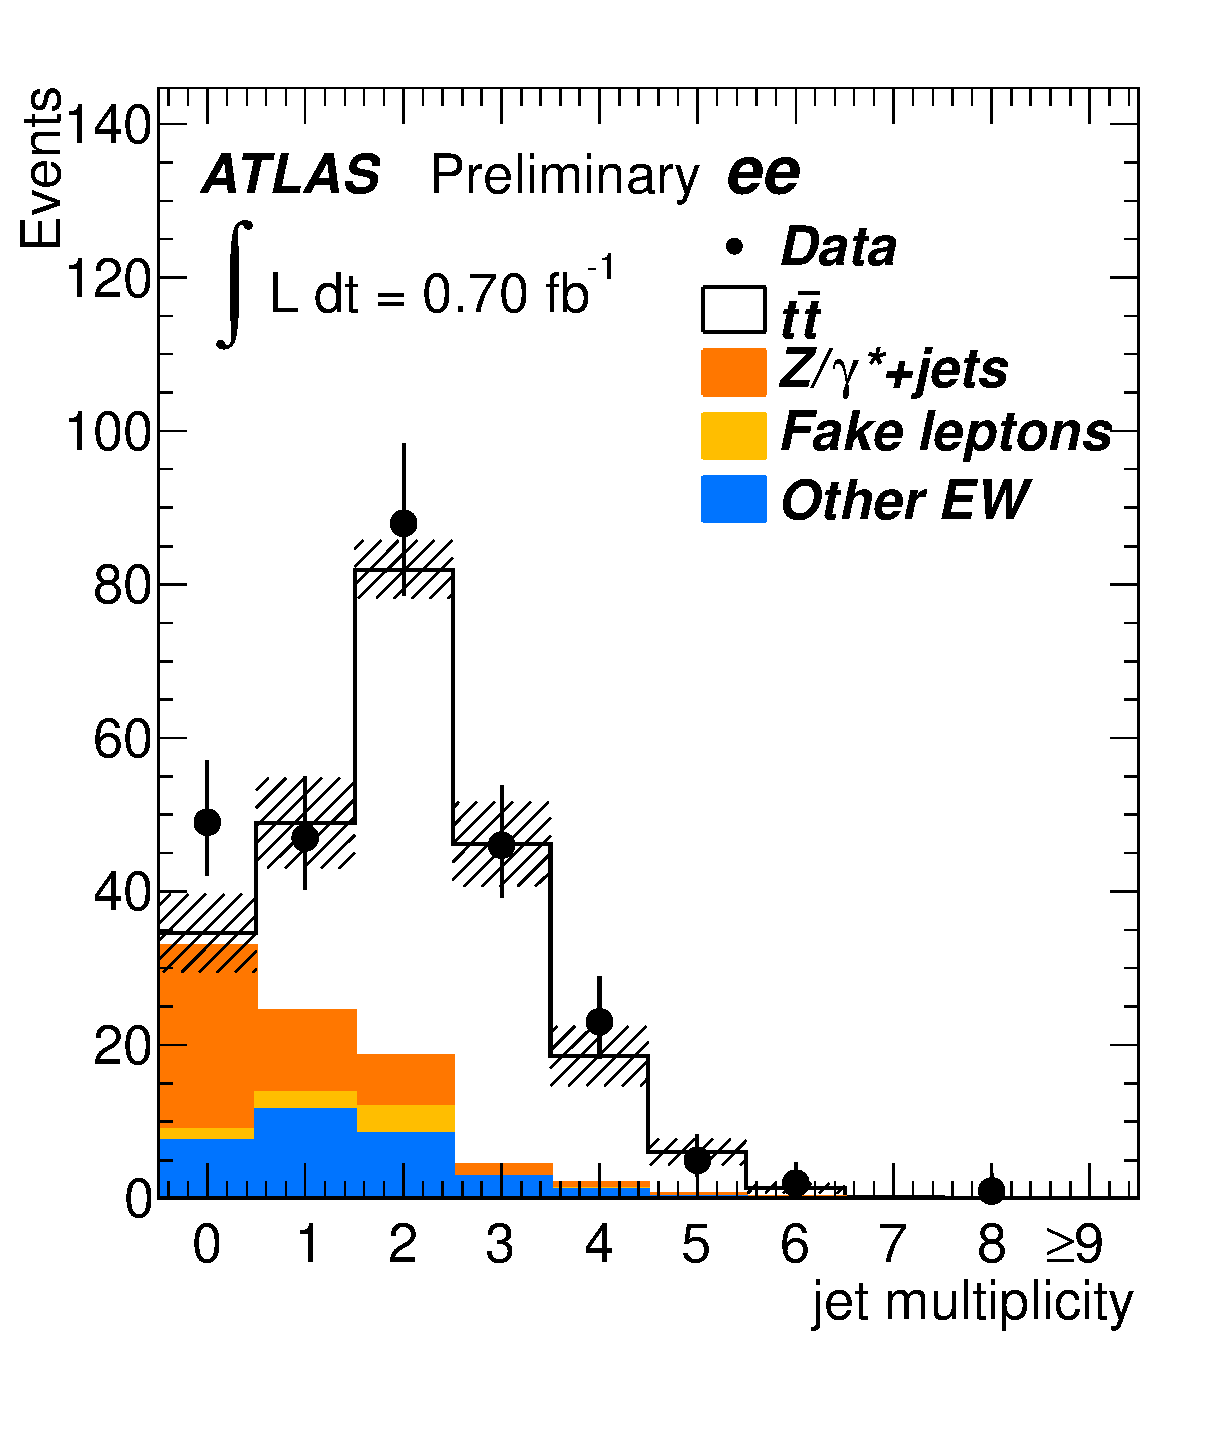
\includegraphics[width=.40\textwidth]{figures/dilep/ee_n_jets} }
    \subfigure[$\mu \mu$]{  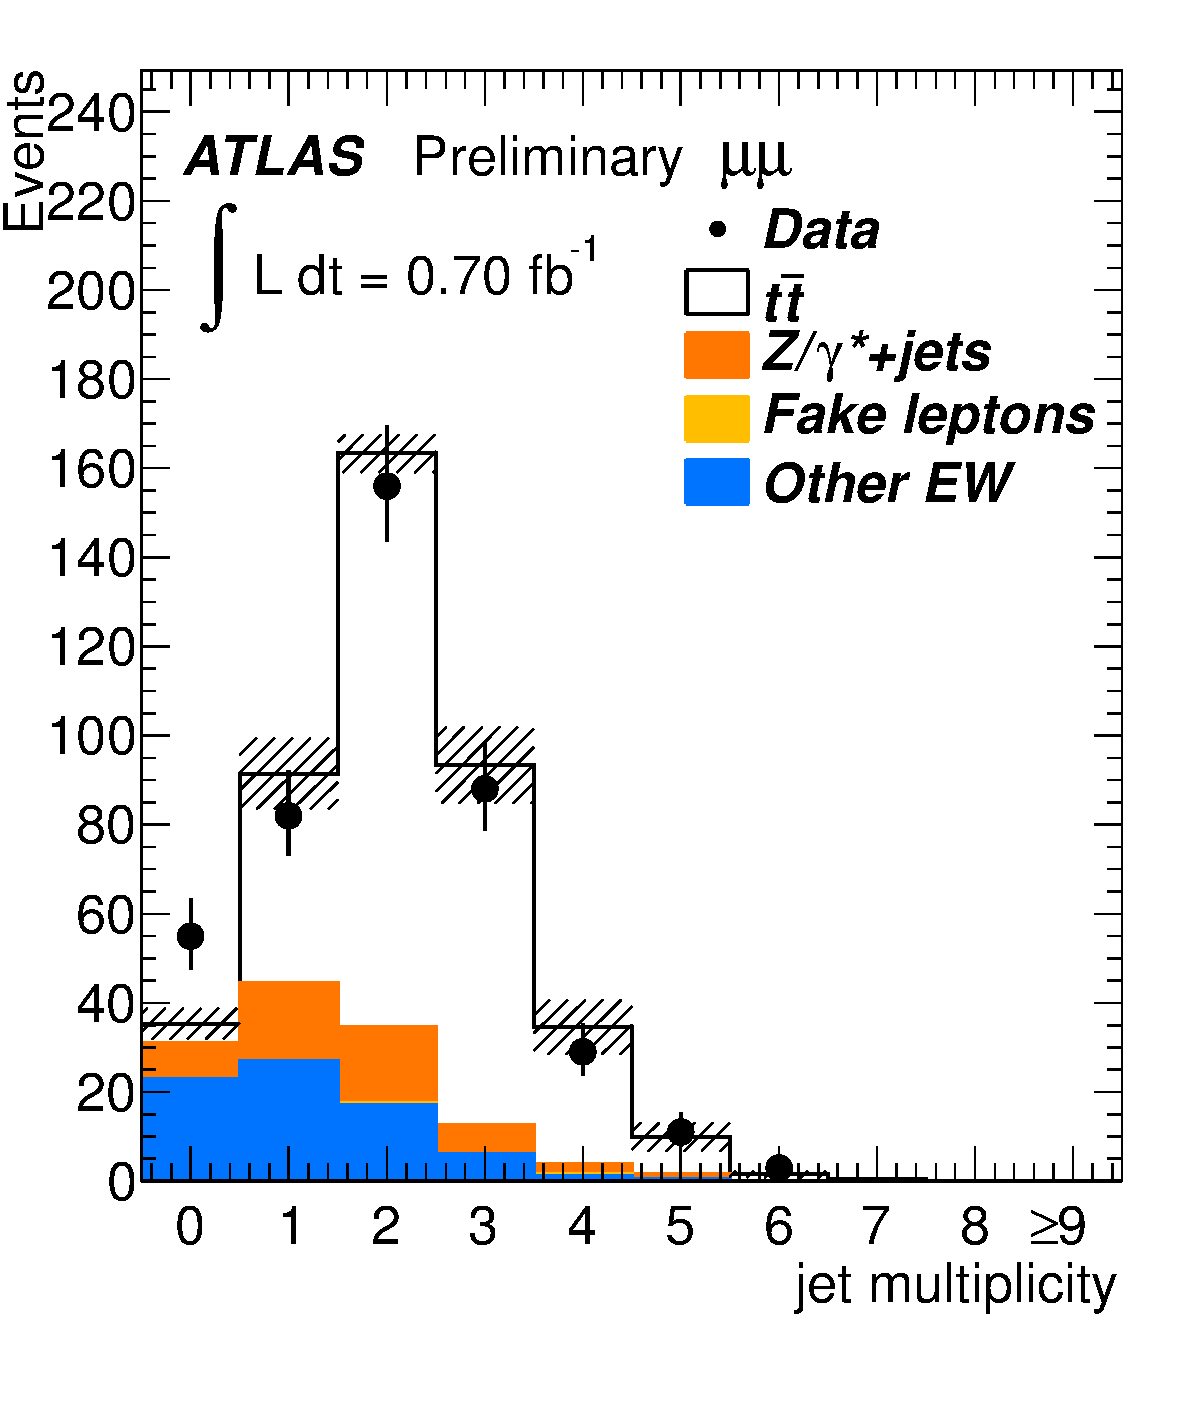
\includegraphics[width=.40\textwidth]{figures/dilep/mm_n_jets} }
    \subfigure[$e \mu$]{    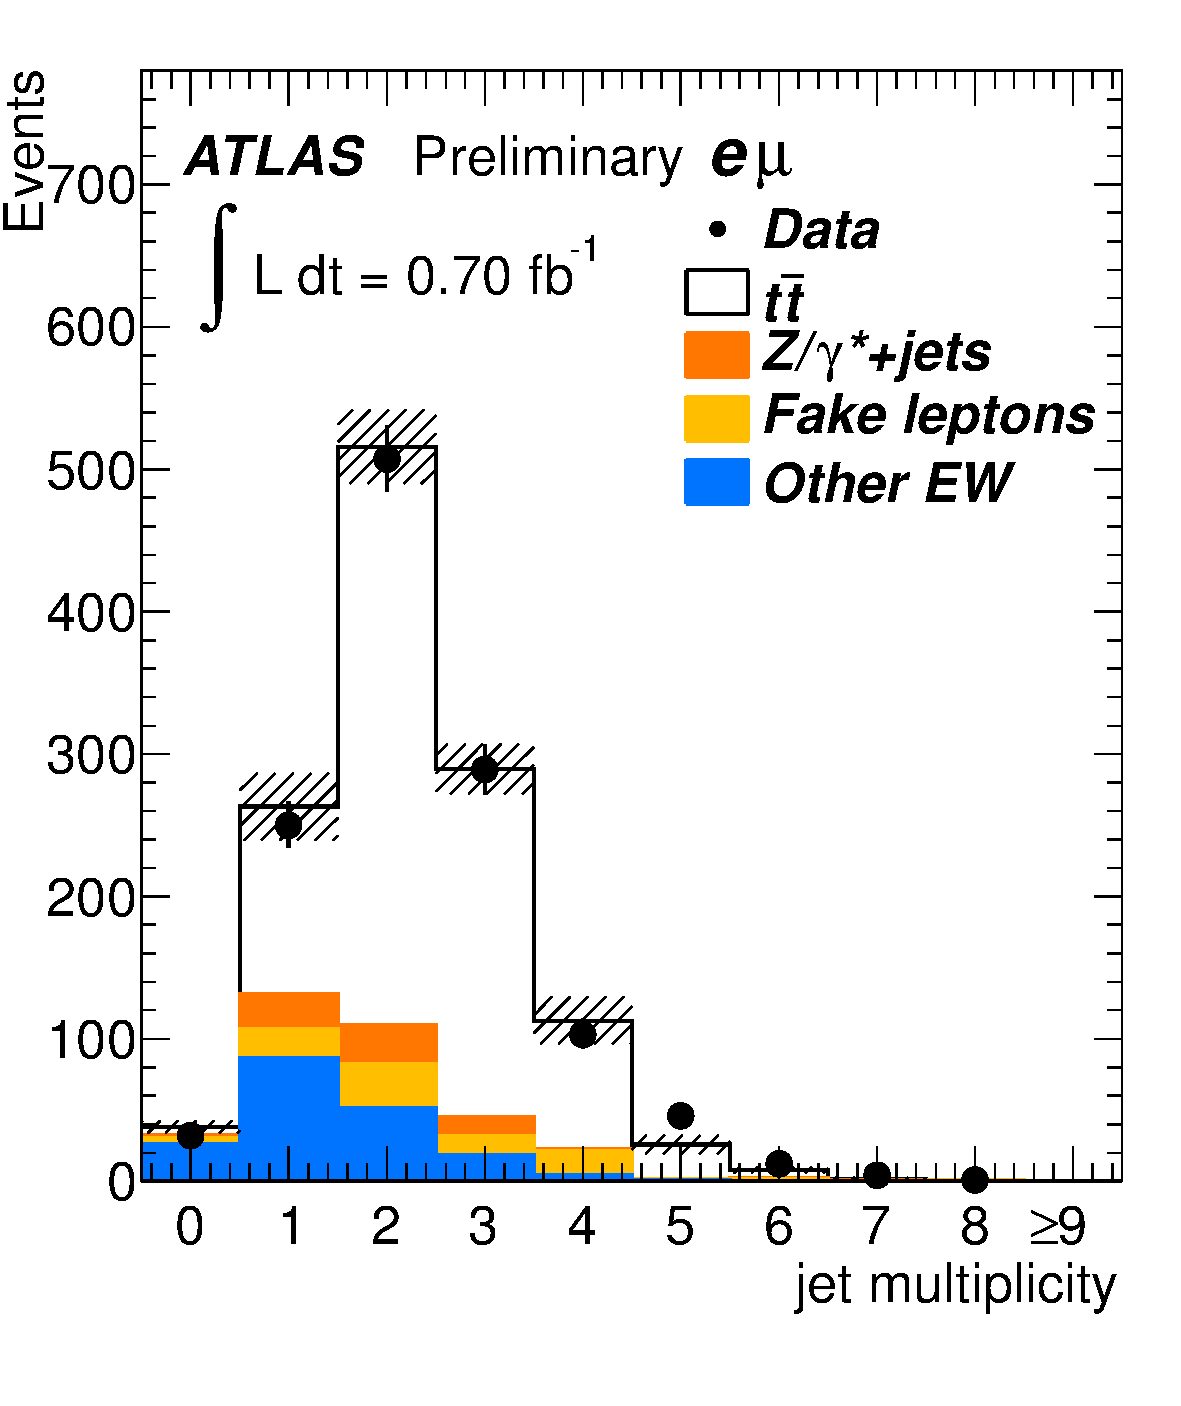
\includegraphics[width=.40\textwidth]{figures/dilep/em_n_jets} }
    \caption{ Jet multiplicity distribution for $ee$, $\mu\mu$, and $e\mu$ events.
      Contributions from diboson and single top-quark events are summarized as `Other EW'.
      Uncertainties shown are statistical and systematic combined.
      The distributions are shown as stacked histograms.}
    \label{f:ll_njets}
  \end{center}
\end{figure}



\begin{figure}[htbp]
  \begin{center}
    \subfigure[$ee$]{       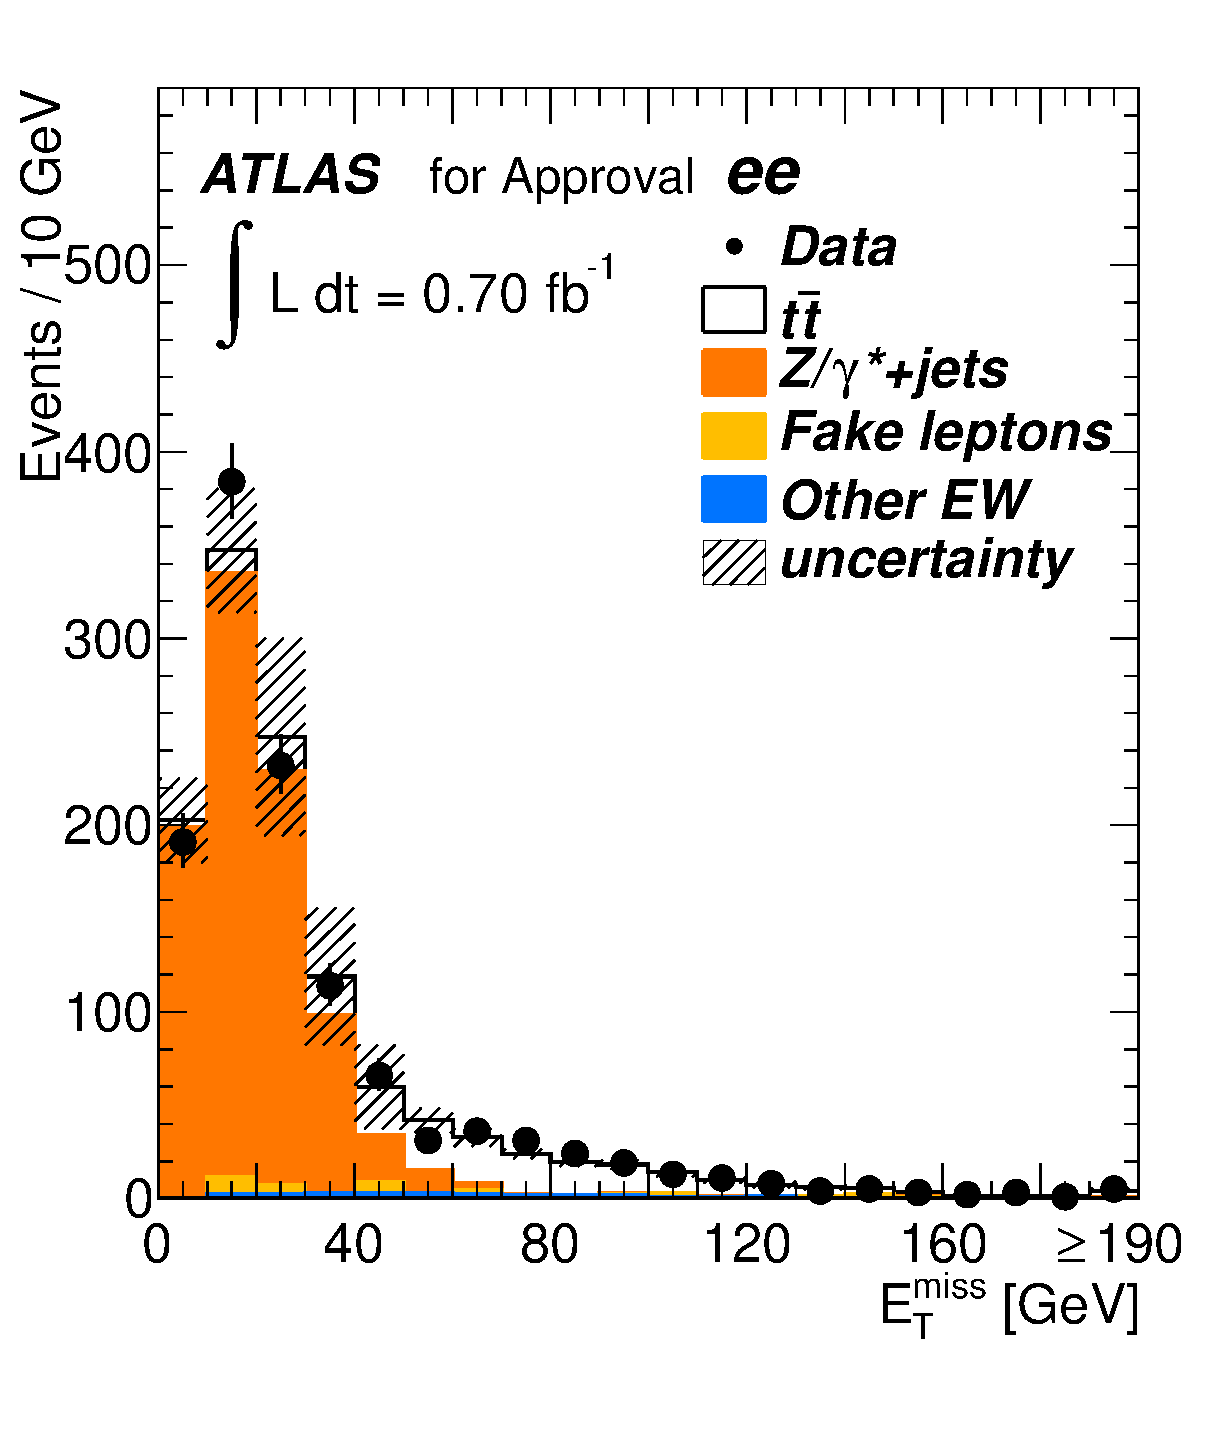
\includegraphics[width=.40\textwidth]{figures/dilep/ee_met} }
    \subfigure[$\mu \mu$]{  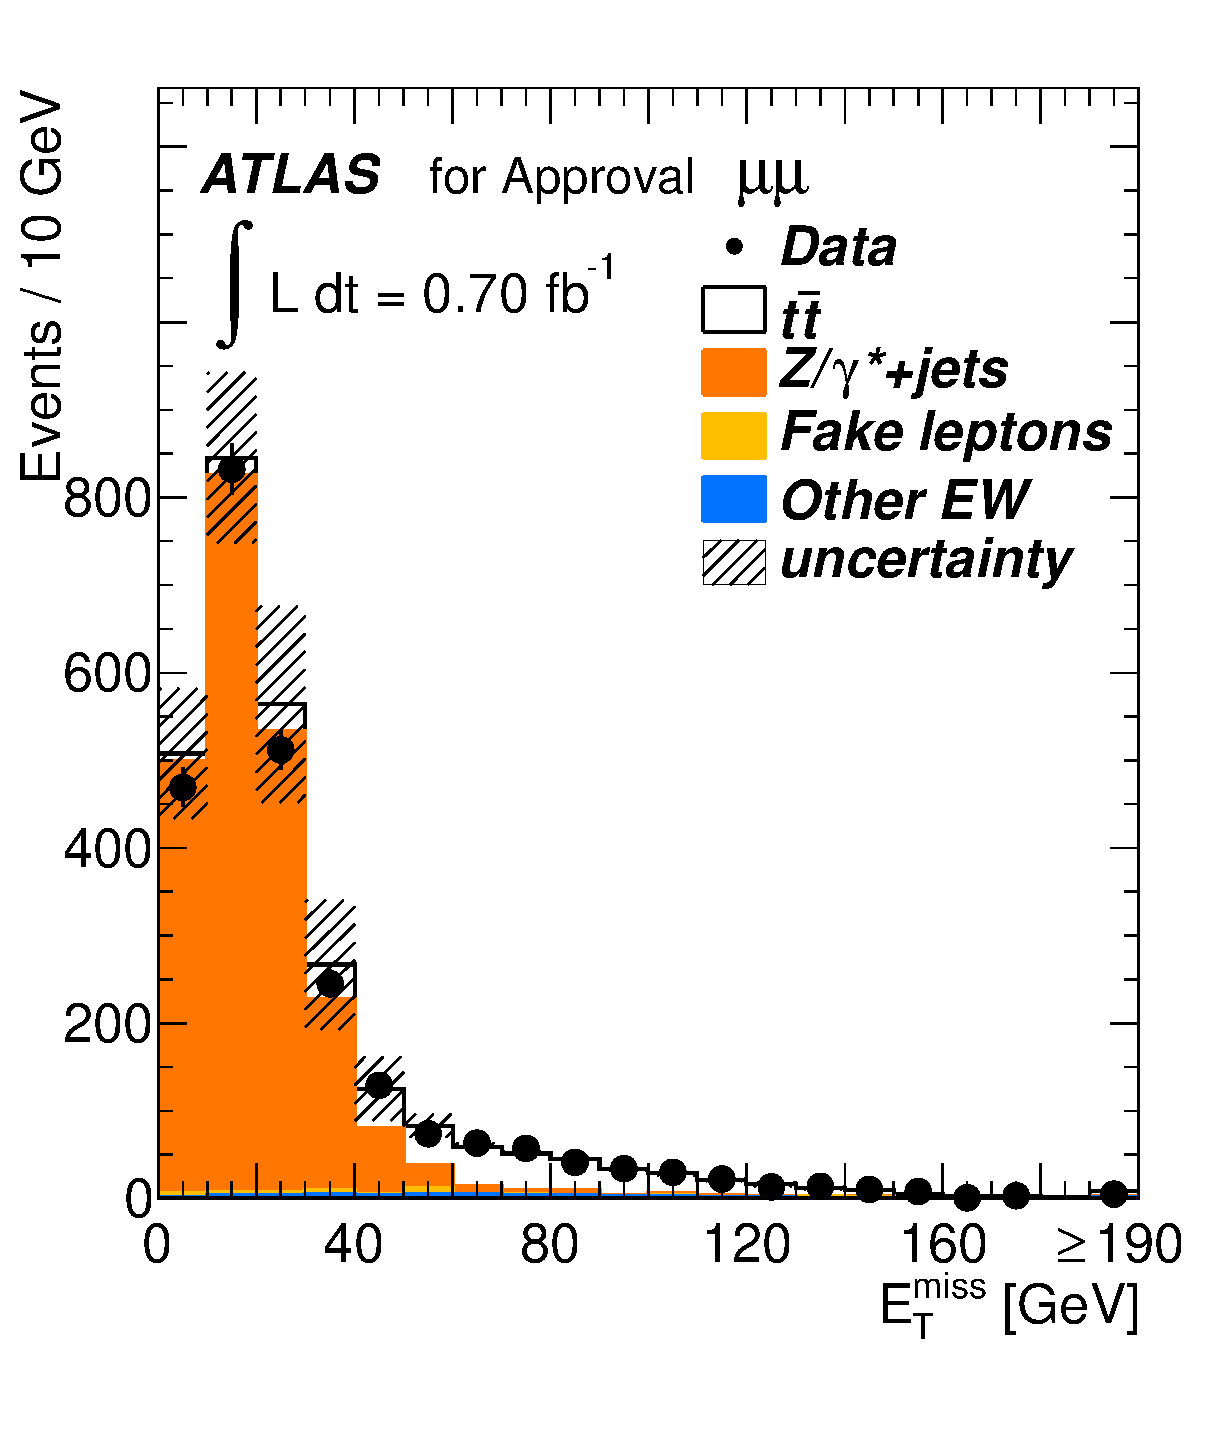
\includegraphics[width=.40\textwidth]{figures/dilep/mm_met} }
    \subfigure[$e \mu$]{    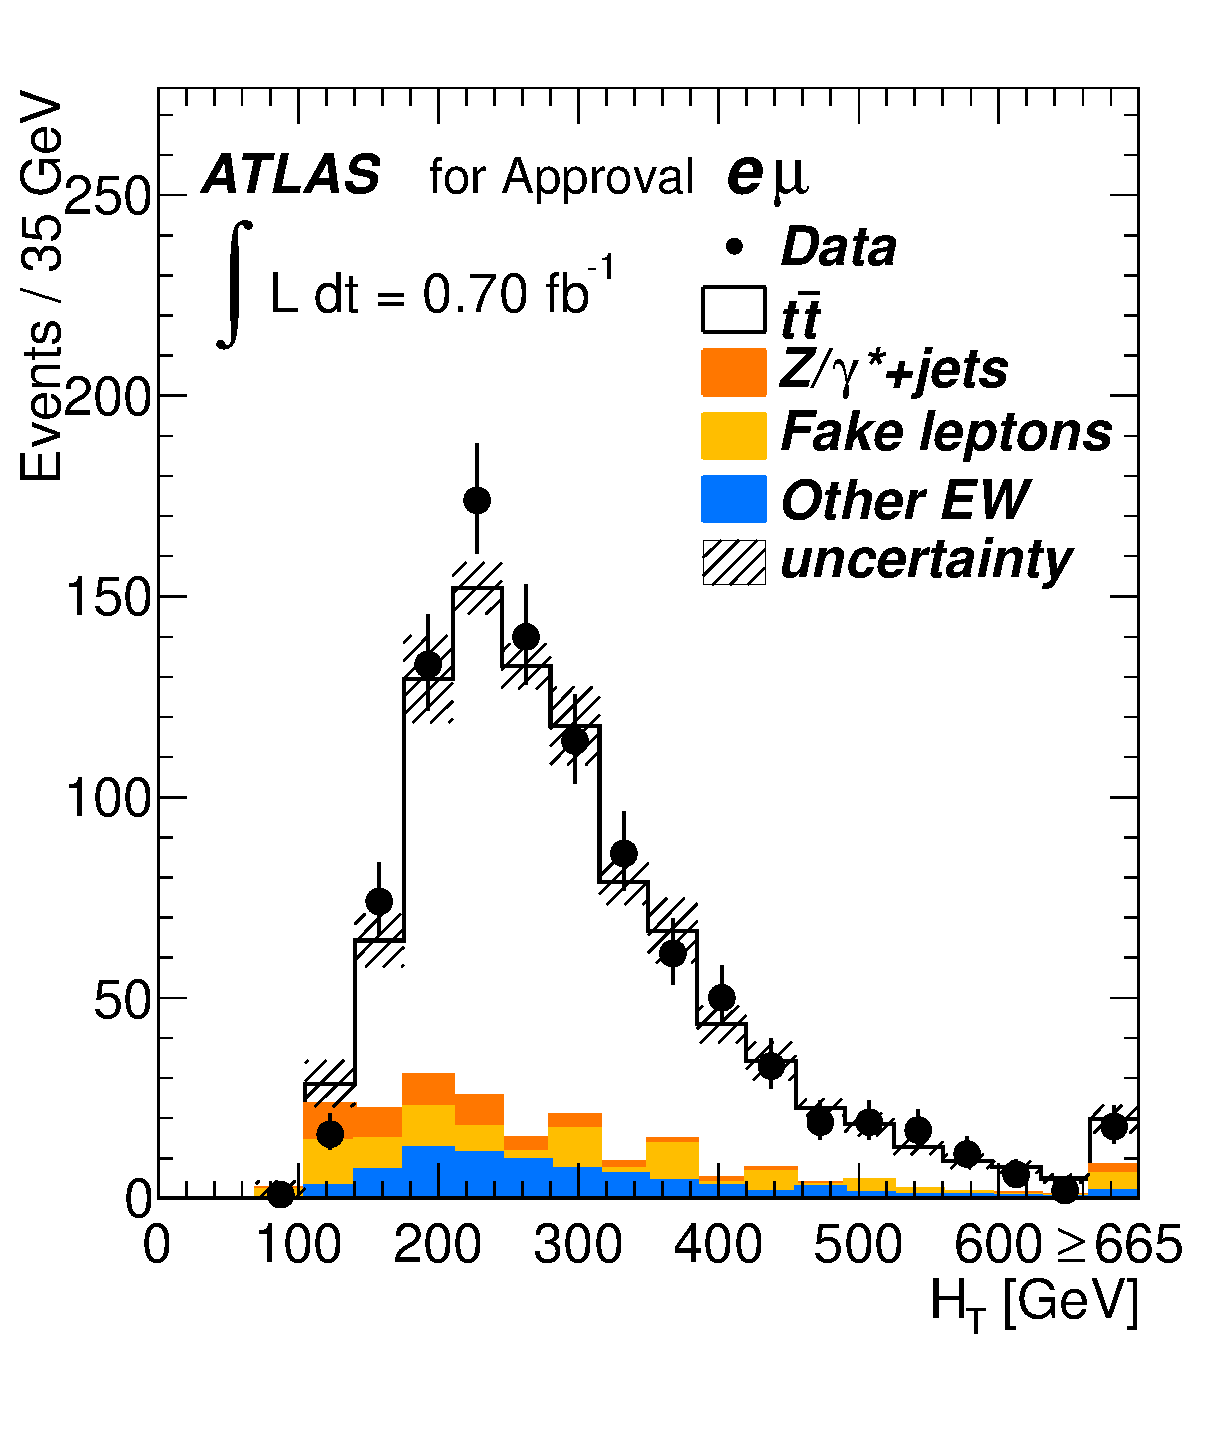
\includegraphics[width=.40\textwidth]{figures/dilep/em_ht} }
    \caption{ Jet multiplicity distribution for $ee$, $\mu\mu$, and $e\mu$ events.
      Contributions from diboson and single top-quark events are summarized as `Other EW'.
      Uncertainties shown are statistical and systematic combined.
      The distributions are shown as stacked histograms.}
    \label{f:ll_njets}
  \end{center}
\end{figure}

%% \begin{figure*}
%%   \centering
%%   \subfigure[]{
%%     \includegraphics[width=0.45\textwidth]{figures/dilep/pretag_combined_nJets}
%%   }
%%   \subfigure[]{
%%     \includegraphics[width=0.45\textwidth]{figures/dilep/btag_preTagFinalJetnJetJetProbTaggedJet_all_ATLAS2}
%%   }
%%   \caption{ (a) Jet multiplicity distribution for
%%     $ee$+$\mu\mu$+$e\mu$+$e$TL+$\mu$TL events without a $b$-tagging requirement. (b)
%%     Multiplicity distribution of $b$-tagged jets in the $ee$+$\mu\mu$+$e\mu$ channels. Contributions from diboson and
%%     single top-quark events are summarized as `Other EW'. The
%%     events in (b) are not a simple subset of those in (a) because the
%%     event selections for the $b$-tag and non-$b$-tag analyses differ.
%%     Uncertainties shown are statistical and systematic combined. The
%%     distributions are shown as stacked histograms.}
%%   \label{f:ll_njets}
%% \end{figure*}

%% \begin{figure*}
%%   \centering
%%   \subfigure[]{
%%     \includegraphics[width=0.41\textwidth]{figures/dilep/pretag_combined_Met_log}
%%   }
%%   \subfigure[]{
%%     \includegraphics[width=0.41\textwidth]{figures/dilep/btag_jetProbTaggedInSRMEt_all_logscale_ATLAS2}
%%   }
%%   \caption{
%%     The $\met$ distribution in the signal region for (a) the five
%%     non-$b$-tag channels combined and, (b) the three $b$-tagged channels
%%     combined.  Contributions from diboson and single top-quark events
%%     are summarized as `Other EW'. Uncertainties shown are statistical
%%     and systematic combined. The last bin in each figure is an
%%     overflow bin, including all events above 190 GeV. The distributions
%%     are shown as stacked histograms.}
%%   \label{f:ll_met_ht}
%% \end{figure*}


The cross-section results are obtained with a profile likelihood
technique, as described in Ref.~\cite{ATL-CONF-2011-034}. The
branching fraction for $t\rightarrow Wb$ is taken to be 100\% and
the acceptance is calculated for a top mass of 172.5 GeV.

%% The top-quark pair production cross section measured by combining
%% the seven channels, the non-$b$-tagged $ee$, $\mu\mu$, $e\mu$, $e$TL
%% and $\mu$TL and the exclusive $b$-tagged $ee$ and $\mu\mu$, is
%% \[
%% \sigmattbar=\mathrm{}\xsecctot \xseccstat
%% \mathrm{(stat.)}\xseccsyst \mathrm{(syst.)} \xsecclumi
%% \mathrm{(lumi.)}~\rm pb.
%% \]

Figure~\ref{fig:XsecSummary} summarizes the cross sections
for the individual channels,  and the combination of the non-$b$-tag and
the exclusive $b$-tagged data sets.

\begin{figure}[!h]
\centering
\includegraphics[width=0.5\textwidth]{figures/dilep/summary_dilep_atlforaproval}
    \caption{Summary of the individual cross section measurements and the combination of non-$b$-tag and
    exclusive $b$-tagged results. The vertical dashed line and yellow band are the approximate NNLO theory calculation and its uncertainty.}
    \label{fig:XsecSummary}
\end{figure}

The measured cross section is in good agreement with a similar
measurement made with 2010 data by the CMS
collaboration~\cite{Chatrchyan:2011nb}, %with 2010 ATLAS measurements
with an ATLAS measurement in the dilepton channel with earlier
data~\cite{ATL-CONF-2011-034}, and with the SM
prediction of
$165\pmasym{11}{16}$~pb. Compared to the earlier ATLAS measurement
in the dilepton channel, the statistical uncertainty of the
measurement has been reduced by a factor of four with the addition
of more data, and a small reduction in the systematic uncertainty,
which now dominates, has been achieved.



\subsection{Results}
\label{s:summary}


The top-quark pair production cross section is measured using  events
selected by requiring two oppositely-charged lepton candidates, at least two
additional jets and missing transverse energy.
%A measurement is also made requiring one of the jets to be identified as a $b$-quark jet.

The top-quark pair production cross section measured without
$b$-tagging is
\[
\sigmattbar=\mathrm{}\xsectot \xsecstat \mathrm{(stat.)}\xsecsyst \mathrm{(syst.)} \xseclumi \mathrm{(lumi.)}~\rm pb.
\]
Using $b$-tagging, the cross section is
\[
\sigmattbar=\mathrm{}\xsecbtot \xsecbstat  \mathrm{(stat.)}\xsecbsyst \mathrm{(syst.)} \xsecblumi  \mathrm{(lumi.)}~\rm pb.
\]
These results have been cross checked with other techniques,
confirming their robustness.


%% Finally the combination of the non-$b$-tagged and the exclusive $b$-tagged
%% data sets yields
%% \[
%% \sigmattbar=\mathrm{}\xsecctot \xseccstat  \mathrm{(stat.)}\xseccsyst \mathrm{(syst.)} \xsecclumi  \mathrm{(lumi.)}~\rm pb.
%% \]

The cross-section results are summarized in Fig.~\ref{fig:XsecSummary}.
%Along with the cross-checks, the kinematic properties of the selected events
%have been found to be compatible with a heavy particle pair where each particle decays into a jet, lepton and neutrino~\cite{ATL-CONF-2011-034}.

\begin{figure}[!h]
\centering
%    \includegraphics[width=0.5\textwidth]{f/summary_dilepDetail_atlprelim}
\includegraphics[width=0.5\textwidth]{figures/dilep/summary_dilepDetail}
    \caption{ Cross section summary.}
    \label{fig:XsecSummary}
\end{figure}

The measured cross sections are in good agreement with a similar
measurement made with 2010 data by the CMS
collaboration~\cite{Chatrchyan:2011nb}, with 2010 ATLAS measurements
made in the complementary lepton+jets
channels~\cite{ATLAS-CONF-2011-023,ATLAS-CONF-2011-035}, with an
ATLAS measurement in the dilepton channel with earlier
data~~\cite{ATL-CONF-2011-034}, and with the SM prediction of
$165\pmasym{11}{16}$~pb. The agreement between the measurements with
and without $b$-tagging requirements confirms that the candidate
events arise from top quark pair production.
%Together,
%they set the stage for top production and decay studies with an
%order of magnitude more data that will be collected at the LHC in
%the near future.


\def \htjet {H_{\mathrm{T}}}
\def \pt {p_{\mathrm{T}}}
%% \def \et {E_{\mathrm{T}}}
%% %\def \met {\not\!\!{E_{\mathrm{T}}}}
%% \def \met {E_{\mathrm{T}}^{\mathrm{miss}}}

%% \newcommand{\ie}{{\it i.e.}~}
%% \newcommand{\wj}{{\tt W+jets}~}
%% \newcommand{\zj}{{\tt Z+jets}~}
%% \newcommand{\lumi}{$\mathcal{L}$~}
%% %\newcommand{\ttbar}{$t\bar{t}$~}
\newcommand{\mj}{multi-jet~}
%% \newcommand{\abcd}{{\tt ABCD~}}

%% \newcommand{\epsb}{$\epsilon_{B}~$}
%% \newcommand{\eps}{$\epsilon_s~$}

\newcommand{\Nb}{${\rm N}_{b}~$}
\newcommand{\Nc}{${\rm N}_{c}~$}
\newcommand{\Na}{${\rm N}_{a}~$}
\newcommand{\Nd}{${\rm N}_{d}~$}

\newcommand{\bb}{$n_{b}~$}
\newcommand{\bc}{$n_{c}~$}
\newcommand{\ba}{$n_{a}~$}
\newcommand{\bd}{$n_{d}~$}

%% \newcommand{\Sb}{$s_{B}~$}
%% \newcommand{\btt}{\ttbar background~}
%% \newcommand{\dib}{di-bosons~}
%% \newcommand{\st}{single top~}

\newcommand{\Ar}{{\tt A}}
\newcommand{\Br}{{\tt B}}
\newcommand{\Cr}{{\tt C}}
\newcommand{\Dr}{{\tt D}}


\section{All Hadronic}

% https://svnweb.cern.ch/trac/atlasphys/browser/Physics/Top/Summer11/INT_XS_allhad/conf.tex
%https://atlas.web.cern.ch/Atlas/GROUPS/PHYSICS/CONFNOTES/ATLAS-CONF-2011-140/


%% The data used in this analysis were collected during the 2011 data taking period with 
%% $pp$ collisions at $\sqrt{s}=$~7~TeV. All data used in this analysis were recorded with 
%% stable beam conditions with all relevant subsystems fully operational and represent a 
%% total integrated luminosity of 1.02~$\ifb$ with an uncertainty of 3.7\%~\cite{ref:lum}. 
%% The data sample has been collected with un-prescaled \mj triggers, which for most
%% of the period correspond to a trigger that requires five jets with $|\eta| <$~3.2 and 
%% $\et$~$>$~10 GeV at Level-1, 25~GeV at Level-2 and 30~GeV at the Event Filter~\cite{ref:JetTrigger}. 
%% For our baseline event selection a requirement of at least five offline jets with $\et >$~55~GeV is used, for this cut 
%% the single jet trigger efficiency is 90\%, the plateau of 100\% is reached only for jets with $\et >$~60~GeV.


%\subsection{Introduction}

In this section, we describe a final measurement of the top-quark pair-production cross-section using the final state topology where both $W$ bosons decay hadronically, 
which we refer to as the all-hadronic final state.
This channel has the advantage of a large brancing ratio of 46\%~\cite{ref:PDG}.
However, because the final state topology contains no leptons, it suffers from a large QCD background.
To separate the signal from this QCD background, this analysis exploits both topological characteristics
of the final state and uses $b$-jet requirements to reduce backgrounds.
Finally, a discriminating variable based on the details of the $\ttbar$ topology is used to measure the cross-section.
This analysis was performed using an integrated luminosity of 1.02~$\ifb$ of data taken in 2011~\cite{ref:ATLAS}.

%% To isolate the $\ttbar$ signal,
%%  several kinematic and topological characteristics 
%% of the signal can be exploited together with $b$-jet identification requirements 
%% based on a secondary-vertex-based algorithm ($b$-tagging). 

%% The reconstructed object 
%% definitions and event selections are described in Section~\ref{sec:obj}. 
%% After preselection, the Event Mixing algorithm, described in Section~\ref{sec:bkg},
%% is used to reconstruct the mass $\chi^2$ background distribution built on the hypothesis of a
%%  \ttbar~final state and to measure the cross-section as described in Section~\ref{sec:xsec}. 
%% As cross check of the Event Mixing analysis, the results produced with the ABCD method are described in Section~\ref{sec:abcd}.
%% A review of the sources of systematic uncertainties is given in Section~\ref{sec:sys}, and finally the summary can be found 
%% in Section~\ref{sec:sum}.

\subsection{Detector, data and simulated samples}
\label{sec:datasample}


The data collected for this analysis was selected using a set of unprescaled multijet triggers.
For the majority of the data-taking period, these triggers required five jets all with 
$|\eta| <$~3.2 and $\et$~$>$~30~GeV~\cite{ref:JetTrigger}.

%For our baseline event selection a requirement of at least five offline jets with $\et >$~55~GeV is used, for this cut 
%the single jet trigger efficiency is 90\%, the plateau of 100\% is reached only for jets with $\et >$~60~GeV.

%% The data sample has been collected with un-prescaled \mj triggers, which for most
%% of the period correspond to a trigger that requires five jets with $|\eta| <$~3.2 and 
%% $\et$~$>$~10 GeV at Level-1, 25~GeV at Level-2 and 30~GeV at the Event Filter~\cite{ref:JetTrigger}. 
%% For our baseline event selection a requirement of at least five offline jets with $\et >$~55~GeV is used, for this cut 
%% the single jet trigger efficiency is 90\%, the plateau of 100\% is reached only for jets with $\et >$~60~GeV.


The $\ttbar$ signal was modeled using Monte Carlo simulation generated using the {\sc MC@NLO}~v3.41~\cite{FRI-0201} 
generator with PDF set CTEQ6.6~\cite{Nadolsky:2008zw}, assuming a top quark mass of 172.5~GeV.
To validate this model and to estimate the size of certain systematic uncertainties, an alternate set of events were 
generated using the {\sc POWHEG}~\cite{FRI-0701} generator.
Due to the large uncertainties that result from the generation of QCD events with many partons in the final state, 
a data-driven technique was used to estimate QCD backgrounds.
We assume that other types of background of neglegable in this analysis.

%% \noindent The modelling of $\ttbar$ signal and its associated selection efficiency is derived from Monte Carlo (MC).
%% For the MC generation of the $t\bar{t}$ signal, the 
%% the {\sc MC@NLO}~v3.41~\cite{FRI-0201} generator with PDF set CTEQ6.6~\cite{Nadolsky:2008zw} was used to 
%% tune the selection criteria and build a signal template to fit the data, 
%% assuming a top quark mass of 172.5~GeV. The {\sc POWHEG}~\cite{FRI-0701} generator
%% was used as an alternative to study the systematic uncertainty due to the signal modelling.
%% \noindent The generated events were processed through the full ATLAS detector 
%% simulation based on {\sc GEANT4}~\cite{AGO-0301} followed by the trigger and 
%% offline reconstruction. Due to the large uncertainty in the QCD \mj cross-section prediction, 
%% we employed a data-driven technique described in Section~\ref{sec:bkg} to estimate 
%% the background. The cross-check analysis requires the use of a simulated set of standard background
%% processes ({\it W}+jets, {\it Z}+jets, single top and dibosons)~\cite{FIRSTOPPAPER}.



\def \pt {p_{\mathrm{T}}}

\subsection{Object definition and event selection}
\label{sec:obj}

%\subsubsection{Jets}

The accurate reconstruction of jets is crucial for this analysis,
as they are the only physical objects that appear in the final state.
However, the reconstruction of leptons is necessary for the purpose 
of vetoing them in the final state.
Jets are reconstructed with the anti-$k_{\mathrm{t}}$ algorithm~\cite{Cacciari200657,Cacciari:2008gp} with a distance parameter $R=0.4$. %. using the FastJet package~\cite{ref:FastJet}. 
The energy of jets is calibrated based on $\pt$ and $\eta$-dependent corrections.
Jets within $\Delta R$=0.2 to an electron are rejected.
For this step, electrons are required to satisfy the standard set of cuts, including tight track quality and shower shape, isolation, and they must have $p_{\mathrm{T}}>20$~GeV and $|\eta_{\mathrm{cluster}}|<2.47$~\cite{ATLAS-CONF-2011-100}.
Finally, selected jets are required to have $\pt$~$>$~20~GeV and $|\eta|$~$<$~4.5~\cite{ref:jets,ref:jessys}.

%% The inputs to the jet reconstruction 
%% are topological clusters calibrated at the electromagnetic (EM) scale. 
%% A jet energy calibration based on a $\pt$- and $\eta$-dependent correction 
%% derived from MC simulation is applied. If a jet is closer than $\Delta R$=0.2 to an electron 
%% identified as discussed below, the jet is removed from consideration to 
%% avoid double-counting. Only jets with $\pt$~$>$~20~GeV and $|\eta|$~$<$~4.5 are
%% considered in this analysis. A detailed description of the jet 
%% definition can be found in Refs.~\cite{ref:jets,ref:jessys}.

%\subsubsection{Identification of $b$-jets}

To reduce the contamination from QCD background, the all hadronic analysis uses $b$-tagging to classify jets originating from $b$ quarks.
Jets are tagged using a neural-network algorithm that combines features that are generated by two separate algorithms.
The first of these, called JetFitter, is based on the secondary-vertex of the jet as well as the topology of secondary decays within the jet~\cite{ATLAS-CONF-2011-102}.
The second tagger, known as ID3D, generates a likelihood discriminant based on the impact parameters of tracks associated with the jetthe transverse and longitudinal impact parameters ~\cite{ATLAS-CONF-2011-102}.
The cut on the output of the neural network is tuned to classify real $b$-jets originating from $\ttbar$ events with 60\% efficiency.

%% The identification of jets originating from a $b$-quark is performed using a 
%% secondary-vertex-based tagging algorithm, called JetFitter~\cite{ATLAS-CONF-2011-102}.
%% JetFitter exploits the topology of weak $b$- and $c$-hadron decays inside the jet.
%% A Kalman filter is used to find a common line on which the primary vertex and the $b$- and $c$-hadron decay vertices
%% lie, as well as their positions on this line, giving an approximated flight path for the $b$-hadron.
%% With this approach, the $b$- and $c$-hadron vertices are not necessarily merged, even when only a single
%% track is attached to each of them. The discrimination between $b$-, $c$- and light-jets
%% is based on a likelihood using the masses, momenta, flight-length significances, and track multiplicities
%% of the reconstructed vertices as inputs. 
%% To further increase the flavour discrimination power, a second $b$-tagger (IP3D)~\cite{ATLAS-CONF-2011-102} is run,  
%% that does not attempt to directly reconstruct decay vertices.
%% Instead, this tagger uses the transverse and the longitudinal impact parameter significances of each
%% track within the jet to determine a likelihood  that the jet originates from a $b$-quark. 
%%  The IP3D and JetFitter tagger results are combined using an 
%% artificial neural network to determine a single discriminant variable (JetFitterCombNN) that
%% is used to make tagging decisions.
%% For this analysis we tune this cut to accept $b$-jets with approximately 60\% efficiency on simulated $\ttbar$ events. 
%% This corresponds to a light jet rejection factor of about 350.

%% \subsubsection{Leptons and missing transverse energy}
%% The all-hadronic $t\bar{t}$ channel nominally has six jets and does not contain 
%% intrinsic missing transverse energy ($\met$) or isolated leptons in the final state. 
%% Therefore, to avoid overlap with other $t\bar{t}$ cross-section measurements and to reduce the 
%% background due to events containing $W$ bosons that decay leptonically, a veto against 
%% high-$\pt$ isolated leptons 
%% and significant $\met$ is applied. The leptons and $\met$ used for this veto are defined 
%% according to the following criteria:
%% \begin{itemize}
%% \item Electron candidates are required to pass a standard tight 
%%       electron selection as defined in Ref.~\cite{ATLAS-CONF-2011-100}, with 
%%       $p_{\mathrm{T}}>20$~GeV and $|\eta_{\mathrm{cluster}}|<2.47$, 
%%       but excluding the barrel-endcap calorimeter transition region at $1.37<|\eta|<1.52$. In order to suppress background from hadrons faking an electron signature, electrons from heavy-flavour decays and photon conversions, 
%%       an isolation criteria is applied to the selected electrons. The selected electron is required to have little jet activity in the space surrounding its direction ($\Delta R$~$<$~0.2).
%%       The energy measured in a cone of $\Delta R$~$<$~0.2 centered around the electron direction  is required to be below 3.5~GeV.

%% \item Muons are reconstructed by combining the measurements of the tracks
%%       detected in the muon spectrometer with those of the associated
%%       track in the inner detector~\cite{ATLAS-CONF-2011-100}. 
%%       Good muon candidates 
%%       are selected by requiring $p_{\mathrm{T}}>$~20~GeV and $|\eta|<$~2.5. 
%%       An additional isolation requirement is applied to select only muons 
%%       with both a $p_{\mathrm{T}}$ sum of calorimeter clusters and of tracks in 
%%       a cone with $R=0.3$ around the muon candidate of less than 4~GeV.

The missing transverse energy using the event selection of this analysis is constructed using topological clusters that have been corrected according to the object that they are associated with.
To further separate signal events from background, this analysis considers a quantity known as the missing energy significance, which measures the relative amount of missing energy in units of the standard deviation of the size of fake missing energy, which mostly comes from calrimeter mismeasurement.
The missing transverse energy significance is defined as $\met/ \sqrt{\htjet}$, where $\htjet$ is the scalar sum of the transverse momentum of all jets in the event.


%% The missing transverse energy, $\met$, is an object-based
%% definition calculated from topological clusters calibrated at the EM scale and corrected
%% according to the energy scale of the associated object.
%%       Calorimeter clusters not associated to any high $p_T$ object are included at the EM scale and
%%       corrections for the muon/electron candidates are applied~\cite{ref:jets,ref:jessys}. 

%================================================================================
\subsubsection{Event selection}
\label{subsec:EvSel}
%================================================================================

Events are first required to satisfy the multijet trigger algorithms described above.
From that selection of candidiate events, the signal region is obtained by requiring no leptons with $p_{\rm T}$~$>$~20~GeV, 
five or more jets with $p_{\rm T}$~$>$~55~GeV, and at least one additional jet with $p_{\rm T}$~$>$~30~GeV.
At least two of the selected jets must satisfy the $b$-tagging requirement.
In addition, the event must have a missing energy significance < 3 to remove electroweak events and events with badly mismeasured jets.
Finally, there is a topological requirement on the two tagged $b$-jets which must be separated by $\Delta R(b,\bar{b}) =$~1.2, 
which attempts to remove $b\bar{b}$ pairs not originating from the decay of $\ttbar$.

%% \Events are selected by first requiring that the trigger signature described in Section~\ref{sec:datasample} is satisfied.
%% A series of kinematic cuts are applied to the events to define the signal region. Events are first required to have:
%% \begin{itemize}
%% \item no isolated lepton with $p_{\rm T}$~$>$~20~GeV;
%% \item at least five jets with $p_{\rm T}$~$>$~55~GeV; % and $|\eta|<4.5$;
%% \item at least six jets with $p_{\rm T}$~$>$~30~GeV. Additional jets are counted for the jet multiplicity if they satisfy $p_{\rm T}$~$>$~20~GeV. %for each additional jet;% all of them within  $|\eta|<4.5$;
%% %\item all jets with $|\eta|<4.5$;
%% \item at least two of the selected jets should be $b$-tagged by the JetFitterCombNN algorithm and have a $p_{\rm T}$~$>$~20~GeV and $|\eta|<2.5$;
%% \item a transverse missing energy significance  $\met/ \sqrt{\htjet} < 3$, where $\htjet$ is the scalar sum of the transverse momentum of all jets in the event, to ensure the observed $\met$ is not due to poorly reconstructed jets;
%% \item a minimum distance between the two $b$-tagged jets $\Delta R(b,\bar{b}) =$~1.2, to remove $b\bar{b}$ pairs originating from gluon splitting.
%% \end{itemize}

%% \noindent The large values for the jet $p_{\rm T}$ cut, 55~GeV on the fifth jet $p_{\rm T}$, is due to the necessity of selecting events that are near the plateau 
%% of the \mj trigger efficiency turn-on curve. The lepton veto and $\met$ 
%% significance cuts are used to reject events from other electroweak processes. 
%% After preselection, 6114 data events are left. For the simulated signal sample,
%% these preselection requirements give a signal efficiency of 1.1\%.



\subsection{Background modeling}
\label{sec:bkg}
\noindent

The most crucial task in this analysis is the proper modeling of the QCD background.
This analysis uses a data-driven tecnique to estimate the shape of this background by measuring the distribution of QCD in control regions
and extrapolating from those control regions to the signal region.
This technique used for extrapolation, which has been used previously in Ref.\cite{PhysRevD.82.032002},
uses a control regions containing exactly four or five jets, which have very little signal contamination,
and uses the jet number distributions in those regions to reconstruct the QCD jet number distribution
in the signal region.
This process of background estimation, which combines events having lower numbers of jets, is known as the EventMixing technique.

%% SUMMARY OF THE BELOW

%%  \item[a)] Three classes of events are selected: exactly four-jet events, exactly five-jet events and finally events with at least six jets. These event samples are required to have at least two $b$-tagged jets and no isolated lepton as defined in Section \ref{sec:obj}. Five-jet events are selected with the fifth jet $p_{\rm T}$~$>$~55~GeV and pass the five-jet trigger. Four-jet events have to pass the four-jet trigger with a $p_{\rm T}$~$>$~80~GeV. The inclusive six-jet events will be used as donors of low $\pt$ jets. These low $\pt$ jets will be added to the acceptor four-jet or five-jet events to model the inclusive six-jet QCD \mj background in the signal region.

%% \item[b)] For a given acceptor four-jet (five-jet) event, a donor event with at least six jets and similar phase space configuration is identified. This is achieved by constraining the leading jet in the four-jet (five-jet) event to match the $p_{\rm T}$ of the leading jet in the inclusive six-jet sample, within a $|\Delta \pt|<$~1~GeV. Since the leading jet $\pt$ is correlated with the momentum transfer of the hard scatter, this constraint ensures that the phase space for the inclusive six-jet donor event and the acceptor event with four (five) jets have similar characteristics. The common constraint on the phase space for the four-jet (five-jet) and the inclusive six-jet event is  reinforced by constraining the fourth (fifth) jet in the two samples to be close in $\pt$ ( $|\Delta \pt|<$~1~GeV). This additional constraint on the softest jet aims to select an event with similar characteristics on the softest donor jet.

%% \item[c)] In the case of a matching pair of donor and acceptor, the acceptor receives the fifth and softer jets from the donor in the case of an exclusive four-jet acceptor. In the case of an exclusive five-jet event acceptor,  the sixth and softer jets from the inclusive six-jet donor are added. The  four-momenta  of additional jets are not modified by the algorithm.  Attention is paid so that the added softer jets do not overlap with any original jet in the four or five-jet acceptor event. This is ensured by requiring $\Delta R> 0.4$ between each pair of jets. Combinations that fail this overlap constraint are not used.

%% \item[d)] For each exclusive four- or five-jet acceptor event, all the inclusive six-jet events are considered for the mixing. If no matching inclusive six-jet event is found, the four or five-jet acceptor event is discarded from the list. If 
%% there are multiple matches, the acceptor event is used up to five times with different donor jets.

%% In the analysis, the \mj background with at least six jets is modelled by applying the algorithm to the exclusive five-jet QCD \mj data events. Since additional jets could  artificially create missing transverse energy, the transverse missing energy significance requirement, as described in \ref{subsec:EvSel}, is applied before the Event Mixing. 




%% %% The most challenging task related to the extraction of the $\ttbar$~production cross-section in the all-hadronic channel is the estimation of the dominant source of background: QCD \mj production.
%% %% The strategy used in this note consists of using a data-driven procedure to reproduce the shape of the different observables from alternative data samples. This technique, labelled in the following as Event Mixing, was originally developed and successfully used in Ref.\cite{PhysRevD.82.032002} to derive the $\ttbar$ production cross-section.  The modelling of the shape of the different kinematic and topological distributions associated with the QCD \mj background is used to define the $\ttbar$ background hypothesis $\chi^2$ template defined in Section~\ref{sec:xsec}. The latter is used with the signal $\ttbar$ template to extract the contribution of both the $\ttbar$ signal and the QCD \mj background. Other background processes included in the selected data sample are tiny by comparison. The shaping of the final $\chi^2$ distribution by the $b$-tagging efficiency's dependence on jet $p_{\rm T}$ is taken into account since the original sample, from which the background is modelled, contains at least two $b$-tagged jets. These two $b$-tagged jets are used to mimic the $b$-jets coming from real top-quark decays in the signal sample.  

%% \subsubsection{Background modelling}
%% \label{subsec:bkg1}
%% \noindent The principle of the Event Mixing technique is to model a higher jet-multiplicity  \mj sample from a lower jet-multiplicity \mj sample, using a similar selection but depleted of signal events. The method uses a sample with a lower number of jets (exclusive) to model a sample with a larger multiplicity: the target multiplicity is made 
%% up by adding jets to the initial sample.
%% The technique is used to model QCD \mj events with at least six jets from events with a jet-multiplicity equal to exactly four or five. These four or five-jet exclusive events constitute a \mj sample which has a negligible amount of contamination from $\ttbar$~ signal events. In the following, the jet numbering is based on $p_{\rm T}$ ordering. The algorithm proceeds as follows:
%% \begin{itemize}

%%  \item[a)] Three classes of events are selected: exactly four-jet events, exactly five-jet events and finally events with at least six jets. These event samples are required to have at least two $b$-tagged jets and no isolated lepton as defined in Section \ref{sec:obj}. Five-jet events are selected with the fifth jet $p_{\rm T}$~$>$~55~GeV and pass the five-jet trigger. Four-jet events have to pass the four-jet trigger with a $p_{\rm T}$~$>$~80~GeV. The inclusive six-jet events will be used as donors of low $\pt$ jets. These low $\pt$ jets will be added to the acceptor four-jet or five-jet events to model the inclusive six-jet QCD \mj background in the signal region.

%% %% \item[a)] Three classes of jet-multiplicity events are selected: exactly four-jet events, exactly five-jet events and finally events with at least six jets. These event samples are requested to have at least two $b$-tagged jets, and satisfy the selection described previously in section \ref{sec:obj}. The inclusive six-jet events will be used as donors of low $\pt$ jets. These low $\pt$ jets will be added to the acceptor four-jet or five-jet events to model the inclusive six-jet QCD \mj sample in the signal region.

%% \item[b)] For a given acceptor four-jet (five-jet) event, a donor event with at least six jets and similar phase space configuration is identified. This is achieved by constraining the leading jet in the four-jet (five-jet) event to match the $p_{\rm T}$ of the leading jet in the inclusive six-jet sample, within a $|\Delta \pt|<$~1~GeV. Since the leading jet $\pt$ is correlated with the momentum transfer of the hard scatter, this constraint ensures that the phase space for the inclusive six-jet donor event and the acceptor event with four (five) jets have similar characteristics. The common constraint on the phase space for the four-jet (five-jet) and the inclusive six-jet event is  reinforced by constraining the fourth (fifth) jet in the two samples to be close in $\pt$ ( $|\Delta \pt|<$~1~GeV). This additional constraint on the softest jet aims to select an event with similar characteristics on the softest donor jet.

%% %% \item[c)] In the case of a pair of donor (inclusive six-jet events) and acceptor (exclusive four-jet or five-jet events) with similar phase space configuration, the inclusive six-jet QCD events is modeled from the four-jet events one by adding the fifth jet or higher to the original four-jet QCD sample. In the case of a five-jet acceptor event, the sixth and lower jets from the inclusive six-jet sample are added to the original five-jet QCD events. These additional jets four-vectors are not modified by the algorithm.  Caution is paid that the randomly additional softer jets which are added to the exclusive four- (five-) jet events,  do not overlap with any jet from the four or five-jet events. This is ensured by requesting a $\Delta R \geq 0.4$ between the constructed \mj QCD events which is an inclusive six-jet event. Combinations which fail this overlap constraint are vetoed.

%% \item[c)] In the case of a matching pair of donor and acceptor, the acceptor receives the fifth and softer jets from the donor in the case of an exclusive four-jet acceptor. In the case of an exclusive five-jet event acceptor,  the sixth and softer jets from the inclusive six-jet donor are added. The  four-momenta  of additional jets are not modified by the algorithm.  Attention is paid so that the added softer jets do not overlap with any original jet in the four or five-jet acceptor event. This is ensured by requiring $\Delta R> 0.4$ between each pair of jets. Combinations that fail this overlap constraint are not used.

%% \item[d)] For each exclusive four- or five-jet acceptor event, all the inclusive six-jet events are considered for the mixing. If no matching inclusive six-jet event is found, the four or five-jet acceptor event is discarded from the list. If 
%% there are multiple matches, the acceptor event is used up to five times with different donor jets.

%% \end{itemize}
%% %More generally, the procedure described above allows to model an inclusive n-jet from an exclusive m-jet \mj event with m$<$n. 
%% In the analysis, the \mj background with at least six jets is modelled by applying the algorithm to the exclusive five-jet QCD \mj data events. Since additional jets could  artificially create missing transverse energy, the transverse missing energy significance requirement, as described in \ref{subsec:EvSel}, is applied before the Event Mixing. 

% which allow to check the systematics associated to the technique. 

%The algorithm for the mixing is summarised on Figure~\ref{fig:mixingalg.eps}.

%\begin{figure}[h!]
%  \begin{center}
%    \includegraphics[width=0.6\linewidth]{figures/mixingalg.eps} 
%  \end{center}
%  \caption{Algorithm for the QCD \mj background generation procedure.}
%  \label{fig:mixingalg.eps}
%\end{figure} 


%% commented for now -> maybe we uncomment it, with Editorial board (need to redo the plots)
%% One valid concern, is that the Event mixing technique which aims to model a higher order multiplicity \mj sample, with a lower order multiplicity one, could alter the relative contribution of the different production processes to the \mj background. These production processes are the $gg \rightarrow b\bar{b}$ hard scatter which is characterized with a $\Delta R(b\bar{b})$ distribution peaked at $\pi$ and the second process arises from $g\rightarrow b\bar{b}$.  
%% These two concurrent processes relative contribution is found  not to be sensitive to the jet multiplicity as shown on figure \ref{fig:plot_dR456.eps} for the three jet multiplicities, four-, five- and six-jet event multiplicities.
%% \begin{figure}[h!]
%%   \begin{center}
%%     \includegraphics[width=0.6\linewidth]{figures/plot_dR456.eps} 
%%   \end{center}
%%   \caption{$\Delta R(b,\bar{b})$ between the two leading b-jets in the four-jet, five-jet and six-jet \mj sample. The peak near $\pi$  is dominated by the direct production process: $gg \to b\bar{b}$ while the peak at low $\Delta R$  is associated to the gluon splitting $g\to b\bar{b}$ contribution.}
%%   \label{fig:plot_dR456.eps}
%% \end{figure} 

%% \subsubsection{Background validation}

%% The Event Mixing technique was shown to reproduce enriched QCD inclusive six-jet events with an independent event sample. This was done by selecting exclusive five-jet events and inclusive six-jet events triggered with the five-jet trigger signature
%%  described in Section~\ref{sec:datasample} . 
%% The same procedure as described in Section \ref{subsec:bkg1} is applied, except that the events are required not to contain any $b$-tagged jet to guarantee to be depleted on signal events.
%% The derived inclusive six-jet sample with no $b$-tagged jet was found to reproduce reasonably well the shapes of the distributions of the different observables from the inclusive six-jet QCD data without $b$-tagged jets. 
%% The distributions for the number of selected jets, the aplanarity\footnote{The aplanarity is defined as  $3\lambda_{2}/2$, where $\lambda_{2}$  is the second lowest eigenvalue of the momentum tensor $M_{\alpha,\beta}~=~\Sigma_{i}~p_{\alpha,i}~p_{\beta,i}/\Sigma_{i}~|p_{i}|^2$ with $i$ running over all jets and $\alpha, \beta$  the three spatial components of the jet four-momentum.}, the
%% centrality\footnote{The centrality is defined as the scalar sum of jet $\pt$ divided by the invariant mass of all jets.}, and $H_T$ are shown in
%%  Figure~\ref{fig:control_5jets_0btag.eps}.

%\\
%The cross section extraction introduces the mass chisquare defined in section \ref{sec:xsec}.  The mass chisquare distribution was checked to be reasonably well modeled, and reproducing the original distribution computed from the inclusive six-jet events with no b-jet sample.

%% \begin{figure}[h!]
%%   \begin{center}
%% %    \includegraphics[width=0.5\linewidth]{figures/jetpt_5jets_0btag.eps} 
%%     \includegraphics[width=0.5\linewidth]{figures/plot_jetpt_5jets_0btag_07092011.eps} 
%%   \end{center}
%%   \caption{Comparison between six and more jets data (dots) and the background modeled from five QCD jet data (green) for events without b-tagged jet. The six leading jets are shown.}
%%   \label{fig:jetpt_5jets_0bta.eps}
%% \end{figure} 


\begin{figure}[h!]
  \begin{center}
%    \includegraphics[width=0.5\linewidth]{figures/control_5jets_0btag.eps} 
%    \includegraphics[width=0.95\linewidth]{figures/plot_control_5jets_0btag_ratio_21092011.eps} 
    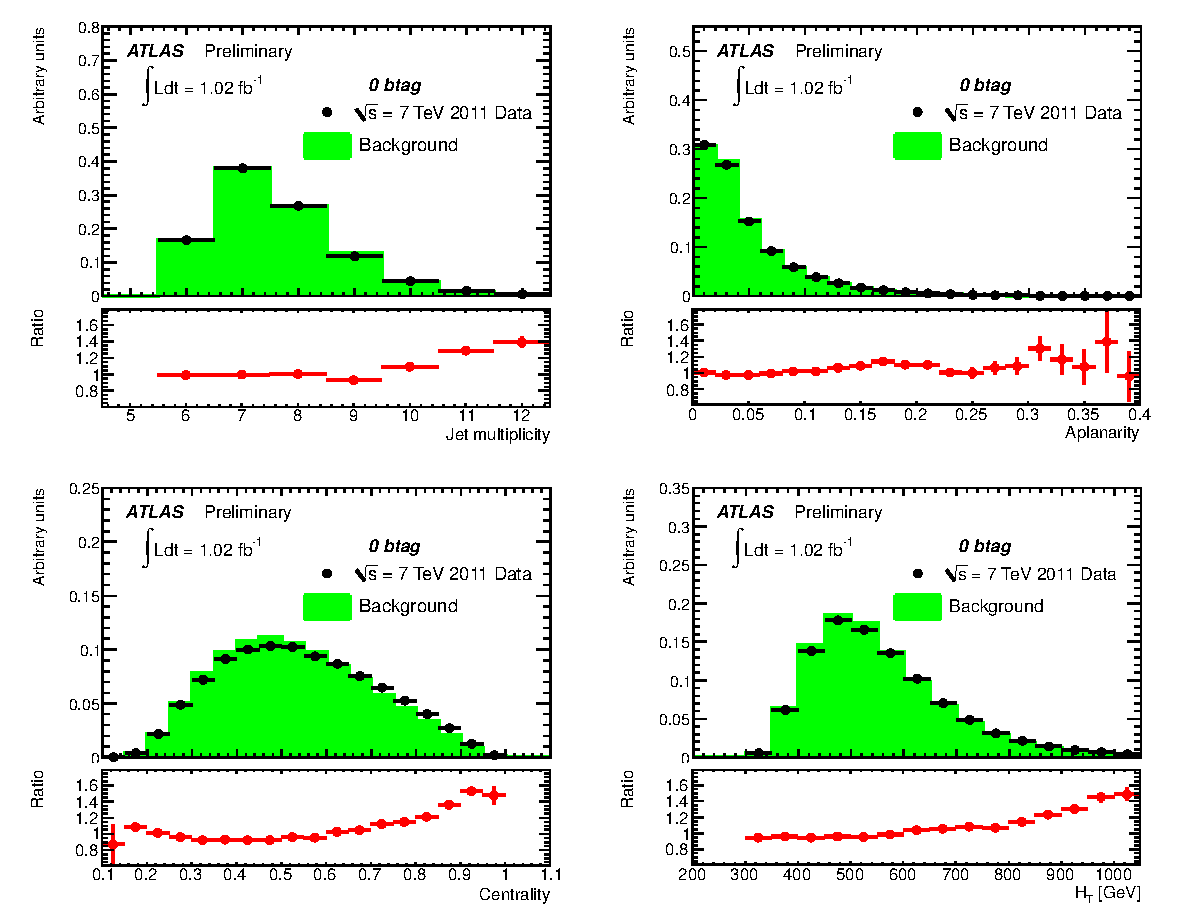
\includegraphics[width=0.95\linewidth]{figures/allhad/plot_control_5jets_0btag_ratio_24092011.eps} 
  \end{center}
  \caption{Comparison between inclusive six-jets data (dots) and the prediction modelled from five jet data for events without $b$-tagging for the number of jets, the aplanarity, the centrality and H$_T$. All histograms are normalized to have integral equal to one. Also shown the ratio between data and prediction.}
  \label{fig:control_5jets_0btag.eps}
\end{figure} 



\subsection{Systematic uncertainties and Cross-section measurement}
\label{sec:xsec}

To construct a likelihood function that separates signal from background,
a discriminating variable is constructed which resembles the $\chi^2$ of the kinematics
of an events under the signal hypothesis.
\begin{equation}
\chi^2 =  \frac{ \left(m_{j_1, j_2} - m_{W}\right)^2}{\sigma_W^2} + \frac{ \left(m_{j_1, j_2, b_1} - m_{t}\right)^2}{\sigma_t^2} + \frac{ \left(m_{j_3, j_4} - m_{W}\right)^2}{\sigma_W^2} + \frac{ \left(m_{j_3, j_4, b_2} - m_{t}\right)^2}{\sigma_t^2}, 
\end{equation}

Distributions for this variable are estimated for the $\ttbar$ signal using Monte Carlo simulation and for the QCD background using the EventMixing technique.
The scale and shapes of the templates for signal and background are succeptable to effects from a number of different sources.
These sources of systematic uncertainty, which are described below, effect the shapes and overall normalizations of the templates
representing the $\chi^2$ discriminating variable, and the effect of these uncertainties are incorporated into the likelihood
function using the modeling techniques of HistFactory.

%% Most of the systematic uncertainties are related to the signal modelling because the background is estimated by
%% a data-driven method. The only systematic uncertainty assigned to background is the background shape
%% modelling. For the signal $\ttbar$~MC sample, the systematic uncertainties are divided into shape and acceptance
%% effects. The relative shape and acceptance uncertainties are simultaneously taken into account.
%% The following systematic sources are considered together with an indication of whether they affect the shape or acceptance, or both:

The most important sources of systematic uncertainty in this analysis come from uncertainties on the Jet energy scale,
the efficiency of reconstructing jets based on the selection of this analysis, the resolution of reconstructed jets,
the efficiency of the multi-jet triggers, 
effects resulting from readout errors in the Liquid Argon calorimeter of ATLAS detector, 
and the energy scale of $b$-tagged jets.
In addition, a number of effects coming from the generation of the $\ttbar$ signal are considered, 
including differences seen across generators, effects of the level of parton shower considered, 
the parton distribution functions used,
and the rate of initial and final state radiation assumed.
Uncertainties on the measured amount of integrated luminosity are included, which effect the overall
normalization of the signal (but not the background, as it is derived from a data-driven technique).
Finally, the uncertainty on the background estimation is determined using a data-driven technique.
The uncertainty is estimated by comparing the shape of the QCD template in the signal region extracted
from either an exclusive 4-jet control region or an exclusive 5-jet control region separately.
The difference between these two extracted templates is taken as the size of the background uncertainty.


%% \item Background modelling [Event Mixing]:\\
%% The background-modelling systematic uncertainty is estimated using a four-jet event sample. 
%% The inclusive six-jet QCD background can be modelled with the two independent
%%   exclusive samples made respectively of four-jet events and five-jet events. The effect of the difference between the QCD inclusive six-jet sample built from the exclusive four-jet sample and the one produced from the exclusive five-jet one, is included as a systematic uncertainty in the $\ttbar$ production cross-section. This additional modelling uncertainty, illustrated in the right-hand panel of Figure \ref{fig:chi2.eps},  is applied to the analysis based on the five-jet trigger signature bin-by-bin to the $\chi^2$ template distribution obtained from the inclusive six-jet sample modelled from the exclusive five-jet sample. The change in the derived cross-section of 12.1\% is quoted as the associated systematic uncertainty.\\
%% An additional validation of the mixing method is performed trying it on the untagged five-jet data to predict the untagged six-jet data. The agreement on the $\chi^2$ is shown in the left-hand panel of Figure \ref{fig:chi2.eps}.\\
%% The dependency of the background modelling on the $|\Delta \pt|$ constraint between the two leading jets as well as for the fifth jets is checked. The $|\Delta\pt|$ constraint is varied from 1~GeV to 15~GeV and the maximal variation is found to be 2.3\%.



%% \begin{itemize}
%% \item Jet energy scale (JES) and associated uncertainty~\cite{ref:jessys}, [shape and acceptance]:\\
%% The jet energy scale and its uncertainty have been derived by combining information from test-beam data, LHC collision data and simulation. The residual differences between data and Monte Carlo simulation 
%% have been propagated through the analysis. Additional uncertainties due to the large pile-up effects in the 2011 data are included and range from 2\% to 7\% as a function of the jet $\pt$ and $|\eta|$.
%% The effect of JES systematics is estimated to be 24\%.

%% \item Jet reconstruction efficiency (JRE), [shape and acceptance]:\\
%% The difference in jet reconstruction efficiency between Monte Carlo simulation and data is propagated as a systematic uncertainty to Monte-Carlo. 
%% The effect of JRE uncertainty amounts to 0.1\%.

%% \item Jet energy resolution (JER)~\cite{ATLAS-CONF-2010-054}, [shape and acceptance]:\\
%% The simulated jets are smeared to match the jet energy resolution of the data. The uncertainty due to the resolution is estimated by varying the smearing factor according to the estimated uncertainties. The effect of JER is estimated to lead to an uncertainty of 13.5\%.

%% \item Trigger efficiency, [acceptance only]:\\
%% Events were selected with the five-jet trigger and by requiring the fifth-jet $\pt > 55$~GeV. The associated efficiency ranges from 
%% 90\% to 100\%, so a conservative 10\% systematic uncertainty is assigned to the trigger turn-on curve.

%% \item LAr readout problem, [acceptance only]: \\
%% A large fraction of the data (89.4\%) used in this analysis was collected in a period during which six out of 1524 front-end boards of the liquid Argon calorimeter could not be read out. As a consequence, in the data, events with an electron or a jet pointing in the direction of this inactive region were vetoed. The same procedure is applied to the simulated events. A corresponding systematic uncertainty is evaluated by varying the jet energy threshold by $\pm$4~GeV. The systematics on the cross-section amounts to 0.6\%.

%% \item $b$-tagging scale-factor (bSF) uncertainty, [shape and acceptance]:\\
%% To take into account possible differences in $b$-tagging efficiency between data and MC simulations, a set of scale factors parameterised as a function of jet $\pt$ and $\eta$ were applied to $b$-~,~$c$- and light-jets. These scale factors were varied individually within their maximal associated uncertainty and propagated through the analysis. The bSF systematic uncertainty leads to a 23\% uncertainty on the cross-section. This large uncertainty is due to the significant number of $c$-tagged jets, since the $c$-tagging uncertainty was conservatively assessed to be 20\% ( twice  the $b$-tag scale factor uncertainty). 
%% %This large uncertainty is due to the presence of $c$-tagged jets and the large uncertainty associated with the knowledge of 
%% %tagging them: twice

%% \item Generator and parton shower (PS) dependency [shape and acceptance]:\\
%% The uncertainty due to the modelling of the $\ttbar$ signal is quantified by replacing the  {\sc MC@NLO} Monte Carlo generator with {\sc POWHEG} and {\sc PYTHIA}~\cite{SJO-0601} for modelling the $\ttbar$ signal sample. The systematic uncertainty is estimated to be 5.4\%.

%% \item Initial and Final State Radiation (ISR and FSR), [shape and acceptance]:\\
%% The effects of variations in the amount of initial and final state radiation (ISR/FSR) were studied
%% using the {\sc AcerMC}~\cite{KER-0401} generator interfaced to {\sc PYTHIA} by varying the parameters controlling
%% ISR and FSR in a range consistent with experimental data. The systematic uncertainty is taken as half the maximum difference between any two samples. It amounts to 23\%.
%% %% The effects of variations in the amount of initial and final state radiation (ISR/FSR) were studied
%% %% using the AcerMC generator interfaced to PYTHIA  by varying the parameters controlling
%% %% ISR and FSR in a range consistent with experimental data. The maximum difference
%% %% between pairs of samples with reduced and increased ISR and FSR is taked as the final systematics. It amounts to 23.4\%.

%% \item Parton Distribution Function (PDF), [acceptance only]:\\
%% The uncertainty associated to the PDF is evaluated with CTEQ6.6 and its error sets. For each of the error settings, the final cross-section
%% is derived and the final uncertainty is calculated. The effect of PDF uncertainty amounts to 8.6\%.

%% \item Luminosity [acceptance]:\\
%% The uncertainty on the luminosity propagates linearly to the cross-section measurement, leading to a systematic uncertainty of $3.7\%$~\cite{ref:lum}. 

%% \item Background modelling [Event Mixing]:\\
%% The background-modelling systematic uncertainty is estimated using a four-jet event sample. 
%% The inclusive six-jet QCD background can be modelled with the two independent
%%   exclusive samples made respectively of four-jet events and five-jet events. The effect of the difference between the QCD inclusive six-jet sample built from the exclusive four-jet sample and the one produced from the exclusive five-jet one, is included as a systematic uncertainty in the $\ttbar$ production cross-section. This additional modelling uncertainty, illustrated in the right-hand panel of Figure \ref{fig:chi2.eps},  is applied to the analysis based on the five-jet trigger signature bin-by-bin to the $\chi^2$ template distribution obtained from the inclusive six-jet sample modelled from the exclusive five-jet sample. The change in the derived cross-section of 12.1\% is quoted as the associated systematic uncertainty.\\
%% An additional validation of the mixing method is performed trying it on the untagged five-jet data to predict the untagged six-jet data. The agreement on the $\chi^2$ is shown in the left-hand panel of Figure \ref{fig:chi2.eps}.\\
%% The dependency of the background modelling on the $|\Delta \pt|$ constraint between the two leading jets as well as for the fifth jets is checked. The $|\Delta\pt|$ constraint is varied from 1~GeV to 15~GeV and the maximal variation is found to be 2.3\%.

%% \item Background modelling [ABCD]:\\
%% The estimate of the \mj contamination derived with the ABCD
%% technique relies on the hypothesis that the centrality and
%% $\vartheta$ are uncorrelated. A specific uncertainty is then associated to this measurement.
%% Firstly, a correlation of $2\%$ between centrality and $\vartheta$ is
%% estimated from QCD \mj Monte Carlo samples. 
%% Such a correlation results in a relative uncertainty of 
%% $15\%$ on the cross-section obtained with the ABCD method.
%% Secondly, the centrality shape of background events was
%% reproduced with the Event Mixing technique using four-jet and five-jet events. The shape derived from the data with this method was compared between the \Br~\Dr~ and \Ar~\Cr~ regions.
%% The shapes are verified to agree to within about 1\%.
%% The value of  $\frac{{\rm N_{QCD}}^{C}}{{\rm N_{QCD}}^{A}}\times\frac{{\rm
%%  N_{QCD}}^{B}}{{\rm N_{QCD}}^{D}}$ is evaluated and found to be $1.05$.
%% This factor was introduced in Equation~\ref{eq:abcd-qcd} and gives a $30\%$
%% systematic effect on the cross-section. This value was taken as
%% the systematic uncertainty due to the correlation between the centrality and $\vartheta$.\\
%% \end{itemize}

The difference between the extracted templates using these two control regions is showin in figure ~\ref{fig:chi2.eps}
\begin{figure}[h!]
  \begin{center}
%    \includegraphics[width=0.35\linewidth]{figures/chi2.eps} 
    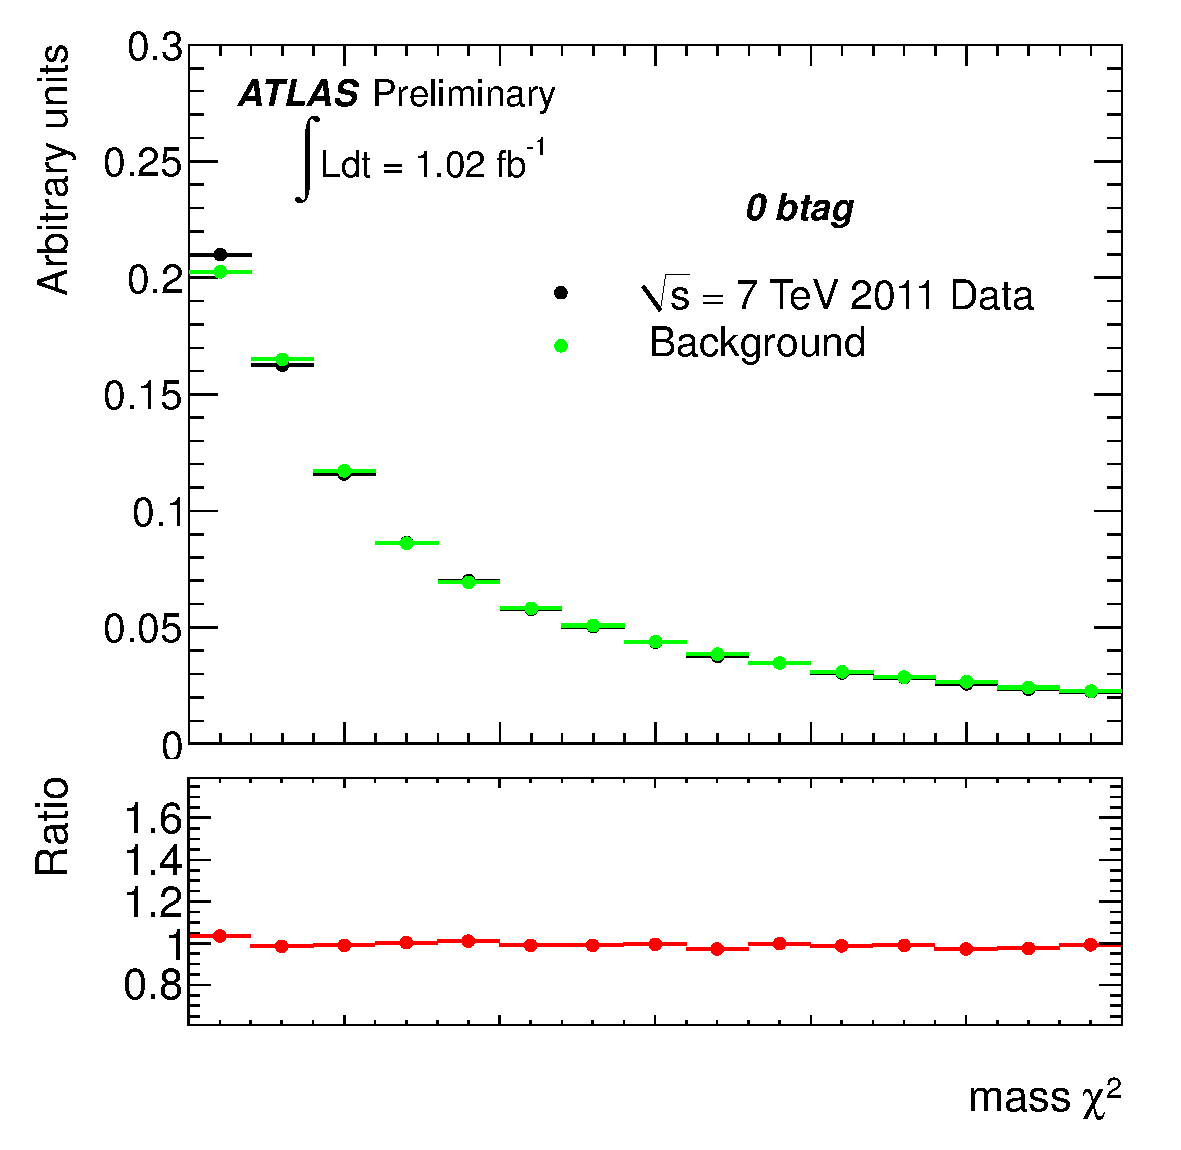
\includegraphics[width=0.45\linewidth]{figures/allhad/plot_chi2_0btag_21092011.eps} 
    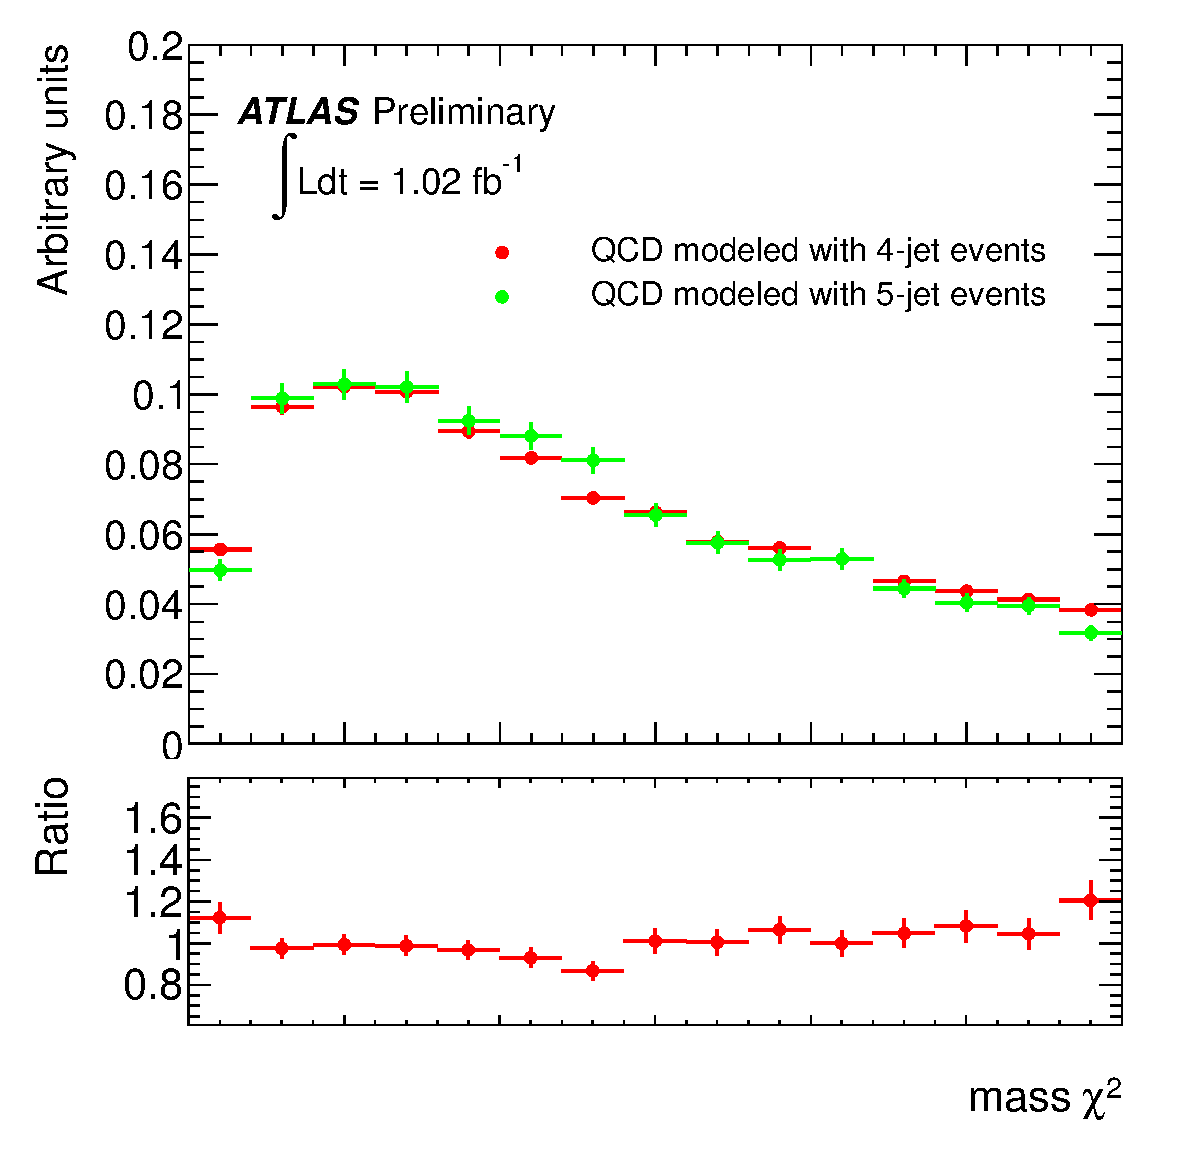
\includegraphics[width=0.45\linewidth]{figures/allhad/plot_bkgchi2_21092011.eps}\\
  \end{center}
  \caption{Left: $\chi^2$ comparison between inclusive six-jets data (dots) and the background modelled from five-jet data (green) for events without $b$-tagging. Right: comparison of the two $\chi^2$ distributions for the inclusive six-jet modelled with four-jet data (red) and the inclusive six-jet modelled with five-jet data for the four-jet trigger selected events, all events have at least two $b$-tagged jets. All histograms are normalized to have integral equal to one.}
  \label{fig:chi2.eps}
\end{figure} 

The size of the effects from systematic uncertainties are summarized in Table \ref{tab:finaluncertainties}.

    \begin{table}[!h]
    \begin{center}
      \begin{tabular}{c|c}
          \hline
              \hline
              Source of uncertainty            &  Size of the effect (\%)\\
              \hline
              Jet energy scale              &          24.2    \\
              Jet reconstruction efficiency &           0.1    \\
              Jet energy resolution         &          13.5    \\
              Multi-jet trigger             &          10.0    \\
              LAr readout problem           &           0.6    \\
              $b$-tagging                   &          23.0    \\
              Generator (PS., Hadronisation)&           5.4    \\
              ISR, FSR                      &          23.4    \\
              PDF                           &           8.6    \\
              Luminosity                    &           3.7    \\
              Multi-jet modelling           &          12.1    \\
              \hline
              \hline
              Total                         &          46.7    \\
              \hline
              \hline

              \end{tabular}
              \end{center}
               \caption{Summary of the different systematic uncertainties associated with the $\chi^2$
                template fit of the selected data events to the $\ttbar$ signal and \mj
                 QCD mixed sample. Uncertainties are given in \%. For the systematic uncertainties associated with the PDF, in the case of the ABCD method, the maximal variation derived from the Event Mixing based analysis is used.}
                   \label{tab:finaluncertainties}
                   \end{table}

Finally, a likelihood function is constructed that models the total distribution of the $\chi^2$ discriminant in data
as a combination of $\ttbar$ signal and QCD background.
\begin{equation}
L(f_s) = \Pi_{i} \frac{ \mu^{n_{i}} \exp(-\mu_i) }{n_{i}!}; \ \  \mu_{i} = N_{{\rm data}} \times ( f_s \times P_{i,t\bar{t}}  + (1 - f_{s}) \times P_{i,{\rm QCD}}).
\end{equation}
where $P_{t\bar{t}}$ and $P_{{\rm QCD}}$ are the fraction of $\ttbar$ and QCD events falling into the ith bin of the discriminating variable, 
$f_s$ is a parameter representing the fraction of events coming from $\ttbar$ signal, 
and $N_{{\rm data}}$ is the total number of observed events.
The $\ttbar$ cross-section is excracted by fitting this likelihood function to data while allowing the relative amount of signal to float.
The result of the likelihood fit is shown in Figure \ref{fig:fitchi2_3_Jet.eps}. 
The measured value of the top-quark pair-production cross-section is measured to be:
\begin{equation*}
 \sigma {(pp \to t\bar{t})} = 167 \pm 18 \; {\rm (stat.)} \; \pm 78 \; {\rm (syst.)} \;  \pm 6 \;  {\rm (lum.)} \; {\rm pb}
\end{equation*}
which is compatible with the Standard Model expectation of  $\sigma_{{\rm SM}} = 164^{+11} _{-16}$~pb.


%The signal content is estimated to be $f_{s}~=~$~( 24.0 $\pm$ 2.4)\% and the total $\ttbar$~cross-section $\sigma = 167 \pm 18$ (stat.) pb.

\begin{figure}[h!]
  \begin{center}
    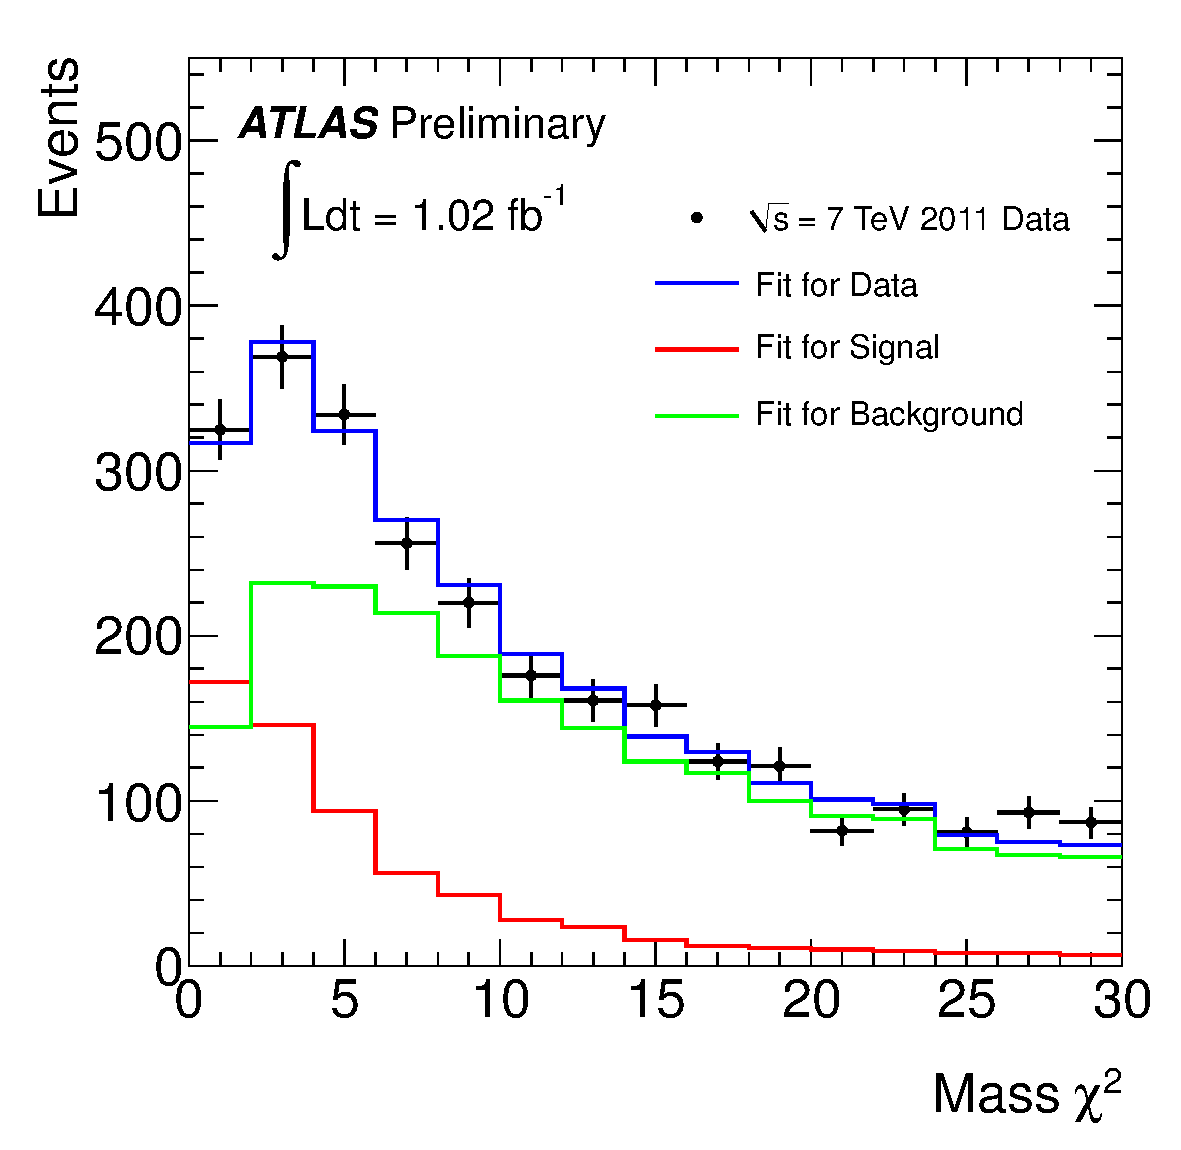
\includegraphics[width=0.75\linewidth]{figures/allhad/plot_fitchi2_21092011.eps}
  \end{center}
  \caption{Fit of the minimal mass $\chi^2$ distribution with the binned likelihood (blue line) to the selected data (dots). The $\ttbar$~signal fitted fraction is shown in red and the QCD inclusive six-jet background  in green. The errors bars associated to the data are statistical only.}
  \label{fig:fitchi2_3_Jet.eps}
\end{figure}

%% \subsection{Cross-section measurement}
%% \label{sec:xsec}

%% \noindent To test the compatibility of selected events with the $\ttbar$ hypothesis by assigning jets to the different decay products and looking at the consistency of the kinematics with the expected top quark and $W$ boson masses, a $\chi^2$-based discriminant observable was implemented. It aims to extract the $t\bar{t}$ signal from the \mj background. 

%% If there are more than two  $b$-tagged jets, the $\chi^2$ minimization chooses the two 
%% $b$-jets and the remaining $b$-tagged jets will not be used to reconstruct the $\ttbar$ system.
%% The same principle applies in the case of more than six jets where again the $\chi^2$ minimization chooses which six jets 
%% (including the two $b$-jets) will be used to form the candidate $\ttbar$ pairs.
%% The $\chi^2$ is built for each one of the six $t\bar{t}$ hypothesis. For a given event, the correct jet assignment is identified as the jet combination which minimises
%% \begin{equation}
%% \chi^2 =  \frac{ \left(m_{j_1, j_2} - m_{W}\right)^2}{\sigma_W^2} + \frac{ \left(m_{j_1, j_2, b_1} - m_{t}\right)^2}{\sigma_t^2} + \frac{ \left(m_{j_3, j_4} - m_{W}\right)^2}{\sigma_W^2} + \frac{ \left(m_{j_3, j_4, b_2} - m_{t}\right)^2}{\sigma_t^2}, 
%% \end{equation}
%% \noindent and is used to select, among the different jets, which jets to assign to each $W$ boson and top quark.
%% \noindent The $\ttbar$ signal and the background mass $\chi^2$ templates modelled respectively with MC@NLO and the Event Mixing technique described in the previous sections, are fitted to the $\chi^2$ output for the selected data events. 
%% The $\ttbar$ signal fraction and thereby the background normalization are extracted from the likelihood fit of the $\chi^2$ distribution. The likelihood is defined as:
%% \begin{equation}
%% L(f_s) = \Pi_{i} \frac{ \mu^{n_{i}} \exp(-\mu_i) }{n_{i}!}; \ \  \mu_{i} = N_{{\rm data}} \times ( f_s \times P_{i,t\bar{t}}  + (1 - f_{s}) \times P_{i,{\rm QCD}}).
%% \end{equation}
%% where $f_s$ is a parameter corresponding to the signal fraction in data and $N_{{\rm data}}$ is the number of observed data events. The symbols $P_{t\bar{t}}$ and $P_{{\rm QCD}}$ are the probabilities in the $i$-th $\chi^2$ bin extracted from the $\ttbar$ signal and QCD \mj modelled background templates. The derived number of $\ttbar$ events is then used to estimate the $\ttbar$ cross-section defined as $ \sigma_{\ttbar} = f_{s} N_{{\rm data}} / L\epsilon$, where $L$ is  the integrated luminosity and $\epsilon$, the signal selection efficiency in 
%% an inclusive $\ttbar$ sample, which includes the non all-hadronic decay modes, is estimated to be $(0.380 \pm 0.015)\%$  using the MC@NLO generator. The result of the likelihood fit is shown in Figure \ref{fig:fitchi2_3_Jet.eps}. The signal content is estimated to be $f_{s}~=~$~( 24.0 $\pm$ 2.4)\% and the total $\ttbar$~cross-section $\sigma = 167 \pm 18$ (stat.) pb.

%% Figure \ref{fig:fitchi2_4_Jet.eps} shows the top mass distribution for the selected candidates, using the jet combinations that minimize a mass $\chi^2$ in which the two $(m_{j, j, b} - m_{t})$ terms are substituted by $(m_{j_1, j_2, b_1} - m_{j_3, j_4, b_2})$, i.e. the difference between the mass of the two three-jet triplets. 
%% This $\chi^2$  does not make use of the top mass constraint, but only constrains the masses of the two triplets to be equal,
%%  allowing the mass that minimizes the term to be away from $m_{t}$.
%% For the plot shown in Figure \ref{fig:fitchi2_4_Jet.eps} the signal and background are normalized to the cross-section measured using the $m_{t}$ constraint.   


%% \begin{figure}[h!]
%%   \begin{center}
%% %    \includegraphics[width=0.8\linewidth]{figures/fitchi2_3_Jet.eps} 
%% %    \includegraphics[width=0.8\linewidth]{figures/plot_chi2Fit_07092011.eps} 
%%     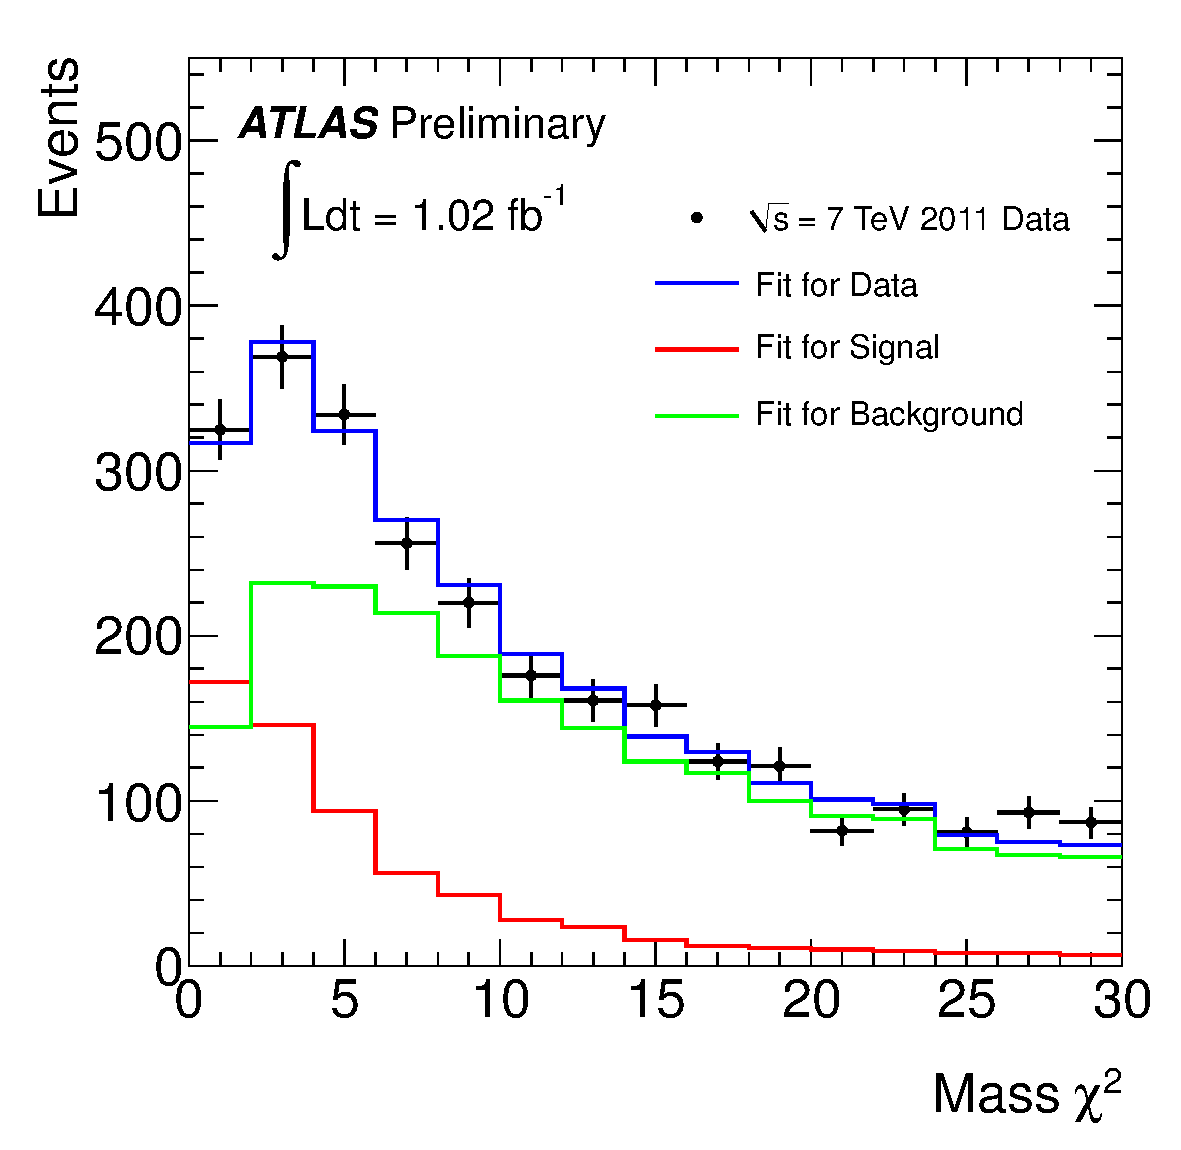
\includegraphics[width=0.75\linewidth]{figures/allhad/plot_fitchi2_21092011.eps} 
%%   \end{center}
%%   \caption{Fit of the minimal mass $\chi^2$ distribution with the binned likelihood (blue line) to the selected data (dots). The $\ttbar$~signal fitted fraction is shown in red and the QCD inclusive six-jet background  in green. The errors bars associated to the data are statistical only.}
%%   \label{fig:fitchi2_3_Jet.eps}
%% \end{figure} 

%% \begin{figure}[h!]
%%   \begin{center}
%% %    \includegraphics[width=0.8\linewidth]{figures/fitchi2_3_Jet.eps}
%% %    \includegraphics[width=0.8\linewidth]{figures/plot_chi2Fit_07092011.eps}
%%     \includegraphics[width=0.75\linewidth]{figures/allhad/plot_tripletMass_172GeV.eps}
%%   \end{center}
%%   \caption{Top mass reconstructed from minimal mass $\chi^2$ distribution without top-quark mass constraint, signal and background are normalized according to the result of the fit shown in Figure \ref{fig:fitchi2_3_Jet.eps}. The errors bars represent the statistical uncertainties while the hatching represent the systematic ones. }
%%   \label{fig:fitchi2_4_Jet.eps}
%% \end{figure}



%% \subsubsection{A cross check of the Event Mixing background estimation: kinematical fit of the top mass. }
%% \label{sec:klf}

%% After performing the cross section extraction we can use a kinematic fit of the top mass as a cross check 
%% for the validity of the background modeling carried out using the Event Mixing technique. 
%% KLFitter, previously used in top analyses in the lepton plus jets channel~\cite{ATLAS-CONF-2011-033,ATLAS-CONF-2011-037}, 
%%  make use of a likelihood approach to analyze the decay of the $\ttbar$ system.  
%% Using event kinematics and the known decay chain of the top and anti-top, one is able to reconstruct the proper decay 
%% particles. The basic likelihood, which is comprised of only kinematic elements, is
%% \begin{eqnarray}
%% \rm{L_{kin}} & = &
%% \rm{BW}\left\{m(q_1 q_2) \; | \; m_W, \Gamma_W\right\} \cdot
%% \rm{BW}\left\{m(q_3 q_4) \; | \; m_W, \Gamma_W\right\} \cdot \nonumber \\
%% &&
%% \rm{BW}\left\{ m(q_1 q_2 b_1) \; | \; m_{\mathrm{top}}, \Gamma_{\mathrm{top}} \right\} \cdot
%% \rm{BW}\left\{ m(q_2 q_3 b_2) \; | \; m_{\mathrm{top}}, \Gamma_{\mathrm{top}}\right\} \cdot \nonumber \\
%% &&
%% \rm{W}\left(\tilde{E}_{\mathrm{jet}_1} \; | \; E_{b_1} \right) \cdot
%% \rm{W}\left(\tilde{E}_{\mathrm{jet}_2} \; | \; E_{b_2} \right) \cdot
%% \rm{W}\left(\tilde{E}_{\mathrm{jet}_3} \; | \; E_{q_1} \right) \cdot
%% \rm{W}\left(\tilde{E}_{\mathrm{jet}_4} \; | \; E_{q_2} \right) \cdot \nonumber \\
%% &&
%% \rm{W}\left(\tilde{E}_{\mathrm{jet}_5} \; | \; E_{q_3} \right) \cdot
%% \rm{W}\left(\tilde{E}_{\mathrm{jet}_6} \; | \; E_{q_4} \right).
%% \end{eqnarray}

%% \noindent The elements of the likelihood include Breit-Wigner components (BW) and transfer functions (W) for different p$_{T}$ 
%% and $\eta$ regions.  The likelihood describes the decay of a $\ttbar$ system.  The four Breit-Wigner fits describe 
%% the original top and anti-top quark decays into a $b$ and $W$ and the subsequent $W$ boson decays into two quarks.  
%% The transfer functions are derived from MC@NLO Monte Carlo.  To further improve the reconstruction efficiency we also include $b$-tagging information in the likelihood. 

%% For all events passing the preselection and having at least six jets within $| \eta | <$~2.5 we apply KLFitter algorithm, as well to 
%% background events modeled with the Event Mixing and Monte Carlo $\ttbar$ signal.
%% As shown in Figure~\ref{fig:klf_mass} the kinematical fit of the top mass confirms that the presence of top quark can be 
%% observed indipendently as an excess over the QCD \mj background which is consistent with the $\ttbar$ hypothesis.

%% \begin{figure}[h!]
%%   \begin{center}
%% %      \includegraphics[width=0.6\linewidth]{figures/klf_mass.eps} 
%%       \includegraphics[width=0.6\linewidth]{figures/allhad/klf_mass_07092011.eps} 
%%       \caption{Results of the KLFitter on events passing the preselection having at least six jets within $| \eta | <$~2.5. The $t\bar{t}$ signal is normalized to the cross section measured with the likelihood fit of the $\chi^2$ distribution while the background shape is 
%%       estimated with the Event Mixing method.} 
%%   \label{fig:klf_mass}
%%   \end{center}
%% \end{figure} 



%% \subsection{ABCD analysis}

%% A second technique is used relying on a simple ABCD method, counting events in control
%% region and a signal region. The background in the signal region is extracted
%% from the yield in the control regions.

%% %These data driven approaches reduce the impact of the simulation driven systematic effects
%% %like the Monte Carlo sample size, the \mj background cross-sections and modeling.

%% \subsubsection{Background estimation}

%% %\noindent The aim of this method is to extract the observed number of \mj \ttbar
%% %events. This measurement relies on the \mj background estimation both in terms
%% %of number of events and in terms of observable shape.

%% %\noindent The ABCD method relies on the shape conservation of a selection observable when another set of uncorrelated variables is used
%% % to select the events. The following couple of variables which are assumed to be uncorrelated is used~:
%% %\begin{itemize}
%% %   \item The event centrality ;
%% %   \item The presence of at least two b-tagged jets verifying ${\Delta}R_{b\bar{b}}$.
%% %\end{itemize}

%% \noindent  Two variables are used to characterize the signal: the centrality
%%  of the event and $\vartheta$ which is defined as follows~:
%% \begin{itemize}
%%   \item $\vartheta=1$ if the event contains at least two b-tagged jets
%%   verifying $\Delta R > 1.2$
%%   \item $\vartheta=0$ if the event does not verify the first condition but
%%   contains one b-tagged jet.
%% \end{itemize}
%% Events with no b-tagged jet are rejected. These two variables have been chosen such
%%  they are uncorrelated.

%% % The overall acceptance, $\epsilon_s$ for the signal is estimated to be about
%% % $2\%$ using the Monte Carlo simulation.
%% % The acceptance of the trigger and the b-tagging cuts are corrected
%% % according to dedicated studies~[ ].
%% % A scale factor, $k$, will describe the product of
%% % the acceptance corrections and is applied to $\epsilon_s$.



%% %\begin{table}[htbp]
%% %  \small
%% %  \centering
%% %  \begin{tabular}[]{c c  c c c c c }
%% %
%% %     Cut & Signal & \btt & \wj  &  \zj & \st &   \\    \hline 
%% %     at least 2 distant b-jets & $ $ & $ $ & $ $  &  $ $ & $ $   \\
%% %     
%% %     Centrality $> 0.6$ & $ $ & $ $ & $ $  & $ $ & $ $   \\    \hline 
%% %
%% %
%% %  \end{tabular}
%% % \caption{\small Expected number of events and selection acceptance for a
%% % luminosity of $~pb^{-1}$. The signal number of events are given assuming a
%% % production cross section of $75~pb$.}
%% % \label{tab:sel_stat} 
%% %\end{table}

%% %The correlation between these two variables is evaluated on a Monte Carlo
%% %simulation of multi-jet events and found to be about $2\%$.

%% Four independent regions are defined: a
%% signal enriched region, so called \Dr region, and three control  regions, quoted \Ar,
%% \Br and \Cr dominated by
%%  \mj background events. They are defined in table~\ref{tab:abcd_regions}
%% where the expected and the observed number of events are
%% given. Figure~\ref{fig:2d_signal_data} shows the distribution of the events in
%% the plane defined by the two variables.


%% \begin{table}[htbp]
%%   \small
%%   \centering
%%   \begin{tabular}[]{c c  c c c c c c }

%%      Sample & first variable & second variable  & $\epsilon_{i}^{tt}[\%] $ & Signal~[events] & $n_i$~[events] &  $\rho$~[\%] & ${\rm N}_i$~[events] \\    \hline 
%%      D & $\vartheta = 1$ & Centrality $> 0.65$ & $0.34$ & $501.3$ & $13.0$ & $23.5\%$ & $2466$ \\
%%      B & $\vartheta = 1$ & Centrality$ < 0.65$ & $0.36$ & $498.5$ & $16.7$  & $10.1\%$ & $6112$ \\    
%%      C & $\vartheta = 0$ & Centrality $> 0.65$ & $0.49$ & $720.7$ & $42.8$ & $7.06\%$ & $11880$ \\
%%      A & $\vartheta = 0$ & Centrality $< 0.65$ & $0.57$ & $775.5$ &  $50.3$ & $2.9\%$ & $33036$ \\ \hline


%%   \end{tabular}
%%  \caption{\small Definition of the four regions, A, B, C and D. $n_i (i=a,b,c,d)$ are the contributions of W+jet,
%%  Z+jet, single top and di-boson final states. The purities and the
%%  efficiencies, $\rho$ and $\epsilon^{t\bar{t}}$, are given for all \ttbar events,
%%  including the semileptonic decays. ${\rm N}_i$ are the observed number of events in each sample.}
%%  \label{tab:abcd_regions} 
%% \end{table}


%% \begin{figure}[h!]
%%   \begin{center}
%%     \begin{tabular}{cc}
%%       \includegraphics[width=0.4\linewidth]{figures/allhad/signal_box_abcd.eps}
%%       &  \includegraphics[width=0.4\linewidth]{figures/allhad/data_box_abcd.eps} \\
%%     \end{tabular}
%%   \end{center}
%%   \caption{Distribution of simulated signal events (left) and of data events
%%   (right) in the plane defined by the centrality and a logical variable
%%   describing the presence of at least 2 b-tagged and distant b-jets.}
%%     \label{fig:2d_signal_data}
%% \end{figure} 



%% The numbers of \mj background events in these four samples verify~:
%% $${\rm N_{QCD}^{d}} \simeq \frac{{\rm N_{QCD}}^{c}}{{\rm N_{QCD}}^{a}} {\rm
%%   N_{QCD}}^{b}$$

%% The contribution of the W+jet, Z+jet, single top and di-boson final states are
%% quoted \ba, \bb, \bc and \bd. They are estimated using the Monte Carlo simulations and
%% given in Table~\ref{tab:abcd_regions}.

%% The total number of events observed in the control samples are quoted \Na,
%% \Nb and \Nc. Assuming typical cross sections of $164~pb$ for the signal, the
%% signal fraction within in the three control
%% samples vary from $3$ to $8\%$. These signal events will then have to be taken into
%% account. 

%% The number of \mj background events in the
%% selected sample can then be written as:

%% $$ {\rm N}_{\rm QCD}(\sigma) = \left({\rm N}_{d} - n_{d} -
%%     \epsilon_{d}^{t\bar{t}}\sigma L\right) = \frac{\left({\rm
%%     N}_{b}- n_{b}-\epsilon_{b}^{t\bar{t}}\sigma L\right) \left({\rm
%%     N}_{c}- n_{c}-\epsilon_{c}^{t\bar{t}}\sigma L\right)  }{ \left({\rm
%%     N}_{a}- n_{a}-\epsilon_{a}^{t\bar{t}}\sigma L\right) } $$

%% where the acceptances $\epsilon_i^{t\bar{t}}$ ($i=a,b,c,d$) are extracted from the
%% simulation. They are defined using all the \ttbar~ decays after the multi-jet
%% selection. This second order equation involving the observed number of events and the signal
%% efficiencies only can be solved:

%% \[
%%  {\rm N}_{\rm QCD}(\sigma) = N_{d} - n_{d} - L\epsilon_{d}^{t\bar{t}} \left(
%%  \frac{-b \pm \sqrt{\Delta}}{2a} \right)
%%  \label{eq:abcd-qcd}
%% \]

%% where
%% $
%% a = L^2 \left( \epsilon_d^{t\bar{t}} \epsilon_a^{t\bar{t}} - \epsilon_b^{t\bar{t}} \epsilon_c^{t\bar{t}}  \right)
%% $, 
%% $
%% b = L \left( \epsilon_b^{t\bar{t}} (N_{c}-n_{c}) + \epsilon_c^{t\bar{t}} (N_{b}-n_{b}) - \epsilon_d^{t\bar{t}} (N_{a}-n_{a}) -
%% \epsilon_a^{t\bar{t}} (N_{d}-n_{d}) \right)
%% $, 
%% $
%% c = (N_{d}-n_{d}) (N_{a}-n_{a}) - (N_{b}-n_{b}) (N_{c}-n_{c})
%% $ and
%% $
%% \Delta = b^2 - 4ac
%% $.

%% Using the number of events shown on table~\ref{tab:abcd_regions} two solutions
%% are obtained, only one of them is positive.
%% % and equal $11212 \pm 295$
%% %events. This uncertainty is statistical only.

%% \subsubsection{Signal extraction and cross section measurement}

%% Using the formulae~\ref{eq:abcd-qcd} one can deduce the signal cross-section: 

%% \[ \sigma = -\frac{b}{2a} \pm \frac{\Delta}{2a} \]

%% The statistical uncertainty on $\sigma$ is evaluated by propagating the
%% uncertainties on $N_a$, $N_b$, $N_c$ and $N_d$ to the measurement. This
%% uncertainty includes the statistical precision on the \mj background. 
%% Using the number of events given in Table~\ref{tab:abcd_regions}, the signal
%% cross-section is estimated to be $\sigma = 161.1 \pm 37.6~pb$.
%% % ($\sigma = 244,45 \pm 67,5 pb$ using the SV1 b-tagger).

%% \subsubsection{Uncertainties due to the ABCD method}

%% The estimation of the \mj contamination derived with the ABCD
%% technique relies on the uncorrelation hypothesis between the centrality and
%% $\vartheta$. In addition to the systematic effects described with the previous
%% method a specific uncertainty is associated to this measurement.
%% In one hand, a correlation of $2\%$ between the centrality and $\vartheta$ is estimated on
%%   the Monte Carlo simulation of \mj background events using Alpgen bb+nparton samples. Such a correlation
%%   propagates to the ratio $\frac{{\rm N_{QCD}}^{c}}{{\rm N_{QCD}}^{a}} {\rm 
%%   N_{QCD}}^{b}$ by an effect of $3.5\%$. 

%% In the other hand, the centrality shape of background events was
%% reproduced with the {\it Event mixing} 
%% technique using four and five jet events. The shape derived from the data with this method was compared between \Br\Dr and \Ar\Cr regions as shown on
%% Figures~\ref{fig:abcd-syste-cent-mixing}. The agreement is verified at the level of $1\%$.
%% The value of  $\frac{{\rm N_{QCD}}^{c}}{{\rm N_{QCD}}^{a}}\times\frac{{\rm
%%  N_{QCD}}^{b}}{{\rm N_{QCD}}^{d}}$ is evaluated and found to be different from 1 by $5\%$.
%% % This value is the systematic uncertainty on the subtracted \mj background.
%% This factor of $1.05$ was introduced in the equation~\ref{eq:abcd-qcd} leading to a systematic effect of $30\%$ on the cross-section.\\

%% \begin{figure}[h!]
%%   \begin{center}
%%     \begin{tabular}{cc}
%%       \includegraphics[width=0.4\linewidth]{figures/allhad/plot_centrality_ab_cd.eps}
%%       &  \includegraphics[width=0.4\linewidth]{figures/allhad/event_fraction_bd_ac.eps} \\
%%     \end{tabular}
%%   \end{center}
%%   \caption{Comparison between the centrality in the four regions
%%     using the Event mixing technique.}
%%     \label{fig:abcd-syste-cent-mixing}
%% \end{figure} 

%% \subsubsection{ABCD method}
%% The investigated effects in the case of the ABCD method, propagate to the cross section measurements through~:
%% \begin{itemize}
%%    \item Event selection acceptance;
%%    \item Background events estimate.
%% \end{itemize}

%% The estimation of the \mj contamination derived with the ABCD
%% technique relies on the uncorrelation hypothesis between the centrality et the
%% flavor content of the event. The centrality shape of background events is
%% reproduced with the {\it Event mixing} 
%% technique an can be compared between \Br\Dr and \Ar\Cr regions as
%% shown on Figure~\ref{fig:abcd-syste-cent-mixing}. The differences are
%% compatible with the correlation of $2\%$ estimated on the Monte Carlo
%% simulation of \mj events. Such a correlation propagates to the ratio $\frac{{\rm N_{QCD}}^{c}}{{\rm N_{QCD}}^{a}} {\rm
%%   N_{QCD}}^{b}$ and then to the measured cross section. Using the data-driven centrality
%% distributions, a difference in the centrality shape between the \Br\Dr and
%% \Ar\Cr regions can be quantified using the Figure~\ref{fig:abcd-syste-cent-mixing}(right).
%%  This leads to a systematic effect of $5\%$ on the subtracted \mj background and then to a
%%  systematic effect of $35\%$ on the cross-section.

%% The largest remaining uncertainties associated to the method and derived using
%% dedicated simulations as described in the previous section. They
%% arise from the jet energy scale including pileup effects
%% ($\pm_{1.8}^{1.7}\%$),  the dead LAr regions 
%% ($\pm_{1.8}^{2.4}\%$), the jet energy resolution ($\pm 1.7\%$),
%% the jet reconstruction efficiency ($\pm 0.17\%$). The impact of
%% the the modeling of initial and final state radiation systematics was derived
%% by considering different settings of the generator parameters and yields to an
%% additional systematic uncertainty of $\pm 20\%$.

%% The uncertainty on the luminosity propagates linearly to the cross-section
%% measurement leading to a systematic uncertainty of $4.5\%$. 

%% \begin{figure}[h!]
%%   \begin{center}
%%     \begin{tabular}{cc}
%%       \includegraphics[width=0.4\linewidth]{figures/plot_centrality_ab_cd.eps}
%%       &  \includegraphics[width=0.4\linewidth]{figures/event_fraction_bd_ac.eps} \\
%%     \end{tabular}
%%   \end{center}
%%   \caption{Comparison between the centrality in the four regions
%%   using the Event mixing technique.}
%%     \label{fig:abcd-syste-cent-mixing}
%% \end{figure} 

%The different contributions to the total uncertainty are reported in table \ref{tab:finaluncertainties}.
%\begin{table}
%\begin{center}
%  \begin{tabular}{c||c|c||c|c}
%    \hline
%systematics source            &  \multicolumn{2}{c||}{\mj Event mixing} & \multicolumn{2}{c}{\mj ABCD} \\
%                              & {\tt JetComb}    &{\tt SV1}& {\tt JetComb} & {\tt SV1} \\
%Jet energy scale              &          24.2    & 22.2    &  18.9 & 16.4 \\
%Jet energy Resolution         &          13.5    & 13.5    &   7.3 & 2.5 \\
%Jet reconstruction efficiency &           0.1    &  0.1    &   0.3 & 3.5 \\
%Multijet trigger              &          10.0    & 10.0    &  10.0 & 10.0 \\   
%Dead LAr region               &           0.6    &  0.6    &   0.3  & 0.4 \\ 
%b-tagging                     &          23.0    & 21.9    &  30.0 & 31.0 \\ 
%ISR, FSR                      &          23,4    & 23.4    &  10.0 & 10.2 \\
%Generator                     &           5.4    & 4.6     &  15.0 & 7.0 \\    
%PDF                           &           8.6    & 8.9     &   8.9$^\star$& 8.9$^\star$ \\
%Luminosity                    &           3.7    & 3.7     &   3.5  & 3.5 \\   
%\hline
%\mj Modeling                  &           8.1    &10.4     & 30.0 & 30.0 \\
%\hline
%\hline
%Total                         &          45.9    &44.8     &   51.3 &  49.1 \\
%\hline
%\hline
%
%
%\end{tabular}
%\end{center}
% \caption{Summary of the different systematics associated to the chisquare
% template fit of the selected data events to the $\ttbar$ signal and multijet
% QCD mixed sample. Uncertainties are given in \% and evaluated for each one of
% the two tested b-taggers. For the systematics associated to the PDF, in the case of the ABCD method, the maximal variation derived from the Event-mixing based analysis is used.}
%  \label{tab:finaluncertainties}
%\end{table}

%% \begin{table}
%% \begin{center}
%%   \begin{tabular}{c||c||c}
%%     \hline
%% systematics source            &  Event mixing &  ABCD \\
%% Jet energy scale              &          24.2    &  13.7  \\
%% Jet energy Resolution         &          13.5    &   6.8  \\
%% Jet reconstruction efficiency &           0.1    &   0.3  \\
%% Multijet trigger              &          10.0    &  10.0  \\   
%% Dead LAr region               &           0.6    &   0.3  \\ 
%% b-tagging                     &          23.0    &  30.0  \\ 
%% ISR, FSR                      &          23,4    &  10.0  \\
%% Generator                     &           5.4    &  13.0  \\    
%% PDF                           &           8.6    &   8.6$^\star$\\
%% Luminosity                    &           3.7    &   3.7  \\   
%% \hline
%% \mj Modeling                  &           8.1    & 30.0 \\
%% \hline
%% \hline
%% Total                         &          45.9    &   49.9 \\
%% \hline
%% \hline


%% \end{tabular}
%% \end{center}
%%  \caption{Summary of the different systematics associated to the chisquare
%%  template fit of the selected data events to the $\ttbar$ signal and multijet
%%  QCD mixed sample. Uncertainties are given in \% and evaluated for each one of
%%  the two tested b-taggers. For the systematics associated to the PDF, in the case of the ABCD method, the maximal variation derived from the Event-mixing based analysis is used.}
%%   \label{tab:finaluncertaintiesWITHABCD}
%% \end{table}

%% Finally, the cross section measured using the ABCD technique is $$\sigma(pp
%% \rightarrow t\bar{t}) = 161.1 \pm 37.6(stat.) \pm 80.2(syst.) \pm 6.0(lumi.) ~pb$$.



%% % the bottom input is really stupid...
%% %\input{../INT_RC_Selection/Systematics}

%% \subsection{Systematic uncertainties}
%% \label{sec:sys}

%% Most of the systematic uncertainties are related to the signal modelling because the background is estimated by
%% a data-driven method. The only systematic uncertainty assigned to background is the background shape
%% modelling. For the signal $\ttbar$~MC sample, the systematic uncertainties are divided into shape and acceptance
%% effects. The relative shape and acceptance uncertainties are simultaneously taken into account.
%% The following systematic sources are considered together with an indication of whether they affect the shape or acceptance, or both:

%% \begin{itemize}
%% \item Jet energy scale (JES) and associated uncertainty~\cite{ref:jessys}, [shape and acceptance]:\\
%% The jet energy scale and its uncertainty have been derived by combining information from test-beam data, LHC collision data and simulation. The residual differences between data and Monte Carlo simulation 
%% have been propagated through the analysis. Additional uncertainties due to the large pile-up effects in the 2011 data are included and range from 2\% to 7\% as a function of the jet $\pt$ and $|\eta|$.
%% The effect of JES systematics is estimated to be 24\%.

%% \item Jet reconstruction efficiency (JRE), [shape and acceptance]:\\
%% The difference in jet reconstruction efficiency between Monte Carlo simulation and data is propagated as a systematic uncertainty to Monte-Carlo. 
%% The effect of JRE uncertainty amounts to 0.1\%.

%% \item Jet energy resolution (JER)~\cite{ATLAS-CONF-2010-054}, [shape and acceptance]:\\
%% The simulated jets are smeared to match the jet energy resolution of the data. The uncertainty due to the resolution is estimated by varying the smearing factor according to the estimated uncertainties. The effect of JER is estimated to lead to an uncertainty of 13.5\%.

%% \item Trigger efficiency, [acceptance only]:\\
%% Events were selected with the five-jet trigger and by requiring the fifth-jet $\pt > 55$~GeV. The associated efficiency ranges from 
%% 90\% to 100\%, so a conservative 10\% systematic uncertainty is assigned to the trigger turn-on curve.

%% \item LAr readout problem, [acceptance only]: \\
%% A large fraction of the data (89.4\%) used in this analysis was collected in a period during which six out of 1524 front-end boards of the liquid Argon calorimeter could not be read out. As a consequence, in the data, events with an electron or a jet pointing in the direction of this inactive region were vetoed. The same procedure is applied to the simulated events. A corresponding systematic uncertainty is evaluated by varying the jet energy threshold by $\pm$4~GeV. The systematics on the cross-section amounts to 0.6\%.

%% \item $b$-tagging scale-factor (bSF) uncertainty, [shape and acceptance]:\\
%% To take into account possible differences in $b$-tagging efficiency between data and MC simulations, a set of scale factors parameterised as a function of jet $\pt$ and $\eta$ were applied to $b$-~,~$c$- and light-jets. These scale factors were varied individually within their maximal associated uncertainty and propagated through the analysis. The bSF systematic uncertainty leads to a 23\% uncertainty on the cross-section. This large uncertainty is due to the significant number of $c$-tagged jets, since the $c$-tagging uncertainty was conservatively assessed to be 20\% ( twice  the $b$-tag scale factor uncertainty). 
%% %This large uncertainty is due to the presence of $c$-tagged jets and the large uncertainty associated with the knowledge of 
%% %tagging them: twice

%% \item Generator and parton shower (PS) dependency [shape and acceptance]:\\
%% The uncertainty due to the modelling of the $\ttbar$ signal is quantified by replacing the  {\sc MC@NLO} Monte Carlo generator with {\sc POWHEG} and {\sc PYTHIA}~\cite{SJO-0601} for modelling the $\ttbar$ signal sample. The systematic uncertainty is estimated to be 5.4\%.

%% \item Initial and Final State Radiation (ISR and FSR), [shape and acceptance]:\\
%% The effects of variations in the amount of initial and final state radiation (ISR/FSR) were studied
%% using the {\sc AcerMC}~\cite{KER-0401} generator interfaced to {\sc PYTHIA} by varying the parameters controlling
%% ISR and FSR in a range consistent with experimental data. The systematic uncertainty is taken as half the maximum difference between any two samples. It amounts to 23\%.
%% %% The effects of variations in the amount of initial and final state radiation (ISR/FSR) were studied
%% %% using the AcerMC generator interfaced to PYTHIA  by varying the parameters controlling
%% %% ISR and FSR in a range consistent with experimental data. The maximum difference
%% %% between pairs of samples with reduced and increased ISR and FSR is taked as the final systematics. It amounts to 23.4\%.

%% \item Parton Distribution Function (PDF), [acceptance only]:\\
%% The uncertainty associated to the PDF is evaluated with CTEQ6.6 and its error sets. For each of the error settings, the final cross-section
%% is derived and the final uncertainty is calculated. The effect of PDF uncertainty amounts to 8.6\%.

%% \item Luminosity [acceptance]:\\
%% The uncertainty on the luminosity propagates linearly to the cross-section measurement, leading to a systematic uncertainty of $3.7\%$~\cite{ref:lum}. 

%% \item Background modelling [Event Mixing]:\\
%% The background-modelling systematic uncertainty is estimated using a four-jet event sample. 
%% The inclusive six-jet QCD background can be modelled with the two independent
%%   exclusive samples made respectively of four-jet events and five-jet events. The effect of the difference between the QCD inclusive six-jet sample built from the exclusive four-jet sample and the one produced from the exclusive five-jet one, is included as a systematic uncertainty in the $\ttbar$ production cross-section. This additional modelling uncertainty, illustrated in the right-hand panel of Figure \ref{fig:chi2.eps},  is applied to the analysis based on the five-jet trigger signature bin-by-bin to the $\chi^2$ template distribution obtained from the inclusive six-jet sample modelled from the exclusive five-jet sample. The change in the derived cross-section of 12.1\% is quoted as the associated systematic uncertainty.\\
%% An additional validation of the mixing method is performed trying it on the untagged five-jet data to predict the untagged six-jet data. The agreement on the $\chi^2$ is shown in the left-hand panel of Figure \ref{fig:chi2.eps}.\\
%% The dependency of the background modelling on the $|\Delta \pt|$ constraint between the two leading jets as well as for the fifth jets is checked. The $|\Delta\pt|$ constraint is varied from 1~GeV to 15~GeV and the maximal variation is found to be 2.3\%.

%% \item Background modelling [ABCD]:\\
%% The estimate of the \mj contamination derived with the ABCD
%% technique relies on the hypothesis that the centrality and
%% $\vartheta$ are uncorrelated. A specific uncertainty is then associated to this measurement.
%% Firstly, a correlation of $2\%$ between centrality and $\vartheta$ is
%% estimated from QCD \mj Monte Carlo samples. 
%% Such a correlation results in a relative uncertainty of 
%% $15\%$ on the cross-section obtained with the ABCD method.
%% Secondly, the centrality shape of background events was
%% reproduced with the Event Mixing technique using four-jet and five-jet events. The shape derived from the data with this method was compared between the \Br~\Dr~ and \Ar~\Cr~ regions.
%% The shapes are verified to agree to within about 1\%.
%% The value of  $\frac{{\rm N_{QCD}}^{C}}{{\rm N_{QCD}}^{A}}\times\frac{{\rm
%%  N_{QCD}}^{B}}{{\rm N_{QCD}}^{D}}$ is evaluated and found to be $1.05$.
%% This factor was introduced in Equation~\ref{eq:abcd-qcd} and gives a $30\%$
%% systematic effect on the cross-section. This value was taken as
%% the systematic uncertainty due to the correlation between the centrality and $\vartheta$.\\
%% \end{itemize}
%% \begin{figure}[h!]
%%   \begin{center}
%% %    \includegraphics[width=0.35\linewidth]{figures/chi2.eps} 
%%     \includegraphics[width=0.45\linewidth]{figures/allhad/plot_chi2_0btag_21092011.eps} 
%%     \includegraphics[width=0.45\linewidth]{figures/allhad/plot_bkgchi2_21092011.eps}\\
%%   \end{center}
%%   \caption{Left: $\chi^2$ comparison between inclusive six-jets data (dots) and the background modelled from five-jet data (green) for events without $b$-tagging. Right: comparison of the two $\chi^2$ distributions for the inclusive six-jet modelled with four-jet data (red) and the inclusive six-jet modelled with five-jet data for the four-jet trigger selected events, all events have at least two $b$-tagged jets. All histograms are normalized to have integral equal to one.}
%%   \label{fig:chi2.eps}
%% \end{figure} 

%% The systematic uncertainties are summarized in Table \ref{tab:finaluncertainties} for both the event mixing and ABCD methods. Given the lower statistical and systematic uncertainties the Event Mixing is chosen to be the main result for this note.  


%% \begin{table}[!h]
%% \begin{center}
%%   \begin{tabular}{c||c||c}
%%     \hline
%%     \hline
%% Source of uncertainty            &  Event Mixing (\%)&  ABCD (\%) \\
%% \hline
%% Jet energy scale              &          24.2    &  13.7  \\
%% Jet reconstruction efficiency &           0.1    &   0.3  \\
%% Jet energy resolution         &          13.5    &   6.8  \\
%% Multi-jet trigger             &          10.0    &  10.0  \\   
%% LAr readout problem           &           0.6    &   0.3  \\ 
%% $b$-tagging                   &          23.0    &  30.0  \\ 
%% Generator (PS., Hadronisation)&           5.4    &  13.0  \\    
%% ISR, FSR                      &          23.4    &  10.0  \\
%% PDF                           &           8.6    &   8.6\\
%% Luminosity                    &           3.7    &   3.7  \\   
%% Multi-jet modelling           &          12.1    &  30.0 \\
%% \hline
%% \hline
%% Total                         &          46.7    &   49.9 \\
%% \hline
%% \hline



%% \end{tabular}
%% \end{center}
%%  \caption{Summary of the different systematic uncertainties associated with the $\chi^2$
%%  template fit of the selected data events to the $\ttbar$ signal and \mj
%%  QCD mixed sample. Uncertainties are given in \%. For the systematic uncertainties associated with the PDF, in the case of the ABCD method, the maximal variation derived from the Event Mixing based analysis is used.}
%%   \label{tab:finaluncertainties}
%% \end{table}

% LocalWords:  QCD

%% \subsection{Summary and conclusions}
%% \label{sec:sum}

%% We have measured the production cross-section of top-antitop quark pairs in 
%% the all-hadronic decay channel at the LHC with a centre-of-mass energy of
%% $\sqrt{s}=7$~TeV and an integrated luminosity of 1.02 fb$^{-1}$ recorded with the ATLAS detector.
%% The shape of the dominant background, which consists of \mj QCD events, is modelled with a data driven technique.
%% The cross-section is extracted with a template binned likelihood fit of the event $\chi^2$ distribution:
%% \begin{equation*}
%%  \sigma {(pp \to t\bar{t})} = 167 \pm 18 \; {\rm (stat.)} \; \pm 78 \; {\rm (syst.)} \;  \pm 6 \;  {\rm (lum.)} \; {\rm pb}
%% \end{equation*}
%% which is compatible with the Standard Model expectation of  $\sigma_{{\rm SM}} = 164^{+11} _{-16}$~pb.

\clearpage
\newpage

\section{Combination}


%This note presents a combined measurement of the \ttbar\ production cross-section at a center-of-mass energy of $\sqrt{s}= 7\, \TeV$ using ATLAS results in the single-lepton, dilepton, and all-hadronic channels.

The previous sections described individual analysis efforts used to measure the top-quark pair-production cross-section.
In this section, each of these measurements is combined to obtain a single measurement of the $\ttbar$ cross-section 
that uses the events of all three channels simultaneously.
This is performed by constructing likelihood functions for the three individual measurements, including the effect of all
systematic uncertainties, and using these to create a join likelihood that spans each individual analysis.
This combination results in a reduction in both statistical and systematic uncertainties.
The measurements being used in this simultaneous likelihood are the single-lepton~\cite{LEPTON_JETS_NOTE_2011} and dilepton~\cite{DILEPTON_PAPER} channels,
which used 0.70 \ifb\ of data, and the measurement in the all-hadronic channel, 
which used1.02 \ifb\ of data~\cite{ATLAS-CONF-2011-140}, all of which was taken in 2011 with the ATLAS detector.

%% The uncertainty on the integrated luminosity is estimated to be 3.7\%~\cite{luminew}.
%% The single-lepton channel measurements are based on a multivariate discriminant distribution that is simultaneously fit to both lepton final states, which are each divided into samples containing $3,4,$ and $\ge 5$ jets (Section~\ref{sec:lepjets}).
%% The measurements in the dilepton channel, which is comprised of electron-electron, electron-muon, and muon-muon final states, are cut-based analyses which require at least 2 jets (Section~\ref{sec:dilep}).
%% Dilepton measurements requiring only a single isolated lepton plus an isolated track or an isolated lepton plus a hadronically decaying $\tau$ are not used in this combination because they have significant overlap with events used in the single-lepton measurement~\cite{mutauCONF}.
%% % The measurements in the dilepton channel use || The dilepton channel is comp
%% For both the dilepton and single-lepton channels, no requirement on $b$-tagging is imposed.
%% The all-hadronic channel measurement is based on a binned maximum-likelihood fit of signal and background templates, which use the $\chi^2$ of the reconstructed top-quark mass per
%% event as a discriminant (Section~\ref{sec:allhad}).
%% %  where the discriminating variable for each event is the chi-square of a kinematic fit assuming the $\ttbar$ event hypothesis.
%% % of a chi-square of the reconstructed top-quark mass per event as a   discriminant
%% The results of the various cross-section measurements in the single-lepton, dilepton, and all-hadronic channels are shown in Table~\ref{tab:results}.
%% % Even though the dilepton and single-lepton analyses do not require $b$-tagging, the combination with the single-lepton channel assumes that the branching ratio of $t\to W b$ is $100\%$.

The likelihood for each of the channels is a function of the signal cross-section, $\sigma_{\ttbar}$, the integrated luminosity, $\lum$, and several nuisance parameters $\alpha_j$ that correspond to various sources of systematic uncertainty.
In the joint likelihood, a single parameter is used across all three analysis to represent the value of the $\ttbar$ cross-section.
In addition, the individual measurements share several common sources of systematic uncertainty,
which must be treated consistently in order to form a statistical combination (Section~\ref{sec:comb})
Therefore, when forming the six-measurement combined likelihood, constraint terms for systematic uncertainties that are common across analyses are included only once.

%that parametrize the effect of various sources of systematic uncertainty.
%The full combination is implemented as a product of the individual likelihoods of the component analyses. %, using approximations when necessary.
%The single-lepton likelihood function was approximated by a multivariate Gaussian with covariance given by the Hessian matrix from MINUIT's HESSE algorithm~\cite{minuit}.  

The final measurement of the $\ttbar$ cross-section is performed using the profile likelihood ratio,
which is designed to take into account the effect of nuisance parameters when evaluating the uncertainty on the measured cross-section:
\begin{equation}\label{Eq:lr_2}
  \lambda(\sigma_{\ttbar}) = \frac{L(\sigma_{\ttbar}, \hat{\hat{\lum}}, \hat{\hat{\alpha}}_j)}{L(\hat \sigma_{\ttbar}, \hat \lum, \hat \alpha_j)}\,,
\end{equation}
where  $\hat\sigma_{\ttbar}, \hat \lum, \hat\alpha_j$ denote the maximum likelihood estimate of all the parameters and  $\hat{\hat{\lum}}$ and $\hat{\hat{\alpha}}_j$ represent the conditional maximum likelihood estimates of $\lum$ and $\alpha_j$ holding $\sigma_{\ttbar}$ fixed.   The best fit value of the cross-section is $\hat\sigma_{\ttbar}$ and the 68\% confidence interval is derived from the values of $\sigma_{\ttbar}$ which give $-2\log \lambda(\sigma_{\ttbar})= 1$~\cite{minuit}~\cite{asimov}.


\subsection{Likelihood function for the Lepton + Jets Analysis}

\label{sec:lepjets}

%The likelihood function for the single-lepton channel is formed  the $e$+jets and $\mu$+jets models, taking into account common systematic uncertainties.  
The single-lepton channel, which consists of $e$+jets and $\mu$+jets final states, is described by a single likelihood function.
This likelihood function consists of the parameter of interest, $\sigma_{\ttbar}$, and 45 nuisance parameters $\vec{\alpha}$, 
which are together denoted $\vec{\theta} = (\sigma_{\ttbar}, \vec{\alpha})$.
The maximum likelihood estimator of this single-lepton combination is denoted $\hat{\vec{\theta}}$.
The largest sources of systematic uncertainty in the single-lepton channel come from the Monte Carlo generator for signal, the jet energy scale, and the modeling of initial-state and final-state radiation.
Uncertainties that affect the background only, including uncertainties on the shape of $W+$jets and QCD templates, contribute less than those affecting signal only.
More information on the cross-section measurement using single-lepton final states can be found in reference~\cite{LEPTON_JETS_NOTE_2011}.

For the purposes of the six-measurement combination, the likelihood from the single-lepton channels is approximated using a multivariate Gaussian.
This approximation facilitates the combination with the dilepton and all-hadronic likelihoods, which are implemented in a different software framework.  
Figure~\ref{fig:ljets_combined} shows $-\log\lambda(\sigma_{\ttbar})$ vs. $\sigma_{\ttbar}/\sigma_{\rm SM}$ for the single-lepton model using both the exact and the approximate likelihood.
It can be seen that the likelihood is very symmetric and parabolic, indicating that a multivariate Gaussian is a good approximation to the likelihood function. 
The covariance matrix used to construct the multivariate Gaussian comes from the Hessian matrix of the negative log-likelihood function evaluated at the best fit point:

% The largest contribution to the systematic uncertainty on the begin  comes from the choice of the signal MC generator followed by the uncertainties on the jet energy scale calibration and the modeling of initial and final state radiation.

% The uncertainties on the background modeling come from the uncertainty on the shape of W+jets and QCD templates


%  \begin{equation}
%  V_{ij}^{-1} = - \frac{\partial^2 }{\partial \theta_i \partial \theta_j} \log L(\vec{\theta})\; \bigg | \; {\hat{\vec{\theta}}} \; .
%  \end{equation}
%\end{minipage}
%\hspace{0.5cm}
%\begin{minipage}{0.7\linewidth}
%  \begin{equation}
%  L_{l+\rm jets}(\vec{\theta}) = G(\hat{\vec{\theta}}\, |\, \vec{\theta}, V) = \frac{1}{(2\pi)^{k/2} | V|^{1/2}} \exp\left( -\frac{1}{2} (\hat{\vec{\theta}} - \vec{\theta})^T  V^{-1} (\hat{\vec{\theta}} - \vec{\theta})  \right) \;, 
%  \end{equation}
%  \end{minipage}


\begin{equation}
  V_{ij}^{-1} = - \frac{\partial^2 }{\partial \theta_i \partial \theta_j} \log L(\vec{\theta})\; {\bigg | \;}_{\hat{\vec{\theta}}} \; \quad .
\end{equation}
With the covariance matrix, one can construct the multivariate Gaussian likelihood 
\begin{equation} \label{eqn:ljetsLikelihood}
  L_{l+\rm jets}(\vec{\theta}) = G(\hat{\vec{\theta}}\, |\, \vec{\theta}, V) = \frac{1}{(2\pi)^{k/2} | V|^{1/2}} \exp\left( -\frac{1}{2} (\hat{\vec{\theta}} - \vec{\theta})^T  V^{-1} (\hat{\vec{\theta}} - \vec{\theta})  \right) \;, 
\end{equation}
where $k=46$ is the dimensionality of the parameter space.  
Uncertainties that are evaluated outside of the fit in in reference~\cite{LEPTON_JETS_NOTE_2011} are here modeled as factors which scale $\sigma_{\ttbar}/\sigma_{\rm SM}$ and are described by Gaussian terms.
%Uncertainties that are evaluated outside of the fit in the single-lepton analysis are here modeled as scalings on $\sigma_{\ttbar}/\sigma_{\rm SM}$ and are constrained by Gaussian terms.
%Uncertainties that are evaluated outside of the fit in the single-lepton analysis are here modeled as parameterized uncertainties on $\sigma_{\ttbar}/\sigma_{\rm SM}$ in the multivariate gaussian likelihood.


\begin{figure}[htbp]
  \begin{center}
    \includegraphics[width=.5\textwidth]{figures/comb/ljets_likelihood_curve}
    \caption{Graph of $-\log\lambda(\sigma_{\ttbar})$ vs. $\sigma_{\ttbar}/\sigma_{\rm SM}$ for both the exact (black, solid) and approximate (blue, solid) $l$+jets likelihood~\cite{lepjetsCONF}.  The same graph using the approximate likelihood without systematic uncertainties (red, dashed) is also shown.  The likelihoods shown here do not include systematics that are evaluated outside of the fit.}
    %\includegraphics[width=.5\textwidth]{figures/comb/ljets_likelihood_curve_ljets_onePlot.eps}
    %\caption{Graph of $-\log\lambda(\sigma_{\ttbar})$ vs. $\sigma_{\ttbar}/\sigma_{\rm SM}$ for the $l$+jets combined likelihood.}
    \label{fig:ljets_combined}
  \end{center}
\end{figure}

%\begin{figure}[htbp]
%  \begin{center}
%    \includegraphics[width=.5\textwidth]{figures/comb/ljets_likelihood_curve.eps}
%    \caption{Graphs of $-\log\lambda(\sigma_{\ttbar})$ vs. $\sigma_{\ttbar}/\sigma_{\rm SM}$ from the $e$+jets (green, dashed), $\mu$+jets (blue, dashed), and $l$+jets combined likelihood (black, solid).  The likelihoods do not include systematics that are evaluated outside of the fit.}
%    %\includegraphics[width=.5\textwidth]{figures/comb/ljets_likelihood_curve_ljets_onePlot.eps}
%    %\caption{Graph of $-\log\lambda(\sigma_{\ttbar})$ vs. $\sigma_{\ttbar}/\sigma_{\rm SM}$ for the $l$+jets combined likelihood.}
%    \label{fig:ljets_combined}
%  \end{center}
%\end{figure}



% INT ONLY
Internal consistency checks were preformed to ensure the validity of this approximation.  Figure~\ref{fig:ljets_profile} demonstrates that the parameters of the approximate single-lepton likelihood are consistent with the exact likelihoods of the $e$+jets and $\mu$+jets channels, which are shown to be well approximated by a Gaussian.
Each graph contains a verticle line representing the fitted value of $\sigma/\sigma_{\rm SM}$.
The graphs of $\hat{\hat{\alpha}}_j$ vs. $\sigma/\sigma_{\rm SM}$  using the exact likelihoods of the $e+\textrm{jets}$, $mu+\textrm{jets}$, and combined single-lepton channel are shown.
The red curve represents the graph of $\hat{\hat{\alpha}}_j$ vs. $\sigma/\sigma_{\rm SM}$ using the approximated single-lepton likelihood.
One can see that the curves generated using the exact single-lepton likelihood (black) closely follow the curves generated using the approximate single-lepton likelihood (red).
In particular, the values and slopes of those curves match each other well near the fitted value of $\sigma/\sigma_{\rm SM}$, about which the multivariate approximation is evaluated. 

% INT ONLY
\begin{figure}[htbp]
  \begin{center}
    \includegraphics[width=\textwidth]{figures/comb/LJetsProfilePlots}
    \caption{The conditional maximum likelihood estimates $\hat{\hat{\alpha}}_j$ vs. $\sigma/\sigma_{\rm SM}$ for the single lepton analyses.  The results from the full likelihood of the individual channels $e+\textrm{jets}, \mu+\textrm{jets}$ are shown in blue and green, respectively, and the combined result is shown in black.  The red curve shows the approximation of the combined likelihood function with a multivariate Gaussian.  The vertical black line indicates the best fit signal cross-section, where the Gaussian approximation and the full combined likelihood should (and do) meet.  The scale of the $\alpha$ parameters is such that $\pm 1$ indicates $\pm 1\sigma$ uncertainty in the source of the systematic.}
    \label{fig:ljets_profile}
  \end{center}
\end{figure}





\subsection{Likelihood function for the Dilepton Analysis}
\label{sec:dilep}

The likelihood function for each of the dilepton channels consists of a single Poisson term for the number of observed events with $\ge2$ jets and several Gaussian constraint terms for the nuisance parameters $\vec{\alpha}$.   
These nuisance parameters are defined such that the nominal value of a systematic uncertainty corresponds to $\alpha_j = 0$ and a one standard deviation shift corresponds to $\alpha_j = \pm 1$.
These parameters are therefore constrained by Gaussian terms with means of 0 and standard deviations of 1.
Similarly, the parameter corresponding to the integrated luminosity, $\lum$, is constrained by a Gaussian term whose mean is the nominal value of the integrated luminosity, $\lum_{0}$, and whose standard deviation, $\sigma_{\lum}$, is equal to the uncertainty on the integrated luminosity.
The combined likelihood is given by the product of the Poisson terms and the Gaussian constraint terms

\begin{equation}\label{Eq:dileplikelihood}
  L_{ll}(\sigma_{\ttbar}, \lum, \vec{\alpha}) = \text{Gaus}(\lum_0 | \lum, \sigma_\lum)\, \prod_{i\in \{ ee,\mu\mu,e\mu\} }  \text{Pois}(N^{\text{obs}}_i \,|\, N^{\text{exp}}_{i, \text{tot}}(\vec{\alpha})\,) \,  \prod_{j\in \text{syst}} \text{Gaus}( 0 \,|\, \alpha_{j}, 1) \,,
\end{equation}
%where Pois is the Poisson distribution, Gaus is the Gaussian distribution, and the constraint terms on common systematic uncertainties are only included once.  
where constraint terms on common systematic uncertainties are only included once.  
%The Gaussian terms that constraint the parameters describing the effect of systematic uncertainties, $alpha_j$, are defined such that the measured value of a systematic corresponds to $alpha_j = 0$  their measured value in data i
The variation in the expected number of events from the signal and each background process is estimated from dedicated studies of each of the systematic effects.  
The total number of expected events, $N^{\text{exp}}_{i,\text{tot}}(\alpha_j)$, is then parametrized via piece-wise linear interpolation in the nuisance parameters $\alpha_j$ associated with each source of systematic uncertainty using the RooFit/RooStats software package~\cite{Verkerke:2003ir,Moneta:2010pm}.

%\begin{equation}\label{Eq:alphaInterpolation}
%N^{\text{exp}}_{i, \text{tot}}(\vec{\alpha}) = \sum_{\text{background}} N^{\text{exp}}_{i} (1 + \sum_{j} \alpha_{j} ( \mathbbm{1}_{ \alpha_{j} > 0} \, \Delta N^{+}_{j} - \mathbbm{1}_{ \alpha_{j} < 0} \, \Delta N^{-}_{j}   ) ) \, ,
%\end{equation}
%where $\mathbbm{1}$ is the indicator function whose value is 1 or 0 if its argument is true or false, respectively, and $\Delta N^{+}_{j}$ and $\Delta N^{-}_{j}$ are the differences in the expected number of events due to an updward or downward fluctuation of one standard deviation of the $j^{th}$ nuisance parameter. 

\begin{eqnarray}\label{Eq:alphaInterpolation}
N^{\text{exp}}_{i, \text{tot}}(\vec{\alpha}) &=& \sum_{\text{background}} N^{\text{exp}}_{i} (1 + \sum_{j} \alpha_{j} \, \Delta N_j  ) \, \\ 
\Delta N_j &=& \begin{cases} \Delta N^{+}_{j}, & \mbox{if } \alpha_{j} > 0  \\ \Delta N^{-}_{j}, & \mbox{if } \alpha_{j} < 0 \end{cases} , 
\end{eqnarray} 
where $\Delta N^{+}_{j}$ and $\Delta N^{-}_{j}$ are the differences in the expected number of events due to an upward or downward fluctuation of one standard deviation of the $j^{th}$ nuisance parameter. 

The dilepton likelihood function contains 65 parameters, including the parameter of interest, $\sigma_{\ttbar}$, the integrated luminosity, $\lum$, and 63 other nuisance parameters.
The profile likelihood ratios for the individual channels as well as the dilepton combination are shown in Figure~\ref{fig:dilep_profiles}.  
The dominant systematic uncertainties for the dilepton analysis are lepton identification efficiencies, fake lepton rates, modeling of the signal, and jet energy scale, which is modeled identically in the single-lepton and dilepton channels.
%To match the single-lepton analysis, the effect of the jet energy scale uncertainty is parameterized by several components, each of which is considered independent.
More information on the measurement using dilepton final states can be found in reference \cite{DILEPTON_PAPER}.

\begin{figure}[htbp]
  \begin{center}
    \subfigure[$ee$]{       \includegraphics[width=.40\textwidth]{figures/comb/top_dilepton_ee_forComb_profileLR} }
     \subfigure[$\mu \mu$]{ \includegraphics[width=.40\textwidth]{figures/comb/top_dilepton_mm_forComb_profileLR} }\\
     \subfigure[$e \mu$]{   \includegraphics[width=.40\textwidth]{figures/comb/top_dilepton_em_forComb_profileLR} }
     \subfigure[Combined]{  \includegraphics[width=.40\textwidth]{figures/comb/top_dilepton_combined_forComb_profileLR} }\\
    \caption{Graphs of $-\log\lambda(\sigma_{\ttbar})$ vs. $\sigma_{\ttbar}/\sigma_{\rm SM}$ with (blue, solid) and without (red, dashed) systematic uncertainties for the individual channels $ee$ (a), $\mu\mu$ (b), and $e\mu$ (c), and the three-channel combined fit (d).}
    \label{fig:dilep_profiles}
  \end{center}
\end{figure}

% INT ONLY
 \begin{figure}[htbp]
   \begin{center}
     \includegraphics[width=\textwidth]{figures/comb/DilepProfilePlots}
    \caption{The conditional maximum likelihood estimates $\hat{\hat{\alpha}}_j$ vs. $\sigma/\sigma_{\rm SM}$ for the dilepton analyses.  The individual channels $ee, \mu\mu, e\mu$ are shown in red, blue, and green, respectively, and the combined result is shown in black.  The scale of the $\alpha$ parameters is such that $\pm 1$ indicates $\pm 1\sigma$ uncertainty in the source of the systematic.}
     \label{fig:dilepton_profile}
   \end{center}
 \end{figure}


\subsection{Likelihood function for the All Hadronic Analysis}
\label{sec:allhad}

The top quark cross-section is measured in the all-hadronic channel by performing a binned likelihood fit of signal and background templates to data.
The observable described by these templates is based on the reconstructed top-quark mass per event:
% of a $\chi^2$ of the reconstructed top-quark mass per event as a   discriminant''
% the minimum $\chi^2$d of the reconstructed top-quark mass:
%  kinematic fit assuming the $\ttbar$ event hypothesis
% $\chi^2$ distribution of the reconstructed top-quark mass to data

\begin{equation}\label{Eq:chisquare}
  \chi^2 =  \frac{ \left(m_{j_1, j_2} - m_{W}\right)^2}{\sigma_W^2} + \frac{ \left(m_{j_1, j_2, b_1} - m_{t}\right)^2}{\sigma_t^2} + \frac{ \left(m_{j_3, j_4} - m_{W}\right)^2}{\sigma_W^2} + \frac{ \left(m_{j_3, j_4, b_2} - m_{t}\right)^2}{\sigma_t^2},
  \end{equation}
where the particular jet combination used per event is the one that minimizes this sum~\cite{ATLAS-CONF-2011-140}.
% where the choice of jet labeling per event is the one that minimizes this $\chi^2$d.
% where the set of jets labeling that minimizes this $\chi^2$d per event is chosen.
% where the choice of jets per event is that which minimize this $\chi^2$d.
% where the combination of reconstructed objects that minimize this $\chi^2$ are used per event~\cite{allhad}.

The likelihood function for the all-hadronic channel consists of a product of Poisson terms, 
one for each of the 15 bins in the distribution of the $\chi^2$ value defined by equation~\ref{Eq:chisquare} above. 
The mean value for each bin is the sum of the signal and background templates, including the parametrized effects of systematic uncertainties.
%one for each of the 15 bins, describing the height of the $\chi^2$ distribution.
%The mean height for each bin is the sum of the signal and background templates, including the parametrized effects of systematic uncertainties.
%The signal template is generated using Monte Carlo simulation, and the background template, 
The signal template is generated using Monte Carlo simulation and the background template, which models the $\chi^2$ distribution in QCD multijet events, is extracted using a data-driven technique.
%These template distributions are each scaled by the luminosity, which is Gaussian constrained in the likelihood fit.
In total, the all-hadronic likelihood contains 22 parameters, including $\sigma_{\ttbar}$, the integrated luminosity, and 20 other nuisance parameters.
%The likelihood function used in this note was built using the RooFit/RooStats software package [9, 10]

The size of the systematic uncertainties in the all-hadronic channel are measured by fitting alternative templates of signal and background, 
each representing the plus or minus one standard deviation shift of an individual source of systematic uncertainty.
In the likelihood used for the combination, each source of systematic uncertainty enters as an overall scaling of the signal or background normalization,
the size of which is based on the measured uncertainties in the all-hadronic channel.
%These scalings are constrained by Gaussian terms such that a one standard deviation shift in the underlying parameter has an effect on the signal or background normalization equal to the measured size of each systematic.
The likelihood for the all-hadronic channel is given by

%\begin{equation}\label{Eq:dileplikelihood}
%  L_{had}(\sigma_{\ttbar}, \lum, \alpha_{j}) = \text{Pois}(N^{obs} \,|\, s(\alpha_j) + b(\alpha_j)) \prod_{i\in bins} \text{Pois}(n_{i} \,|\, s(\alpha_j) f_{i}^{s} \,+\, b(\alpha_j) f_{i}^{b})  \prod_{j\in \text{syst}} \text{Gaus}( 0 \,|\, \alpha_{j}, 1) \, \text{Gaus}(\lum_0 | \lum, \sigma_\lum)\,
%\end{equation}
\begin{equation}\label{Eq:dileplikelihood}
  L_{\text{had}}(\sigma_{\ttbar}, \lum, \vec{\alpha }) = \text{Gaus}(\lum_0 | \lum, \sigma_\lum)\, \prod_{i\in \text{bins}} \text{Pois}(n_{i} \,|\, s_{i}(\vec{\alpha}) \,+\, b_{i}(\vec{\alpha}))  \prod_{j\in \text{syst}} \text{Gaus}( 0 \,|\, \alpha_{j}, 1) \,  ,
\end{equation}
where $s_{i}(\vec{\alpha})$ and $b_{i}(\vec{\alpha})$ are the expected number of events from signal and background in the $i^{th}$ bin and $n_{i}$ is the observed number of events in the same bin. 

The largest sources of systematic uncertainty in the all-hadronic model are the jet energy scale, the $b-$tagging efficiency, and modeling of initial-state and final-state radiation.
Other significant sources of uncertainty include the jet energy resolution, the efficiency of the multijet trigger, and modeling of the multijet background.
Further details on cross-section measurement using all-hadronic final states can be found in reference~\cite{ATLAS-CONF-2011-140}.
The likelihood function for the all-hadronic channel is shown in Figure ~\ref{fig:allhad_likelihood}.

\begin{figure}[htbp]
  \begin{center}
    \includegraphics[width=.40\textwidth]{figures/comb/allhadronic_likelihood_curve}
  \caption{Graph of $-\log\lambda(\sigma_{\ttbar})$ vs. $\sigma_{\ttbar}/\sigma_{\rm SM}$ with (blue, solid) and without (red, dashed) systematic uncertainties for the all-hadronic channel.}
  \label{fig:allhad_likelihood}
  \end{center}
\end{figure}



\subsection{The Combined Likelihood}
\label{sec:comb}

The component analyses share several common sources of systematic uncertainty:
\begin{itemize}
\item electron and muon identification efficiencies,
\item electron energy scale and resolution,
\item muon momentum scale and resolution,
\item Monte Carlo generator, modeling of initial-state and final-state radiation,
\item jet energy resolution, jet energy scale, and jet efficiency,
\item calculation of missing transverse energy,
\item sporadic hardware failures which are not modeled in simulation,
\item background contributions from diboson and single top-quark events,
\item parton distribution functions and parton shower modeling,
\item integrated luminosity.
\end{itemize}

% The constraint terms $G(0|\alpha_j,1)$ associated with these common uncertainties cannot be double-counted.  

Sources of systematic uncertainty which are shared between channels are taken to be fully correlated.
The sources of uncertainty related to the modeling of the $\ttbar$ signal that are listed above are taken to be fully correlated because common Monte Carlo generators, parton distribution functions, and parton shower software were used across the single-lepton, dilepton, and all-hadronic analyses.
Experimental uncertainties, such as energy scales and identification efficiencies, that are listed above are correlated because they represent quantities that act coherently across channels and because they are modeled and evaluated using common techniques.
%  Systematic uncertainties that are correlated across channels
Constraint terms that are common to one or more of the single-lepton, dilepton or all-hadronic likelihoods appear only once in the full six-measurement likelihood.
%must be removed when forming the six-channel combination. 
% Because the likelihood function from the single-lepton analysis is approximated by a single multivariate Gaussian, constraint terms in the dilepton or all-hadronic likelihoods that are shared by the single-lepton likelihood must be removed when forming the six-channel combination. 
% Before combining, the dependence of the conditional maximum likelihood estimates, $\hat{\hat{\alpha}}_j$, as a function of $\sigma_{\ttbar}/\sigma_{\rm SM}$ were compared for the dilepton and single-lepton channels.  
% Those studies did not indicate any unexpected tension in the shared nuisance parameters that would indicate incompatible results.

%The final six-channel likelihood (equation \ref{Eq:combinedlikelihood}) is formed from a product of the approximate single-lepton likelihood, $L_{l+\rm jets}$, which includes the parameter of interest, $\sigma_{\ttbar}$, and 45 nuisance parameters (25 of which are shared with the dilepton channels, including a luminosity constraint), the Poisson terms corresponding to the cut-based analyses for the dileptons (which depend on the parameter of interest), the all-hadronic likelihood and Gaussian constraints for the remaining 28 nuisance parameters that only affect the dilepton channels.  
The final six-measurement likelihood (equation \ref{Eq:combinedlikelihood}) is formed from a product of the approximate single-lepton likelihood, the Poisson terms corresponding to the cut-based dilepton analyses, the template-based all-hadronic likelihood, and Gaussian constraint terms for the 43 nuisance parameters that are not constrained by the single-lepton likelihood.

%In total, there are 74 parameters in the six-channel combined fit.

\begin{eqnarray} \label{Eq:combinedlikelihood} \nonumber
  L_{\text{comb}}(\sigma_{\ttbar}, \lum, \vec{\alpha}) &=& L_{l+\rm jets}(\sigma_{\ttbar},\lum, \vec{\alpha})  \prod_{i\in \{ ee,\mu\mu,e\mu\} } 
   \text{Pois}(N^{\text{obs}}_i | N^{\text{exp}}_{i, \text{tot}}(\vec{\alpha}) ) \, \\ \nonumber 
   & & \times \,  \prod_{k\in \text{all-had bins}} \text{Pois}(n_{k} \,|\, s_{k}(\vec{\alpha}) \,+\, b_{k}(\vec{\alpha})) 
     \prod_{j \, \notin \, \text{l+jets sys} } \text{Gaus}( 0 | \alpha_{j}, 1) \, . \\
\end{eqnarray}


The full likelihood contains 89 parameters in all, 26 of which are shared between the dilepton and single-lepton likelihoods, and 12 of which are common to all three component likelihoods.

%\begin{equation}\label{Eq:combinedlikelihood}
%\begin{split}
%  L_{6\text{chan}}(\sigma_{\ttbar}, \lum, \alpha_{j}) = L_{l+\rm jets}(\sigma_{\ttbar},\lum, \alpha_{j})  \prod_{i\in \{ ee,\mu\mu,e\mu\} }  \text{Pois}(N^{\text{obs}}_i | N^{\text{exp}}_{i, \text{tot}}) \, \text{Pois}(N^{obs} \,|\, s(\alpha_j) + b(\alpha_j)) \prod_{i\in bins} \text{Pois}(n_{i} \,|\, s(\alpha_j) f_{i}^{s} \,+\, b(\alpha_j) f_{i}^{b}) \,  \\ 
%\prod_{j \notin {l+jets\, \text{sys}}} \text{Gaus}( 0 | \alpha_{j}, 1) \, \times \text{Gaus}(\lum_0 | \lum, \sigma_\lum)\,.
%\end{split}
%\end{equation}


% LocalWords:  dileptons


\subsection{Results}
\label{sec:results}
%\section{Results and conclusions}

The result of fitting the six-measurement combined model to the observed data is summarized in Table \ref{tab:results}, 
together with the input measurements.
The measured value of top quark pair production cross-section is
\begin{equation}
\hat\sigma_{\ttbar} =  177 \pm 3~\textrm{(stat.)} \sp {}^{+8}_{-7}~\textrm{(syst.)} \pm 7~\textrm{(lumi.)}~\textrm{pb} = 177 \sp {}^{+11}_{-10}~\textrm{pb}, \nonumber
\end{equation}
with the 68\% confidence interval inferred from the asymptotic properties of the profile likelihood ratio, which is shown in Figure~\ref{fig:fullcombined_likelihood_curve}.  
This interval includes the effect of all systematic and statistical uncertainties, including their correlated effects on the signal and backgrounds in the six channels.  

The statistical uncertainty is obtained by fixing all the nuisance parameters associated with underlying sources of systematic uncertainty to their best fit values.  
The systematic component of the total uncertainty is obtained by subtracting in quadrature the statistical contribution from the total uncertainty, keeping only the integrated luminosity fixed.
Finally, the uncertainty attributed to the integrated luminosity is obtained by subtracting in quadrature the combined systematic and statistical uncertainties from the total uncertainty.
%, ensuring that the quadratic sum of all three components is consistent with the uncertainty from all contributions.
The dominant systematic uncertainties in the six-measurement combination are listed in Table~\ref{tab:importantSystematics}. 
%, which include uncertainties from the signal event generator, lepton identification, the parton distribution function, the jet energy scale, and parton shower modeling, 
The systematic uncertainty attributed to a particular parameter is estimated by subtracting in quadrature the uncertainty obtained
while keeping that parameter fixed from the total uncertainty, keeping the integrated luminosity fixed throughout.
In total, 26 of the 88 nuisance parameters representing sources of systematic uncertainty are shared between one or more analysis and are treated as fully correlated.
%While 54 of the 78 uncertainties are in fact uncorrelated between the single-lepton and dilepton models, the remaining 24 systematic uncertainties are properly treated as correlated. 
%Several of these correlated terms can be effectively constrained from data using the profile likelihood technique, and the magnitude of these errors in the combination is smaller than that in the individual channels as more data is available in the combination to constrain them.

The combined cross-section and its statistical uncertainty are in good agreement with a simple approximate calculation in which $\sigma_{\ttbar}$ is estimated by a weighted average of the dilepton, single-lepton, and all-hadronic results.
% based on the inverse estimated by a weighted sum of the uncertainties of the dilepton and single-lepton results. 
The total systematic uncertainty measured in the full combination is only slightly larger than one would expect assuming fully uncorrelated uncertainties. 

Because the all-hadronic measurement has the largest total uncertainties of the component analyes, an auxiliary combination was performed using only the single-lepton and dilepton channels.
The fitted cross-section and its errors were found to agree, within rounding, with the values obtained in the nominal three-channel fit.
The size of individual systematic uncertainties in that fit varied only minimially from those obtained in the nominal fit.

The fitted values, uncertainties, and correlations to $\sigma_{ \ttbar }$ for all parameters that are shared by two or more analysis are shown in Table~\ref{tab:commonFittedParams}.
The uncertainties and correlations were measured using Minuit's HESSE algorithm.
With the exception of ``SigXsecOverSM'', ``dibosonxs'', ``stxs'', and ``Lumi'', which have nominal means of 1.0, all parameters nominally have a mean value of 0.0 and a nominal uncertainty of 1.0.

% INT ONLY

\begin{table}[htbp]

  \begin{center}  
    \tiny
    \begin{tabular}{|r|ccc|ccc|ccc|ccc|} 
      \hline
      Common & \multicolumn{3}{|c|}{Dilepton}  & \multicolumn{3}{|c|}{Single-Lepton} & \multicolumn{3}{|c|}{All-Hadronic} & \multicolumn{3}{|c|}{Combined} \\
      \hline
      Uncertainty source & Value & Error & Corr. & Value & Error & Corr. & Value & Error & Corr. & Value & Error & Corr. \\
      \hline
       % Dilep
 %  \begin{table}[htbp]
 %       \begin{center}
 %         \small
 %       \begin{tabular}{|r|ccc|ccc|ccc|} \hline
 %         Common & \multicolumn{3}{|c|}{Dilepton}  & \multicolumn{3}{|c|}{Single Lepton} & \multicolumn{3}{|c|}{Combined} \\
 %         \hline
 %        Uncertainty source & Value & Error & Correlation & Value & Error & Correlation & Value & Error & Correlation \\
 %        \hline
Lumi  & 1.00 & 0.04 & -0.51  & 1.00 & 0.04 & -0.56  & 1.00 & 0.04 & -0.08  & 1.00 & 0.04 & -0.65  \\
SigXsecOverSM  & 1.05 & 0.09 & 1.00  & 1.09 & 0.07 & 1.00  & 1.01 & 0.45 & 1.00  & 1.08 & 0.07 & 1.00  \\
cellout  & 0.05 & 0.99 & 0.04  & 0.45 & 0.46 & -0.09 & XXX & XXX & XXX & 0.44 & 0.46 & -0.08  \\
eer  & 0.00 & 1.13 & 0.01  & 0.32 & 0.76 & 0.04 & XXX & XXX & XXX & 0.31 & 0.76 & 0.02  \\
ees  & 0.02 & 1.11 & -0.02  & -0.74 & 0.59 & -0.04 & XXX & XXX & XXX & -0.74 & 0.59 & -0.03  \\
elrecoidsf  & 0.23 & 0.93 & -0.21  & -0.23 & 0.92 & -0.22 & XXX & XXX & XXX & 0.03 & 0.85 & -0.25  \\
fsr  & -0.12 & 0.54 & -0.05  & 0.07 & 0.21 & 0.17  & -0.00 & 0.99 & -0.36  & 0.04 & 0.20 & 0.09  \\
generator  & 0.09 & 0.98 & -0.05  & -0.00 & 0.99 & -0.46  & -0.00 & 0.99 & -0.12  & 0.10 & 0.92 & -0.36  \\
isr  & -0.05 & 0.57 & 0.02  & 0.34 & 0.20 & -0.10  & -0.00 & 0.99 & -0.36  & 0.32 & 0.20 & -0.07  \\
jer  & 0.14 & 0.97 & 0.06  & 0.17 & 0.95 & 0.02  & -0.00 & 0.99 & -0.29  & 0.24 & 0.88 & 0.07  \\
jes\_alpgen  & 0.04 & 1.11 & -0.08  & 0.42 & 0.41 & 0.03 & XXX & XXX & XXX & 0.44 & 0.41 & 0.04  \\
jes\_bjets  & -0.02 & 0.87 & -0.08  & 0.10 & 0.68 & -0.05  & -0.00 & 0.99 & -0.05  & 0.05 & 0.56 & -0.05  \\
jes\_calo  & 0.04 & 1.07 & -0.13  & 0.01 & 0.43 & -0.01  & -0.00 & 0.99 & -0.13  & -0.02 & 0.42 & -0.04  \\
jes\_eta  & 0.01 & 1.21 & -0.23  & -0.19 & 0.21 & 0.10  & -0.00 & 0.99 & -0.13  & -0.19 & 0.21 & 0.06  \\
jes\_noise  & 0.03 & 1.32 & -0.04  & -0.35 & 0.40 & -0.04  & -0.00 & 0.99 & -0.07  & -0.35 & 0.40 & -0.04  \\
jes\_perugia  & 0.03 & 1.18 & -0.22  & -0.86 & 0.17 & -0.01  & -0.00 & 0.99 & -0.15  & -0.86 & 0.17 & -0.00  \\
jes\_pileup\_centHi  & -0.01 & 0.91 & -0.02  & 0.64 & 0.47 & -0.15 & XXX & XXX & XXX & 0.62 & 0.46 & -0.13  \\
jes\_pileup\_centLo  & 0.09 & 0.98 & -0.19  & 0.52 & 0.17 & -0.14 & XXX & XXX & XXX & 0.52 & 0.17 & -0.11  \\
jes\_pileup\_forwHi  & -0.00 & 0.99 & -0.00  & 0.04 & 0.91 & 0.08 & XXX & XXX & XXX & 0.05 & 0.90 & 0.06  \\
jes\_pileup\_forwLo  & -0.01 & 1.13 & -0.06  & 0.47 & 0.26 & 0.11 & XXX & XXX & XXX & 0.46 & 0.26 & 0.07  \\
jeteff  & 0.00 & 0.99 & -0.00  & 0.20 & 0.14 & 0.09  & -0.00 & 0.99 & -0.00  & 0.20 & 0.14 & 0.07  \\
lar  & -0.02 & 1.12 & -0.12  & 0.06 & 0.51 & -0.07  & -0.00 & 0.99 & -0.01  & 0.06 & 0.51 & -0.07  \\
mes  & -0.00 & 0.99 & -0.01  & 0.04 & 1.07 & -0.00 & XXX & XXX & XXX & 0.04 & 1.07 & -0.01  \\
murecoidsf  & -0.05 & 0.99 & -0.11  & 0.09 & 0.81 & -0.31 & XXX & XXX & XXX & 0.13 & 0.81 & -0.29  \\
partshow  & 0.15 & 0.96 & -0.25  & -0.00 & 0.99 & -0.08 & XXX & XXX & XXX & 0.21 & 0.91 & -0.16  \\
pdf  & 0.01 & 0.99 & -0.27  & -0.00 & 0.99 & -0.15  & -0.00 & 0.99 & -0.19  & -0.02 & 0.96 & -0.26  \\
dibosonxs  & 1.00 & 0.07 & -0.02  & 1.00 & 0.06 & -0.01 & XXX & XXX & XXX & 1.00 & 0.06 & -0.01  \\
stxs  & 1.00 & 0.12 & -0.06  & 1.00 & 0.11 & -0.08 & XXX & XXX & XXX & 1.00 & 0.11 & -0.09  \\
 %         \hline
 %   \end{tabular}
 %  \end{center}
 %  \caption{\label{tab:commonSystematics}
 %    Sources of systematic uncertainty that are common to the single lepton and dilepton channels.  
 %   Shown for each systematic uncertainty is the fitted value, error on the fitted value, and the correlation coeficient
 %   between the parameter and $\sigma_{	tbar}$.
 %   Results are shown for the dilepton model, the single lepton model, and the combined six-channel model.
 % }
 % \end{table}

      \hline
    \end{tabular}
  \end{center}
  \caption{ \label{tab:commonFittedParams} Sources of systematic uncertainty that are common to the single lepton and dilepton channels.  Shown for each systematic uncertainty is the fitted value, error on the fitted value, and the correlation coeficient between the parameter and $\sigma_{\ttbar}$.  Results are shown for the dilepton model, the single lepton model, the all-hadronic model, and the combined six-channel model. }
\end{table}

Because the all-hadronic measurement has the largest total uncertainties of the component analyes, an auxiliary combination was performed using only the single-lepton and dilepton channels.
The fitted cross-section and its errors were found to agree, within rounding, with the values obtained in the nominal three-channel fit.
The size of individual systematic uncertainties in that fit varied only minimially from those obtained in the nominal fit.

In the full fit, systematics that are common between analyses are described by a single parameter and therefore the systematic effects for those uncertainties across channels are fully correlated.
To test the self-consistency of extracted errors on the total fit and to better understand the effect of correlated systematics across channels, 
we ran several fits of our model comparing various treatments of the most important common systematic uncertainties.
These sources of uncertainty consisted of initial-state and final-state radiation, the jet energy scale, the Monte-Carlo generator, and the parton distribution function.
For each uncertainty, we first treated it as independent across the input models.  
We did this to test for any artificial overconstraining that may occur across likelihoods.
We then artificially shifted each source of uncertainty to their plus one, zero, and minus one standard deviation values and fixed them in a fit. 
The movement in the mean value of the cross section between these fits matches well the extracted errors described in table~\ref{tab:importantSystematics}.
The result of these fits are shown in Table~\ref{tab:SystematicDecorrelation}. 

\begin{table}[htbp]

  \begin{center}
    \begin{tabular}{|c|ccc|}
      \hline
      Fit Version & $\sigma_{\ttbar}$ (pb) & error up (pb) & error down (pb)  \\
      \hline
      \hline
      Standard Fit & 177.2 & 11.1 & -10.2\\
\hline 
Uncorrelated FSR & 177.7 & 11.1 & -10.3\\
Uncorrelated ISR & 177.2 & 11.1 & -10.2\\
ISR/FSR at +1 sigma & 179.4 & 10.8 & -10.3\\
ISR/FSR at 0 sigma & 178.6 & 11.0 & -10.3\\
ISR/FSR at -1 sigma & 177.7 & 11.0 & -10.3\\
\hline 
Uncorrelated JES & 176.9 & 11.6 & -10.6\\
JES at +1 sigma & 175.9 & 11.2 & -10.6\\
JES at 0 sigma & 176.4 & 11.5 & -10.5\\
JES at -1 sigma & 179.0 & 11.4 & -10.5\\
\hline 
Uncorrelated Generator & 177.7 & 11.1 & -10.2\\
Generator at +1 sigma & 173.9 & 10.0 & -9.5\\
Generator at 0 sigma & 177.8 & 10.5 & -9.6\\
Generator at -1 sigma & 182.2 & 10.7 & -9.9\\
\hline 
Uncorrelated Pdf & 177.4 & 11.0 & -10.1\\
Pdf at +1 sigma & 174.8 & 10.5 & -10.0\\
Pdf at 0 sigma & 177.4 & 10.9 & -9.9\\
Pdf at -1 sigma & 180.2 & 11.0 & -10.1\\

      \hline
    \end{tabular}
  \end{center}
  \caption{ \label{tab:SystematicDecorrelation} Table of the fitted value of $\sigma_{ \ttbar }$ and its asymmetric errors for various treatments of important systematic uncertainties: initial-state and final-state radiation, jet energy scale, Monte-Carlo generator, and the parton distribution function.   }
\end{table}




% Note, the dilepton numbers differ from those in the
% dilepton paper due to the use of separated jes.
\begin{table}[htdp]
  \begin{center}
    \begin{tabular}{|l|c|}\hline
      Channel & $\sigma_{\ttbar}$ (pb) \\ 
      \hline
      & \\
      Single-lepton combined & $179 \pm  4  \textrm{(stat.)} \pm 9           \textrm{(syst.)}  \pm 7 \textrm{(lumi.)}$ \\
      & \\
      \hline
      & \\
      $ee$      & $186 \pm 17  \textrm{(stat.)} \sp {}^{+31}_{-26} \textrm{(syst.)} \sp {}^{+9}_{-7} \textrm{(lumi.)}$ \\ 
      & \\
      $\mu\mu$  & $167 \pm 12 \textrm{(stat.)}  \sp {}^{+15}_{-11} \textrm{(syst.)} \sp {}^{+8}_{-7} \textrm{(lumi.)}$ \\ 
      & \\
      $e\mu$    & $177 \pm 7  \textrm{(stat.)}  \sp {}^{+15}_{-12} \textrm{(syst.)} \sp \pm 8        \textrm{(lumi.)}$ \\ 
      & \\
      % \hline
      % & \\
      Dilepton combined & $173 \pm 6  \textrm{(stat.)}  \sp {}^{+14}_{-11} \textrm{(syst.)} \sp {}^{+8}_{-7} \textrm{(lumi.)}$ \\
      & \\
      \hline
      & \\
      All-hadronic           & $167 \pm  18 \textrm{(stat.)} \pm 78           \textrm{(syst.)} \pm 6 \textrm{(lumi.)}$ \\
      & \\ 
      \hline 
      \hline
      & \\
      Combined   & $177 \pm  3 \textrm{(stat.)}  \sp {}^{+8}_{-7} \textrm{(syst.)} \pm 7 \textrm{(lumi.})$ \\
      & \\ 
      \hline
    \end{tabular}
  \end{center}
  \caption{\label{tab:results}
    %Measured values of $\sigma_{\ttbar}$ in each of the comsix individual analyses, the dilepton and single-lepton combinations, and the full six-channel combination.  
    Measured values of $\sigma_{\ttbar}$ obtained by the single-lepton measurement ($e+$jets and $\mu+$jets combined), the three component dilepton measurements ($ee$, $e \mu$ and $\mu \mu$) and well as the three-channel dilepton combination, the all-hadronic measurement, and the full combination of single-lepton, dilepton, and all-hadronic measurements.
  }

\end{table}



% Dilep
\begin{table}[htbp]
  \begin{center}
    \begin{tabular}{|l|c|} \hline
      Uncertainty source & Uncertainty (pb) \\
      \hline
      \hline
      Signal modeling uncertainties & \\
      \hline
      Event generator & +3.8 / $-$3.4 \\
      Parton shower modeling &  +2.0 / $-$1.9 \\
      Initial-state and final-state radiation & $\pm$ 1.2 \\ % +1.2 / $-$1.2 \\
      Parton distribution function & +2.9 / $-$2.7 \\
      \hline
      \hline
      Detector modeling & \\
      \hline
      Muon identification & +3.3 / $-$3.1 \\      
      Electron identification &  +2.9 / $-$2.7 \\
      Jet energy scale &  +2.4 / $-$2.3 \\
      Jet efficiency &  $\pm$ 0.8 \\ %+0.8 / $-$0.8 \\
      Missing transverse momentum & $\pm$ 0.9 \\% +0.9 / $-$0.9 \\
      \hline
      \hline
      Background from data & \\
      \hline
      Fake lepton estimate &  +1.4 / $-$1.3 \\
      Shape of single-lepton QCD template &  +0.6 / $-$0.5 \\
      \hline
      \hline
      Background from Monte Carlo & \\
      \hline
      Shape of single-lepton $W + \text{jets}$ template &  +0.7 / $-$0.6 \\
      \hline
      \hline
      All others & +2.6 / $-$2.5 \\
      \hline
    \end{tabular}
  \end{center}
  \caption{\label{tab:importantSystematics}
    Dominant sources of systematic uncertainty in the full combined likelihood 
    and their contribution to the error on the measured cross section.
  }
\end{table}



\begin{figure}[ht!]
  \begin{center}
    \includegraphics[width=.7\textwidth]{figures/comb/fullcombined_likelihood_curve}
    \caption{Graph of $-\log\lambda(\sigma_{\ttbar})$ vs. $\sigma_{\ttbar}/\sigma_{\rm SM}$ with (blue, solid) and without (red, dashed) systematic uncertainties for the six-channel combined fit.}
    \label{fig:fullcombined_likelihood_curve}
  \end{center}
\end{figure}



%This note presents a determination of the top quark pair production cross-section using a statistical combination of single-lepton, dilepton, and all-hadronic final states.
%The measured value, $\hat\sigma_{\ttbar} = 177 \pm 3~\textrm{(stat.)} \sp {}^{+8}_{-7}~\textrm{(syst.)} \pm 7~\textrm{(lumi.)}~\textrm{pb}$, is in good agreement with the Standard Model prediction.
Figure~\ref{fig:summary_summary} shows a summary of the cross-section measurements made by ATLAS that are combined in this note as well as the result obtained by this combination.
This measurement, which has a total uncertainty of 6\%, has a smaller relative uncertainty than recent Tevatron cross-section combinations, which measured $7.50 \pm 0.48~\textrm{pb}$ at $\sqrt{s}= 1.96\, \TeV$ for an uncertainty of 6.4\%~\cite{CDFCombination}.
Figure~\ref{fig:xsec_vs_roots} shows various cross-section measurements from Tevatron and ATLAS experiments overlaid on the theoretical predictions as a function of center-of-mass energy.

\begin{figure}[ht!]
  \begin{center}
    % \includegraphics[width=.7\textwidth]{figures/comb/summary_summary.eps}
    \includegraphics[width=.8\textwidth]{figures/comb/summary_summary_atlprelim}
    \caption{The measured value of $\sigma_{\ttbar}$ in the single-lepton channel, the dilepton channel, the all-hadronic channel, and the combination of these three measurements, including error bars for both statistical uncertainties only (blue) and including systematic uncertainties (red).  The approximate NNLO prediction with its uncertainty (yellow) is also shown.}
    \label{fig:summary_summary}
  \end{center}
\end{figure}


\begin{figure}[ht!]
  \begin{center}
    \includegraphics[width=.8\textwidth]{figures/comb/top_crosssection_rootS.eps}
    \caption{Dependence of $\sigma_{\ttbar}$ on $\sqrt{s}$ from theoretical predictions based on a top-quark mass of 172.5 GeV together with the dilepton, single-lepton, and all-hadronic measurements from ATLAS, as well as the combined measurement presented in this note.  Uncertainties on measurements are shown as vertical error bars and include statistical, systematic, and luminosity contributions.  Selected results obtained by Tevatron experiments are also shown~\cite{CDF1p8,CDF2p6,D01p8,D04p3}. Measurements made at the same center-of-mass energy are slightly offset for clarity. }
    \label{fig:xsec_vs_roots}
  \end{center}
\end{figure}



\clearpage
\newpage

% Chapter 3

\section{Same-Sign Top quark production}

\subsection{Introduction}
%% The Standard Model (SM) of the electroweak and strong interactions is extremely successful in
%% explaining most of the measurements in particle physics at energies accessible today. Its
%% predicted behaviour at higher energies, however, presents some theoretical problems that
%% have motivated a large number of extensions to the theory. Due to the large
%% variety of models proposed, signature-based searches are often useful when exploring the
%% consequences of these theories. In hadron collisions it is useful to
%% group final states by the number of charged leptons (electrons or muons). Within this
%% classification, a signal with two leptons of the same electric charge, same-sign
%% dileptons, is interesting since it has a low background rate in the SM, and
%% potentially large contributions from new phenomena.

While the Standard Model has been extremely successful at explaining the vast majority of measurements in particle physics at energies accessable today, its behavior at larger energies has motivated a large number of extensions.
Due to the large number models proposed to extend the standard model, it is desireable from an experimental perspective to provide signature-based searches that are sensitive a large number of models that lead to similar final state topologies.
Moreover, signature based searches for exotic models that have small backgrounds in the Standard Model tend to be sensitive to a large measure of new physics scenerios.

With this motivation in mind, we present a search for events containing two isolated, high-pt, same-sign leptons in association with at least two jets, including jets arising from $b$ quarks. 
We will refer to this final state definition as a same-sign top topologoy, since it is characteristic of events that lead to two like-sign, high-energy top quarks with subsequent decays into b-jets and leptons.
Using this final state definition, we study three specific exotic processes: pair production of down-type heavy quarks of charge -1/3, denoted $b^\prime$; single and pair production of heavy top quark partners of charge +5/3, denoted $T_{5/3}$; and production of events containing four top quarks, i.e. $t\bar{t}t\bar{t}$, produced via a four-top quark contact interaction with various values of coupling constant.

%% Three specific signal
%% processes are considered: pair production of down-type heavy quarks of charge -1/3, denoted $b^\prime$;
%% single and pair production of heavy top quark partners of charge +5/3, denoted $T_{5/3}$; and
%% production of events containing four top quarks, i.e. $t\bar{t}t\bar{t}$, 
%% produced via a four-top quark contact interaction.

Each of the leading order diagrams of these signatures lead to four $W$ bosons, including two pairs of same-sign $W$ bosons.
These $W$'s can decay either leptonically or hadronically, leading to a wide variety of possible final state topologies.
The case where two $W$ bosons of the same sign decay leptonically leads to a pair of like-sign leptons in the final state, which has a very small background from the standard model.
Moreover, defining a final state that allows the other $W$ bosons to decay either leptonic or hadronically maintains a relatively high branching ratio.

%% Apart from single production of the $T_{5/3}$, the final states of the three different
%% signals contain four $W$ bosons, and each can decay either leptonically or hadronically. 
%% With four $W$ bosons in the event, many different topologies are possible. A good compromise between
%% high branching ratio and low background is the topology where two $W$ bosons decay leptonically
%% and the two other $W$ bosons decay hadronically. Moreover, requiring that the two leptons have the same
%% electric charge reduces further the level of background processes since very few SM processes 
%% generate this topology. 

Therefore, we define a final state signature to study a wide variety of exotic models by requiring two $W$ bosons decaying leptonically (to an electron or a muon) of the same electric change, including contributions from $\tau\rightarrow e$ and $\tau\rightarrow\mu$.
Additional activity in the event, including the presence of neutrinos from the decay of the $W$ bosons and b-jets associated with the decay of top quarks motivate requiring additional jets and significant missing transverse momentum.
Moreever, at least two of the jets in the event arise from b-quarks, which is exploited in this search through the use of b-tagging.

%% Therefore, in this note, we study the decay channels with two $W$ bosons decaying to leptons (electrons
%% and muons) of the same electric charge, including contributions from $\tau\rightarrow e$ and
%% $\tau\rightarrow\mu$. 
%% The signature will then be two leptons of the same electric charge in addition to missing 
%% transverse momentum from the neutrinos and several jets. Moreover, among the jets 
%% of these events, we expect to have at least two jets arising from $b$ quarks, a feature which is
%% exploited in this search.

Several similar searches have been performed by the ATLAS, CMS, and CDF collaborations which search for either b' or $T_{5/3}$ particles.
The CMS Collaboration performed a similar search, looking for fourth-generation down-type heavy quarks by examining same-sign dilepton or trilepton events with at least one $b$-tagged jet.
Using this search, CMS set a lower mass limit at 611~\GeV{} ~\cite{Chatrchyan:2012yea} at 95\% confidence level using 4.9 ~\ifb{} of $pp$ data obtained at a center-of-mass-energy of $\sqrt{s}=7 \TeV$.
ATLAS, using a similar channel, measured a limit of 450 450~\GeV{}~\cite{Aad:2012bb} at 95\% C.L. using 1~\ifb{} of data.                                     
CDF performed a search for $T_{5/3}$ by studying the same-sign dilepton channel with requirements on jets and missing transverse moentum.
They measured a lower mass limit at 365~\GeV{}~\cite{Aaltonen:2009nr} at 95\% C.L., with 2.7~\ifb{} of $p\bar{p}$ data from the Tevatron.  
No collaboration to date has published an experimental search for four tops production.
The measurement presented here searches for all of these signatures using a unified analysis strategy, including consistent treatments of systematic uncertainties.
Moreover, the larger dataset available to this search allows for a further reduction in background by introducing harder cuts on kinematic variables, including misssing transverse momentum.

%% The CMS Collaboration searched for fourth-generation down-type heavy quarks in same-sign dilepton
%% or trilepton events with at least one $b$-tagged jet, and set a lower mass limit at 
%% 611~\GeV{}~\cite{Chatrchyan:2012yea} at 95\% confidence level (C.L.), 
%% with 4.9~\ifb{} of $pp$ data at $\sqrt{s}=7 \TeV$.
%% In the same channel, ATLAS published a mass limit of 450~\GeV{}~\cite{Aad:2012bb} at 95\% C.L.
%% using 1~\ifb{} of data.
%% The CDF Collaboration searched for the pair production of $T_{5/3}$ in the same-sign dilepton
%% channel with several jets and missing transverse momentum, and set a lower mass limit at
%% 365~\GeV{}~\cite{Aaltonen:2009nr} at 95\% C.L., with 2.7~\ifb{} of $p\bar{p}$ data.
%% There is no published result yet on the experimental search for the production 
%% of events containing four top quarks.

%% This note is organized as follows. Section~\ref{sect:models} contains a description of the
%% three signals which are studied in this note. The data and Monte Carlo samples are discussed in
%% Section~\ref{sect:samples}. The object reconstruction and event selection are described in 
%% Sections~\ref{sect:objects} and \ref{sect:selection}, respectively. The SM backgrounds,
%% in particular the data-driven ones, are detailed in Section~\ref{sect:back}. The systematic
%% uncertainties are discussed in Section~\ref{sect:syst}, before the presentation of the results
%% in Section~\ref{sect:results}. Finally, the interpretation of these results in the framework of the
%% three signals is discussed in Section~\ref{sect:interpretation}, before the presentation of the
%% conclusions in Section~\ref{sect:conclusion}.



\subsection{Signal processes}\label{sect:models}
The analysis strategy presented in this section is sensitive to a wide variety of exotic models, as the presence of leptons, multiple jets (including $b$-tagged jets) and missing transverse energy is a common signature of new physics involving the production of heavy particles.
Here, we present a search for three different example signal processes which demonstrate the effectiveness of this search strategy across varying models.

\begin{figure}[t]
\centering
\subfigure[\label{feynman_bprime}]{\includegraphics[scale=0.34]{figures/samesign/Feyn-bprime}}
\subfigure[\label{feynman_t53pair}]{\includegraphics[scale=0.34]{figures/samesign/Feyn-T53pair}}
\subfigure[\label{feynman_t53single}]{\includegraphics[scale=0.34]{figures/samesign/Feyn-T53single}}
\subfigure[\label{feynman_4t}]{\includegraphics[scale=0.34]{figures/samesign/Feyn-4t}}
\caption{Examples of Feynman diagrams for $b^\prime$ pair production (a), $T_{5/3}$ pair (b) and
single (c) productions, and four top quarks event production through a four-top quark contact interaction (d).}
\end{figure}


\subsection{Pair production of down-type heavy quarks ($b^\prime$)}

The first model considered in this section proposes an extension to the standard model that includes a fourth generation of down-type heavy quarks, which we will here refer to as $b^\prime$~\cite{Holdom:2006mr}.
The discovery of the higgs boson and the measurement of its production cross-section have put constraints on on models proposing fourth generation quarks.
Direct Higgs searches combining the search channels $\gamma \gamma$, $ZZ$, $WW$, $b\bar{b}$, and $\tau^{+} \tau^{-}$ disfavor a sequential fourth generation~\cite{Eberhardt:2012gv,Djouadi:2012ae,Eberhardt:2012sb,Eberhardt:2012ck} as the model predicts specific ratios of branching ratios into final states which are not supported by the experimental results.
Specifically, Higgs production cross section in gluon-gluon fusion at the LHC is enhanced by about a factor of nine for a Higgs boson mass of 126 GeV, but associated Higgs production ($HW$ and $HZ$) relevant for searching for $H \rightarrow b\bar{b}$ does not get such an enhancement factor from the presence of fourth generation.
However, when including a fourth generation model, the Higgs decay branching fraction to $\gamma \gamma$ is heavily suppressed, which can compensate for the enhancement to the gluon-gluon production mode.
More generally, numerious non-Standard Higgs scenerios can significantly alter production cross-sections and Higgs branching ratios.
For example, a fourth generation extension might still be in accordance with experimental constraints when extending the Higgs sector, as described in Two-Higgs-Doublet models~\cite{BarShalom:2012ms}. 
Therefore, it remains desirable to perform direct searches for fourth-generation quarks.

%% \subsection{Pair production of down-type heavy quarks ($b^\prime$)}
%% The first signal process is based on the hypothesis that a fourth
%% generation of fermions may extend the particle content of the
%% SM~\cite{Holdom:2006mr}. Direct Higgs searches combining the search
%% channels $\gamma \gamma$, $ZZ$, $WW$, $b\bar{b}$, and $\tau^{+}
%% \tau^{-}$ disfavor a sequential fourth
%% generation~\cite{Eberhardt:2012gv,Djouadi:2012ae,Eberhardt:2012sb,Eberhardt:2012ck}
%% as the model predicts a specific hierarchy of signal strengths which
%% is not supported by the experimental results: while Higgs production
%% cross section in gluon-gluon fusion at the Tevatron and LHC is
%% enhanced by about a factor of nine for a Higgs boson mass of 126 GeV,
%% associated Higgs production ($HW$ and $HZ$) relevant for searching for
%% $H \rightarrow b\bar{b}$ does not get such an enhancement factor from
%% the presence of fourth generation. However, the Higgs decay branching fraction
%% to $\gamma \gamma$ is heavily suppressed in a sequential fourth
%% generation model and can even over-compensate the gluon-gluon fusion
%% enhancement factor. Moreover, all Higgs branching fractions can be suppressed by
%% a common reduction factor by adjusting the heavy neutrino mass of the
%% fourth generation Dirac neutrino so that invisible Higgs decays become
%% possible. Additionally a fourth generation extension might still be in accordance
%% with experimental constraints when extending the Higgs sector, like in
%% Two-Higgs-Doublet models~\cite{BarShalom:2012ms}.

In the scenerio studied in this section, the $b^\prime$ is not allowed to decay into a $t^\prime$, but rather is limited to decaying to$u/c+W^{-}$ as well as $t+W^{-}$, as long as $m_{b^\prime}-m_{t}> m_W$, which is equivalent to $m_{b^\prime} > 255 \GeV{}$.

Although not completely excluding $m_{t^\prime}<m_{b^\prime}$, electroweak precision observables favour the region $m_{t^\prime}>m_{b^\prime}$, and differences in mass as large as $m_{t^\prime}-m_{b^\prime}=m_{W}$ are very much disfavoured. 
Assuming $V_{u(c) b^\prime}\ll V_{t b^\prime}$, the dominant decay is $b^\prime \rightarrow t+ W^{-}$.
This results in decay states as seen in Figure~\ref{feynman_bprime}, for which a search involving pairs of same-sign charged leptons is well motivated.

%% Electroweak precision observables favour the region $m_{t^\prime}>m_{b^\prime}$ 
%% (although $m_{t^\prime}<m_{b^\prime}$ is not excluded), with differences as large 
%% as $m_{t^\prime}-m_{b^\prime}=m_{W}$ being disfavoured. In the scenario studied in this
%% note, the $b^\prime$ can not decay into a $t^\prime$ and decays into the 
%% final states $u/c+W^{-}$ as well as $t+W^{-}$, as long as $m_{b^\prime}-m_{t}> m_W$, which is equivalent 
%% to $m_{b^\prime} > 255 \GeV{}$. If one assumes $V_{u(c) b^\prime}\ll V_{t b^\prime}$ the dominant decay is 
%% $b^\prime \rightarrow t+ W^{-}$. In this case it is possible to search for $b^\prime$ 
%% quarks by looking for pairs of same-sign charged leptons accompanied by a large number of jets,
%% two of them arising from $b$ quarks, as illustrated in Figure~\ref{feynman_bprime}.

\subsection{Single and pair production of heavy top quark partners ($T_{5/3}$)}

A natural, non-supersymmetric solution to the hierarchy problem involves modeling the Higgs as a pseudo-Goldstone boson~\cite{Contino:2008hi}
This model requires the inclusion of heavy, fermionic partners to the top quark which couple to the Standard Model through a $W$ boson, preferentially to the third generation.
We here search for the production of these top parners with electric charge charge $Q_{e}=5/3$, which we denoted as $T_{5/3}$, through either single-production or pair-production mechanisms.
The pair-production of $T_{5/3}$ particles is, to lowest order, kinematically equivalant to the pair-production of $b^{\prime}$ quarks, and therefore the production cross-sections are nearly identical as a function of mass.
The cross-section of single-production of $T_{5/3}$ depends on the coupling constant of the t$WT_{5/3}$ vertex, which we denote as $\lambda$.
In this analysis, we study the cases $\lambda=1$, $\lambda=3$ and $\lambda\ll 1$, where in the latter case, the single-production mode vanishes.
The contribution of other top partners described in ~\cite{Contino:2008hi}, such as $T_{2/3} \rightarrow Zt$, would slightly increase the expected number of expected signal events, but these contributions are not taken into account in this analysis. 

%% \subsection{Single and pair production of heavy top quark partners ($T_{5/3}$)}
%% The second signal process is based on a model where the Higgs is a pseudo-Goldstone 
%% boson~\cite{Contino:2008hi}. This natural, non-supersymmetric solution to the hierarchy 
%% problem requires fermionic partners of the top quark. 
%% These heavy fermions are coupled to the SM quarks through a $W$ boson,
%% preferentially to the third generation.
%% We study here the pair (Figure~\ref{feynman_t53pair}) and single (Figure~\ref{feynman_t53single}) 
%% productions of the top partners with electric charge $Q_{e}=5/3$, denoted $T_{5/3}$. It must be
%% noted that the pair production is kinematically equivalent to the pair production
%% of $b^\prime$ heavy quarks, and therefore the production cross sections are the same
%% for a given $b^\prime$ or $T_{5/3}$ mass. For the single production, the production 
%% cross section depends on the coupling constant $\lambda$ of the t$WT_{5/3}$ vertex.
%% In this analysis, we study the cases $\lambda=1$, $\lambda=3$ and $\lambda\ll 1$. In the
%% latter case, the single production vanishes and the study corresponds to the pair production
%% of $b^\prime$ quarks. 
%% Other top partners predicted in~\cite{Contino:2008hi}, such as $T_{2/3} \rightarrow Zt$, would slightly 
%% increase the number of expected signal events. Their contribution has
%% not been taken into account here.

\subsection{Production of events containing four top quarks}

Another, more generic signal process being studied is the production of events containing a four right-handed top quark contact interaction vertex ($t\bar{t}t\bar{t}$), known simply as the four tops signal, which is described in Ref.~\cite{Degrande:2010kt}.
Only the contact interaction operator with right-handed top quarks is considered, as left-handed top operators are already strongly constrained by electroweak precision data \cite{PhysRevD.51.3888}.

The signal is motivated by te many new physics models that couple strongly to the top quark, including interactions related to electroweak symmetry breaking, models with a composite top quark, or models with new colored, heavy particles that decay preferentially into top quarks.
These models can produce events containing four top-quarks at a much higher rate than the Standard Model, which predicts a four-tops cross-section on the order of 1~fb at 7~\TeV.
Searches for a four-tops signal are sensitive to new physics phenomena which do not affect $t\bar{t}$ production, for which no deviation from the SM expectations has been observed so far.
This analysis therefore does not aim at testing a particular theory but rather a class of theories where new physics manifests itself at low energy as a four right-handed top contact interaction. 
This is the case for theories predicting new heavy vector particles strongly coupled to the right-handed top quark such as top compositeness~\cite{PhysRevD.78.074026,1126-6708-2008-04-087,1126-6708-2009-05-022} or Randall-Sundrum theories~\cite{Guchait:2007jd}.

%% \subsection{Production of events containing four top quarks}
%% The third and last signal process is the production of events containing four top quarks ($t\bar{t}t\bar{t}$). 
%% Indeed, many new physics models couple strongly to the top quark, including a new interaction 
%% related to electroweak symmetry breaking that couples uniquely to the top quark,
%% models where only the top quark is composite, 
%% or new coloured heavy particles that decay preferentially
%% to top quarks. Many of these new physics models predict an enhanced rate
%% of events containing four top quarks with respect to the SM production, which is of the order of 1~fb 
%% at 7~\TeV. Therefore, searching for events containing four top quarks could open
%% a window on new physics phenomena which do not affect $t\bar{t}$ production, for which
%% no deviation from the SM expectations has been observed so far.

%% This analysis follows the approach described in Ref.~\cite{Degrande:2010kt}, which consists of searching 
%% for the experimental signature of a four right-handed top quark contact interaction 
%% (Figure~\ref{feynman_4t}). Only the contact interaction operator with right-handed top quarks 
%% is considered, as left-handed top operators are already strongly constrained by electroweak precision 
%% data \cite{PhysRevD.51.3888}. This analysis therefore does not aim at testing a particular theory 
%% but rather a class of theories where new physics manifests itself at low energy as a four right-handed 
%% top contact interaction. This is the case for theories predicting new heavy vector particles strongly 
%% coupled to the right-handed top quark such as top 
%% compositeness~\cite{PhysRevD.78.074026,1126-6708-2008-04-087,1126-6708-2009-05-022} or 
%% Randall-Sundrum theories~\cite{Guchait:2007jd}.


\subsection{Analysis Strategy}\label{sect:strategy}

The exotic signals described in this section share several kinematic features in common which can be used to select those events with a high efficiency while rejecting a large amount of Standard Model backgrounds.
The most important of these features is the presence of multiple leptons, including a pair of same-sign leptons.
In addition, because these exotic signals involve the production of heavy particles, the final decay products will tend to have significant transverse momentum, which leads to a high distribution of $HT$ (the scalar sum of the transverse momentum of reconstructed and selected objects) in signal events.
The decays of top quarks results in neutrinos in the final state, which leads to a high distribution of missing transverse momentum, as well as b-quarks, which result in b-jets that can be tagged for further background rejection.

These properties were studied extensively in using Monte Carlo simulation of signal and background events.
Because the expected level of background from the standard model was expected to be small, a cut-and-count measurement strategy was decided upon, when a number of orthogonal signal regions are defined and the number of measured events passing that signal selection of each individual region is compared to the expected amount of signal and background events in those regions.
Separate signal regions were constructed for final states that result in two electrons ($ee$), two muons ($\mu \mu$), or an electron and a muon ($e \mu$).
The selection of the signal regions was defined using detailed numeric optimizations, where the threshold cuts on several kinematic variables were tuned to maximize the expected significance in each signal region individually.
Since the background levels vary across the three signal regions, each the selections were optimized individually in each signal region.
The results obtained in each signal region were then combined using a simultaneous likelihood describing all signal regions, including their backgrounds and systematic uncertainties.
For each model analyzed, the final limits shown were evaluated using this simultaneous likelihood


\subsection{Object reconstruction}\label{sect:objects}

The signal region event selection was based on definitions of final state physical objects that are consistent across all three selection channels.
These object definitions conform to the central recommendations of various performance groups within the ATLAS experiment, and match the definitions of the Top Group at the time the analysis was performed.
These definitions can be thought of as a mapping from the detector's electronic response to a $pp$ collision to a logical set of electrons, muons, jets, b-jets, and primary vertices.
Primary vertices are defined as the single vertex in an event with the highest summed track $\pT^2$, where each track entering that quantity must have $\pT>0.4 \GeV{}$.

%% \subsection{Object reconstruction}\label{sect:objects}
%% From the various signals recorded in the ATLAS detector after the $pp$ collision, we reconstruct
%% physics objects that are candidates for jets, electrons and muons. The primary vertex is defined
%% as the vertex with the highest summed track $\pT^2$, each having $\pT>0.4 \GeV{}$.

Selected electrons are chose from showers in the electromagnetic calorimeter which have a good quality track pointing to the calorimeter cluster.
Electrons are required to have $\ET>25 \GeV$ and are further selected as passing a ``tight'' identification requirement, which is based on a number of variables describing the details of the shape of the electromagnetic cluster and the quality of its associated track~\cite{Aad:2011mk}.
The candidate electron is required to fall inside a well instrumented region of the detector ($|\eta_\mathrm{cluster}|<2.47$, excluding $1.37<|\eta_\mathrm{cluster}|<1.52$).
The electron must be isolated from tracks and calorimeter clusters not associated with the electron, and so isolation cuts are imposed on the transverse energy in a cone of $\Delta R = 0.2$ around the electron ($\ET^{\Delta R=0.2}$) and on the total transverse momentum of all tracks within $\Delta R = 0.3$ of the electron ($\pT^{\Delta R=0.3}$).
These cuts are chosen to have 90\% efficiency on real, high-pt electrons.
In addition, electrons are required to be isolated from selected jets (to be defined below) by requiring $\Delta R(e,\mathrm{jet})>0.4$. 

%% Electrons are required to have a shower shape in the electromagnetic calorimeter consistent with
%% expectation, as well as a good quality track pointing to the cluster in the calorimeter.
%% Candidate electrons with transverse energy $\ET>25 \GeV$ are required to pass the ``tight''
%% ATLAS electron quality cuts~\cite{Aad:2011mk}, and to fall inside a well instrumented region
%% of the detector ($|\eta_\mathrm{cluster}|<2.47$, excluding $1.37<|\eta_\mathrm{cluster}|<1.52$). 
%% In addition, \ET{} and $\eta_\mathrm{cluster}$ dependent isolation cuts are imposed on the transverse 
%% energy in a cone of $\Delta R = 0.2$ around the electron ($\ET^{\Delta R=0.2}$) and on the total 
%% transverse momentum of all tracks within $\Delta R = 0.3$ of the electron ($\pT^{\Delta R=0.3}$).
%% The cuts are chosen such that the efficiency of each isolation requirement is 90\%. The values used
%% in the cuts range from 1.4~\GeV{} to 3.7~\GeV{} for $\ET^{\Delta R=0.2}$ and from 1~\GeV{} to 1.05~\GeV{}
%% for $\pT^{\Delta R=0.3}$. Electrons are also required to be well 
%% isolated from jets ($\Delta R(e,\mathrm{jet})>0.4$).

A set of candidate jets are is defined using the anti-$k_t$~\cite{Cacciari:2008gp} algorithm with a distance parameter of 0.4.
From this set, selected jets are defined by further requiring that they have $\pt>25 \GeV$ and $|\eta|<2.5$.
The energy used for this requirement is calibrated to the hadronic energy scale using $\pt$- and $\eta$-dependent corrections derived from collision and test-beam data as well as simulation~\cite{Aad:2011he}.
To separate jets originating from the primary vertex from those coming from pileup, a cut on a quantity called the jet-vertex-fraction (JVF) is used.
The jet-vertex-fraction considers all tracks of a particular jet that have $\pt>0.4~\GeV{}$.
It is defined as the ratio of the sum of $\pt$ of all tracks for that jet which originate from primary vertex over the sum of the $\pt$ of all tracks matched to the jet. 
Jets with associated tracks are required to have $JVF>0.75$, but jets without any associated tracks are accepted as well.
In order to prevent double-counting of clusters that are associated with selected electrons as jets, selected jets are required to be separated from selected electrons (as defined above) by requiring $\Delta R(\mathrm{jet},e) > 0.2$.

%% Jets are reconstucted in the calorimeter using the anti-$k_t$~\cite{Cacciari:2008gp} algorithm with
%% a distance parameter of 0.4. Jets are required to satisfy $\pt>25 \GeV$ and $|\eta|<2.5$. They are
%% calibrated to the hadronic energy scale using $\pt$- and $\eta$-dependent corrections derived from
%% collision and test-beam data as well as simulation~\cite{Aad:2011he}. To reject jets from pileup, 
%% a quantity called jet-vertex-fraction, $JVF$, is defined as the ratio of the sum
%% of the $\pt$ of all tracks, with $\pt>0.4~\GeV{}$, within the jet that originate from the primary 
%% vertex associated to the hard-scattering collision, over the sum of the $\pt$ of all tracks 
%% matched to the jet. Jets with associated tracks are required to have $JVF>0.75$; we also
%% accept jets without any associated tracks. In order to avoid reconstructing electrons as jets,
%% the latter are required to have an angular separation 
%% $\Delta R(\mathrm{jet},e)$\footnote{$\Delta R=\sqrt{\Delta\eta^2+\Delta\phi^2}$ is the distance 
%% between two objects, in
%% the plane $\eta-\phi$, where $\eta$ is the pseudo-rapidity and $\phi$ the angle in the transverse
%% plane.} of at least 0.2.

Jets associated with a b-quark, known as b-jets, are further chosen from the set of selected jets by using a $b$-tagging algorithm~\cite{ATLAS-CONF-2012-043} at an operating point of 70\% efficiency for $b$-jets, which corresponds to a mis-tag rate of less than 1\%, as determined in simulated $t\bar{t}$ events.

%% Jets from the decay of heavy flavor hadrons are selected by a multivariate $b$-tagging 
%% algorithm~\cite{ATLAS-CONF-2012-043} at an operating point of 70\% efficiency for $b$-jets, which
%% corresponds to a
%% mis-tag rate of less than 1\%, as determined in simulated $t\bar{t}$ events.

Muons are selected by combining tracks from the Muon Spectrometer and the inner detector, and the combined track is required to have $\pt>20 \GeV$.
Muons fall within an angle of $|\eta|<2.5$ and must pass a number of quality cuts defined by ATLAS performance groups.
In additon, muons are required to be isolated by requiring the transverse energy within a cone of $\Delta R = 0.2$ to be $<4\GeV{}$ and the total transverse momentum of all tracks within $\Delta R = 0.3$ to be $<2.5~\GeV{}$.
Muons must isolated from jets, which is imposed by requiring $\Delta R(\mu,\mathrm{jet})>0.4$.
A cut attempting to reject muons originating from cosmic rays rejects muons passing through the center of the detector and having an angle between them > 3.1~rad.
Events where a selected electron shares a track with a selected muon are rejected.

%% Muons are required to have transverse momentum $\pt>20 \GeV$, to pass standard ATLAS muon quality
%% cuts~\cite{ATLAS-CONF-2011-063}, to be well measured in both the inner detector and the muon 
%% spectrometer and to fall within $|\eta|<2.5$. In addition, isolation cuts require the transverse energy 
%% within a cone of $\Delta R = 0.2$ and the total transverse momentum of all tracks within $\Delta R = 0.3$
%% of the muon candidate to be less than 4~\GeV{} and 2.5~\GeV{}, respectively. 
%% Muons are also required to be well isolated from jets ($\Delta R(\mu,\mathrm{jet})>0.4$).
%% Events that contain two muons which could originate from a cosmic muon passing
%% through the center of the detector are rejected, when the angle between them in the transverse plane
%% is larger than 3.1~rad. Events are also rejected if there is a candidate electron that shares a track
%% with a candidate muon.

The missing transverse momentum (\met{}) is calculated using the calorimeter clusters and corrected using the set of selected electrons, muons and jets~\cite{Aad:2012re}.


%% The missing transverse momentum (denoted \met{}) is calculated using calorimeter clusters and corrected
%% for the presence of electrons, muons and jets~\cite{Aad:2012re}.

\subsection{Event selection}\label{sect:selection}

Using the objects as defined above, three signal regions are defined, which correspond to $ee$, $e \mu$, and $\mu \mu$ final states.

All events used in the analysis are required to have a primary vertex determined using at least five tracks.
Events in the signal region are selected with the following criteria:
\begin{itemize}
\item Events must contain at least two selected of the same charge. 
\item The leading lepton in the pair must have \pT $>25$ \GeV{}.
\item At least one of the selected leptons must match the one that triggered the readout of the event.
\item Events must contain at least two jets, including at least one $b$-tagged jet.
\item In the $ee$ or $\mu\mu$ channel, the invariant mass of the two selected leptons must exceed 15 \GeV{} and be out of the $Z$-boson mass window; i.e. $|m_{\ell\ell} - m_Z| > 10 \GeV$.
\item The \met{} must be greater than 40 \GeV{}.
\item The \HT{}, defined as the scalar sum of the \pt\  of all leptons and jets, must exceed 550 \GeV{}.
\end{itemize}
The category of each event is determined by the type of leptons used in the selected same-sign pair.
In events with more than one same-sign pair, the pairs are sorted according to the leading lepton \pT, then by the subleading lepton \pT, and the first pair is used to categorize the event.
These selection criteria are the result of an optimization, performed separately for the three different signals, varying the requirements on \HT{}, on the number of jets and on the number of $b$-jets.

The final acceptance for the different signals is shown in Table~\ref{effsignal}.
The expected number of events for the different signals after applying this event selection, rescaled to the integrated luminosity of the recorded data, is summarized in Table~\ref{yieldsignal}.

\begin{table}[p]
  \begin{center}
    \caption{Signal acceptance (in percent) of the signal region selection. The acceptance is calculated 
      with respect to the full signal production including all decay modes of the $W$ bosons.}\label{effsignal}
    \begin{tabular}{c|c|c|c|c|c|c|c|c|c|c|c}
      \hline\hline
      Mass [GeV] & 300 & 350 & 400 & 450 & 500 & 550 & 600 & 650 & 700 & 750 & 800 \\
      \hline
      \multicolumn{12}{c}{$b^\prime$ / $T_{5/3}$ pair production $\lambda\ll1$} \\
      \hline
      $ee$ & 0.04 & 0.11 & 0.18 & 0.26 & 0.30 & 0.35 & 0.41 & 0.40 & 0.41 & 0.45 & 0.43 \\
      $e\mu$ & 0.20 & 0.42 & 0.62 & 0.83 & 1.02 & 1.09 & 1.17 & 1.27 & 1.34 & 1.33 & 1.31 \\
      $\mu\mu$ & 0.16 & 0.24 & 0.43 & 0.52 & 0.63 & 0.78 & 0.76 & 0.83 & 0.84 & 0.83 & 0.84 \\
      \hline
      \multicolumn{12}{c}{$T_{5/3}$ single production only $\lambda=1$} \\
      \hline
      $ee$ & & & & 0.04 & & 0.05 & & 0.09 & & 0.10 & \\
      $e\mu$ & & & & 0.14 & & 0.18 & & 0.26 & & 0.28 & \\
      $\mu\mu$ & & & & 0.07 & & 0.11 & & 0.14 & & 0.16 & \\
      \hline
      \multicolumn{12}{c}{$T_{5/3}$ single production only $\lambda=3$} \\
      \hline
      $ee$ & & & & 0.04 & & 0.06 & & 0.08 & & 0.11 & \\
      $e\mu$ & & & & 0.13 & & 0.17 & & 0.22 & & 0.26 & \\
      $\mu\mu$ & & & & 0.09 & & 0.10 & & 0.14 & & 0.17 & \\
      \hline
      \multicolumn{12}{c}{Four top quarks event production} \\
      \hline
      $ee$ & \multicolumn{11}{c}{0.23} \\
      $e\mu$ & \multicolumn{11}{c}{0.81} \\
      $\mu\mu$ & \multicolumn{11}{c}{0.58} \\
      \hline
    \end{tabular}

    \vspace{5mm}
 
    \caption{Expected number of selected events with Monte Carlo statistical uncertainties 
      for the different signals, for an integrated luminosity of 4.7~\ifb{}.}\label{yieldsignal}
    \begin{tabular}{c|c|c|c|c}
      \hline\hline
      \multicolumn{2}{c|}{Signal parameter}  & \multicolumn{3}{c}{Channel} \\
      \hline
      Coupling& Mass [\GeV{}]      & $ee$ & $e\mu$ & $\mu\mu$ \\ 
      \hline
       \multicolumn{5}{c}{$b^\prime$ / $T_{5/3}$ pair production} \\
      \hline
      & 300 & $16.8 \pm 2.2$   & $77.8 \pm 5.0$   & $57.8 \pm 4.3$     \\ 
      & 350 & $16.8 \pm 1.4$   & $64.5 \pm 2.9$   & $36.2 \pm 2.2$     \\ 
      & 400 & $12.3 \pm 0.8$   & $41.9 \pm 1.5$   & $28.2 \pm 1.3$     \\ 
      & 450 & $8.05 \pm 0.46$   & $26.18 \pm 0.85$   & $16.25 \pm 0.66$     \\ 
      & 500 & $4.72 \pm 0.20$   & $15.84 \pm 0.38$   & $9.71 \pm 0.30$     \\ 
      $\lambda\ll1$ & 550 & $2.83 \pm 0.14$   & $8.88 \pm 0.25$   & $6.34 \pm 0.22$     \\ 
      & 600 & $1.78 \pm 0.08$   & $5.09 \pm 0.14$   & $3.29 \pm 0.11$     \\ 
      & 650 & $0.98 \pm 0.04$   & $3.06 \pm 0.08$   & $2.00 \pm 0.07$     \\ 
      & 700 & $0.57 \pm 0.03$   & $1.84 \pm 0.05$   & $1.15 \pm 0.04$     \\ 
      & 750 & $0.36 \pm 0.02$   & $1.07 \pm 0.03$   & $0.66 \pm 0.02$     \\ 
      & 800 & $0.20 \pm 0.01$   & $0.61 \pm 0.02$   & $0.39 \pm 0.01$     \\ 
      \hline
      \multicolumn{5}{c}{$T_{5/3}$ single and pair production} \\
      \hline
      & 450 & $8.82 \pm 0.46$ & $28.73 \pm 0.86$ & $17.54 \pm 0.67$ \\
      $\lambda=1$ & 550 & $2.87 \pm 0.14$ & $9.04  \pm 0.25$ & $6.44  \pm 0.22$ \\
      & 650 & $1.02 \pm 0.04$ & $3.17  \pm 0.08$ & $2.06  \pm 0.07$ \\
      & 750 & $0.38 \pm 0.02$ & $1.13  \pm 0.03$ & $0.70  \pm 0.02$ \\
      \hline
      & 450 & $8.77 \pm 0.46$ & $28.31 \pm 0.86$ & $17.71 \pm 0.67$ \\
      $\lambda=3$ & 550 & $3.29 \pm 0.14$ & $10.16  \pm 0.26$ & $7.14  \pm 0.22$ \\
      & 650 & $1.28 \pm 0.05$ & $3.89  \pm 0.09$ & $2.53  \pm 0.07$ \\
      & 750 & $0.57 \pm 0.02$ & $1.55  \pm 0.03$ & $0.98  \pm 0.03$ \\
      \hline
      \multicolumn{5}{c}{Four top quarks event production} \\
      \hline
      \multicolumn{2}{c|}{$\sigma=12.6$~fb} & $0.138 \pm 0.010$ & $0.483\pm 0.019$& $0.343\pm 0.015$\\
      \hline
    \end{tabular}
  \end{center}
\end{table}


%% \subsection{Event selection}\label{sect:selection}
%% All events used in the analysis are required to have a primary vertex
%% determined from at least five tracks.
%% Events in the signal region are selected with the following criteria:
%% \begin{itemize}
%% \item Events must contain at least two isolated leptons of the same charge. In events with more than one
%%   same-sign pair, the pairs are sorted according to the leading lepton
%%   \pT, then by the subleading lepton \pT. The first pair is chosen. An additional cut
%%   is performed on the leading lepton of the pair, requiring it to have \pT\ $>25$ \GeV{}. At this
%%   stage, each event is categorized as being a $ee$, $e\mu$ or $\mu\mu$ candidate, depending on the
%%   selected lepton flavors. At least one of the selected leptons must match the one that triggered
%%   the readout of the event.
%% \item Events must contain at least two jets, including at least one $b$-tagged jet.
%% \item In the $ee$ or $\mu\mu$ channel, the invariant mass of the two selected leptons must exceed 15 \GeV{} and be out of the $Z$-boson mass window; i.e. $|m_{\ell\ell} - m_Z| > 10 \GeV$.
%% \item The \met{} must be greater than 40 \GeV{}.
%% \item The \HT{}, defined as the scalar sum of the \pt\  of all leptons and jets, must exceed 550 \GeV{}.
%% \end{itemize}
%% These selection criteria are the result of an optimization, performed separately for the three different
%% signals, varying the requirements on \HT{}, on the number of jets and on the number of $b$-jets.
%% Finally, a common selection has been defined. The final acceptance for the different
%% signals is shown in Table~\ref{effsignal}.

% \begin{table}[t]
%   \begin{center}
%     \caption{Signal acceptance (in percent) of the signal region selection. The acceptance are calculated
%       with respect to the full production, without any requirement on the number of 
%       leptons.}\label{effsignal}
%     \begin{tabular}{c|c|c|c|c}
%       \hline\hline
%       \multicolumn{2}{c|}{Signal parameter}  & \multicolumn{3}{c}{Channel} \\
%       \hline
%       Coupling $\lambda$ & Mass [\GeV{}]      & $ee$ & $e\mu$ & $\mu\mu$ \\ 
%       \hline
%        \multicolumn{5}{c}{$b^\prime$ / $T_{5/3}$ pair production} \\
%       \hline
%       & 300 & $0.04$   & $0.20$   & $0.16$     \\ 
%       & 350 & $0.11$   & $0.42$   & $0.24$     \\ 
%       & 400 & $0.18$   & $0.62$   & $0.43$     \\ 
%       & 450 & $0.26$   & $0.83$   & $0.52$     \\ 
%       & 500 & $0.30$   & $1.02$   & $0.63$     \\ 
%       $\ll1$ & 550 & $0.35$   & $1.09$   & $0.78$     \\ 
%       & 600 & $0.41$   & $1.17$   & $0.76$     \\ 
%       & 650 & $0.40$   & $1.27$   & $0.83$     \\ 
%       & 700 & $0.41$   & $1.34$   & $0.84$     \\ 
%       & 750 & $0.45$   & $1.33$   & $0.83$     \\ 
%       & 800 & $0.43$   & $1.31$   & $0.84$     \\ 
%       \hline
%       \multicolumn{5}{c}{$T_{5/3}$ single production only} \\
%       \hline
%       & 450 & $0.04$ & $0.14$ & $0.07$ \\
%       1 & 550 & $0.05$ & $0.18$ & $0.11$ \\
%       & 650 & $0.09$ & $0.26$ & $0.14$ \\
%       & 750 & $0.10$ & $0.28$ & $0.16$ \\
%       \hline
%       & 450 & $0.04$ & $0.13$ & $0.09$ \\
%       3 & 550 & $0.06$ & $0.17$ & $0.10$ \\
%       & 650 & $0.08$ & $0.22$ & $0.14$ \\
%       & 750 & $0.11$ & $0.26$ & $0.17$ \\
%       \hline
%       \multicolumn{5}{c}{Four top quarks event production} \\
%       \hline
%       \multicolumn{2}{c|}{} & $0.23$ & $0.81$& $0.58$\\
%       \hline
%     \end{tabular}
%  \end{center}
% \end{table}

%% The expected number of events for the different signals after applying this event selection, rescaled to
%% the integrated luminosity of the recorded data, is summarized in Table~\ref{yieldsignal}.

%% \begin{table}[p]
%%   \begin{center}
%%     \caption{Signal acceptance (in percent) of the signal region selection. The acceptance is calculated 
%%       with respect to the full signal production including all decay modes of the $W$ bosons.}\label{effsignal}
%%     \begin{tabular}{c|c|c|c|c|c|c|c|c|c|c|c}
%%       \hline\hline
%%       Mass [GeV] & 300 & 350 & 400 & 450 & 500 & 550 & 600 & 650 & 700 & 750 & 800 \\
%%       \hline
%%       \multicolumn{12}{c}{$b^\prime$ / $T_{5/3}$ pair production $\lambda\ll1$} \\
%%       \hline
%%       $ee$ & 0.04 & 0.11 & 0.18 & 0.26 & 0.30 & 0.35 & 0.41 & 0.40 & 0.41 & 0.45 & 0.43 \\
%%       $e\mu$ & 0.20 & 0.42 & 0.62 & 0.83 & 1.02 & 1.09 & 1.17 & 1.27 & 1.34 & 1.33 & 1.31 \\
%%       $\mu\mu$ & 0.16 & 0.24 & 0.43 & 0.52 & 0.63 & 0.78 & 0.76 & 0.83 & 0.84 & 0.83 & 0.84 \\
%%       \hline
%%       \multicolumn{12}{c}{$T_{5/3}$ single production only $\lambda=1$} \\
%%       \hline
%%       $ee$ & & & & 0.04 & & 0.05 & & 0.09 & & 0.10 & \\
%%       $e\mu$ & & & & 0.14 & & 0.18 & & 0.26 & & 0.28 & \\
%%       $\mu\mu$ & & & & 0.07 & & 0.11 & & 0.14 & & 0.16 & \\
%%       \hline
%%       \multicolumn{12}{c}{$T_{5/3}$ single production only $\lambda=3$} \\
%%       \hline
%%       $ee$ & & & & 0.04 & & 0.06 & & 0.08 & & 0.11 & \\
%%       $e\mu$ & & & & 0.13 & & 0.17 & & 0.22 & & 0.26 & \\
%%       $\mu\mu$ & & & & 0.09 & & 0.10 & & 0.14 & & 0.17 & \\
%%       \hline
%%       \multicolumn{12}{c}{Four top quarks event production} \\
%%       \hline
%%       $ee$ & \multicolumn{11}{c}{0.23} \\
%%       $e\mu$ & \multicolumn{11}{c}{0.81} \\
%%       $\mu\mu$ & \multicolumn{11}{c}{0.58} \\
%%       \hline
%%     \end{tabular}

%%     \vspace{5mm}
 
%%     \caption{Expected number of selected events with Monte Carlo statistical uncertainties 
%% 	for the different signals, for an integrated luminosity of 4.7~\ifb{}.}\label{yieldsignal}
%%     \begin{tabular}{c|c|c|c|c}
%%       \hline\hline
%%       \multicolumn{2}{c|}{Signal parameter}  & \multicolumn{3}{c}{Channel} \\
%%       \hline
%%       Coupling& Mass [\GeV{}]      & $ee$ & $e\mu$ & $\mu\mu$ \\ 
%%       \hline
%%        \multicolumn{5}{c}{$b^\prime$ / $T_{5/3}$ pair production} \\
%%       \hline
%%       & 300 & $16.8 \pm 2.2$   & $77.8 \pm 5.0$   & $57.8 \pm 4.3$     \\ 
%%       & 350 & $16.8 \pm 1.4$   & $64.5 \pm 2.9$   & $36.2 \pm 2.2$     \\ 
%%       & 400 & $12.3 \pm 0.8$   & $41.9 \pm 1.5$   & $28.2 \pm 1.3$     \\ 
%%       & 450 & $8.05 \pm 0.46$   & $26.18 \pm 0.85$   & $16.25 \pm 0.66$     \\ 
%%       & 500 & $4.72 \pm 0.20$   & $15.84 \pm 0.38$   & $9.71 \pm 0.30$     \\ 
%%       $\lambda\ll1$ & 550 & $2.83 \pm 0.14$   & $8.88 \pm 0.25$   & $6.34 \pm 0.22$     \\ 
%%       & 600 & $1.78 \pm 0.08$   & $5.09 \pm 0.14$   & $3.29 \pm 0.11$     \\ 
%%       & 650 & $0.98 \pm 0.04$   & $3.06 \pm 0.08$   & $2.00 \pm 0.07$     \\ 
%%       & 700 & $0.57 \pm 0.03$   & $1.84 \pm 0.05$   & $1.15 \pm 0.04$     \\ 
%%       & 750 & $0.36 \pm 0.02$   & $1.07 \pm 0.03$   & $0.66 \pm 0.02$     \\ 
%%       & 800 & $0.20 \pm 0.01$   & $0.61 \pm 0.02$   & $0.39 \pm 0.01$     \\ 
%%       \hline
%%       \multicolumn{5}{c}{$T_{5/3}$ single and pair production} \\
%%       \hline
%%       & 450 & $8.82 \pm 0.46$ & $28.73 \pm 0.86$ & $17.54 \pm 0.67$ \\
%%       $\lambda=1$ & 550 & $2.87 \pm 0.14$ & $9.04  \pm 0.25$ & $6.44  \pm 0.22$ \\
%%       & 650 & $1.02 \pm 0.04$ & $3.17  \pm 0.08$ & $2.06  \pm 0.07$ \\
%%       & 750 & $0.38 \pm 0.02$ & $1.13  \pm 0.03$ & $0.70  \pm 0.02$ \\
%%       \hline
%%       & 450 & $8.77 \pm 0.46$ & $28.31 \pm 0.86$ & $17.71 \pm 0.67$ \\
%%       $\lambda=3$ & 550 & $3.29 \pm 0.14$ & $10.16  \pm 0.26$ & $7.14  \pm 0.22$ \\
%%       & 650 & $1.28 \pm 0.05$ & $3.89  \pm 0.09$ & $2.53  \pm 0.07$ \\
%%       & 750 & $0.57 \pm 0.02$ & $1.55  \pm 0.03$ & $0.98  \pm 0.03$ \\
%%       \hline
%%       \multicolumn{5}{c}{Four top quarks event production} \\
%%       \hline
%%       \multicolumn{2}{c|}{$\sigma=12.6$~fb} & $0.138 \pm 0.010$ & $0.483\pm 0.019$& $0.343\pm 0.015$\\
%%       \hline
%%     \end{tabular}
%%   \end{center}
%% \end{table}



\subsection{Data and Monte Carlo samples}\label{sect:samples}

The search presented in this section was performed using data collected by the ATLAS detector in 2011 at a center-of-mass-energy of $7 TeV$.~\cite{1748-0221-3-08-S08003}
A total integrated luminisoty of $4.7\pm0.2~\ifb{}$~\cite{Aad:2011dr,ATLAS-CONF-2011-116} was used, and the data was selected using triggers on single electrons or muons.


%% \subsection{Data and Monte Carlo samples}\label{sect:samples}

%% \subsection{Data sample}
%% The data used in this search were collected by the ATLAS detector~\cite{1748-0221-3-08-S08003} 
%% at the CERN LHC in 2011, using an
%% unprescaled single electron or muon trigger. The data sample corresponds to an integrated luminosity of
%% $4.7\pm0.2~\ifb{}$~\cite{Aad:2011dr,ATLAS-CONF-2011-116}.

Background predictions were evaluated using a combination of state-of-the-art Monte Carlo simulation and data-driven techniques which estimate backgrounds directly using measured data.
Monte Carlo samples were used, when possible, to motivate analysis strategy and to directly estimate the contribution of signals and a number of backgrounds to the signal region, including acceptance efficiencies and the effect of systematic uncertainties.
Geant4 {\sc Geant4}~\cite{Agostinelli:2002hh} interfaced with ATLAS software was used to simulate the response of the ATLAS detector,
Monte Carlo simulations include the effect of parton distribution functions when describing $p-p$ collissions, which were calculated using {\sc Cteq6l1}~\cite{Pumplin:2002vw} parton distribution functions (PDF).
The simulated events attempt to model the effects of pile-up by including multiple $pp$ interactions per simulated bunch crossing.
Event-by-event weights are included to match the simulated pile-up distribution to the distribution measured in data.

%% \subsection{Monte Carlo samples}\label{sect:MCsamples}
%% Monte Carlo simulation samples have been used to develop and validate the analysis procedures,
%% calculate the acceptance for signal events and to evaluate the contributions from some background
%% processes. The ATLAS software uses {\sc Geant4}~\cite{Agostinelli:2002hh} 
%% to simulate the detector response~\cite{Aad:2010ah}. Unless explicitely stated,
%% all simulated samples were generated with the {\sc Cteq6l1}~\cite{Pumplin:2002vw} parton distribution 
%% functions (PDF).
%% The generation of simulated samples includes the effect of multiple $pp$ interactions per bunch
%% crossing. Events are reweighted so that the distribution of the number of $pp$ collisions occurring
%% in addition to the hard scatter process matches that in data.

$b^\prime$ signal events were generated at leading-order using {\sc Pythia 6.425}~\cite{PYTHIA6.4} and the LO$^{**}$ PDF~\cite{Sherstnev:2008dm}.
However, the cross-sections of $b^\prime$ samples were rescaled to match next-to-leading-order calculations, which were measured using {\sc Hathor} 1.2~\cite{Aliev:2010zk}.
Signal samples were generated for mass points in the range 300-800~\GeV{} in steps of 50~\GeV{}.

%% The generation of signal events for the $b^\prime$ search has been done at leading-order (LO) with
%% {\sc Pythia 6.425}~\cite{PYTHIA6.4} and the LO$^{**}$ PDF~\cite{Sherstnev:2008dm}.
%% The main production mode is through the dominant lowest order
%% $gg$ and $q\bar{q}$ interactions, and the heavy $b^\prime$ are produced in pairs, for different
%% mass values, in the range 300-800~\GeV{} in steps of 50~\GeV{}. 
%% The corresponding cross sections have been rescaled to the ones calculated 
%% using {\sc Hathor} 1.2~\cite{Aliev:2010zk} to approximate next-to-next-to leading 
%% order (NNLO).

Both single production and pair production samples of $T_{5/3}$ were generated at leading order using {\sc MadGraph}~4~\cite{Alwall:2007st}.
The decay chains of these samples were hadronized using {\sc Pythia}~\cite{PYTHIA6.4}.
Masses in the range of 450-750~\GeV{} in steps of 100~\GeV{} were generated, and the pair production samples were generated for several values of the $tWT_{\frac{5}{3}}$ coupling constant.
In order to reduce the total computation time for the generation of the many $T_{5/3}$ samples, a fast detector simulation was used in place of the full {\sc Geant4}-based simulation. 
The fast simulation used is {\sc AtlFastII}~\cite{Richter-Was:683751}, which uses {\sc FastCaloSim}~\cite{Yamanaka:1322202} for the simulation of electromagnetic and hadronic showers in the calorimeters.

%% The single production of $T_{5/3}$ was simulated at LO using {\sc MadGraph}~4~\cite{Alwall:2007st} and hadronized with 
%% {\sc Pythia}~\cite{PYTHIA6.4} (as this model is not implemented in
%% {\sc MadGraph} we used a custom implementation). Samples with two different
%% values of the coupling constant $(\lambda=1,3$)\footnote{This study is limited to two 
%% values: $\lambda=1$ because it is the natural coupling value, and $\lambda=3$ because it is the most
%% pertinent value for theorists to test top compositeness.} have been generated with
%% masses in the range 450-750~\GeV{}, in steps of 100~\GeV{}. In order to reduce
%% the time needed to simulate these large Monte Carlo samples, a fast detector simulation has been used for
%% the $T_{5/3}$ samples to replace the {\sc Geant4}-based full simulation. 
%% The fast simulation used is {\sc AtlFastII}~\cite{Richter-Was:683751}, which employs 
%% {\sc FastCaloSim}~\cite{Yamanaka:1322202} for the
%% simulation of electromagnetic and hadronic showers in the calorimeter.

The four tops sample was generated using a {\sc MadGraph} 5 model provided by the authors of Ref.~\cite{Degrande:2010kt}.
The contact interaction is implemented by introducing a heavy, colorless vector particle ($\rho$) which couples to right-handed top quarks.
This implementation introduces two simulation parameters which are not present in the standard model: the coupling constant between the top quark and $\rho$ ($g_\rho$) and the mass of $\rho$ itself ($m_\rho$).
The values of these parameters are taken to be the same as those used in \cite{Degrande:2010kt}, which are $g_\rho=100\sqrt{8\pi}$ and $m_\rho=100$~TeV.
These values have little influence provided that  $m_\rho$ is sufficiently large such that it can be effectively modeled as a contact interaction.
Using these parameters, the production cross-section is estimated by {\sc MadGraph} to be 12.6~fb.

%% The {\sc MadGraph} 5 model used for the generation of four top quarks events has been provided by 
%% the authors of Ref.~\cite{Degrande:2010kt}. In this model, the contact interaction is not directly implemented. 
%% Instead, a new heavy colorless vector particle ($\rho$) coupling to the right-handed top quark is introduced. 
%% This model has two parameters in addition to those in the SM: the coupling constant between 
%% the top quark and $\rho$ ($g_\rho$), and the mass of $\rho$ ($m_\rho$). The values of the two new
%% parameters are arbitrary, provided that $m_\rho$ is sufficiently large to be in the contact interaction 
%% regime. The values used in this analysis are the same as the ones used in \cite{Degrande:2010kt}: 
%% $g_\rho=100\sqrt{8\pi}$ and $m_\rho=100$~TeV. The production cross section computed by {\sc MadGraph} 
%% using these values is 12.6~fb. Note that only the cross section depends on the parameters, while
%% the event kinematics do not, as long as the parameters leave the model in the contact interaction regime.

Backgrounds from the Standard Model that aren't sensitive to experimental processes that are hard to model in simulation and for which we have a statistically sufficient number of simulated events are estimated using Monte Carlo techniques.
These include diboson samples and sampels that include a top quark and heavy vector bosons, which result in real same-sign leptons in the final state, so they don't depend on processes such as the faking of leptons by jets or the misidentification of a lepton's charge, which are difficult to model accurately in simulation.

%% Several background processes contribute to the final state of same-sign dileptons with associated jets.
%% The largest backgrounds --- including top-quark pair production, $W+$jets and single top quark production ---
%% are estimated from data, as described in detail below (thereafter referred to as ``data-driven''). Additional
%% background estimates are derived using simulated Monte Carlo samples as listed here:


\begin{itemize}
\item Di-boson production:
  \begin{itemize}
  \item $WZ$ and $ZZ$ were generated at LO using both {\sc Alpgen} 2.13~\cite{Mangano:2002ea}, which simulates the hard emission of up to three partons, and {\sc Herwig} 6.52~\cite{COR-0001}.
    These generaters were supplemented with {\sc Jimmy} 4.31~\cite{JButterworth:1996zw}, which describes the soft emission, showering and hadronization of final state particles. 
    Cross sections were normalized to next-to-leading-order (NLO) theoretical calculations using {\sc MC@NLO} 3.41~\cite{Frixione:2002ik}.
  \item $W\gamma$, with hard emission of up to five partons, was also generated using {\sc Alpgen} and {\sc Herwig/Jimmy}.
  \item $W^{\pm}W^{\pm}$+2 jets was generated at LO with {\sc MadGraph} 4.4, and it was showered and hadronized with {\sc Pythia}. 
    The cross section calculated by {\sc MadGraph} is not rescaled.
  \end{itemize} 
\item $t\bar{t}W$(+jet), $t\bar{t}Z$(+jet) and $t\bar{t}W^{\pm}W^{\mp}$ were generated at LO with {\sc MadGraph} 5.1.3, and they were showered and hadronized using {\sc Pythia}. 
  Cross sections for the $t\bar{t}W/Z$(+jet) were rescaled to NLO calculations~\cite{Campbell:2012dh,Garzelli:2011is}.
\end{itemize}

%% \begin{itemize}
%% \item Di-boson production:
%%   \begin{itemize}
%%   \item $WZ$ and $ZZ$ were generated at LO using {\sc Alpgen} 2.13~\cite{Mangano:2002ea}, accounting for 
%%     hard emission of up to three partons, and {\sc Herwig} 6.52~\cite{COR-0001} together with
%%     {\sc Jimmy} 4.31~\cite{JButterworth:1996zw} to describe the 
%%     soft emission, showering and hadronization. Cross sections are 
%%     normalized to next-to-leading-order (NLO) theoretical calculations using 
%%     {\sc MC@NLO} 3.41~\cite{Frixione:2002ik};
%%   \item $W\gamma$, with hard emission of up to five partons, was also generated using {\sc Alpgen} and 
%%     {\sc Herwig/Jimmy};
%%   \item $W^{\pm}W^{\pm}$+2 jets was generated at LO with {\sc MadGraph} 4.4, 
%%     showered and hadronized with
%%     {\sc Pythia}. The cross section calculated by {\sc MadGraph} is not rescaled;
%%   \end{itemize} 
%% \item $t\bar{t}W$(+jet), $t\bar{t}Z$(+jet) and $t\bar{t}W^{\pm}W^{\mp}$ were generated at LO with
%%   {\sc MadGraph} 5.1.3, 
%%   showered and hadronized with {\sc Pythia}. Cross sections for the $t\bar{t}W/Z$(+jet)
%%   are rescaled to NLO calculations~\cite{Campbell:2012dh,Garzelli:2011is}.
%% \end{itemize}


\subsection{Data Driven Backgrounds}\label{sect:back}

Backgrounds that involve physical or experimental processes which are challenging to evaluate accurately using Monte Carlo simulation were evaluated using a number of data-driven techniques.
These backgrounds come from false same-sign dilepton pairs originating from opposite-sign dilepton pairs where the sign of one of the leptons was mis-identified and events with one or more fake leptons, usually originating from a jet or a QCD decay involving heavy flavor.
Standard Model processes that result in two real opposite-sign leptons, such as \ttbar, single-top, and $W^{\pm}W^{\mp}$+jets, enter the signal region primarily through charge-misidentification, and therefore they are not included in the suite of backgrounds estimated using Monte Carlo.
Monte Carlo studies show that the background from $W\gamma$+jets is negligible and is therefore not considered in this analysis.

%% \subsection{Standard Model backgrounds}\label{sect:back}
%% Several SM processes can mimic or produce final states with two same-sign leptons. 
%% These processes can be divided into two categories:
%% \begin{itemize}
%% \item Irreducible background: SM processes with real same-sign dilepton pairs and
%% several jets, 
%% including $WZ$+jets, $ZZ$+jets, $W^{\pm}W^{\pm}$+2 jets, $t\bar{t}W$(+jet), $t\bar{t}Z$(+jet) and
%% $t\bar{t}W^{\pm}W^{\mp}$. Their contribution is estimated from Monte Carlo simulation
%% (see Section~\ref{sect:MCsamples}).
%% \item False same-sign dilepton pairs from:
%%   \begin{itemize}
%%   \item charge mis-identification: the sign of the electric charge of one of the two leptons in the 
%%     selected same-sign pair has been mis-reconstructed, leading a true opposite-sign lepton pair
%%     to be reconstructed as a same-sign pair.
%%     This background is labelled as ``mis-id''.
%%   \item mis-reconstructed leptons: at least one of the two leptons in the selected same-sign pair is not
%%     a real isolated lepton but has been reconstructed as such. This background is labelled as ``fakes''.
%%   \end{itemize}
%%   These two sources of false same-sign dilepton pairs are estimated using data-driven
%%   techniques, as explained in Sections~\ref{sect:misid} and~\ref{sect:fakes}.
%% \end{itemize}
%% SM processes producing two real leptons of opposite electric charge --- including 
%% $t\bar{t}$ production, single top quark production, $W^{\pm}W^{\mp}$+jets --- will contribute
%% to the false same-sign dilepton backgrounds and therefore are not included as Monte Carlo samples.
%% Monte Carlo studies show that the background from $W\gamma$+jets is negligible, therefore
%% this background will not be taken into account in the rest of the analysis.

\subsection{Background from charge mis-identification}\label{sect:misid}

Events containing exactly real leptons can enter the analysis' signal region as backgrounds if the charge of one of the leptons is misidentified.
The charge of leptons are misidentified primarily through two mechanisms:
\begin{itemize}
\item The incorrect measurement of the sign of the track curvature. This effect is dominant at small curvature corresponding to high transverse momentum.
\item The emission of a hard bremsstrahlung producing trident electrons ($e^{\pm} \rightarrow e^{\pm}\gamma^{*} \rightarrow e^{\pm}e^{+}e^{-}$) for which the energy cluster is assigned to the wrong track, leading to a mis-identification of the charge. 
This effect represents 90\% of the charge mis-identification contribution.
\end{itemize}
The rate of charge mis-identification for muons is only affected by the first source and has been measured to be negligible compared to other backgrounds.
Therefore, we only consider the effect of charge mis-identification on electrons.

\begin{figure}[t]
\centering
\subfigure[\label{misid:rates}]{\includegraphics[scale=0.35]{figures/samesign/MisId_data}}
\subfigure[\label{misid:closure}]{\includegraphics[scale=0.35]{figures/samesign/closure_data}}
\caption{Charge mis-identification rate as a function of the electron $|\eta|$ (a).
    Invariant mass distribution for same-sign and reweighted opposite-sign events around the $Z$-peak (b).}
\end{figure}

%% \subsection{Background from charge mis-identification}\label{sect:misid}
%% In some events, a pair of opposite-sign leptons are produced and may be reconstructed as a
%% pair of same-sign leptons, if the charge of one of the leptons is mis-identified.

%% This background comes from two main sources: 
%% \begin{itemize}
%% \item
%% incorrect measurement of the sign of the track curvature; this effect is dominant at small curvature corresponding to high transverse momentum.
%% \item 
%% hard bremsstrahlung producing trident electrons 
%% ($e^{\pm} \rightarrow e^{\pm}\gamma^{*} \rightarrow e^{\pm}e^{+}e^{-}$) for which the energy 
%% cluster is assigned to the wrong track, leading to a mis-identification of the charge. This
%% effect represents 90\% of the charge mis-identification contribution.
%% \end{itemize}
%% The rate of charge mis-identification for muons is only affected by
%% the first source, but has been measured to be negligible compared to
%% other backgrounds.

%% \begin{figure}[t]
%% \centering
%% \subfigure[\label{misid:rates}]{\includegraphics[scale=0.35]{figures/samesign/MisId_data}}
%% \subfigure[\label{misid:closure}]{\includegraphics[scale=0.35]{figures/samesign/closure_data}}
%% \caption{Charge mis-identification rate as a function of the electron $|\eta|$ (a).
%%     Invariant mass distribution for same-sign and reweighted opposite-sign events around the $Z$-peak (b).}
%% \end{figure}


The rate of charge mis-identification for electrons is measured by comparing the the rate of same-sign and opposite-sign electron pairs measured in data arising from $Z$ bosons.
Pairs of leptons coming from the decay of $Z$ bosons can be accurately chosen by selecting events with same-flavor leptons whose invariant mass lies beteween 81 \GeV{} and 101 \GeV{}.
Additional backgrounds that may enter this region are subtracted using estimates derived from Monte Carlo.
Using these events, the charge mis-identification rate of electrons was measured as a function of the $p_T$ and $\eta$ of electrons.
These kinematic parameterizations were evaluated by constructing a likelihood functions that describes the two decay products of the $Z$ boson.
The likelihood describes the observed numbers of opposite-sign and same-sign events for each bin in a two-dimensional grid in $|\eta|$ or $p_T$ (for both electrons) as a function of the unknown rates $\epsilon_{\mathrm{mis-id}}(|\eta|)$.
The estimate of the charge mis-identification rate and its uncertainty were evaluated by minimizing this likelihood function when evaluated on measured data.
We found the mis-identification rate of electrons to not depend strongly on the $p_T$ of the electron (given that it is already above the $p_T$ threshold defined by the object selection requirements), and so this dependency is not considered further in the analysis.
The values of $\epsilon_{\mathrm{mis-id}}$ as a function of $|\eta|$ are shown in Figure~\ref{misid:rates}.
To validate this method, two simpler means of paramaterizing the charge mis-identification rate were used, which are referred to as the ``tag-and-probe'' method and the ``direct extraction'' method.
We found good agreement among all three methods. 

%% The rate of charge mis-identification for electrons,
%% $\epsilon_{\mathrm{mis-id}}$, is derived as a function of the electron $|\eta|$
%% from the rate of same-sign and opposite-sign electron pairs in data
%% events from $Z$ bosons with $m_{ee} \in [81, 101] \GeV$. The variation of this rate as a 
%% function of \pT{} is much smaller than the variation with $\eta$, so is neglected in 
%% the parameterization of the the rate. The charge mis-id rate has been
%% calculated with three different methods: tag-and-probe, direct
%% extraction and likelihood. In the tag-and-probe method, the tag
%% electron is required to be within $|\eta| < 0.8$, and the probe electron
%% sign is looked at. In the direct extraction method,
%% both the tag and probe electrons are required to be in the same
%% $|\eta|$ range. Finally, in the likelihood method, all electron pairs
%% are examined: a likelihood function is built as a function of the observed numbers of
%% opposite-sign and same-sign events for each bin in a two-dimensional grid in $|\eta|$ (for both
%% electrons), and of
%% the unknown rates $\epsilon_{\mathrm{mis-id}}(|\eta|)$.
%% The minimization of this likelihood allows the charge mis-identification rate in each
%% $\eta$ bin to be extracted.
%% The values of $\epsilon_{\mathrm{mis-id}}$ as a
%% function of $|\eta|$ are shown in Figure~\ref{misid:rates}.


Having measured the charge mis-identification rate in data, the distribution of background events coming from charge-misidentification was estimated by reweighing opposite-sign events by the probability that exactly one electron in each event has its charge mis-identified.
The accuracy of this estimate was evaluated by comparing the number of same-sign lepton pair events in the $Z$-peak to the number estimated using the above method.
These distributions are presented in Figure~\ref{misid:closure}.
The maximum difference between the estimate as evaluated using the likelihood method and the estimates from the other methods is taken to be a systematic uncertainty on the charge mis-identification background method.

%% used for the systematic uncertainty determination.

%% A closure test is performed by comparing the numbers of events selected in the $Z$-peak 
%% region using same-sign electron pairs (5143 events), and 
%% opposite-sign electron pairs reweighted by the mis-id weight. These distributions are presented
%% in Figure~\ref{misid:closure}. The likelihood method gives the best agreement with the 
%% same-sign rate: 5000 events,
%% while the direct extraction and tag-and-probe methods give higher 
%% and lower rates on average, 5500 and 3700 events respectively.
%% These differences are understood as arising from the different kinematic requirements
%% in the three methods. 
%% Therefore, the nominal estimate is done using the likelihood method, and the two other methods are
%% used for the systematic uncertainty determination. In this closure test,
%% the $Z$-peak for same-sign electrons is shifted to lower values with respect 
%% to opposite-sign electrons because a larger momentum fraction has been radiated for the same-sign case,
%% due to trident electrons.

To estimate the background in the signal region, a selection is defined that is identical to the nominal signal region with the exception that it requires exactly two opposite-sign leptons, as compared to a pair of same-sign leptons with any number of additional leptons.
Events are selected from real data for each of the three signal regions using the above criteria.
These events are then rescaled based on their probability of having the charge of exactly one of the two leptons be mis-identified.

%% The nominal charge mis-identification rate is then applied to data events passing the full signal 
%% selection but requiring an opposite-sign $e^+e^-$ or 
%% $e^{\pm}\mu^{\mp}$ pair, to estimate the charge mis-identification contribution to the same-sign sample.

\subsection{Backgrounds with leptons originating from jets or photons}\label{sect:fakes}

The largest backgrond for this analysis comes from Standard Model events that include at least one or more ``fake'' leptons in additional to any number of real leptons.
Fake leptons primary come either from the semi-leptonic decay of a $b$ or $c$ hadron which is falsely identified as an isolated lepton originating from the primary vertex or the mis-reconstruction of  $\pi^0$ or photons as leptons.

%% \subsection{Backgrounds with leptons originating from jets or photons}\label{sect:fakes}
%% The largest SM background source is from events with at least one ``fake'' lepton,
%% in addition to any number of ``real'' leptons that come from the decay of a $W$ or $Z$ boson.
%% The fake leptons may come from the semi-leptonic decay of a $b$ or $c$ hadron,
%% falsely identified as an isolated lepton, or $\pi^0$ or photons mis-reconstructed as leptons.

The nominal object selection uses quality requirements on the track and cluster of selected electrons and muons to reduce the systematic effect of mis-identified leptons.
Cuts on these variables, by design, disproportionatly reject fake leptons relative to real ones.
This fact can be used to directly estimate in data the rate of fake lepton production by reinterpreting the quality criteria as a discriminating variable with discrete values.

To estimate the rate background from fake leptons, we define a looser working point for electron and muon quality in addition to the ``tight'' definition described in the nominal object selection.
Using these definitions, we define probabilities ... BLAH BLAH BLAH

BLAH BLAH BLAH
%% BEGIN BLAH BLAH BLAH HERE

%% To estimate this background, two sets of lepton selection criteria are defined, named 
%% {\it loose} and {\it tight}. The probabilities $r$ and $f$ that a real or fake {\it loose} lepton 
%% passes the {\it tight} criteria are measured using purified control regions and they depend on the
%% characteristics of the event.
%% The matrix method~\cite{Aad:2010ey,Theveneaux-Pelzer:1476909} is then used to estimate the number 
%% of events in the signal region with at least one fake lepton.

%% The {\it tight} lepton definitions are the ones used in the standard selection described in
%% Section~\ref{sect:selection}. 
%% The {\it loose} electron selection is equivalent to the {\it tight} 
%% electron selection with the isolation requirement replaced by a looser cut. The {\it loose} muon selection
%% is equivalent to the {\it tight} muon selection with the isolation requirement removed. We define an
%% {\it anti-tight} lepton as being an exclusively {\it loose} lepton, i.e. required not to be {\it tight}.

%% The number of events that contain
%% two {\it tight} leptons is denoted $N_{TT}$. The number of events with one {\it tight} and one 
%% {\it anti-tight} is denoted $N_{TA}$ or $N_{AT}$, distinguished by $p_T$-ordering.
%% Similarly, the two {\it anti-tight} lepton count is referred to as $N_{AA}$. The total number of
%% events with two {\it loose} leptons is therefore $N^{ll}=N_{TT}+N_{TA}+N_{AT}+N_{AA}$.

%% $N_{RR}^{ll}$ is the number of events that contain two real leptons, the number of events with one 
%% real and one fake leptons is denoted $N_{RF}^{ll}$ or $N_{FR}^{ll}$ depending on the $\pt$ of the 
%% leptons, and the number for two fake leptons is $N_{FF}^{ll}$. The total number of events with
%% two {\it loose} leptons is therefore
%% $N^{ll}=N_{RR}^{ll}+N_{RF}^{ll}+N_{FR}^{ll}+N_{FF}^{ll}$.
%% These numbers are unknown.

%% The number of events with two {\it tight} leptons, our signal region sample, can be written as
%% $N_{TT}=N_{RR}^{tt}+N_{RF}^{tt}+N_{FR}^{tt}+N_{FF}^{tt}$ and the final fake estimation is
%% $N_{TT}^{\mathrm{fakes}}=r_1 f_2 N_{RF}^{ll}+f_1 r_2 N_{FR}^{ll}+f_1 f_2 N_{FF}^{ll}$, where $r_1$ and $f_1$
%% are the probabilities for the first lepton, and $r_2$ and $f_2$ for the second lepton.

%% Linear expressions are obtained for the observed yields $N_{TT,TA,AT,AA}$ as a function 
%% of the unknown numbers $N_{RR,RF,FR,FF}^{ll}$ and the measured rates $r$ and $f$. 
%% These linear expressions form a 
%% matrix that is inverted to extract the real and fake content of the selected dilepton event sample:
%% \begin{equation}
%%   \begin{bmatrix} N_{TT} \\ N_{TA} \\ N_{AT} \\ N_{AA} \\ \end{bmatrix} =
%%   \begin{bmatrix}  r_1 r_2        & r_1 f_2       & f_1 r_2        & f_1 f_2         \\
%%     r_1 (1-r_2)     & r_1 (1-f_2)     & f_1 (1-r_2)     & f_1 (1-f_2)     \\
%%     (1-r_1)r_2    & (1-r_1)f_2     & (1-f_1)r_2     & (1-f_1)f_2     \\
%%     (1-r_1)(1-r_2) & (1-r_1)(1-f_2) & (1-f_1)(1-r_2) & (1-f_1)(1-f_2) \\             
%%   \end{bmatrix}
%%   \begin{bmatrix} N_{RR}^{ll} \\ N_{RF}^{ll} \\ N_{FR}^{ll} \\ N_{FF}^{ll} \\ \end{bmatrix}
%%   \label{matrice}
%% \end{equation}

%% The value of $r$ was determined with a tag-and-probe method on 
%% $Z \rightarrow e^+e^-/\mu^+\mu^-$ events where the overlap removal between leptons and jets (see 
%% Section~\ref{sect:selection}) is applied with {\it loose} leptons.

%% The value of $f$ for fake electrons is estimated in a sample with at least one jet and exactly one 
%% {\it loose} electron, 
%% with a cut on the distance between the leading jet and the lepton, with the overlap 
%% removal performed with {\it loose} electrons, and with $\met{}<20 \GeV$ in order to 
%% enrich the sample in multijets.

%% The value of $f$ for fake muons was determined from data for events with one {\it loose} muon and
%% in a low transverse $W$ mass region, with an 
%% inverted triangular cut: $m_T(W)<20 \GeV$ and $\met{}+m_T(W)<60 \GeV$. 

%% To measure the yield of events with at least one fake lepton, 
%% we use the same cuts as the full analysis but ask for 
%% {\it loose} leptons instead of {\it tight} leptons. These events are weighted with a weight that depends
%% on some kinematic variables: the weights for electrons 
%% are parametrized versus $|\eta|$ and \pt{}, while for muons they are parametrized in muon 
%% $|\eta|$ and \pt{} of the leading jet in order to account for dependencies on muon detector acceptance and 
%% hadronic activity from hard jets affecting the muon isolation.

%% Trident electrons have a smaller probability to pass the {\it tight} selection than normal electrons, 
%% thus a fraction of trident electrons will be included in the fake lepton estimate from the matrix method.
%% We therefore estimate and remove this double-counting by applying the matrix method to the same-sign
%% events with a dilepton mass inside
%% the $Z$-peak, dominated by trident electrons. This estimate results in 22\% of mis-id events that
%% are captured as fake background: we scale the estimated charge mis-identification 
%% contribution down by 78\% to remove the overlap between the two estimates.

BLAH BLAH BLAH
%% END BLAH BLAH BLAH HERE

\subsection{Background control regions}

The analysis described in this section uses a number of sophisticaed techniques to estimate the size of backgrounds.
The accuracy of these techniques were evaluated using a number of control regions, each designed to enchance a particular background process and to allow for comparison of background estimates to data.
These regions are defined to be orthognal to the nominal signal regions and are designed to have minimial signal contamination.

%% \subsection{Background control regions}
%% To validate the modeling of the SM backgrounds, several control regions are
%% examined. Control regions are orthogonal to the signal region and defined by selections that
%% suppress possible signal contributions.

The primary control region considered partially inverts the cut on \HT{} by requiring $100 GeV < \HT{} < 500 GeV$ and eliminates the cut on \met{} to increase the number of background events.
The expected and observed number of events observed in this control region are in good agreement.

A second control region which maintains a cut requiring high \HT{} is also defined.
This region requires at least one $b$-jet (with no other requirement on the number of jets), $\HT>400 \GeV$ but imposes $\met<40 \GeV$ in order to be orthogonal to the signal region. 
The resulting number of events can be seen in Table~\ref{ctrl:met_yield} and shows good agreement within the very low statistics.


\begin{table}[p]
  \begin{center}
    \caption{Observed number of events in the main control regions and the expected number of background events in those regions, including statistical (first) and systematic (second) uncertainties.
        For the Monte Carlo samples, systematic uncertainties shown here include only uncertainties on the overall production cross-section
        The expected signal contamination from two example models is also shown, with statistical uncertainties only. 
        The last two rows show the number of expected and observed events when applying an additional cut on \met{}.}\label{ctrl:ht2j_yield}
    \begin{tabular}{l|c|c|c}
      \hline\hline
       & \multicolumn{3}{c}{Channel} \\
      \cline{2-4}
      Backgrounds & $ee$ & $e\mu$ & $\mu\mu$ \\
      \hline
      Mis-id & $5.2\pm 0.3 \pm 0.6$ & $7.9\pm 0.3 \pm 1.0$ & --- \\
      Fakes & $10.0\pm 5.3 \pm 5.0$ & $34\pm 5 \pm 14$ & $17.4\pm 1.8 \pm 5.2$ \\
      \hline
      Diboson & & & \\
      $\bullet$ $WZ/ZZ$+jets & $0.69\pm 0.23 \pm 0.12$ & $2.15\pm 0.36\pm 0.37$ & $2.17\pm 0.40\pm 0.44$ \\
      $\bullet$ $W^{\pm}W^\pm$+2 jets & $0.06\pm 0.03\pm 0.03$ & $0.27\pm 0.06\pm 0.14$ & $0.15\pm 0.04\pm 0.07$ \\
      \hline
      $t\bar{t}+W/Z$ & & & \\
      $\bullet$ $t\bar{t}W$(+jet) & $0.77\pm 0.04\pm 0.17$ & $3.34\pm 0.09\pm 0.73$ & $2.06\pm 0.07\pm 0.45$ \\
      $\bullet$ $t\bar{t}Z$(+jet) & $0.32\pm 0.02\pm 0.12$ & $1.33\pm 0.05\pm 0.48$ & $0.88\pm 0.04\pm 0.32$ \\
      $\bullet$ $t\bar{t}W^{\pm}W^\mp$ & $0.008\pm 0.001\pm 0.002$ & $0.033\pm 0.001\pm 0.010$ & $0.024\pm 0.001\pm 0.007$ \\
      \hline
      Total & $17.0 \pm 5.3 \pm 5.0$ & $49 \pm 5 \pm 14$ & $22.7 \pm 1.8 \pm 5.2$ \\
      \hline
      Observed & 16 & 34 & 18 \\
      \hline
      Signal contamination & & & \\
      $\bullet$ b$^\prime$ / $T_{5/3}$ (550~\GeV{}) & $0.26\pm0.04$ & $0.96\pm0.08$ & $0.76\pm0.07$ \\
      $\bullet$ 4 tops ($\sigma=12.6$~fb) & $0.012\pm0.003$ & $0.046\pm0.005$ & $0.027\pm0.004$ \\
      \hline
      \multicolumn{4}{c}{Including $\met{}>40 \GeV$} \\
      \hline
      Total & $11.3 \pm 4.0 \pm 3.6$ & $36 \pm 5 \pm 10$ & $16.1 \pm 1.4 \pm 3.6$ \\
      \hline
      Observed & 9 & 23 & 13 \\
      \hline
    \end{tabular}

    \vspace{1cm}

    \caption{Observed number of events in the data and expected number of background events with 
        statistical (first) and systematic (second) uncertainties for the second control region
        selection. For the Monte Carlo samples, systematic uncertainties include only the production 
        cross section uncertainties.}\label{ctrl:met_yield}
    \begin{tabular}{l|c|c|c}
      \hline\hline
       & \multicolumn{3}{c}{Channel} \\
      \cline{2-4}
      Backgrounds & ee & e$\mu$ & $\mu\mu$ \\
      \hline
      Mis-id & $0.33\pm 0.08 \pm 0.04$ & $0.17\pm 0.04 \pm 0.02$ & --- \\
      Fakes & $2.3\pm 3.2 \pm 1.1$ & $1.2\pm 1.2 \pm 0.5$ & $0.71\pm 0.32\pm 0.21$ \\
      \hline
      Diboson & & & \\
      $\bullet$ $WZ/ZZ$+jets & $0.20\pm 0.21 \pm 0.05$ & $0.92\pm 0.33\pm 0.15$ & $0.25\pm 0.19\pm 0.06$ \\
      $\bullet$ $W^{\pm}W^\pm$+2 jets & $0\pm 0.01$ & $0.014\pm 0.014\pm 0.007$ & $0.03\pm 0.02\pm 0.01$ \\
      \hline
      $t\bar{t}+W/Z$ & & & \\
      $\bullet$ $t\bar{t}W$(+jet) & $0.10\pm 0.02\pm 0.02$ & $0.31\pm 0.03\pm 0.07$ & $0.18\pm 0.02\pm 0.04$ \\
      $\bullet$ $t\bar{t}Z$(+jet) & $0.10\pm 0.01\pm 0.03$ & $0.33\pm 0.02\pm 0.12$ & $0.22\pm 0.02\pm 0.08$ \\
      $\bullet$ $t\bar{t}W^{\pm}W^\mp$ & $0.0022\pm 0.0004\pm 0.0007$ & $0.0064\pm 0.0007\pm 0.0019$ & $0.0046\pm 0.0005\pm 0.0014$ \\
      \hline
      Total & $3.0 \pm 3.2 \pm 1.1$ & $2.9 \pm 1.2 \pm 0.5$ & $1.4 \pm 0.4 \pm 0.2$ \\
      \hline
      Observed & 1 & 4 & 0 \\
      \hline
    \end{tabular}
  \end{center}
\end{table}



%% The main control region inverts the \HT{} selection by requiring $\HT{} \in [100,500] \GeV$ and
%% does not include the cut on \met{}, in order to increase the number of events. 

%% \begin{table}[p]
%%   \begin{center}
%%     \caption{Observed number of events in the data and expected number of background events with 
%%         statistical (first) and systematic (second) uncertainties for the main control region
%%         selection. For the Monte Carlo samples, systematic uncertainties include only the production 
%%         cross section uncertainties.
%%         Examples of expected contamination from two signals are also shown, with
%%         statistical uncertainties only. The last two rows show the number of expected and observed
%% 	events when applying the cut on \met{}.}\label{ctrl:ht2j_yield}
%%     \begin{tabular}{l|c|c|c}
%%       \hline\hline
%%        & \multicolumn{3}{c}{Channel} \\
%%       \cline{2-4}
%%       Backgrounds & $ee$ & $e\mu$ & $\mu\mu$ \\
%%       \hline
%%       Mis-id & $5.2\pm 0.3 \pm 0.6$ & $7.9\pm 0.3 \pm 1.0$ & --- \\
%%       Fakes & $10.0\pm 5.3 \pm 5.0$ & $34\pm 5 \pm 14$ & $17.4\pm 1.8 \pm 5.2$ \\
%%       \hline
%%       Diboson & & & \\
%%       $\bullet$ $WZ/ZZ$+jets & $0.69\pm 0.23 \pm 0.12$ & $2.15\pm 0.36\pm 0.37$ & $2.17\pm 0.40\pm 0.44$ \\
%%       $\bullet$ $W^{\pm}W^\pm$+2 jets & $0.06\pm 0.03\pm 0.03$ & $0.27\pm 0.06\pm 0.14$ & $0.15\pm 0.04\pm 0.07$ \\
%%       \hline
%%       $t\bar{t}+W/Z$ & & & \\
%%       $\bullet$ $t\bar{t}W$(+jet) & $0.77\pm 0.04\pm 0.17$ & $3.34\pm 0.09\pm 0.73$ & $2.06\pm 0.07\pm 0.45$ \\
%%       $\bullet$ $t\bar{t}Z$(+jet) & $0.32\pm 0.02\pm 0.12$ & $1.33\pm 0.05\pm 0.48$ & $0.88\pm 0.04\pm 0.32$ \\
%%       $\bullet$ $t\bar{t}W^{\pm}W^\mp$ & $0.008\pm 0.001\pm 0.002$ & $0.033\pm 0.001\pm 0.010$ & $0.024\pm 0.001\pm 0.007$ \\
%%       \hline
%%       Total & $17.0 \pm 5.3 \pm 5.0$ & $49 \pm 5 \pm 14$ & $22.7 \pm 1.8 \pm 5.2$ \\
%%       \hline
%%       Observed & 16 & 34 & 18 \\
%%       \hline
%%       Signal contamination & & & \\
%%       $\bullet$ b$^\prime$ / $T_{5/3}$ (550~\GeV{}) & $0.26\pm0.04$ & $0.96\pm0.08$ & $0.76\pm0.07$ \\
%%       $\bullet$ 4 tops ($\sigma=12.6$~fb) & $0.012\pm0.003$ & $0.046\pm0.005$ & $0.027\pm0.004$ \\
%%       \hline
%%       \multicolumn{4}{c}{Including $\met{}>40 \GeV$} \\
%%       \hline
%%       Total & $11.3 \pm 4.0 \pm 3.6$ & $36 \pm 5 \pm 10$ & $16.1 \pm 1.4 \pm 3.6$ \\
%%       \hline
%%       Observed & 9 & 23 & 13 \\
%%       \hline
%%     \end{tabular}

%%     \vspace{1cm}

%%     \caption{Observed number of events in the data and expected number of background events with 
%%         statistical (first) and systematic (second) uncertainties for the second control region
%%         selection. For the Monte Carlo samples, systematic uncertainties include only the production 
%%         cross section uncertainties.}\label{ctrl:met_yield}
%%     \begin{tabular}{l|c|c|c}
%%       \hline\hline
%%        & \multicolumn{3}{c}{Channel} \\
%%       \cline{2-4}
%%       Backgrounds & ee & e$\mu$ & $\mu\mu$ \\
%%       \hline
%%       Mis-id & $0.33\pm 0.08 \pm 0.04$ & $0.17\pm 0.04 \pm 0.02$ & --- \\
%%       Fakes & $2.3\pm 3.2 \pm 1.1$ & $1.2\pm 1.2 \pm 0.5$ & $0.71\pm 0.32\pm 0.21$ \\
%%       \hline
%%       Diboson & & & \\
%%       $\bullet$ $WZ/ZZ$+jets & $0.20\pm 0.21 \pm 0.05$ & $0.92\pm 0.33\pm 0.15$ & $0.25\pm 0.19\pm 0.06$ \\
%%       $\bullet$ $W^{\pm}W^\pm$+2 jets & $0\pm 0.01$ & $0.014\pm 0.014\pm 0.007$ & $0.03\pm 0.02\pm 0.01$ \\
%%       \hline
%%       $t\bar{t}+W/Z$ & & & \\
%%       $\bullet$ $t\bar{t}W$(+jet) & $0.10\pm 0.02\pm 0.02$ & $0.31\pm 0.03\pm 0.07$ & $0.18\pm 0.02\pm 0.04$ \\
%%       $\bullet$ $t\bar{t}Z$(+jet) & $0.10\pm 0.01\pm 0.03$ & $0.33\pm 0.02\pm 0.12$ & $0.22\pm 0.02\pm 0.08$ \\
%%       $\bullet$ $t\bar{t}W^{\pm}W^\mp$ & $0.0022\pm 0.0004\pm 0.0007$ & $0.0064\pm 0.0007\pm 0.0019$ & $0.0046\pm 0.0005\pm 0.0014$ \\
%%       \hline
%%       Total & $3.0 \pm 3.2 \pm 1.1$ & $2.9 \pm 1.2 \pm 0.5$ & $1.4 \pm 0.4 \pm 0.2$ \\
%%       \hline
%%       Observed & 1 & 4 & 0 \\
%%       \hline
%%     \end{tabular}
%%   \end{center}
%% \end{table}

%% For the main control region, 
%% the predicted number of background events, including only the dominant systematic
%% uncertainties --- production cross sections for the Monte Carlo samples and global systematic
%% uncertainties on the data-driven backgrounds as explained in Section~\ref{sect:syst} --- are
%% shown in Table~\ref{ctrl:ht2j_yield}, as well as the observed number of events in the data.
%% Expected and observed numbers agree within uncertainties. The expected numbers of events from
%% two examples of signals are also shown in Table~\ref{ctrl:ht2j_yield} and are found to be
%% negligible in this control region.


%% As the main control region concentrates on the low
%% \HT{} region, a second control region, with high \HT{}, is defined.
%% The second control region requires at least one $b$-jet 
%% (and no other requirement on the number of jets), 
%% $\HT>400 \GeV$ and $\met<40 \GeV$ in order to be
%% orthogonal to our signal region. The resulting number of events can be seen in Table~\ref{ctrl:met_yield}
%% and shows good agreement within the very low statistics.

\subsection{Systematic uncertainties}\label{sect:syst}
Several sources of systematic uncertainty have been considered for both signal and background estimates, including background that have been estimated using both Monte Carlo and data-driven techniques.
Systematic uncertainties that come from Monte Carlo simulations can be evaluated by modifying parameters of the simulation, rerunning the simulation and applying the signal selection, and observing the difference in the expected rate of signal or background.
Since this process is computationally intensive, for the majority of systematic uncertainties, one does not actually generate new simulated events but rather one either modifies in a regular and well-studied way the kinematics of already-generated events or reweighs individual events so the overall distribution matches the expected distribution under a systematic change in an underlying parameter. REWRITE THIS SENTENCE
Systematic uncertainties on backgrounds estimated using data-driven technqiues tend to be more complicated to evaluate accurately.
Techniques for evaluating those uncertainties are specific to the background estimate being used, and often very conservative estimates are used to avoid under-estimation of these errors.


I AM HERE
%% I AM HERE


\subsection{Uncertainties affecting the Monte Carlo samples}
Uncertainties in the jet and lepton efficiency, energy or momentum calibration, and resolution lead to systematic uncertainties on the signal and background acceptance. 
Their effect is evaluated by varying each parameter independently within its uncertainty and recomputing the yield of each sample.

The uncertainty on the luminosity has been estimated from van der Meer scans and is 3.9\%~\cite{Aad:2011dr,ATLAS-CONF-2011-116}. 
Uncertainties on Monte Carlo background cross sections depend on the process: 30\% for the $t\bar{t}W$(+jet) sample, 34\% for the $WZ$ and $ZZ$ samples, $+35$\% and $-24$\% for the $t\bar{t}W^{\pm}W^{\mp}$ sample, and 50\% for the $W^{\pm}W^{\pm}$+2 jets and $t\bar{t}Z$(+jet) samples. 
They are the largest systematic uncertainties for the backgrounds estimated from simulation.

\subsection{Uncertainties affecting the data-driven backgrounds}

The uncertainty on the overall scale of the charge mis-identification background in the signal region is derived from a comparison of the mis-id rate extracted by the three different methods already
discussed. 
Based on this comparison, an overall uncertainty of 12\% is attributed to the mis-id background.

Uncertainties on the estimate of background coming from fake leptons are 50\% for the $ee$ channel, 40\% for the $e\mu$ channel, and 30\% for the $\mu\mu$ channel.
For the electron case, the uncertainty was estimated by using different {\it loose} electron definitions. For the muon case, it was estimated by changing the definition of the multijet enriched region, and using the number of jets, instead of the leading jet \pT{}, for the weight parametrization.






\subsection{Details of Systematic Uncertainties}


\subsubsection{Trigger and object reconstruction}
The modeling of lepton triggers as well as reconstruction and identification efficiencies in
Monte Carlo simulation are corrected by scale factors, which are a function of lepton kinematics.
These scale factors, as well as their uncertainties, are obtained from studies of $Z \rightarrow \mu \mu$ and $Z \rightarrow e e$ decays.
The uncertainty on the overall yield due uncertainties on trigger, reconstruction, and identification efficiencies 
are obtained by independently shifting these scale factors up and down by one standard deviation.

\subsubsection{Object scales and resolutions}
% jet %~\cite{atlasjets} 
Uncertainties on the efficiency, energy or momentum calibration, and resolution of leptons and jets 
lead to systematic uncertainties on the signal and background acceptances and distributions of discriminating variables.
These uncertainties are summarised in Tables~\ref{tab:systematicsBprime}, \ref{tab:systematicsT53} and
\ref{tab:systematics4t} for signals and in Table~\ref{tab:systematicsBG} for the background samples.
They are evaluated by shifting the energy or momenta of objects by one standard deviation in each direction, 
where the size of each standard deviation associated with each uncertainty is determined by detailed studies.
Shifts for each systematic are applied separately.
%These shifts are propagated to templates of discriminating variables, 
%meaning that the effect of calibration and resolution systematic uncertainties are considered for each bin.

\subsubsection{Luminosity and production cross-sections}
Uncertainty on the measured value of integrated luminosity leads to an uncertainty on the overall scale of backgrounds that are derived using Monte-Carlo.
%These uncertainties affect the overall scale of the various samples.
The uncertainty on the measured luminosity from van der Meer scans was estimated to be 3.7\%. %~\cite{lumi}. 
% Not sure what the most up-to-date reference is for this...
% ATLAS Collaboration, ATLAS-CONF-2011-116, http://cdsweb.cern.ch/record/1376384.
% ATLAS Collaboration, Eur. Phys. J. C71, 1630 (2011).
In addition, uncertainties on the cross-sections of Monte-Carlo samples are considered, 
and these are determined using dedicated studies of Monte-Carlo generators.
Uncertainties on Monte Carlo cross sections are included separately for each background processes considered.
The uncertainty on $t \overline{t}$ processes with an additional boson are taken to be 30\% for a W boson and 50\% for a Z boson\footnote{\url{https://twiki.cern.ch/twiki/bin/viewauth/AtlasProtected/TTplusV}}.
% Cite these references
% Page: https://twiki.cern.ch/twiki/bin/viewauth/AtlasProtected/TTplusV
% Reference: http://arxiv.org/pdf/1204.5678v1.pdf
The uncertainty on the cross-section of $WZ$ and $ZZ$ events is taken to be 5\% with an additional contribution of 24\% per jet added in quadrature included, making the total cross-section uncertainty 34\%.
% From Here: https://twiki.cern.ch/twiki/bin/viewauth/AtlasProtected/TopSystematicUncertainties2011#Systematics_Affecting_Other_MC
% Reference: arXiv:1012.1792
For the $W^{\pm}W^{\pm}$+2 jets sample, the uncertainty on the
cross-section is 50\%.  The uncertainty on the
$t\bar{t}W^{\pm}W^{\mp}$ has been evaluated by setting the renormalization
and factorization scales to the values of 0.5 and 2, and rerunning the
Madgraph event generator in these two configurations. The difference
with respect to the standard configuration has been used to set the up
(+35\%) and down (-24\%) cross-section uncertainties.


\subsubsection{Missing transverse momentum}
When measuring the effect of systematic uncertaities, changes in the momenta of reconstructed objects are applied to the calculation of \met{}.
In addition, uncertainties specific to the calculation of \met{} are considered.  
The effect of Pile-Up on the \met{} resolution is taken to be 6.6\%, 
and uncertainties on \met{} also include contributions arising from calorimeter cells not associated with jets and from soft jets with 7 \GeV\ < \pt\ < 20 \GeV{}.
The latter two uncertainties are not considered to be independent, but rather are applied coherently.

\subsubsection{PDF uncertainty}
Partonic distribution functions (PDFs) along with parton-parton interaction cross sections 
determine hadronic cross sections of inelastic processes in proton-proton collisions according 
to the formula,
%
\begin{equation}
\sigma^{pp\rightarrow X,Y,...}=\sum_{i,j=q(g),\bar{q}(g)} \int f^A_i(f_1,x_1,Q^2) f^B_j(f_2,x_2,Q^2)\sigma^{i j \rightarrow X,Y,...} dx_1dx_2.
\label{eq:QQbarCX}
\end{equation}
%
%\ref{eq:QQbarCX}
Here $\sigma^{i j \rightarrow X,Y,...}$ is a parton-parton cross section of the interacting partons 
$i$-th and $j$-th in incoming protons A and B, $f^A_i(f_1,x_1,Q^2)$ and $ f^B_j(f_2,x_2,Q^2)$ 
represent PDFs of the $i$-th and $j$-th partons, with $f_1$ and $f_2$ being the flavors, $x_1$ and 
$x_2$ momentum fractions of the interacting partons and $Q^2$ an energy scale (transfer). Since PDFs 
are not calculable from first principles but are determined experimentally with uncertainties coming 
from experimental measurements and theoretical models used to extract PDFs, usage of any PDF in the 
calculations introduces an additional systematic uncertainty into the calculated cross section. 
Similarly enters this effect into the estimate of the signal event selection efficiency from a Monte-Carlo 
(MC) simulation.


\vspace{0.4cm}
\noindent
{\bf Method:} 
PDF systematics uncertainty estimation in this analysis is done using {\bf Reweighting method}~\cite{PDF_RW}.
The idea of the method is as follows: suppose, we have a sample of events modeling hard scattering 
interactions in proton-proton collisions produced using an MC event generator. Let $PDF^0$ be a PDF 
used in the generator to produce these events. If we apply some selection cuts to these events, then 
the signal event selection efficiency, $\epsilon^0$, by definition is,
%
\begin{equation}
\epsilon^0 = \frac{N_{cuts}^0}{N_{gen}^0},
\label{eq:eff}
\end{equation}
%
where $N_{gen}^0$ is the total number of events generated by the generator before applying any cut and 
$N_{cuts}^0$ is the number of selected signal events after applying all selection criteria (including 
object and event selections). If an event filter of an efficiency $\epsilon^0_{gen}$ is applied to 
the generator, then the event selection efficiency will look like 
%
\begin{equation}
\label{eq:epsilon}
\epsilon^0 =\epsilon_{gen}^0 \cdot \frac{N_{cuts}^0}{N_{ef}^0}.
\end{equation}
%

Now, had these events been generated with the same generator but using another PDF (let call it $PDF^l$), 
then the relative probability of producing a particular event $e_i$ as a result of an interaction of two 
partons with the same flavor, momentum fraction and energy scale, as in the case of using the default PDF 
$PDF^0$, will be defined, as obvious from the formula~\eqref{eq:QQbarCX}, by the relative PDFs weight, 
$w^i$, defined as
% 
\begin{equation}
\label{eq:PDFrw}
w^i=\frac{f_{PDF^l}(f_1,x_1,Q^2)}{f_{PDF^0}(f_1,x_1,Q^2)} \times \frac{f_{PDF^l}(f_2,x_2,Q^2)}{f_{PDF^0}(f_2,x_2,Q^2)}.
\end{equation}
%

$N^l_{cuts}$ and $N^l_{gen}$ relevant to the sample produced using PDF $PDF^l$ in the generator will be 
defined as $N^l_{cuts} = \sum^{N^0_{cuts}}_{i=1}w^i $ and $N^l_{gen} = \sum^{N^0_{gen}}_{i=1}w^i $ and the 
event selection efficiency will look like
%
\[ 
\epsilon^l = \epsilon^l_{gen} \cdot \frac{N^l_{cuts}}{N^l_{gen}} = \epsilon^l_{gen} \cdot \frac{ \sum^{N^1_{cuts}}_{i=1}w^i }{ \sum^{N^1_{gen}}_{i=1}w^i}. 
\]
%
The generator filter efficiencies $\epsilon^0_{gen}$ and $\epsilon^l_{gen}$ have to be determined by separate 
runs of the generator including the PDFs $PDF^0$ and $PDF^l$ into the generator each time. 

The systematic uncertainty on the event selection efficiency is then $\delta \epsilon^l = \epsilon^l-\epsilon^0$ 
and the corresponding relative uncertainty is
%
\begin{equation}
\label{eq:}
\frac{\delta \epsilon^l}{\epsilon^0} =\frac{\epsilon^0 - \epsilon^l}{\epsilon^0}.
\end{equation}
%

To extract the necessary PDF info of the signal events from samples (ntuple level) and to calculate the corresponding 
relative per event PDF weights, $w^i$ (formula~\ref{eq:PDFrw}), the {\bf TopPdfUncertainty 
package}~\cite{TopPdfUncert} from the ATLAS Top working group has been used.


\vspace{0.4cm}
\noindent
{\bf PDF choice:}
The PDF systematics study has been applied to an analysis searching for fourth generation down-type 
quark $b'$ (a mass point of 500~GeV) in the process 
$pp \rightarrow b'\bar{b'}\rightarrow tW^-\bar{t}W^+ \rightarrow bW^+W^-\bar{b}W^-W^+$ with two same 
sign ($+ +$ or $- -$) leptons (electrons or muons in the combinations $e e$, $e \mu$ and $\mu \mu$) 
in the final state. The signal samples used in this analysis have been generated with the Pythia6 
generator using the ATLAS MC11c production setup. In this setup MRST LO** PDF (LHAPDF set number 
20651)~\cite{LOstar,LOstarstar} is the default PDF and the "ATLAS Underlying Event Tune 2B" (AUET2B)
%(ATL-PHYS-PUB-2011-009) 
tune~\cite{AUET2B} is the corresponding UE tune. MRST LO** is an LO generator, thus the following 
alternative LO PDFs have been used in this study:
\begin{itemize}
%
\item CTEQ6L1 (10042) - with LO fit and LO $\alpha_S$~\cite{CTEQ6};
%
\item MSTW2008LO (21000)~\cite{MSTW2008LO};
%
\item MRST LO* (20650)~\cite{MRSTLOX};
%
\item CT09MC2 (10772)~\cite{CT09MC2};
%
\end{itemize}


\vspace{0.4cm}
\noindent
{\bf Results:}
The uppermost and lowest shifts in the signal event selection efficiency extracted from the reweighting method
considering all, $e$-$e$, $e$-$\mu$ and $\mu$-$\mu$, channels are $+1.4$\% and $-1.1$\% , with the average 
shifts being around 0.6\%.



 

\subsubsection{Initial and final state radiation}
Initial and final state radiation (ISR, FSR) will generate additional
jets, through the emission of gluons from the initial and final legs
in the Feynman diagrams. To evaluate the uncertainty of this effect,
dedicated samples were produced, by changing the parton shower (PS)
parameters in Pythia, as reported in table~\ref{tab:ISFFRS}.
\begin{table}[htbp]
\begin{center}
\caption{\textit{Pythia parameters changed to produce samples with more and less parton shower. Those samples were used to estimate ISR, FSR systematic uncertainty.}}
\label{tab:ISFFRS}
\begin{tabular}{c|c|c|l}
\hline\hline
Pythia parameter & Less PS & More PS & Comment\\
PARP(67) & 0.70   & 1.75   & controls high-pt ISR branchings phase-space \\
PARP(64) & 3.60   & 0.60   & multiplicative factor of the momentum scale squared\\
         &        &        & in running $\alpha_s$, used in ISR \\
PARP(72) & 0.2150 & 0.6450 & multiplicative factor of the $\Lambda_{QCD}$\\
         &        &        & in running $\alpha_s$, used in FSR \\
PARJ(82) & 1.66   & 0.5    & FSR low-pt cutoff \\
\hline
\end{tabular}
\end{center}
\end{table}
The full analysis was run on the 150k events done for each dataset, with more or less PS, at the b' mass point of 500~GeV.
By observing the changes in the yields, the ISR/FSR systematic uncertainty has been evaluated of the order of 6\%.

\subsubsection{Systematic uncertainties on $b^\prime$ signals}
\begin{centering}
\tiny
Channel: $ee$ \\
\begin{tabular}{r|p{.06\linewidth}p{.06\linewidth}p{.06\linewidth}p{.06\linewidth}p{.06\linewidth}p{.06\linewidth}p{.06\linewidth}p{.06\linewidth}p{.06\linewidth}}
\toprule
 Sys.  & $b'$ 400GeV & $b'$ 450GeV & $b'$ 500GeV & $b'$ 550GeV & $b'$ 600GeV & $b'$ 650GeV & $b'$ 700GeV & $b'$ 750GeV & $b'$ 800GeV \\
\toprule
JES  & 9.5/-9.0 & 3.9/-5.7 & 3.0/-4.8 & 3.4/-2.9 & 2.1/-1.6 & 0.7/-1.7 & 0.9/-0.3 & 0.5/-0.6 & 1.1/-2.2 \\
JER  & 0.8/-0.9 & 0.9/-1.0 & 0.1/-0.2 & 0.7/-0.8 & 0.2/-0.3 & 0.5/-0.6 & 0.2/-0.3 & 0.4/-0.5 & 0.3/-0.4 \\
BJET  & 1.9/-1.7 & 1.9/-1.9 & 0.0/-1.6 & 1.0/-0.8 & 0.5/-1.0 & 0.0/-0.6 & 0.5/0.0 & 0.3/-0.4 & 0.4/-0.5 \\
JVF  & 3.1/-3.1 & 3.0/-2.9 & 2.9/-2.9 & 2.9/-2.8 & 2.9/-2.9 & 2.8/-2.8 & 2.9/-2.8 & 2.9/-2.8 & 2.9/-2.8 \\
SoftJets  & 0.0/0.0 & 0.3/0.0 & 0.0/-0.5 & 0.1/0.0 & 0.1/-0.1 & 0.0/0.0 & 0.4/0.0 & 0.0/0.0 & 0.0/-0.1 \\
MET  & 0.0/0.0 & 0.0/0.0 & 0.0/-0.4 & 0.1/0.0 & 0.1/0.0 & 0.0/0.0 & 0.4/0.0 & 0.0/0.0 & 0.0/0.0 \\
JEFF  & 0.4/-0.5 & 0.1/-0.2 & 0.1/-0.2 & 0.0/-0.1 & 0.0/-0.1 & 0.1/-0.2 & 0.0/-0.1 & 0.0/-0.1 & 0.0/-0.1 \\
EES  & 1.6/0.0 & 2.0/0.0 & 0.4/-0.5 & 0.7/0.0 & 1.3/0.0 & 1.3/-0.4 & 0.4/-0.2 & 0.8/0.0 & 0.3/-0.2 \\
EER  & 0.0/0.0 & 0.2/0.0 & 0.0/-1.4 & 0.0/0.0 & 0.2/0.0 & 0.0/-0.3 & 0.4/-0.3 & 0.4/0.0 & 0.0/0.0 \\
MER  & 0.4/0.0 & 0.0/0.0 & 0.0/-0.4 & 0.0/-0.3 & 0.0/0.0 & 0.0/-0.2 & 0.0/0.0 & 0.0/0.0 & 0.0/0.0 \\
MES  & 0.0/0.0 & 0.0/-0.1 & 0.0/-0.1 & 0.0/-0.1 & 0.0/-0.1 & 0.0/-0.1 & 0.0/-0.1 & 0.0/-0.1 & 0.0/-0.1 \\
MuTSF  & 0.1/-0.2 & 0.1/-0.2 & 0.1/-0.2 & 0.2/-0.3 & 0.1/-0.2 & 0.2/-0.3 & 0.1/-0.2 & 0.1/-0.2 & 0.2/-0.3 \\
ElTSF  & 1.0/-1.1 & 1.0/-1.1 & 1.0/-1.1 & 1.0/-1.1 & 1.0/-1.1 & 1.0/-1.1 & 1.0/-1.1 & 1.0/-1.1 & 1.0/-1.1 \\
ElRecoSF  & 1.9/-2.0 & 1.9/-1.9 & 1.9/-1.9 & 1.8/-1.9 & 1.9/-1.9 & 1.9/-2.0 & 1.9/-1.9 & 1.8/-1.9 & 1.9/-1.9 \\
ElIDSF  & 4.7/-4.7 & 4.6/-4.6 & 4.7/-4.7 & 4.7/-4.6 & 4.7/-4.7 & 4.7/-4.7 & 4.7/-4.7 & 4.7/-4.7 & 4.7/-4.6 \\
MuRecoSF  & 0.0/-0.1 & 0.0/-0.1 & 0.0/-0.1 & 0.0/-0.1 & 0.0/-0.1 & 0.0/-0.1 & 0.0/-0.1 & 0.0/-0.1 & 0.0/-0.1 \\
MuIDSF  & 0.0/-0.1 & 0.0/-0.1 & 0.1/-0.2 & 0.1/-0.2 & 0.0/-0.1 & 0.1/-0.2 & 0.0/-0.1 & 0.0/-0.1 & 0.1/-0.2 \\
 \\
\bottomrule
\end{tabular}

\\
Channel: $e \mu$ \\
\begin{tabular}{r|p{.08\linewidth}p{.08\linewidth}p{.08\linewidth}p{.08\linewidth}p{.08\linewidth}p{.08\linewidth}p{.08\linewidth}p{.08\linewidth}p{.08\linewidth}}
\toprule
 Sys.  & $b'$ 400GeV & $b'$ 450GeV & $b'$ 500GeV & $b'$ 550GeV & $b'$ 600GeV & $b'$ 650GeV & $b'$ 700GeV & $b'$ 750GeV & $b'$ 800GeV \\
\toprule
JES  & 6.3/-9.0 & 4.0/-4.2 & 3.4/-3.4 & 2.4/-3.0 & 1.1/-1.9 & 0.6/-1.1 & 0.7/-0.4 & 0.7/-0.2 & 0.3/0.0 \\
JER  & 0.2/-0.3 & 0.1/-0.2 & 0.0/-0.1 & 1.0/-1.1 & 0.0/-0.1 & 0.0/-0.1 & 0.1/-0.2 & 0.0/-0.1 & 0.2/-0.3 \\
BJET  & 2.1/-1.6 & 1.2/-1.3 & 0.7/-0.7 & 0.5/-0.7 & 0.3/-0.3 & 0.3/-0.7 & 0.5/-0.4 & 0.5/-0.3 & 0.2/-0.3 \\
JVF  & 3.1/-3.1 & 3.0/-2.9 & 3.0/-3.0 & 3.0/-2.9 & 2.9/-2.8 & 2.9/-2.9 & 2.9/-2.9 & 2.8/-2.8 & 2.8/-2.8 \\
CellOutSoftJet  & 0.0/0.0 & 0.0/-0.3 & 0.0/-0.1 & 0.0/-0.1 & 0.0/0.0 & 0.0/-0.1 & 0.0/0.0 & 0.0/-0.1 & 0.0/-0.1 \\
METPileUp  & 0.0/0.0 & 0.0/-0.1 & 0.1/-0.1 & 0.0/-0.1 & 0.1/0.0 & 0.0/-0.2 & 0.0/0.0 & 0.0/-0.1 & 0.0/0.0 \\
JEFF  & 0.1/-0.2 & 0.0/-0.1 & 0.0/-0.1 & 0.0/-0.1 & 0.0/-0.1 & 0.0/-0.1 & 0.0/-0.1 & 0.0/0.0 & 0.1/-0.2 \\
EES  & 0.9/0.0 & 1.3/0.0 & 0.6/0.0 & 0.5/0.0 & 0.2/-0.1 & 0.0/0.0 & 0.5/0.0 & 0.2/-0.2 & 0.2/-0.4 \\
EER  & 0.0/0.0 & 0.0/0.0 & 0.1/0.0 & 0.2/-0.1 & 0.0/0.0 & 0.0/-0.2 & 0.1/0.0 & 0.0/0.0 & 0.0/-0.4 \\
MER  & 0.3/-0.2 & 0.2/0.0 & 0.0/0.0 & 0.3/-0.5 & 0.0/-0.2 & 0.0/-0.3 & 0.0/-0.2 & 0.0/-0.2 & 0.1/-0.1 \\
MES  & 0.0/0.0 & 0.0/-0.1 & 0.0/-0.1 & 0.0/-0.1 & 0.0/-0.1 & 0.0/-0.1 & 0.0/0.0 & 0.0/-0.1 & 0.0/-0.1 \\
MuTSF  & 1.5/-1.6 & 1.4/-1.5 & 1.5/-1.6 & 1.5/-1.6 & 1.5/-1.6 & 1.5/-1.6 & 1.6/-1.7 & 1.5/-1.6 & 1.5/-1.6 \\
ElTSF  & 0.5/-0.6 & 0.5/-0.6 & 0.5/-0.6 & 0.5/-0.6 & 0.5/-0.6 & 0.5/-0.6 & 0.5/-0.6 & 0.5/-0.6 & 0.5/-0.6 \\
ElRecoSF  & 0.9/-1.0 & 0.9/-1.0 & 0.9/-1.0 & 0.9/-1.0 & 0.9/-1.0 & 1.0/-1.1 & 1.0/-1.1 & 1.0/-1.1 & 1.0/-1.1 \\
ElIDSF  & 2.3/-2.4 & 2.4/-2.5 & 2.4/-2.5 & 2.4/-2.5 & 2.4/-2.5 & 2.5/-2.6 & 2.4/-2.5 & 2.4/-2.5 & 2.4/-2.5 \\
MuRecoSF  & 0.3/-0.4 & 0.3/-0.4 & 0.3/-0.4 & 0.4/-0.5 & 0.4/-0.5 & 0.4/-0.5 & 0.4/-0.5 & 0.4/-0.5 & 0.4/-0.5 \\
MuIDSF  & 0.8/-0.9 & 0.8/-0.9 & 0.8/-0.9 & 0.8/-0.9 & 0.8/-0.9 & 0.8/-0.9 & 0.8/-0.9 & 0.8/-0.9 & 0.8/-0.9 \\
 \\
\bottomrule
\end{tabular}

\\
Channel: $\mu \mu$ \\
\begin{tabular}{r|p{.08\linewidth}p{.08\linewidth}p{.08\linewidth}p{.08\linewidth}p{.08\linewidth}p{.08\linewidth}p{.08\linewidth}p{.08\linewidth}p{.08\linewidth}}
\toprule
 Sys.  & $b'$ 400GeV & $b'$ 450GeV & $b'$ 500GeV & $b'$ 550GeV & $b'$ 600GeV & $b'$ 650GeV & $b'$ 700GeV & $b'$ 750GeV & $b'$ 800GeV \\
\toprule
JES  & 4.5/-6.6 & 3.2/-5.4 & 2.2/-4.6 & 1.3/-1.1 & 1.0/-1.6 & 0.0/-0.2 & 0.1/-1.1 & 0.0/0.0 & 0.0/0.0 \\
JER  & 0.7/-0.8 & 0.3/-0.4 & 0.5/-0.6 & 0.0/-0.1 & 0.1/-0.2 & 0.5/-0.6 & 0.7/-0.8 & 0.0/-0.1 & 0.3/-0.4 \\
BJET  & 1.6/-0.5 & 0.8/-1.4 & 0.0/-0.6 & 0.8/-0.4 & 1.0/-0.8 & 0.2/-0.3 & 0.1/-0.2 & 0.1/0.0 & 0.1/-0.4 \\
JVF  & 3.2/-3.1 & 3.1/-3.0 & 2.9/-2.8 & 3.0/-2.9 & 3.0/-2.9 & 2.9/-2.9 & 2.9/-2.9 & 2.9/-2.8 & 2.9/-2.8 \\
CellOutSoftJet  & 0.6/0.0 & 0.7/-0.2 & 0.2/-0.3 & 0.0/0.0 & 0.0/0.0 & 0.0/0.0 & 0.0/0.0 & 0.0/0.0 & 0.0/0.0 \\
METPileUp  & 0.2/-0.1 & 0.7/0.0 & 0.0/-0.1 & 0.0/-0.1 & 0.1/0.0 & 0.0/-0.1 & 0.0/0.0 & 0.0/0.0 & 0.0/0.0 \\
JEFF  & 0.1/-0.2 & 0.1/-0.2 & 0.0/-0.1 & 0.1/-0.2 & 0.0/-0.1 & 0.1/-0.2 & 0.0/-0.1 & 0.0/-0.1 & 0.0/-0.1 \\
EES  & 0.0/-0.2 & 0.3/0.0 & 0.0/-0.1 & 0.0/0.0 & 0.1/0.0 & 0.0/-0.2 & 0.0/-0.1 & 0.0/0.0 & 0.0/0.0 \\
EER  & 0.0/-0.3 & 0.0/0.0 & 0.0/-0.1 & 0.0/0.0 & 0.1/0.0 & 0.0/-0.2 & 0.0/-0.1 & 0.0/0.0 & 0.0/0.0 \\
MER  & 0.2/0.0 & 0.0/-1.0 & 0.1/-0.3 & 0.0/-0.4 & 0.0/-0.5 & 0.2/-0.3 & 0.4/-0.1 & 0.1/-0.1 & 0.3/-0.1 \\
MES  & 0.0/-0.1 & 0.0/0.0 & 0.0/-0.1 & 0.0/0.0 & 0.0/-0.1 & 0.1/-0.2 & 0.0/0.0 & 0.0/-0.1 & 0.0/-0.1 \\
MuTSF  & 2.8/-2.8 & 2.8/-2.9 & 2.8/-2.9 & 2.8/-2.9 & 3.0/-2.9 & 2.7/-3.0 & 2.9/-2.9 & 2.8/-2.8 & 2.8/-2.9 \\
ElTSF  & 0.0/-0.1 & 0.0/-0.1 & 0.0/-0.1 & 0.0/-0.1 & 0.0/-0.1 & 0.0/-0.2 & 0.0/-0.1 & 0.0/-0.1 & 0.0/-0.1 \\
ElRecoSF  & 0.0/-0.1 & 0.1/-0.2 & 0.0/-0.2 & 0.0/-0.1 & 0.0/0.0 & 0.0/-0.1 & 0.0/-0.1 & 0.0/-0.1 & 0.0/-0.1 \\
ElIDSF  & 0.2/-0.3 & 0.2/-0.3 & 0.2/-0.4 & 0.2/-0.3 & 0.3/-0.3 & 0.1/-0.4 & 0.1/-0.2 & 0.1/-0.2 & 0.2/-0.3 \\
MuRecoSF  & 0.7/-0.8 & 0.7/-0.8 & 0.6/-0.9 & 0.7/-0.8 & 0.9/-0.8 & 0.6/-0.9 & 0.7/-0.8 & 0.7/-0.8 & 0.8/-0.8 \\
MuIDSF  & 1.5/-1.6 & 1.5/-1.6 & 1.4/-1.7 & 1.5/-1.6 & 1.7/-1.5 & 1.5/-1.7 & 1.5/-1.6 & 1.5/-1.6 & 1.5/-1.6 \\
 \\
\bottomrule
\end{tabular}

\\
\label{tab:systematicsBprime}
\end{centering}


\subsubsection{Systematic uncertainties on $T_{5/3}$ signals}
\begin{centering}
\tiny
Channel: $ee$ \\
\begin{tabular}{r|p{.08\linewidth}p{.08\linewidth}p{.08\linewidth}p{.08\linewidth}p{.08\linewidth}p{.08\linewidth}p{.08\linewidth}p{.08\linewidth}}
\toprule
 Sys.  & 450GeV $\lambda=1$  & 450GeV $\lambda=3$  & 550GeV $\lambda=1$  & 550GeV $\lambda=3$  & 650GeV $\lambda=1$  & 650GeV $\lambda=3$  & 750GeV $\lambda=1$  & 750GeV $\lambda=3$  \\
\toprule
JES  & 5.1/-7.1 & 5.6/-5.4 & 2.2/-2.8 & 4.1/-3.9 & 0.9/-2.0 & 2.5/-3.7 & 1.1/-2.3 & 1.7/-2.0 \\
JER  & 1.0/-1.1 & 0.8/-0.9 & 0.6/-0.7 & 0.1/-0.2 & 0.4/-0.5 & 0.0/-0.1 & 0.0/-0.1 & 0.0/-0.1 \\
BJET  & 1.2/-2.4 & 0.0/-1.4 & 0.8/-0.3 & 0.7/-0.8 & 0.9/-0.7 & 0.3/-0.9 & 0.5/-1.1 & 0.7/-0.8 \\
JVF  & 3.0/-2.9 & 3.0/-2.9 & 2.9/-2.9 & 2.9/-2.9 & 2.9/-2.9 & 2.8/-2.8 & 2.9/-2.8 & 2.7/-2.7 \\
CellOutSoftJet  & 0.0/-0.1 & 0.3/-0.4 & 0.0/0.0 & 0.2/-0.3 & 0.0/-0.2 & 0.0/0.0 & 0.0/-0.3 & 0.1/0.0 \\
METPileUp  & 0.0/0.0 & 0.1/-0.4 & 0.0/0.0 & 0.1/-0.3 & 0.0/-0.2 & 0.0/0.0 & 0.0/-0.3 & 0.0/0.0 \\
JEFF  & 0.1/-0.2 & 0.0/-0.1 & 0.1/-0.2 & 0.0/-0.1 & 0.0/-0.1 & 0.1/-0.2 & 0.0/-0.1 & 0.1/-0.2 \\
EES  & 1.2/0.0 & 0.8/0.0 & 0.5/0.0 & 0.3/-0.4 & 0.3/-0.4 & 0.0/-0.1 & 0.6/-0.3 & 0.8/0.0 \\
EER  & 0.0/0.0 & 0.0/-0.5 & 0.2/-0.2 & 0.0/0.0 & 0.0/0.0 & 0.0/-0.3 & 0.0/0.0 & 0.0/-0.2 \\
MER  & 0.0/-0.3 & 0.1/-0.2 & 0.1/-0.2 & 0.0/-0.2 & 0.1/-0.2 & 0.0/-0.2 & 0.0/-0.2 & 0.0/0.0 \\
MES  & 0.0/0.0 & 0.0/0.0 & 0.0/-0.1 & 0.0/-0.1 & 0.0/-0.1 & 0.0/-0.1 & 0.0/-0.1 & 0.0/0.0 \\
MuTSF  & 0.1/-0.2 & 0.1/-0.2 & 0.2/-0.3 & 0.1/-0.2 & 0.1/-0.2 & 0.2/-0.3 & 0.2/-0.3 & 0.1/-0.2 \\
ElTSF  & 1.0/-1.1 & 1.0/-1.1 & 1.0/-1.1 & 1.0/-1.1 & 1.0/-1.1 & 1.0/-1.1 & 1.0/-1.1 & 1.0/-1.1 \\
ElRecoSF  & 1.9/-1.9 & 1.8/-1.9 & 1.9/-1.9 & 1.8/-1.9 & 1.9/-1.9 & 1.9/-1.9 & 1.8/-1.9 & 1.9/-1.9 \\
ElIDSF  & 4.7/-4.7 & 4.7/-4.6 & 4.7/-4.7 & 4.6/-4.6 & 4.7/-4.7 & 4.7/-4.7 & 4.7/-4.7 & 4.7/-4.6 \\
MuRecoSF  & 0.0/-0.1 & 0.0/-0.1 & 0.0/-0.1 & 0.0/-0.1 & 0.0/-0.1 & 0.0/-0.1 & 0.0/-0.1 & 0.0/-0.1 \\
MuIDSF  & 0.0/-0.1 & 0.1/-0.2 & 0.1/-0.2 & 0.1/-0.2 & 0.1/-0.2 & 0.0/-0.1 & 0.1/-0.2 & 0.0/-0.1 \\
 \\
\bottomrule
\end{tabular}

\\
Channel: $e \mu$ \\
\begin{tabular}{r|p{.08\linewidth}p{.08\linewidth}p{.08\linewidth}p{.08\linewidth}p{.08\linewidth}p{.08\linewidth}p{.08\linewidth}p{.08\linewidth}}
\toprule
 Sys.  & 450GeV $\lambda=1$  & 450GeV $\lambda=3$  & 550GeV $\lambda=1$  & 550GeV $\lambda=3$  & 650GeV $\lambda=1$  & 650GeV $\lambda=3$  & 750GeV $\lambda=1$  & 750GeV $\lambda=3$  \\
\toprule
JES  & 3.9/-5.7 & 4.6/-4.5 & 3.0/-2.7 & 3.1/-3.5 & 0.8/-1.5 & 2.5/-3.5 & 0.5/-1.3 & 2.8/-1.9 \\
JER  & 0.4/-0.5 & 0.0/-0.1 & 0.1/-0.2 & 0.3/-0.4 & 0.3/-0.4 & 0.3/-0.4 & 0.2/-0.3 & 0.0/-0.1 \\
BJET  & 0.6/-1.1 & 1.1/-0.9 & 0.8/-1.0 & 0.8/-1.0 & 0.6/-0.5 & 0.7/-1.1 & 0.3/-0.4 & 0.8/-0.6 \\
JVF  & 3.0/-3.0 & 3.1/-3.0 & 3.0/-2.9 & 2.9/-2.8 & 3.0/-2.9 & 2.8/-2.7 & 2.9/-2.9 & 2.7/-2.6 \\
SoftJets  & 0.1/-0.1 & 0.1/0.0 & 0.0/-0.1 & 0.0/-0.2 & 0.0/-0.1 & 0.0/0.0 & 0.1/0.0 & 0.1/-0.2 \\
MET  & 0.2/-0.1 & 0.2/0.0 & 0.0/-0.2 & 0.0/-0.1 & 0.0/-0.1 & 0.0/0.0 & 0.0/0.0 & 0.1/-0.1 \\
JEFF  & 0.1/-0.2 & 0.0/-0.1 & 0.0/-0.1 & 0.0/-0.1 & 0.1/-0.2 & 0.1/-0.2 & 0.0/-0.1 & 0.0/-0.1 \\
EES  & 0.9/0.0 & 0.3/-0.2 & 0.2/-0.3 & 0.4/0.0 & 0.4/0.0 & 0.1/-0.1 & 0.2/0.0 & 0.2/-0.1 \\
EER  & 0.0/0.0 & 0.0/-0.1 & 0.0/0.0 & 0.0/0.0 & 0.1/-0.1 & 0.0/-0.2 & 0.0/0.0 & 0.0/0.0 \\
MER  & 0.0/-0.2 & 0.1/-0.1 & 0.2/-0.1 & 0.1/-0.2 & 0.0/-0.2 & 0.0/-0.1 & 0.0/-0.1 & 0.2/-0.2 \\
MES  & 0.0/-0.1 & 0.0/0.0 & 0.0/0.0 & 0.0/-0.1 & 0.0/-0.1 & 0.0/-0.1 & 0.0/-0.1 & 0.0/-0.1 \\
MuTSF  & 1.5/-1.6 & 1.5/-1.6 & 1.5/-1.6 & 1.4/-1.5 & 1.5/-1.6 & 1.5/-1.6 & 1.5/-1.6 & 1.5/-1.6 \\
ElTSF  & 0.5/-0.6 & 0.5/-0.6 & 0.5/-0.6 & 0.5/-0.6 & 0.5/-0.6 & 0.5/-0.6 & 0.5/-0.6 & 0.5/-0.6 \\
ElRecoSF  & 0.9/-1.0 & 0.9/-1.0 & 1.0/-1.1 & 1.0/-1.1 & 1.0/-1.1 & 0.9/-1.0 & 1.0/-1.1 & 0.9/-1.0 \\
ElIDSF  & 2.4/-2.5 & 2.4/-2.5 & 2.4/-2.5 & 2.5/-2.6 & 2.5/-2.5 & 2.4/-2.5 & 2.4/-2.5 & 2.4/-2.5 \\
MuRecoSF  & 0.3/-0.4 & 0.3/-0.4 & 0.4/-0.5 & 0.3/-0.4 & 0.4/-0.5 & 0.4/-0.5 & 0.4/-0.5 & 0.4/-0.5 \\
MuIDSF  & 0.8/-0.9 & 0.8/-0.9 & 0.8/-0.9 & 0.8/-0.9 & 0.8/-0.9 & 0.8/-0.9 & 0.8/-0.9 & 0.8/-0.9 \\
 \\
\bottomrule
\end{tabular}

\\
Channel: $\mu \mu$ \\
\begin{tabular}{r|p{.08\linewidth}p{.08\linewidth}p{.08\linewidth}p{.08\linewidth}p{.08\linewidth}p{.08\linewidth}p{.08\linewidth}p{.08\linewidth}}
\toprule
 Sys.  & 450GeV $\lambda=1$  & 450GeV $\lambda=3$  & 550GeV $\lambda=1$  & 550GeV $\lambda=3$  & 650GeV $\lambda=1$  & 650GeV $\lambda=3$  & 750GeV $\lambda=1$  & 750GeV $\lambda=3$  \\
\toprule
JES  & 4.2/-4.0 & 4.9/-4.5 & 1.4/-1.3 & 2.2/-2.9 & 0.2/-0.9 & 1.1/-2.3 & 0.4/-0.5 & 1.7/-0.8 \\
JER  & 0.0/-0.1 & 0.3/-0.4 & 0.0/-0.1 & 0.6/-0.7 & 0.1/-0.2 & 0.2/-0.3 & 0.3/-0.4 & 0.1/-0.2 \\
BJET  & 0.7/-0.4 & 0.7/-0.8 & 0.6/-0.8 & 0.6/-1.4 & 0.3/-0.7 & 0.6/-0.8 & 0.2/-0.4 & 1.5/-0.8 \\
JVF  & 3.1/-3.0 & 3.0/-3.0 & 3.0/-3.0 & 2.9/-2.9 & 2.9/-2.9 & 2.8/-2.8 & 2.9/-2.8 & 2.7/-2.7 \\
CellOutSoftJet  & 0.0/0.0 & 0.3/0.0 & 0.0/-0.2 & 0.0/0.0 & 0.0/0.0 & 0.2/0.0 & 0.0/-0.1 & 0.0/-0.1 \\
METPileUp  & 0.0/0.0 & 0.3/-0.1 & 0.0/-0.2 & 0.0/0.0 & 0.0/0.0 & 0.1/-0.1 & 0.0/-0.2 & 0.0/-0.1 \\
JEFF  & 0.1/-0.2 & 0.0/-0.1 & 0.0/-0.1 & 0.0/-0.1 & 0.0/-0.1 & 0.2/-0.3 & 0.0/-0.1 & 0.0/-0.1 \\
EES  & 0.1/-0.1 & 0.0/0.0 & 0.0/-0.1 & 0.1/0.0 & 0.0/0.0 & 0.0/0.0 & 0.0/0.0 & 0.0/0.0 \\
EER  & 0.0/-0.1 & 0.0/0.0 & 0.0/-0.1 & 0.0/0.0 & 0.0/-0.1 & 0.0/-0.1 & 0.0/0.0 & 0.0/-0.1 \\
MER  & 0.7/-0.8 & 0.3/0.0 & 0.3/-0.1 & 0.0/-0.5 & 0.1/-0.2 & 0.3/-0.4 & 0.0/-0.3 & 0.1/-0.5 \\
MES  & 0.0/-0.1 & 0.0/-0.1 & 0.0/-0.1 & 0.0/-0.1 & 0.0/-0.1 & 0.0/-0.1 & 0.0/-0.1 & 0.0/0.0 \\
MuTSF  & 2.8/-2.9 & 2.8/-2.8 & 2.8/-2.8 & 2.7/-2.7 & 2.9/-2.9 & 2.8/-2.9 & 2.9/-3.0 & 2.8/-2.9 \\
ElTSF  & 0.0/-0.1 & 0.0/-0.1 & 0.0/-0.1 & 0.0/-0.1 & 0.0/-0.1 & 0.0/-0.1 & 0.0/-0.1 & 0.0/-0.1 \\
ElRecoSF  & 0.0/-0.1 & 0.0/-0.1 & 0.1/-0.1 & 0.0/-0.1 & 0.1/-0.2 & 0.0/-0.1 & 0.1/-0.2 & 0.0/-0.1 \\
ElIDSF  & 0.2/-0.3 & 0.2/-0.3 & 0.2/-0.3 & 0.2/-0.3 & 0.2/-0.3 & 0.2/-0.3 & 0.2/-0.3 & 0.1/-0.2 \\
MuRecoSF  & 0.7/-0.8 & 0.7/-0.8 & 0.7/-0.8 & 0.7/-0.8 & 0.7/-0.8 & 0.8/-0.9 & 0.8/-0.9 & 0.7/-0.8 \\
MuIDSF  & 1.5/-1.6 & 1.5/-1.6 & 1.5/-1.6 & 1.5/-1.6 & 1.5/-1.6 & 1.5/-1.6 & 1.5/-1.6 & 1.5/-1.6 \\
 \\
\bottomrule
\end{tabular}

\\
\label{tab:systematicsT53}
\end{centering}


\subsubsection{Systematic uncertainties on four top quarks signal}
\begin{centering}
\tiny
Channel: $ee$ \\
\begin{tabular}{r|p{.08\linewidth}}
\toprule
 Sys.  & FourTops \\
\toprule
JES  & 4.2/-1.4 \\
JER  & 0.8/-0.9 \\
BJET  & 1.3/0.0 \\
JVF  & 4.0/-3.9 \\
SoftJets  & 0.0/0.0 \\
MET  & 0.0/0.0 \\
JEFF  & 0.0/-0.1 \\
EES  & 2.7/0.0 \\
EER  & 0.0/0.0 \\
MER  & 0.4/0.0 \\
MES  & 0.0/-0.1 \\
MuTSF  & 0.2/-0.3 \\
ElTSF  & 1.0/-1.1 \\
ElRecoSF  & 1.9/-1.9 \\
ElIDSF  & 4.7/-4.7 \\
MuRecoSF  & 0.0/-0.1 \\
MuIDSF  & 0.1/-0.2 \\
 \\
\bottomrule
\end{tabular}

\\
Channel: $e \mu$ \\
\begin{tabular}{r|p{.08\linewidth}}
\toprule
 Sys.  & FourTops \\
\toprule
JES  & 0.8/-2.4 \\
JER  & 0.1/-0.2 \\
BJET  & 1.0/-0.8 \\
JVF  & 4.0/-3.9 \\
SoftJets  & 0.0/-0.3 \\
MET  & 0.0/-0.3 \\
JEFF  & 0.0/-0.1 \\
EES  & 0.1/0.0 \\
EER  & 0.0/0.0 \\
MER  & 0.0/-0.5 \\
MES  & 0.0/-0.1 \\
MuTSF  & 1.4/-1.5 \\
ElTSF  & 0.5/-0.6 \\
ElRecoSF  & 0.9/-1.0 \\
ElIDSF  & 2.4/-2.5 \\
MuRecoSF  & 0.3/-0.4 \\
MuIDSF  & 0.8/-0.9 \\
 \\
\bottomrule
\end{tabular}

\\
Channel: $\mu \mu$ \\
\begin{tabular}{r|p{.08\linewidth}}
\toprule
 Sys.  & FourTops \\
\toprule
JES  & 0.0/-1.1 \\
JER  & 0.2/-0.3 \\
BJET  & 0.0/-0.5 \\
JVF  & 4.0/-3.9 \\
CellOutSoftJet  & 0.0/-0.3 \\
METPileUp  & 0.0/-0.3 \\
JEFF  & 0.2/-0.3 \\
EES  & 0.0/0.0 \\
EER  & 0.0/0.0 \\
MER  & 0.0/-0.4 \\
MES  & 0.0/-0.1 \\
MuTSF  & 2.8/-2.8 \\
ElTSF  & 0.0/-0.1 \\
ElRecoSF  & 0.0/-0.1 \\
ElIDSF  & 0.1/-0.2 \\
MuRecoSF  & 0.7/-0.8 \\
MuIDSF  & 1.5/-1.6 \\
 \\
\bottomrule
\end{tabular}

\\
\label{tab:systematics4t}
\end{centering}


\subsubsection{Systematic uncertainties on Monte Carlo backgrounds}
\begin{centering}
\tiny
Channel: $ee$ \\
\begin{tabular}{r|p{.08\linewidth}p{.08\linewidth}p{.08\linewidth}p{.08\linewidth}p{.08\linewidth}}
\toprule
 Sys.  & ttbar\_W & ttbar\_Z & ttbar\_WW & WZ\_ZZ & WWjj \\
\toprule
JES  & 9.3/-10.4 & 6.3/-7.7 & 3.2/-8.1 & 15.9/-14.4 & 6.0/-6.0 \\
JER  & 1.8/-1.9 & 0.6/-0.7 & 0.4/-0.5 & 1.7/-1.8 & 0.4/-0.5 \\
BJET  & 3.5/-3.8 & 1.7/-3.7 & 0.0/-2.1 & 0.0/0.0 & 0.0/-3.4 \\
JVF  & 2.6/-2.6 & 2.8/-2.7 & 2.9/-2.8 & 1.7/-1.7 & 1.7/-1.7 \\
CellOutSoftJet  & 0.9/0.0 & 0.0/0.0 & 0.0/-1.1 & 0.0/0.0 & 0.0/0.0 \\
METPileUp  & 0.9/0.0 & 0.0/0.0 & 0.0/-1.1 & 0.0/0.0 & 0.0/0.0 \\
JEFF  & 0.3/-0.4 & 0.3/-0.4 & 0.0/-0.1 & 1.1/-1.2 & 0.0/0.0 \\
EES  & 0.0/0.0 & 1.3/-0.8 & 1.3/0.0 & 0.1/0.0 & 0.0/0.0 \\
EER  & 0.6/-4.2 & 0.0/0.0 & 0.8/0.0 & 1.5/-1.2 & 0.0/0.0 \\
MER  & 0.0/0.0 & 0.0/0.0 & 0.0/0.0 & 0.0/0.0 & 0.0/0.0 \\
MES  & 0.0/0.0 & 0.0/0.0 & 0.0/-0.1 & 0.0/0.0 & 0.0/-0.1 \\
MuTSF  & 0.1/-0.2 & 0.0/-0.1 & 0.1/-0.2 & 0.0/0.0 & 0.0/0.0 \\
ElTSF  & 1.0/-1.1 & 1.2/-1.3 & 1.0/-1.1 & 1.1/-1.2 & 1.0/-1.1 \\
ElRecoSF  & 1.7/-1.8 & 2.1/-2.2 & 1.8/-1.9 & 2.1/-2.1 & 1.7/-1.7 \\
ElIDSF  & 4.7/-4.6 & 5.5/-5.4 & 4.7/-4.7 & 5.2/-5.1 & 4.5/-4.5 \\
MuRecoSF  & 0.0/-0.1 & 0.0/-0.1 & 0.0/0.0 & 0.0/0.0 & 0.0/0.0 \\
MuIDSF  & 0.0/-0.1 & 0.0/-0.1 & 0.0/-0.1 & 0.0/0.0 & 0.0/0.0 \\
 \\
\bottomrule
\end{tabular}

\\
Channel: $e \mu$ \\
\begin{tabular}{r|p{.08\linewidth}p{.08\linewidth}p{.08\linewidth}p{.08\linewidth}p{.08\linewidth}}
\toprule
 Sys.  & ttbar\_W & ttbar\_Z & ttbar\_WW & WZ\_ZZ & WWjj \\
\toprule
JES  & 8.1/-8.8 & 10.8/-8.3 & 9.7/-8.0 & 13.4/-12.6 & 6.3/-7.9 \\
JER  & 0.0/-0.1 & 1.0/-1.1 & 0.0/-0.1 & 1.7/-1.8 & 0.3/-0.4 \\
BJET  & 3.6/-2.6 & 1.9/-2.3 & 1.2/-1.5 & 0.0/0.0 & 0.0/0.0 \\
JVF  & 2.6/-2.5 & 2.7/-2.7 & 3.0/-2.9 & 1.6/-1.7 & 1.6/-1.6 \\
CellOutSoftJet  & 0.0/0.0 & 0.0/0.0 & 0.0/0.0 & 0.0/0.0 & 0.0/0.0 \\
METPileUp  & 0.0/0.0 & 0.0/0.0 & 0.0/0.0 & 0.0/0.0 & 0.0/0.0 \\
JEFF  & 0.0/-0.1 & 0.1/-0.2 & 0.1/-0.2 & 0.3/-0.4 & 0.0/-0.1 \\
EES  & 0.8/0.0 & 0.1/-0.2 & 0.6/0.0 & 0.0/0.0 & 0.9/-0.1 \\
EER  & 0.0/0.0 & 0.3/0.0 & 0.0/-0.1 & 0.0/-1.5 & 0.0/0.0 \\
MER  & 0.5/-1.1 & 0.7/-0.3 & 0.2/-0.1 & 3.0/0.0 & 0.8/0.0 \\
MES  & 0.0/-0.1 & 0.0/-0.1 & 0.1/-0.2 & 0.0/0.0 & 0.0/-0.1 \\
MuTSF  & 1.4/-1.5 & 1.6/-1.7 & 1.4/-1.5 & 1.8/-1.9 & 1.3/-1.4 \\
ElTSF  & 0.5/-0.6 & 0.6/-0.7 & 0.5/-0.6 & 0.6/-0.7 & 0.5/-0.6 \\
ElRecoSF  & 0.9/-0.9 & 1.1/-1.2 & 0.9/-1.0 & 1.0/-1.1 & 0.8/-0.9 \\
ElIDSF  & 2.3/-2.4 & 2.8/-2.8 & 2.3/-2.4 & 2.8/-2.9 & 2.2/-2.3 \\
MuRecoSF  & 0.3/-0.4 & 0.4/-0.5 & 0.3/-0.4 & 0.5/-0.6 & 0.3/-0.4 \\
MuIDSF  & 0.7/-0.8 & 0.9/-1.0 & 0.8/-0.9 & 1.0/-1.0 & 0.7/-0.8 \\
 \\
\bottomrule
\end{tabular}

\\
Channel: $\mu \mu$ \\
\begin{tabular}{r|p{.08\linewidth}p{.08\linewidth}p{.08\linewidth}p{.08\linewidth}p{.08\linewidth}}
\toprule
 Sys.  & ttbar\_W & ttbar\_Z & ttbar\_WW & WZ\_ZZ & WWjj \\
\toprule
JES  & 8.1/-9.9 & 5.4/-6.9 & 5.1/-4.0 & 6.0/-2.7 & 0.5/-10.9 \\
JER  & 0.6/-0.7 & 0.5/-0.6 & 0.1/-0.2 & 4.3/-4.4 & 2.6/-2.7 \\
BJET  & 4.1/-0.9 & 1.8/-3.0 & 0.5/-1.8 & 0.0/0.0 & 0.0/0.0 \\
JVF  & 2.6/-2.6 & 2.6/-2.6 & 2.9/-2.9 & 1.7/-1.7 & 1.6/-1.6 \\
SoftJets  & 0.2/0.0 & 0.0/-0.4 & 0.0/-0.5 & 0.0/0.0 & 0.0/0.0 \\
MET  & 0.2/0.0 & 0.0/0.0 & 0.0/0.0 & 0.0/0.0 & 0.0/0.0 \\
JEFF  & 0.0/-0.1 & 0.6/-0.7 & 0.1/-0.2 & 0.4/-0.5 & 0.0/0.0 \\
EES  & 0.0/-0.1 & 0.0/0.0 & 0.0/0.0 & 0.0/0.0 & 0.0/0.0 \\
EER  & 0.0/0.0 & 0.0/0.0 & 0.0/0.0 & 0.0/0.0 & 0.0/0.0 \\
MER  & 1.5/-0.4 & 0.8/-1.1 & 0.6/-0.4 & 4.7/-0.8 & 1.6/-1.5 \\
MES  & 0.1/-0.2 & 0.2/-0.3 & 0.0/-0.1 & 0.0/0.0 & 0.0/0.0 \\
MuTSF  & 2.6/-2.7 & 3.4/-3.4 & 2.7/-2.7 & 3.5/-3.5 & 2.4/-2.5 \\
ElTSF  & 0.0/-0.1 & 0.0/-0.1 & 0.0/-0.1 & 0.0/0.0 & 0.0/0.0 \\
ElRecoSF  & 0.0/-0.1 & 0.0/-0.1 & 0.0/-0.1 & 0.0/0.0 & 0.0/0.0 \\
ElIDSF  & 0.1/-0.2 & 0.0/-0.1 & 0.2/-0.3 & 0.0/0.0 & 0.0/0.0 \\
MuRecoSF  & 0.7/-0.8 & 0.9/-1.0 & 0.7/-0.8 & 1.0/-1.0 & 0.7/-0.8 \\
MuIDSF  & 1.4/-1.5 & 2.0/-2.0 & 1.5/-1.6 & 2.0/-2.0 & 1.4/-1.5 \\
 \\
\bottomrule
\end{tabular}

\\
\label{tab:systematicsBG}
\end{centering}

\subsection{Uncertainties on data-driven backgrounds}

\subsubsection{Charge flip background}
 The uncertainty on the overall scale of the charge-flip background in the signal regions is derived from a comparison of the charge-flip rate extracted by several methods.
The primary technique, which uses the likelihood method, is compared to the alternative Tag-and-Probe and Direct Extraction methods (see section~\ref{chap:smbkg}).
Based on these methods, an overall uncertainty of 12\% is attributed to the Charge-Flip background.

\subsubsection{Fake lepton background}

Uncertainties on the estimate of background coming from fake leptons are 50\% for the $ee$ channel, 40\% for the $e\mu$ channel, and 30\% for the $\mu\mu$ channel.
For the electron case, the uncertainty was estimated by using different {\it loose} electron definitions. For the muon case, it was estimated by changing the definition of the multijet enriched region, and using the number of jets, instead of the leading jet \pT{}, for the weight parametrization.











\subsection{Results}\label{sect:results}
After applying the selection to the data, we find four events in the signal region, with $5.6\pm1.7$ expected background events. 
The details of the observed number of events are shown in Table~\ref{finalyield}, as well as the total expected number of background events. 
No significant excess is observed in the data, therefore limits on the signals are computed in the following section.

INCLUDE THE DETAILED SYSTEMATIC NUMBERS

The distributions of the \met{} and \HT{} variables observed in data are compared to the background estimates in Figure~\ref{fig:signal} and show a good agreement.

\begin{table}[t]
  \begin{center}
    \caption{Observed number of events in data and expected number of background events, including statistical (first) and systematic (second) uncertainties, in signal region selection.}\label{finalyield}
    \begin{tabular}{l|c|c|c}
      \hline\hline
       & \multicolumn{3}{c}{Channel} \\
      \cline{2-4}
      Backgrounds & $ee$ & $e\mu$ & $\mu\mu$ \\
      \hline
      Mis-id & $0.13\pm 0.04 \pm 0.02$ & $0.23\pm 0.04 \pm 0.03$ & --- \\
      Fakes & $0.5\pm 1.1 \pm 0.3$ & $0.8\pm 1.1 \pm 0.3$ & $0.13\pm 0.13\pm 0.04$ \\
      \hline
      Diboson & & & \\
      $\bullet$ $WZ/ZZ$+jets & $0.19\pm 0.20 \pm 0.07$ & $0.34\pm 0.21\pm 0.13$ & $0.28\pm 0.22\pm 0.10$ \\
      $\bullet$ $W^{\pm}W^\pm$+2 jets & $0.06\pm 0.03\pm 0.03$ & $0.07\pm 0.03\pm 0.03$ & $0.03\pm 0.02\pm 0.03$ \\
      \hline
      $t\bar{t}+W/Z$ & & & \\
      $\bullet$ $t\bar{t}W$(+jet) & $0.23\pm 0.02\pm 0.07$ & $0.79\pm 0.04\pm 0.24$ & $0.57\pm 0.04\pm 0.18$ \\
      $\bullet$ $t\bar{t}Z$(+jet) & $0.17\pm 0.02\pm 0.09$ & $0.61\pm 0.03\pm 0.31$ & $0.33\pm 0.02\pm 0.17$ \\
      $\bullet$ $t\bar{t}W^{\pm}W^\mp$ & $0.008\pm 0.001\pm 0.002$ & $0.023\pm 0.001\pm 0.007$ & $0.016\pm 0.001\pm 0.005$ \\
      \hline
      Total & $1.3 \pm 1.1 \pm 0.3$ & $2.9 \pm 1.1 \pm 0.5$ & $1.36 \pm 0.26 \pm 0.27$ \\
      \hline
      Observed & 2 & 2 & 0 \\
      \hline
    \end{tabular}
  \end{center}
\end{table}

\begin{figure}[t]
\centering
\subfigure[\label{sig_met_ee}]{\includegraphics[scale=0.38]{figures/samesign/Signal/sig_nohtnomet_met_ee}}
\subfigure[\label{sig_ht_ee}]{\includegraphics[scale=0.38]{figures/samesign/Signal/sig_noht_ht_ee}}
\subfigure[\label{sig_met_em}]{\includegraphics[scale=0.38]{figures/samesign/Signal/sig_nohtnomet_met_em}}
\subfigure[\label{sig_ht_em}]{\includegraphics[scale=0.38]{figures/samesign/Signal/sig_noht_ht_em}}
\subfigure[\label{sig_met_mm}]{\includegraphics[scale=0.38]{figures/samesign/Signal/sig_nohtnomet_met_mm}}
\subfigure[\label{sig_ht_mm}]{\includegraphics[scale=0.38]{figures/samesign/Signal/sig_noht_ht_mm}}
\caption{Distribution of \met{} for the data (points) and for the estimated background (histogram),after applying the signal selection except the cuts on \met{} and \HT{}, for the $ee$ (a), $e\mu$ (c)
and $\mu\mu$ (e) channels. Distribution of \HT{} after applying the selection except the \HT{} cut, for the $ee$ (b), $e\mu$ (d) and $\mu\mu$ (f) channels. The internal shaded areas correspond to the
statistical uncertainties on the background while the external shaded areas correspond to the total uncertainties. For the Monte Carlo samples, systematic uncertainties include only the production cross section uncertainties.}\label{fig:signal}
\end{figure}


%% \subsection{Systematic uncertainties}\label{sect:syst}
%% Several systematic uncertainties have been considered, and their estimates are summarized below.

%% \subsection{Uncertainties affecting the Monte Carlo samples}
%% Uncertainties in the jet and lepton efficiency,
%% energy or momentum calibration, and resolution lead to systematic uncertainties on the signal
%% and background acceptance. Their effect is evaluated by varying each parameter independently
%% within its uncertainty and recomputing the yield of each sample.

%% The uncertainty on the luminosity has been estimated from van der Meer 
%% scans and is 3.9\%~\cite{Aad:2011dr,ATLAS-CONF-2011-116}. 
%% Uncertainties on Monte Carlo background cross sections depend on the process:
%% 30\% for the $t\bar{t}W$(+jet) sample, 34\% for the $WZ$ and $ZZ$ samples,
%% $+35$\% and $-24$\% for the $t\bar{t}W^{\pm}W^{\mp}$ sample, and
%% 50\% for the $W^{\pm}W^{\pm}$+2 jets
%% and $t\bar{t}Z$(+jet) samples. They are the largest systematic uncertainties for the
%% backgrounds estimated from simulation.

%% \subsection{Uncertainties affecting the data-driven backgrounds}

%% The uncertainty on the overall scale of the charge mis-identification background in the signal region 
%% is derived  from a comparison of the mis-id rate extracted by the three different methods already
%% discussed. Based on this comparison, an overall uncertainty of 12\% is attributed to the mis-id background.

%% Uncertainties on the estimate of background coming from fake leptons are 50\% for the $ee$ 
%% channel, 40\% for the $e\mu$ channel, and 30\% for the $\mu\mu$ channel.
%% For the electron case, the uncertainty was estimated by using different {\it loose} electron 
%% definitions. For the muon case, it was estimated by changing the definition of the multijet 
%% enriched region, and using the number of jets, instead of the leading jet \pT{}, for the
%% weight parametrization.

%% \subsection{Results}\label{sect:results}
%% After applying the selection to the data, we find four events in the signal region, with $5.6\pm1.7$ 
%% expected background events. The details of the observed number of events are shown in 
%% Table~\ref{finalyield}, as well as the total expected number of background events. 
%% No significant excess is observed in the data, 
%% therefore limits on the signals are computed in the following section.

%% The distributions of the \met{} and \HT{} variables observed in data are compared to the background
%% estimates in Figure~\ref{fig:signal} and show a good agreement.

%% \begin{table}[t]
%%   \begin{center}
%%     \caption{Observed number of events and expected number of background events with 
%%         statistical (first) and systematic (second) uncertainties for the signal region
%%         selection.}\label{finalyield}
%%     \begin{tabular}{l|c|c|c}
%%       \hline\hline
%%        & \multicolumn{3}{c}{Channel} \\
%%       \cline{2-4}
%%       Backgrounds & $ee$ & $e\mu$ & $\mu\mu$ \\
%%       \hline
%%       Mis-id & $0.13\pm 0.04 \pm 0.02$ & $0.23\pm 0.04 \pm 0.03$ & --- \\
%%       Fakes & $0.5\pm 1.1 \pm 0.3$ & $0.8\pm 1.1 \pm 0.3$ & $0.13\pm 0.13\pm 0.04$ \\
%%       \hline
%%       Diboson & & & \\
%%       $\bullet$ $WZ/ZZ$+jets & $0.19\pm 0.20 \pm 0.07$ & $0.34\pm 0.21\pm 0.13$ & $0.28\pm 0.22\pm 0.10$ \\
%%       $\bullet$ $W^{\pm}W^\pm$+2 jets & $0.06\pm 0.03\pm 0.03$ & $0.07\pm 0.03\pm 0.03$ & $0.03\pm 0.02\pm 0.03$ \\
%%       \hline
%%       $t\bar{t}+W/Z$ & & & \\
%%       $\bullet$ $t\bar{t}W$(+jet) & $0.23\pm 0.02\pm 0.07$ & $0.79\pm 0.04\pm 0.24$ & $0.57\pm 0.04\pm 0.18$ \\
%%       $\bullet$ $t\bar{t}Z$(+jet) & $0.17\pm 0.02\pm 0.09$ & $0.61\pm 0.03\pm 0.31$ & $0.33\pm 0.02\pm 0.17$ \\
%%       $\bullet$ $t\bar{t}W^{\pm}W^\mp$ & $0.008\pm 0.001\pm 0.002$ & $0.023\pm 0.001\pm 0.007$ & $0.016\pm 0.001\pm 0.005$ \\
%%       \hline
%%       Total & $1.3 \pm 1.1 \pm 0.3$ & $2.9 \pm 1.1 \pm 0.5$ & $1.36 \pm 0.26 \pm 0.27$ \\
%%       \hline
%%       Observed & 2 & 2 & 0 \\
%%       \hline
%%     \end{tabular}
%%   \end{center}
%% \end{table}

%% \begin{figure}[t]
%% \centering
%% \subfigure[\label{sig_met_ee}]{\includegraphics[scale=0.38]{figures/samesign/Signal/sig_nohtnomet_met_ee}}
%% \subfigure[\label{sig_ht_ee}]{\includegraphics[scale=0.38]{figures/samesign/Signal/sig_noht_ht_ee}}
%% \subfigure[\label{sig_met_em}]{\includegraphics[scale=0.38]{figures/samesign/Signal/sig_nohtnomet_met_em}}
%% \subfigure[\label{sig_ht_em}]{\includegraphics[scale=0.38]{figures/samesign/Signal/sig_noht_ht_em}}
%% \subfigure[\label{sig_met_mm}]{\includegraphics[scale=0.38]{figures/samesign/Signal/sig_nohtnomet_met_mm}}
%% \subfigure[\label{sig_ht_mm}]{\includegraphics[scale=0.38]{figures/samesign/Signal/sig_noht_ht_mm}}
%% \caption{Distribution of \met{} for the data (points) and for the estimated background (histogram),
%% after applying the signal selection except the cuts on \met{} and \HT{}, for the $ee$ (a), $e\mu$ (c)
%% and $\mu\mu$ (e) channels. Distribution of \HT{} after applying the selection except the \HT{} cut,
%% for the $ee$ (b), $e\mu$ (d) and $\mu\mu$ (f) channels. The internal shaded areas correspond to the
%% statistical uncertainties on the background while the external shaded areas correspond to the total
%% uncertainties. For the Monte Carlo samples, systematic uncertainties include only the production 
%% cross section uncertainties.}\label{fig:signal}
%% \end{figure}

\subsection{Interpretation of the results}\label{sect:interpretation}

%% \subsection{Interpretation of the results}\label{sect:interpretation}
%% For each model, upper limits at 95\% C.L. on the cross sections of the hypothetical
%% processes are derived using the $CL_S$ method~\cite{Junk:1999kv,0954-3899-28-10-313}. We use
%% single-bin counting experiments to extract the most likely signal cross section.
%% Systematic uncertainties are included as variations in the expected signal and background
%% yields, which are allowed to vary in the ensembles used to generate the $CL_S$ distributions.
%% Correlations of the systematic uncertainties across samples and channels are taken into account. 
%% It must also be noted that each sample is statistically varied independently, using a Gaussian function
%% truncated at zero\footnote{A cross-check was done replacing the truncated Gaussian function by a 
%% log-normal distribution and the results are very similar.}, in order to avoid negative contributions, 
%% in particular for the samples which have a very low yield and a large statistical uncertainty.

%% \subsection{Pair production of $b^\prime$ and $T_{5/3}$}
%% The 95\% C.L. upper limits on the production cross sections of a pair of $b^\prime$ or $T_{5/3}$ 
%% are extracted
%% for each hypothesis of mass of the new particle. Comparing these limits to the predicted cross section
%% as a function of the mass, as can be seen in Figure~\ref{limit:bprime}, we set a lower limit of 
%% 0.67~\TeV{} on the mass of the $b^\prime$ quark and of the $T_{5/3}$ in the case $\lambda\ll1$, with an
%% expected limit of 0.64~\TeV{}.

%% \begin{figure}[t]  
%%   \begin{center}
%%     \includegraphics[width=0.8\textwidth]{figures/samesign/Limit_bprime_final_obs_CS}
%%     \caption{Expected and observed upper limits on the pair production cross section 
%%         of the $b^\prime$ and $T_{5/3}$, as a function of their mass.}
%%     \label{limit:bprime}

%%     \vspace{1cm}

%%     \includegraphics[width=0.8\textwidth]{figures/samesign/limit_observed_T53}
%%     \caption{Expected and observed lower limits on the $T_{5/3}$ signal, as a function 
%%         of the $T_{5/3}$ mass and the coupling constant $\lambda$. The shaded area  is excluded 
%%         at 95\% C.L.}
%%     \label{limit:t53}
%%   \end{center}
%% \end{figure}

\subsection{Single and pair production of the $T_{5/3}$}

%% \subsection{Single and pair production of the $T_{5/3}$}
%% For the two cases $\lambda=1$ and $\lambda=3$, both the single and pair production of the $T_{5/3}$
%% must be included. The 95\% C.L. upper limits on the production cross sections are used to
%% derive lower limits on the mass of the $T_{5/3}$ at 0.68~\TeV{} for $\lambda=1$ and 0.70~\TeV{} for
%% $\lambda=3$, with expected limits of 0.64~\TeV{} and 0.66~\TeV{}, respectively. These results, combined with
%% the pair production result, are summarized in Figure~\ref{limit:t53}.

\subsection{Four top quarks production}

%% \subsection{Four top quarks production}
%% An upper limit
%% at 95\% C.L. of 61~fb is derived for the production cross section of four top quarks events
%% through a contact interaction, with an expected limit of 90~fb.
%% This result can be extrapolated to other models, as long as the kinematical properties of the 
%% produced events are similar to the ones generated by the four-top quark contact interaction. In
%% particular, a study at parton level of SM four-top quark events has shown that the
%% global acceptance of this SM signal is only about 15\% lower than the acceptance
%% for the four top quarks signal considered in this analysis. Therefore, one can set an upper limit on the
%% SM four top quarks production of the same order of magnitude.

\subsection{Conclusion}\label{sect:conclusion}

%% \subsection{Conclusion}\label{sect:conclusion}
%% In conclusion, a search for exotic processes in the same-sign dilepton plus jets signature with the
%% ATLAS detector at LHC at $\sqrt{s}=7 \TeV$
%% has been presented. The events are selected by requiring at least two jets, including at
%% least one $b$-tagged jet, $\met>40 \GeV$ and $\HT>550 \GeV$, with \HT{} being the scalar sum of the \pT{}
%% of all leptons and jets. The full 2011 ATLAS $pp$ dataset,
%% corresponding to 4.7~\ifb{}, was used in this search. Four events have been observed with an expected
%% background of $5.6\pm1.7$ events. This result has been interpreted in terms of the pair production 
%% of down-type heavy quarks ($b^\prime$), the single and pair production of heavy quark partners
%% ($T_{5/3}$), and the production of events containing four top quarks through a four-top quark
%% contact interaction. The various limits which have been set are summarized in Table~\ref{limit:all}.

%% The obtained limit on the $b^\prime$ and $T_{5/3}$ mass in the pair production is the most stringent 
%% limit to date in the same-sign dilepton channel. The limits obtained on the $T_{5/3}$ including the
%% single production, and on four top quark event production are the first results on these signals.


%% \begin{table}[t]
%%   \begin{center}
%%     \caption{Expected and observed limits on the masses of the $b^\prime$ and $T_{5/3}$
%%         and on the four top quark events production cross-section.}\label{limit:all}
%%     \begin{tabular}{l|c|c}
%%       \hline\hline
%%       & \multicolumn{2}{c}{95\% C.L. limits} \\
%%       \cline{2-3}
%%       Constrained parameter & Expected & Observed \\
%%       \hline
%%       \multicolumn{3}{c}{$b^\prime$ / $T_{5/3}$ pair production} \\
%%       \hline
%%       $b^\prime$ mass or $T_{5/3}$ mass for $\lambda\ll1$ & $>0.64 \TeV$ & $>0.67 \TeV$ \\
%%       \hline
%%       \multicolumn{3}{c}{$T_{5/3}$ single and pair production} \\
%%       \hline
%%       $T_{5/3}$ mass for $\lambda=1$ & $>0.64 \TeV$ & $>0.68 \TeV$ \\
%%       $T_{5/3}$ mass for $\lambda=3$ & $>0.66 \TeV$ & $>0.70 \TeV$ \\
%%       \hline
%%       \multicolumn{3}{c}{Four top quark event production} \\
%%       \hline
%%        Four top quark production cross-section & $<90$ fb & $<61$ fb \\
%%       \hline
%%     \end{tabular}
%%   \end{center}
%% \end{table}

\clearpage
\newpage

% Chapter 4


\chapter{Conclusion}



\section{Same Sign}\label{sect:conclusion}

This section described a search for exotic processes in the same-sign dilepton plus jets signature with the ATLAS detector at LHC at $\sqrt{s}=7 \TeV$.
The searched used the full 2011 ATLAS $pp$ dataset, and selected events by requiring at least two jets, including at least one $b$-tagged jet, $\met>40 \GeV$ and $\HT>550 \GeV$, where \HT{} denotes the scalar sum of the \pT{} of all leptons and jets. 

Four events have been observed in this signal region with an expected background of $5.6\pm1.7$ events. 
This result has been interpreted in terms of several new physics models, including the pair production of down-type heavy quarks ($b^\prime$), the single and pair production of heavy quark partners ($T_{5/3}$), and the production of events containing four top quarks through a four-top quark contact interaction. 
The various limits which have been set are summarized in Table~\ref{limit:all}.



\begin{figure}[ht!]
  \begin{center}
    \includegraphics[width=.95\textwidth]{figures/conclusion/ExoticResultsSummary}
    \caption{Things}
    \label{fig:xsec_vs_roots}
  \end{center}
\end{figure}



\clearpage
\newpage

\appendix
\chapter{Appendix}


\section{Matrix Method}
\label{app:matrixmethod}

The matrix method is data-driven technique used to estimate the number of events measured in a region of phase space that can come from one of a number of different classes.
% separate estimate the number of events in a region of phase space a signal region coming from fake particles.
While it is a general technique that can be applied to a wide class of analyses, throughout the ATLAS experiment,
the matrix method is commonly applied to the separation of events containing real and fake leptons
and for estimations of fake lepton backgrounds. %and is used to  estimation of bawe here will discuss its application to measuring the rate of fake lepton events.
%However, our treatment can easily be generalized to similar classes of analyses.
In this context, the matrix method measures the rate of fake lepton background events by exploiting varables that can discriminate
between these real and fake leptons.
It does this by defining two working points for lepton definitions, here referred to as ``loose'' and ``tight'',
and exploits the difference in efficiencies for real and fake leptons between those points.
By knowing the efficiency for both real and fake leptons to be classified as both ``loose'' and ``tight'',
and by counting the number of loose and tight leptons in a collection of events,
one can estimate the number of real and fake lepton events that comprise that sample.

%%  using estimates of efficiencies and fake rates, which can be extracted from control regions, as well as measurements of signal-like regions, which are orthogonal to the signal region of interest.
%% The matrix method, when applied to the separation of real and fake leptons,
%% uses two working points for lepton definitions and exploits the difference in efficiencies of
%% those lepton selections bewtween real and fake leptons to estimate the rate of real and fake leptons
%% in a particular region.

%% FIX THIS
%% FIX THIS

%% The nominal object selection uses quality requirements on the track and cluster of selected electrons and muons to reduce the systematic effect of mis-identified leptons.
%% Cuts on these variables, by design, disproportionatly reject fake leptons relative to real ones.
%% This fact can be used to directly estimate in data the rate of fake lepton production by reinterpreting the quality criteria as a discriminating variable with discrete values.

%% To estimate the rate background from fake leptons, we define a looser working point for electron and muon quality in addition to the ``tight'' definition described in the nominal object selection.

%% Specifically, it requires measuring the rate at which both real and fake leptons identified by the
%% looser of the two working points are also identified by the tighter of the two working points:

\subsection{Single Lepton}

We begin by defining the efficiency and fake rates of a real or fake lepton being classified as tight
given that it has been classified as loose.
\begin{equation}
  \label{eqn:efficiency_fake_rate}
  \epsilon_{real} = \frac{N^{tight}_{real}}{N^{loose}_{real}} and \epsilon_{fake} = \frac{N^{tight}_{fake}}{N^{loose}_{fake}},
\end{equation}
where $N^{tight}$ and $N^{loose}$ represent the number of events with tight or loose (and not tight) lepton, respectively, in the region of phase space where the efficiency is being measured.


For simplicity, we will begin with the example where there is only 1 lepton in an event that be either a real or a fake lepton.
In such a case, the Single Lepton matrix method can be written as:


\begin{equation}
  \label{eqn:single_lepton_matrix_standard}
  \hspace{-0.5cm}
  \begin{pmatrix}
    N_{T}\\
    N_{L} \\
  \end{pmatrix} 
  = 
  \begin{pmatrix}
    \epsilon & f \\
    (1-\epsilon) & (1-f) \\
  \end{pmatrix}
  \begin{pmatrix}
    N_{R} \\
    N_{F} \\
  \end{pmatrix}
\end{equation}
In this example, we will assume that the efficiency, $\epsilon$, and the fake rate, f, are constant across all events (we will later generalize our result to allow these to vary between events).
To determine the amount of real leptons in the sample, $N_{R}$, one inverts the above matrix equation and obtains the following:
\begin{equation}
  \label{eqn:single_lepton_matrix_standard_inverted}
  \hspace{-0.5cm}
  \begin{pmatrix}
    N_{R}\\
    N_{F} \\
  \end{pmatrix} 
  = \frac{1}{\epsilon - f}
  \begin{pmatrix}
    1-f & -f \\
    \epsilon-1 & \epsilon \\
  \end{pmatrix}
  \begin{pmatrix}
    N_{T} \\
    N_{L} \\
  \end{pmatrix}
\end{equation}
It immediately follows that the number of real leptons in our sample as estimated by the matrix method is given by:
\begin{equation}
  \label{eqn:single_lepton_matrix_standard_num_real}
  N_{R} = \frac{N_T(1-f) - f N_L}{\epsilon - f}
\end{equation}

We should here note that this is a purely algebraic result derived from a linear relationship
between the true number of real and fake leptons in an event and the measured number of loose
and tight leptons present.
%However, in many cases, this result is equivalant to the Maximum Likelihood Estimators (MLEs) for a likelihood function that we will later introduce.


\subsection{Dilepton}

As a more complicated example, consider an analysis in which signal region is required to contain two leptons
(in addition to other features, possibly including some number of jets or MET).
In this case, an event can contain one or more jets which are misidentified as leptons, and this misidentification would promote those events into the signal region.
The matrix method can be used to estimate the number of these types of events.
%% To preform this estimation, one considers two object definitions of what constatutes a lepton.
%% Those leptons qualities which will be required of events entering the signal region will be labeled as ``tight leptons.''
%% In addition, we will define a definition of objects denoted as ``loose leptons,''
%% and we will further require that our tight criteria be a subset of our loose criteria in the sense that all tight leptons be loose leptons (but not necesarily the other way around).
As the events in this example contain two leptons, we classify each events based on whether each lepton
is identified as loose or tight.
%As input to the fake background estimate, one must measure the number of events falling into several signal-like regions which are based on these two object definitions.
The ``Tight-Tight'' region is synonomous with the signal region because it requires two leptons that both pass the tight object criteria.
We also define the ``Loose-Loose'' region as the phase space which contains the exact same definition as the tight-tight signal region with the exception that the two identified leptons pass only the loose criteria and not the tight criteria.
Thus, no events falling into the tight-tight region will apear in the loose-loose region, and visa-versa.
In addition, we define a ``Tight-Loose'' region in which exactly one lepton is loose but not tight and the other is tight.

Using the individual real lepton efficiencies and fake lepton fake rates defined in~\ref{eqn:efficiency_fake_rate},
one can write an equation to estimate the number of tight-tight events one would expect to measure given
the number of real and fake lepton events present:

%% With these definitions, one can define efficiencies and fake rates relative to these loose and tight definitions.
%% Define the efficiency $r$ to be the probability that a lepton that is tagged as loose is also tagged as tight.
%% If we have a large sample of loose leptons, we can estimate this probability as:

%% \begin{center}
%% $ r = \frac{N_{tight \, leptons} }{N_{loose \, leptons}}$ \\
%% \end{center}

%% Similarly, we can define a fake rate $f$ which describes how often some other object is misidentified as a lepton.
%% In our example, we can assume that the overwhelming majority of fake leptons are misidentified jets.
%% Thus, using a large sample of jets that have at least been misidentified as loose, we can define a loose-to-tight fake rate as:

%% \begin{center}
%% $ f = \frac{N_{fake \, tight \, leptons} }{ N_{fake \, loose \, leptons} } $ \\
%% \end{center}

%% Using these definitions and assuming that the efficiencies and fake rates of leptons and jets in an event are uncorrelated to other objects in an event, one can write an equation to estimate the number of signal region, or tight-tight, events one would expect.
%% Consider a mixed sample of N events given by:

\begin{equation}
N = N_{RR} + N_{RF} + N_{FF},
\end{equation}
where $N_{RR}$ is the number of events with two real leptons that have been tagged as loose,
$N_{FF}$ is the number of events with two jets that have been misidentified as a loose lepton (which are therefore fake leptons),
and $N_{RF}$ is the number of events with one real lepton passing loose and one jet misidentifeid as loose.

One can relate these numbers, using the known efficiencies and fake rates, to the number of events in the signal-like regions as follows:

\begin{equation}
  \label{eqn:mm_matrix}
  \hspace{-0.5cm}
  \begin{pmatrix}N_{TT}\\N_{TL}\\N_{LL}\end{pmatrix} 
  = 
  \begin{pmatrix}rr& rf& ff\\ 2r(1-r)& r(1-f) + f(1-r)& 2f(1-f)\\ (1-r)(1-r) & (1-r)(1-f)& (1-f)(1-f)& \\\end{pmatrix}
  \begin{pmatrix}N_{RR}\\N_{RF}\\N_{FF}
  \end{pmatrix}
\end{equation}

One can then invert this relationship to to obtain the vector of $N_{RR}$, $N_{RF}$, and $N_{FF}$.
Using these numbers, one can calculate the number of events with real or fake leptons that would appear in the signal region.
The number of real events can be related to these numbers as follows

\begin{eqnarray*}
  N_{RR}^{TT} & = & r^2 N_{RR} \\
  N_{RF}^{TT} & = & r r N_{RR} \\
  N_{RR}^{TT} & = & r^2 N_{RR} \\
\end{eqnarray*}

Putting these together in terms of the numbers that are actually measured, the estimate for the number of events containing one or more fake leptons in the signal region is given by

\begin{equation}
N_{fakes}^{signal \, region} =  N_{RF}^{TT} + N_{FF}^{TT} = \frac{ N_{tt}(2r^2 + f - fr^2-2r) + N_{tl}(fr^2-f^2r^2) + N_{ll}(-f^2r^2) }{(f-r)^2} 
\end{equation}

To obtain errors on this measurement, one can simply propogate the errors on the underlying measurements of the number of events and efficiencies through this equation.

One should note that this entire procedulre is linear in the number of tight or loose events.
In particular, this means that we can associate any given event (be it loose or tight) with a weight for real or fake, and these weights are simply the (1,1) and (2,1) elements of the matrix in equation \ref{eq:MatrixMethodInverted}.
Therefore, in the case that the $\epsilon$ values are functions of arbitrary variables associated with an event, one can still estimate the number of fakes in the tight (signal) region as:

\begin{equation}
  N^{tight}_{fake} = \sum_{e \in tight} (\frac{-\epsilon_{fake}}{\epsilon_{real} - \epsilon_{fake}}) + \sum_{e \in loose} (\frac{\epsilon_{real}\epsilon_{fake}}{\epsilon_{real} - \epsilon_{fake}})
  \label{eq:MatrixMethodSum}
\end{equation}

\subsection{Measuring efficiencies and fake rates}

%%%%%%%%%%%

%% \begin{equation}
%%   \epsilon_{real} = \frac{N^{tight}_{real}}{N^{loose}_{real}} and \epsilon_{fake} = \frac{N^{tight}_{fake}}{N^{loose}_{fake}},
%% \end{equation}

%% where $N^{tight}$ and $N^{loose}$ represent the number of events with tight or loose (and not tight) lepton, respectively, in the region of phase space where the efficiency is being measured.
%% Given these values, one can write a set of equations relating the number of events with a measured loose or tight lepton to the number  

%% \begin{eqnarray}
%%   \bar{N^{tight}} = \epsilon_{real} N_{real} + \epsilon_{fake} N_{fake} \\
%%   \bar{N^{loose}} = (1-\epsilon_{real}) N_{real} + (1-\epsilon_{fake}) N_{fake}.
%%   \label{eq:MatrixMethod}
%% \end{eqnarray}

%% The above equations can be inverted to obtain $N_{fake}$ and $N_{real}$, quantities we're interested in estimating, as a function of  $N^{tight}$ and $N^{loose}$, quantities that can be measured.
%% By solving and isolating the variables $N^{tight}_{real}$ and $N^{tight}_{fake}$ (which represent the real and fake lepton contributions to the tight, or signal, region), and expressing the solution as a matrix, we obtain the following:

%% \begin{eqnarray}
%%   N^{tight}_{real} = \frac{N^{tight} - \epsilon_{fake}N^{loose}}{\epsilon_{fake} - \epsilon_{real}} \\
%%   N^{tight}_{fake} = \frac{\epsilon_{real}N^{loose} - N^{tight}}{\epsilon_{fake} - \epsilon_{real}}
%% \end{eqnarray}

%% \begin{equation}
%% \begin{pmatrix} N^{tight}_{real} \\ N^{tight}_{fake} \\ \end{pmatrix} 
%%   = 
%%   \begin{pmatrix} 
%%     \frac{\epsilon_{real}}{\epsilon_{real} - \epsilon_{fake}} & \frac{-\epsilon_{real}\epsilon_{fake}}{\epsilon_{real} - \epsilon_{fake}} \\ 
%%     \frac{-\epsilon_{fake}}{\epsilon_{real} - \epsilon_{fake}} & \frac{\epsilon_{real}\epsilon_{fake}}{\epsilon_{real} - \epsilon_{fake}} \\ 
%%   \end{pmatrix}  
%%   \begin{pmatrix} N^{tight} \\ N^{loose} \\ \end{pmatrix}
%%   \label{eq:MatrixMethodInverted}
%% \end{equation}

%% One should note that the solution is linear in the number of tight or loose events.
%% In particular, this means that we can associate any given event (be it loose or tight) with a weight for real or fake, and these weights are simply the (1,1) and (2,1) elements of the matrix in equation \ref{eq:MatrixMethodInverted}.
%% Therefore, in the case that the $\epsilon$ values are functions of arbitrary variables associated with an event, one can still estimate the number of fakes in the tight (signal) region as:

%% \begin{equation}
%%   N^{tight}_{fake} = \sum_{e \in tight} (\frac{-\epsilon_{fake}}{\epsilon_{real} - \epsilon_{fake}}) + \sum_{e \in loose} (\frac{\epsilon_{real}\epsilon_{fake}}{\epsilon_{real} - \epsilon_{fake}})
%%   \label{eq:MatrixMethodSum}
%% \end{equation}



\clearpage
\newpage



\section{Statistics}

%Properly using statistical tools ... blah blah blah
Experimental High Energy Physics is uniquely suited for precise, reliable, and accurate statistical analysis.
The detailed knowledge of the underlying physics allow one to create accurate probabilistic models and detailed simulations of measurable physical phenomena.
Large datasets allow these models to be checked, calibrated, and finely tuned to better describe the underlying physics.
Sufficient computational resources are available for massive amounts of simulation to be generated from different models or similar models with various sets of parameters.
Finally, there are a plethora of statistical formulae, tools, and techniques dedicated to the types of measurements performed by High Energy Experimental Physicists.
The above advantages make ATLAS a nearly ideal environment for detailed statistical analysis.

%ATLAS uses a variety of standard statistical techniques for performing measurements.
%The standard set at ATLAS is to use ``frequentist'' techniques, though this is an extremely loaded term.
%Perhaps it is better to say that ATLAS uses ``likelihood'' techniques (a term which is both more specific and leads to less controversy).
%In practice, this means that measurements are made by constructing a likelihood function, which is a real valued function, $L(data | \vec{\alpha})$, whose value is ves the probability of a data point or a set of data points as a function of a number of parameters, $\vec{\alpha}$.

In high energy physics, the process of performing a statistical analysis consists of two separate steps: the modeling of data and the act of measurement using that model.
The first step requires understanding the underlying theory behind a data, the experimental setup that produced the data, and sources of uncertainty or noise that are present in the data.
The second part requires determining what parameters on is interesting in measuring, the types of questions one would like to answer with those measurements, and what mathematical techniques or approximations one is willing to make when making those measurements.


\subsection{Likelihood}
A physical, mathematical, or statistical model of data requires the construction of a likelihood, which is a function that returns the probability of a given dataset under a specified model.
A model is described in terms of its probability density function, or ``pdf'', which returns the probability of generating a measurable value or a set of measurable values, known collectively as the ``data''.
Because it is a function of data that returns a probability, it must be normalized to unity over the space of datasets such that
\begin{equation}
\int pdf(\vec{D}) d\vec{D} = 1
\end{equation}

%A probability density function, or ``pdf'', is a function of a measured value or a set of measured values, known collectively as the ``data'', which evaluates to the probabilty density of a particular model generating that data.
Often, one describes a family of similar pdf's by paramaterizing the density as a function of one or more parameters, which we will refer to as $\theta$.
These parameters may include parameters that one wants to measure, collectively known as the parameter(s) of interested and here referred to as $\mu$, and it may also include additional parameters, known as nuisance parameters and referred to as $\nu$. %writing the density as a function of one or more parameters.
Every pdf in this paramaterized set much individually be normalized over the space of data. 
\begin{equation}
  \int pdf(\vec{x}, \theta) d\vec{x} = 1 \hspace{5mm} \forall \theta %\in \{\theta\}
\end{equation}
%Each individual pdf, , given a family of pdf's that are paramaterized by a real value $\alpha$, each pdf must obey:

A likelihood is a real valued function, $L(data | \vec{\theta})$, whose value is the probability of a point in data space as a function of a number of parameters, $\vec{\theta}$.
While a pdf is required to be normalized over the set of data, a likelihood is not normalized the space of parameters.
%Though they appear similar, likelihoods and pdf's are quite different objects.
%A pdf is required to be strictly normalized over the set of observable data such that:
%This must be true of any given pdf, including every pdf in a paramaterized family of functions.
In contrast, likelihoods are functions of parameters, but aren't normalized over those parameters.
Likelihoods are always associated with data, and they describe how the probability of that data changes as a function of parameters.

%The reason for this difference becomes clear if one interprets a likelihood as a functional of a pdf which maps that pdf onto a dataset to produce a real (positive) number:
One can interpret a likelihood as a functional that maps a probability distribution function, for a given dataset, to a real number:
\begin{equation}
  L: \text{ \{pdf, data\} } \rightarrow [0, 1]% \[0, 1\] \in \mathbb{R}
\end{equation}

%Likelihoods only become useful objects when they are manipulated to produce statistical statements.
%The type of statement that can be made from likelihoods is the source of disagreement between the ``bayesian'' and ``frequentist'' statistical sects.
%We will here take an agnostic position on the philosophical merits of any type of statistical statement, and instead present a common type of statistical statement, used and recommended by the ATLAS collaboration, as well as many other experiments, known as the confidence interval.

%\subsection{Building Likelihoods at ATLAS}

The creation of a likelihood function is often the most important step in an analysis of physical data.
It encapsulates (hopefully) the entirety of one's knowledge about an experiment, including important parameters that one wants to study and theoretical or experimental uncertainties that effect those parameters.
Specific techniques for creating likelihood functions to describe the data measured by the ATLAS experiment are described in section ~\ref{app:histfactory}.

A likelihood serves as the common starting point for statistical techniques (many statistical techniques don't explicitly require a likelihood function, but they often imply the presence of a particular likelihood function).
%frequentist statistical statements (bayesian methods require the use of one or more ``prior'' pdfs in order to make statistical statements).
The majority of statistical measurements performed by the ATLAS collaboration use frequentist techniques (or approximations to strict frequentist techniques).
However, both frequentist and Bayesian techniques require that physical observables be properly modeled and described by a likelihood function.
In the following sections, we will review the concept of hypothesis testing as applied to the ATLAS experiment.
We will then describe two main categories of statistical measurements known as ``confidence intervals'' and ``limit setting.''
%These two quantities are interrelated to one another.


\subsection{Hypothesis Testing}
A typical problem addressed by high energy physics is the comparison of two probability models that describe different underlying physical processes.
At ATLAS, this often means comparing a new physical theory to the Standard Model for the purpose of either claiming discovery or setting limits.
%These two types of tests are applications of a common frequentists procedure to select between potential probabilistic models.
% High Energy Physics at the LHC follows the perscriptions defined by Neyman and Pearson.
In a more general case, one considers two separate physical models, each with their own likelihood functions that describe the same data, which we will refer to as the ``Null'' hypothesis and the ``Alternate'' hypothesis.
At the LHC, the ``Null'' hypothesis is often the Standard Model, and an ``Alternate'' hypothesis may be a new physical process that one is searching for (in the case of the Higgs Boson, the presence of a Higgs is considered an ``Alternate'' hypothesis, even though, in a strict sense, it is necessary for the Standard Model to be mathematically consistent).

The general procedure for performing a hypothesis is to accept one hypothesis or another based on the outcome of an experiment.
Formally, this means considering the full space spanned by all possible outcomes of an experiment and dividing that space into two segments.
If the outcome of the actual experiment performed falls into one part of the space, one chooses to accept the corresponding hypothesis, and if it falls into the other, then one chooses to believe the other hypothesis.
The determination of the boundary between these regions and the probability measure of the two regions is the core challenge of setting up a hypothesis test.

In frequentist hypothesis testing, one treats the two hypotheses being tested in an asymmetric manor.
One first decides upon a threshold for rejecting the background hypothesis, known as the size of the test, or the probability of a Type-I error, or simply as $\alpha$.
This must be chosen by the experimenter and is based on one's willingness to falsely reject the NULL hypothesis (there are commonly accepted values for this number, but any particular choice of value is purely philosophical).
In high energy experimental physics, one often chooses an extremely small value for $\alpha$ to signify that one requires an extremely high degree of confidence to reject commonly accepted physical models, such as the Standard Model.

The choice of $\alpha$ determines the size, or volume, or measure of the space out experimental outcomes that will result in the alternate hypothesis being accepted (and therefore rejecting the null hypothesis).
Given a choice of $\alpha$, one then chooses a region in the space of possible measured data with a total probability measure under the Null hypothesis of size $\alpha$.
We will denote this region as $K_{\alpha}$, emphasizing the fact that the size of the region is determined by the chosen value $\alpha$.

Clearly, there are many such regions (often infinitely many), and the task of choosing an arbitrary volume in data space may seem daunting, as the space of all experimental outcomes can be both conceptually and computationally massive.
Typically, this region is selected by first choosing a ``test statistic,'' which is a mapping of the full space of experimental outcomes to a smaller dimensional space, which is usually the real number line.
With such a function in hand, the task then becomes picking a 1-dimensional region in the range of the Test Statistic such that $P( T(d) \in K_{ \alpha } | NULL) = \alpha$ (typically, this region is determined by picking a cut-off value, $k_{\alpha}$, such that $K_{\alpha} = \{d : T(d) > k_{\alpha} \}$).
Given a region $K_{a}$, the ``power'' of this region is defined to be $1 - \beta$, where $\beta = P(D \in K_{ \alpha } | Alternate)$ and is commonly known as the probability of a Type-II error.
For a chosen size $\alpha$, an ideal test maximizes $\beta$, and better tests have higher values of $\beta$.
In practice, this task boils down to choosing the most powerful test statistic, from which the value of $k_{\alpha}$ and the region in data $K_{\alpha}$ are determined (though, it may take some analytic or computational to determine the value of $k_{\alpha}$).

In the case of comparing two probability models without any parameters (or equivalently, comparing models with fixed parameters), a result known as the Neyman-Pearson lemma states that the most powerful test statistic is the likelihood ratio, defined as the ratio of the likelihoods of data under the two models being compared.
Although this result is powerful, its usefulness is often limited due to the fact that the presence of systematic uncertainties requires one to compare not just two but rather a continuous families of models to each other.
Often, both the null and the alternate hypothesis are parameterized by variables describing a continuum of experimental or theoretical effects.

The presence of systematic uncertainties makes the determination of the region $K_{\alpha}$ more complicated.
One convention is to choose $K_{\alpha}$ such that the supremum of the measure of probability in that region under all possible Null models over the space of parameters is $\alpha$.
In other words, $\alpha = max( \int P(D|\theta) d(D) )$ where the maximum runs over all values of $\theta$.
If the alternate hypothesis is also parameterized, then the power of this test will no longer be well defined, but rather it will depend on the values of the parameters.


\subsection{Confidence Interval}

A common application of frequentist hypothesis testing techniques is the creation of confidence intervals.
A confidence interval is a procedure that produces a set of parameter points that are compatible with measured data, where compatible  in a very specific, well-defined sense.
Each confidence interval is a function of the level of compatibility, here referred to as $\alpha$, which is determined before the interval is created.
An instance confidence interval is a set obtained using measured data, and in a frequentist sense, any given confidence interval either contains the true parameter points or it doesn't.
However, when the procedure for producing a confidence interval is applied over many (hypothetical) realizations of measured data, the true values of the parameters will be contained in the confidence interval at a rate of $\alpha$.

%A confidence inverval is a procedure that maps a likelihood to a set in the space of parameters which describe the pdf domain of the likelihood function.
%This procedure is useful because it has the following property: given many randomly-generated realizations of the dataset described by the likelihood, the set obtained using the confidence interval procedure will contain the true value of a parameter (the one which describes the true pdf) a fixed percentage of the time, where that percentage is known in advance and determines the procedure for obtaining confidence intervals.

%In other words, assuming that we knew the true distribution for a dataset that we're interested in, the following procedure is possible:
The meaning of a confidence interval can be understood as the result of the following abstract procedure:
\begin{itemize}
  \item Assume there exists true pdf, $pdf_{true} = pdf(Data | \vec{\alpha}_{true})$
    %, and assume that a single dataset $D_{0}$ was drawn randomly using that pdf. %which describes how a single realization of a dataset was generated
  \item Create a likelihood function for that pdf over the full space of parameter values: $L(D | \theta)$.
    % where the parameters onsidering the full family of pdf's ${pdf(Data | \theta) \forall \theta \in {\theta}}$, create a likelihood function evaluated on the measured data:
    % \item Create a likelihood function over the space of pdf's and datasets, assuming that the true pdf is contained in the domain of this likelihood function
  \item Choose a confidence level, $\alpha$, which must be a value between 0 and 1.
  \item Using the true pdf, generate many datasets, and for each dataset, create a confidence interval of size $\alpha$. %set in parameter space $S_i$ based on the above procedure.
%  \item For this given confidence level, and using the measured likelihood, create a confidence interval, which is a set $S_i$ in the space of parameters $\vec{\theta}$
    %  \item There exists a specific procedure, based on that chosen confidence level, which produces a set $S_i$ in the space of parameters $\vec{\alpha}$ using our likelihood function, which we denote as the ``confidence interval''.
  \item Given this set of intervals, {$S_i$}, count the fraction which contain $\alpha_{true}$.
  \item As the number of generated datasets approaches infinity, this fraction will approach the confidence level, $\alpha$.
\end{itemize}

Often, confidence intervals are used to convey the magnitude of uncertainty of a parameter given an experiment.
But a confidence interval should not be confused with results that attempt to quantify the probability distribution of a parameter based on an experimental outcome.
A confidence interval is nothing more than a set defined in the above way.
They are useful only as far as one finds such sets useful, and a confidence interval alone can not be used to evaluate the value or utility of a decision based on observed data.
%They are, however, objective means of quantifying data, in the sense that they don't depend on assumptions about parameters other than those that are build into the likelihood function.
%Any other way of arguing for their merit or usefulness is strictly philosophical.
%We will here assume that confidence intervals are a desirable quantity to calculate and will show how they can be obtained for likelihoods that describe data obtained using the ATLAS detector.


\subsection{Neyman Construction}

The actual determination of a confidence interval is often both conceptually and computationally challenging.
A standard way of conceptualizing and constructing confidence intervals is through the use of a ``Neyman Construction.''


%% http://inspirehep.net/record/582577
%% @article{Conrad:2002kn,
%%       author         = ``Conrad, Jan and Botner, O. and Hallgren, A. and Perez de los Heros, Carlos'',
%%       title          = ``{Including systematic uncertainties in confidence
%%                         interval construction for Poisson statistics}'',
%%       journal        = ``Phys.Rev.'',
%%       volume         = ``D67'',
%%       pages          = ``012002'',
%%       doi            = ``10.1103/PhysRevD.67.012002'',
%%       year           = ``2003'',
%%       eprint         = ``hep-ex/0202013'',
%%       archivePrefix  = ``arXiv'',
%%       primaryClass   = ``hep-ex'',
%%       SLACcitation   = ``%%CITATION = HEP-EX/0202013;%%'',
%% }

%% http://inspirehep.net/record/454197
%% @article{Feldman:1997qc,
%%       author         = ``Feldman, Gary J. and Cousins, Robert D.'',
%%       title          = ``{A Unified approach to the classical statistical analysis
%%                         of small signals}'',
%%       journal        = ``Phys.Rev.'',
%%       volume         = ``D57'',
%%       pages          = ``3873-3889'',
%%       doi            = ``10.1103/PhysRevD.57.3873'',
%%       year           = ``1998'',
%%       eprint         = ``physics/9711021'',
%%       archivePrefix  = ``arXiv'',
%%       primaryClass   = ``physics.data-an'',
%%       reportNumber   = ``HUTP-97-A096'',
%%       SLACcitation   = ``%%CITATION = PHYSICS/9711021;%%'',
%% }

%% http://inspirehep.net/record/1081445
%% @article{Rolke:2011na,
%%       author         = ``Rolke, Wolfgang A. and Lopez, Angel M.'',
%%       title          = ``{Estimating a Signal In the Presence of an Unknown Background}'',
%%       journal        = ``Nucl.Instrum.Meth.'',
%%       volume         = ``A685'',
%%       pages          = ``16-21'',
%%       doi            = ``10.1016/j.nima.2012.05.029'',
%%       year           = ``2012'',
%%       eprint         = ``1112.2299'',
%%       archivePrefix  = ``arXiv'',
%%       primaryClass   = ``physics.data-an'',
%%       SLACcitation   = ``%%CITATION = ARXIV:1112.2299;%%'',
%% }

A Neyman Construction is created by considering the set of points in a space consisting of the product of all experimental results and parameter value.
The Neyman construction is performed by creating sets in this space which are used to construct confidence intervals over parameters for all possible observable realizations of an experiment.
% A Neyman Construction is a set of points in the set of parameters and possible measured data, as well as a procedure for using those points to obtain confidence intervals.
The construction is build as follows:
Consider a likelihood function over a space of parameters, $\vec{\theta}$, and over a space of measured data, $\vec{d}$: $L = L(\vec{d} | \vec{\theta} )$.
Pick a value $\alpha$ which represents the size (strength) of the confidence interval to be built.
As is standard in frequentist hypothesis testing, this must be agreed upon in advance.
Then, for each point in parameter space, $\vec{ \theta }$ (recall that there is a 1-to-1 correspondence between likelihood functions and points in parameter space), create an a region over the set of data, ${ \vec{d} }$, known as an ``acceptance region'', which is constructed such that the total probability measure of that region is $\alpha$: ${ \vec{d}_{ \vec{ \theta } } : P( \vec{d} \in \vec{d}_{ \vec{ \theta } } | \vec{ \theta } ) = \alpha }$.
This requires knowing, or at least being able to integrate, the likelihood of data at a fixed point $\vec{\theta}$ (this distribution can be obtained using Monte-Carlo techniques once $\vec{\alpha}$ has been specified).
Of course, there are many (often infinitely many) such regions for a given parameter point.
Therefore, one must decide in advance how an acceptance region is to be constructed given a fixed likelihood function.
Often, this decision is made by creating an ordering rule, which determines the order in which points are used to populate a the region, which is then filled in order until it has total measure $\alpha$.

An acceptance region is constructed for all possible values of $\vec{\theta}$.
The union of every such region (including both the data and the parameter points) is known as the confidence belt: confidence belt = ${ ( \vec{d}, \vec{ \theta }) : ( \vec{d}, \vec{ \theta }) \in \mbox{some acceptance region for some} \vec{ \theta } }$.
%(the name comes from the cases where there is 1 parameter and 1 data value in the likelihood; in more complicated situations, it is better described as a volume or a multidimensional set).
%We do this for all values of theta to define a belt (or, if theta is a vector, we define a volume in parameter space).

Using this set, a confidence region for a given measured data point, $\vec{d}_0$, can be constructed as the union of all points in the confidence belt which include the measured data point: ${ ( \vec{ \theta }, \vec{d}) \in belt : d = d_{0}}$.
Specifically, confidence region for a particular parameter, $\alpha$, is union of all values of alpha in the confidence belt that contain $\vec{d}_0$.

If $\theta_0$ were the true value, all the data would fall in the interval in defined by $\theta_0$ $\alpha$ percent of the time.
In addition, if the data were to fall in the confidence region of $\theta_0$, then the interval of parameter points would include $\theta_0$.
These two imply the statement: $\theta_0$ is in the confidence interval $\iff$ the data falls in the region of the likelihood function L($\theta_0$).
Thus, the coverage of the region is identical to the coverage of the interval, which is $\alpha$.
Therefore, the confidence interval defined by the above construction is guaranteed proper coverage.

In this sense, a confidence interval is the inversion of a hypothesis.
It represents the set of all points in parameter space for which the measured data falls within an acceptance region of size $\alpha$ (given some ordering rule).
For any single parameter in parameter space, the confidence interval is the the union of all points of that parameter that fall in the confidence band (confidence volume) in the full parameter space.

% Kyle:  Said yet another way, to claim a discovery, the confidence interval for the nuisance parameter(s) must be empty (when the construction is made assuming the null hypothesis).

\subsection{Profile Likelihood}

The above procedure is often conceptualized in the case of a 1-dimensional parameter and a single test statistic.
In this case, the confidence belt represents a 1-d region that consists of confidence intervals for every possible value of the test statistic.
However, when one considers a likelihood consisting of numerous nuisance parameters, constructing a single confidence interval for a parameter of interest is no longer well defined.
For each point in the space of nuisance parameters, a different confidence belt is obtained for a single test statistic and a single parameter of interest.

One may desire to construct a confidence interval consisting of the union of all points of that parameter that fall in the confidence band (confidence volume) in the full parameter space.
However, this is usually incredibly difficult to calculate computationally.
Instead, many results at the ATLAS experiment are calculated using an approximation to the above confidence interval using what is known as the ``Profile Likelihood''~\cite{ATL-CONF-2011-034}.
The profile likelihood reduces the dimensionality of the parameter space by eliminating nuisance parameters while maintaining well-understood confidence intervals.

The profile likelihood ratio is defined as
% http://www.slac.stanford.edu/econf/C030908/papers/WEMT004.pdf
\begin{equation}
  \lambda(\sigma_{\ttbar}) = \frac{L(\sigma_{\ttbar}, \hat{\hat{\lum}}, \hat{\hat{\alpha}}_j)}{L(\hat \sigma_{\ttbar}, \hat \lum, \hat \alpha_j)}\,,
\end{equation}

The profile likelihood techniques transforms a full likelihood function (including nuisance parameters) into a function resembling a likelihood of only parameters of interest my minimizing over the the nuisance parameters for each value of the parameter of interest (and including an overall scale of the global minimum of the likelihood function).
This construction is useful because its frequentist properties can be understood generally in the asymptotic regime.
Specifically, the distribution of this ratio under the data approaches a $\chi^2$ distribution as the size of the data increases (in practice, this convergence happens extremely quickly, which underlies the usefulness of the profile likelihood ratio).
Thus, a confidence interval for a parameter of interest can be obtained using the known properties of the $\chi^2$ distribution.
Specifically, a 65\% confidence interval is defined by the region about the global minimum between the points where the negative log likelihood of the profile likelihood ratio equals $-\frac{1}{2}$ of its maximum value.

This can be interpreted as searching for values of the nuisance parameters that make the probability of the data given the full set of parameters as large as possible.
Near the global minimum of the likelihood, this will have the effect of expanding the confidence interval of a parameter of interest since the the worse-case-scenario of the nuisance parameters will be chosen for each value of the parameter of interest, causing the likelihood function to be more flat around the global minimum, and therefore causing confidence intervals to be wider.

%\subsection{Systematic Uncertainties}

\clearpage
\newpage



\chapter{HistFactory}
\label{app:histfactory}

Statistical measurements, including estimates of physical parameters, the setting of confidence intervals, and the setting of upper and lower limits, require the construction of a likelihood function that incorporates one's knowledge of physical theories, experimental properties, and underlying uncertainties.
Moreover, it is a practical requirement that such a likelihood be expressible in software, and that the software be simple, widely applicable, and fast.
To make complicated statistical techniques widely available and to enable the construction of models complicated enough to accurately describe the details of physical theories, particle detectors, and the LHC, physicists built a software library consisting of tools specifically designed for the creation and evaluation of likelihood functions.

HistFactory is a software tool designed to build paramaterized probability density functions and likelihood functions and is specifically designed to use histograms as inputs.
HistFactory is written in c++, is a part of the ROOT framework, and was built using a statistical modeling library called RooFit.
It can be interfaced with as a c++ library or using both XML or python as a front end.
HistFactory produces standard but highly flexible and customizable likelihood functions using minimal input from the end user.
It does this by taking a modular approach to the construction of probability density functions, where terms in a distribution describing different measurements can be built individually or combined to form larger distributions that describe a bigger space of measurements.

HistFactory is designed to allow systematic uncertainties, both theoretical or experimental in source, to be built into a likelihood function and treated consistently throughout a probability density function, properly taking into account correlations between effects that arise from a single source of systematic error.

%% The \HF\ is a tool to build parametrized probability density functions (pdfs) in the \RooFit/\RooStats\ framework based based on simple ROOT histograms organized in an XML file.  The pdf has a restricted form, but it is sufficiently flexible to describe many analyses based on template histograms. The tool takes a modular approach to build complex pdfs from more primative conceptual building blocks.  The resulting PDF is stored in a RooWorkspace which can be saved to and read from a ROOT file.  This document describes the defaults and interface in \ROOT\ 5.32.  Note, \ROOT\ 5.34 provides a C++ and python interface fully interoperable with the XML interface and classes for analytically fitting bin-by-bin statistical uncertainties on the templates.  These developments will be included in a future version of this document.


\section{Preliminaries}

To understand the likelihood functions that are constructed by HistFactory, we will describe a simple example.
Consider a measurement of the rate of a single process that is performed by measuring the distribution a variable over events of an experiment that satisfy a certain, predefined criteria.
This criteria, which is a function of observables, defines the signal region.
Assume that there are two classes of events that are present in the signal region, the signal process whose properties we're interested in measuring, ``S'', and a background process, ``B''.
Denoting the observable we're studying as $x$, we begin by assuming that we know the distribution of this variable under both the signal and background processes individually.
We will refer to these distributions as $f_{\rm S}(x)$ and $f_{\rm B}(x)$, noting that, as probability distribution functions, they each individually integrate to 1.
%Typically in high energy physics, these distributions are modeled as histograms having a finite number of bins.
%If we make this assumption, then we denote $f_{\rm S}$

We will also define a parameter which scales with the expected number of events coming from the signal process in the signal region, which we refer to as the signal strength, or simply $\mu$.
And finally, we introduce a parameter, $B$, that scales with the number of background events.
We will initially assume that this parameter is known and fixed.

%Thus, given a value of the parameter $\mu$, the expected number of events in the $i

%% Let us begin by considering the simple case of a single channel with one signal and one background contribution and no systematics based on the discriminating variable is $x$.  
%% While we will not continue with this notation, let us start with the familiar convention where the number of signal events is denoted as $S$ and the number of background events as $B$.  
%% Similarly, denote the signal and background ``shapes'' as $f_{\rm S}(x)$ and $f_{\rm B}(x)$ and note the these are probability density functions normalized so that $\int dx f(x)=1$.  
%% It is common to introduce a ``signal strength'' parameter $\mu$ such that $\mu=0$ corresponds to the background-only hypothesis  and $\mu=1$ corresponds to the nominal signal+background hypothesis.  
%% This continuous parameter $\mu$ is our parameter of interest.


Thus, given a value of the parameter $\mu$, the distribution of a number of measured values of x is given by:

\begin{eqnarray}
{\cal P}(\{x_1\dots x_n\} | \mu) = \textrm{Pois}(n | \mu S+B) \left[ \prod_{e=1}^n \frac{\mu S f_{\rm S}(x_e) + B f_{\rm B}(x_e)}{\mu S+B}\right ] \; .
\end{eqnarray}

The first term on the right hand side describes the total number of events measured as a Poisson process whose mean is the sum of the expected number of signal and background events.
The remaining of the right side describes the probability of each individual event having the value $x_e$.
In total, this distribution is known as a marked Poisson model.

Often in high energy physics, the distributions $f_{\rm S}(x)$ and $f_{\rm B}(x)$ are described as histograms.
In this case, we denote the signal and background histograms as $\nu_b^{\rm sig}$ and $\nu_b^{\rm bkg}$, where $b$ is the bin index.
In the case of histograms,  marked Poisson process becomes

\begin{eqnarray}
{\cal P}(n_b |\mu) &=&  \textrm{Pois}(n_{\rm tot} | \mu S + B) \left[\, \prod_{b\in\rm bins}\frac{\mu \nu_b^{\rm sig} + \nu_b^{\rm bkg}}{\mu S + B}\right ] \\
&=& \mathcal{N}_{\rm comb} \prod_{b\in\rm bins} \textrm{Pois}(n_b | \mu \nu_{b}^{\rm sig} + \nu_{b}^{\rm bkg}) \; ,
\label{eqn:histpois}
\end{eqnarray}
where $n_b$ is the histogram of the observed data and and $\mathcal{N}_{\rm comb}$ is a constant combinatorial factor that can be neglected for the purpose of statistical analysis.   
Similarly, we denote the histogram of the distribution of $x$ as measured in data by  $n_b$.


%% Now we ask what the probability model is for obtaining $n$ events in the data where the discriminating variable for event $e$ has a value $x_e$; thus the full dataset will be denoted $\{x_1\dots x_n\}$.  First one must include the Poisson probability of obtaining $n$ events when $\mu S + B$ are expected.  Secondly, one must take into account the probability density of obtaining $x_e$ based on the  relative mixture $f_{\rm S}(x)$ and $f_{\rm B}(x)$ for a given value of $\mu$.   Putting those two ingredients together one obtains what statisticians call a ``marked Poisson model'':
%% \begin{eqnarray}
%% {\cal P}(\{x_1\dots x_n\} | \mu)=  \textrm{Pois}(n | \mu S+B) \left[ \prod_{e=1}^n \frac{\mu S f_{\rm S}(x_e) + B f_{\rm B}(x_e)}{\mu S+B}\right ] \; .
%% \end{eqnarray}
%% If one imagines the data as being fixed, then this equation depends on $\mu$ and is called the likelihood function $L(\mu)$.  Simply taking the logarithm of the equation above and remembering that $\textrm{Pois}(n|\nu) = \nu^n e^{-\nu} / n!$ gives us a familiar formula referred to by physicists as an ``extended maximum likelihood fit'' :
%% \begin{eqnarray}\nonumber
%% -\ln L( \mu) &=&  -n \ln(\mu S + B) + (\mu S + B) + \ln n! - \sum_{e=1}^n \ln \left[ \frac{\mu S f_{\rm S}(x_e) + B f_{\rm B}(x_e)}{\mu S+B}\right] \\
%% %&=&\underbrace{ (\mu S + B)}_{\rm extended~term} - \sum_{e=1}^n \ln \left[ \mu S f_{\rm S}(x_e) + B f_{\rm B}(x_e)\right] + \underbrace{\ln n!}_{\rm irrelevant~constant} \; .
%% &=& (\mu S + B) + \ln n!- \sum_{e=1}^n \ln \left[ \mu S f_{\rm S}(x_e) + B f_{\rm B}(x_e)\right]  \; .
%% \end{eqnarray}

%% Since \HF\ is based on histograms, it is natural to think of the binned equivalent of the probability model above.  Denoted the signal and background histograms as $\nu_b^{\rm sig}$ and $\nu_b^{\rm bkg}$, where $b$ is the bin index and the histograms contents correspond to the number of events expected in the data.   We can relate the bin $\nu_b$ and the shape $f(x)$ via
%%  \begin{equation}
%%  \label{eq:shape}
%% %   S \int _{b_e} dx f_S(x_e ) = \nu_{b_e}^{\rm sig}  \hspace{.5in}  \textrm{and}  \hspace{.5in}  f_B(x_e ) = \frac{\nu_{b_e}^{\rm bkg}}{B} \;,
%%     f_S(x_e ) = \frac{\nu_{b_e}^{\rm sig}}{S \Delta_{b_e}}   \hspace{.5in}  \textrm{and}  \hspace{.5in}  f_B(x_e ) = \frac{\nu_{b_e}^{\rm bkg}}{B \Delta_{b_e}} \;,
%% \end{equation}
%% where $b_e$ is the index of the bin containing $x_e$ and $\Delta_{b_e}$ is the width of that same bins.  Note, because the $f(x)$ are normalized to unity we have $S=\sum_b  \nu_{\rm b}^{\rm sig}$ and $B=\sum_b  \nu_{\rm b}^{\rm bkg}$.


%%  Formally one can either write the probability model in terms of a product over Poisson distributions for each bin of the histogram,  or one can also continue to use the unbinned expression above recognizing that the shapes $f(x)$ look like histograms (ie. they are discontinuous at the bin boundaries and constant between them).  Technically, the \HF\ makes a model that looks more like the unbinned expression with a single RooAbsPdf that is ``extended'' with a discontinuous shape in $x$.  Nevertheless, it can be more convenient to express the model in terms of the individual bins.  Then we have
%% \begin{eqnarray}
%% {\cal P}(n_b |\mu)=  \textrm{Pois}(n_{\rm tot} | \mu S + B) \left[\, \prod_{b\in\rm bins}\frac{\mu \nu_b^{\rm sig} + \nu_b^{\rm bkg}}{\mu S + B}\right ] = \mathcal{N}_{\rm comb} \prod_{b\in\rm bins} \textrm{Pois}(n_b | \mu \nu_{b}^{\rm sig} + \nu_{b}^{\rm bkg}) \; ,
%% \end{eqnarray}
%% where $n_b$ is the data histogram and $\mathcal{N}_{\rm comb}$ is a combinatorial factor that can be neglected since it is constant.   Similarly, denote the data histogram is $n_b$.

This is a simple but powerful example of the type of probability distribution function that can be produced by HistFactory.
For a given set of observed data, it can be interpreted as a likelihood function of $\mu$, the parameter of interest.



\section{Generalizations}

HistFactory make it easy to include a number of generalizations of this problem which all one to create flexible and powerful models.
A simple generalization is the inclusion of additional search channels.
The model described above considers a single observable defined in a single signal region.
However, it is common for analyses to define several categories of events defined by different criteria for the purpose of making a measurement.
Each of these categories is known as a search channel, or simply a channel.
Within each channel, one or more discriminating variables are measured.
The total distribution for this variable (or the join distribution if multiple variables are used) is comprised of events coming from many types of physical processes, 
some of which are considered signal and some of which are background.
Each of these underlying physical processes, be it signal or background, is known in ``HistFactory'' as a sample.
A sample may appear in one, several, or all channels considered by an analysis (but only once per channel).
If it appears in more than one channel, it most likely shares a common parameter across channels.
HistFactory is designed to make this sharing of parameters conceptually simple and statistically correct.

A statistical model spanning several search channels can be created by combining likelihoods designed to describe individual search channels.
One can express the joint likelihood function of several channels as the product of the likelihood functions for individual channels (assuming that the probability of an event falling into more than one search channel is, almost surely, zero).
%But if one simultaneously studies a (potentially) different variable in a different signal region (that has no overlap with the original signal region), then one can simply express the joint likelihood function as the prodicut of the individual likelihood functions.
However, when making this product, one should be sure to use a single variable to express common parameters that are meant to be identified across likelihoods.
For example, in the joint likelihood function, one should use a single parameter $\mu$ to describe a signal strength that is coherent across search channels.
One can include any number of channels in this way.
In addition, it is easy to include multiple discriminating variables in each channel by using multidimensional histograms.
Similarly, one can consider any number of background distributions, which simply get added to equation~\ref{eqn:histpois}.

Most importantly, however, is the ability to include parameters to describe systematic uncertainties in additional to the parameter of interest.
HistFactory has developed a number ways to describe the effect of systematic uncertainties, some of which are quite intricate and sophisticated.
For the purpose of explanation, we will here only describe the two most common cases.

The two types of systematic uncertainties modeled by HistFactory that we will describe here are uncertainties that can scale the overall yield of a channel (or several channels coherently), and systematic uncertainties that can effect the shape of binned distributions in a channel (or across several channels coherently).

The first type of uncertainty is modeled by including a parameter per channel and per sample in that channel (if necessary) that scales the overall expected yield from that sample in that channel.
If several samples (either in the same channel or across multiple channels) are effected by the same logical source of systematic uncertainty, each will have a separate parameter that determines the relative size of the change in yield for that each sample individually.
However, because the source of uncertainty is common across those channels, a single, global parameter will control the size, as measured in standard deviations, of the effect, which is then propagated to each sample.
The relative size of the response in each sample to the underlying source of systematic uncertainty is an input provided by the user.
For each source of systematic uncertainty and for each sample effected by the uncertainty, the user provides the relative change in yield (where 1.0 means no change) when the parameter describing the underlying source of systematic uncertainty has a one standard deviation upward fluctuation, and likewise for a downward fluctuation of one standard deviation.
The size of the response for values other than exactly $\pm 1$ sigma are obtained as interpolations between the relative size of the $\pm 1$ sigma response sizes per channel as a function of the parameter describing the underlying source of uncertainty.
In the language of HistFactory, this type of systematic uncertainty is known as an ``OverallSys.''
Typically, a linear interpolation is used, though other schemes are available, and smoother interpolations (which don't have discontinuous derivatives) tend to perform better under gradient descent minimization schemes.

To illustrate, for a channel consisting of only 1 bin, the expected number of events in that channel is given by equation\ref{Eq:alphaInterpolation}.
\begin{eqnarray}\label{Eq:alphaInterpolation}
N^{\text{exp}}_{i, \text{tot}}(\vec{\alpha}) &=& \sum_{\text{background}} N^{\text{exp}}_{i} (1 + \sum_{j} \alpha_{j} \, \Delta N_j  ) \, \\
\Delta N_j &=& \begin{cases} \Delta N^{+}_{j}, & \mbox{if } \alpha_{j} > 0  \\ \Delta N^{-}_{j}, & \mbox{if } \alpha_{j} < 0 \end{cases},
\end{eqnarray}
where $\Delta N^{+}_{j}$ and $\Delta N^{-}_{j}$ are the differences in the expected number of events due to an upward or downward fluctuation
of one standard deviation of the $j^{th}$ nuisance parameter.

This type of systematic uncertainty may be interpreted as a parameter that describes on uncertainty on the overall number of events for either a signal or background signal.
Since it effects an overall expected yield, it is commonly used to describe an uncertainty on an efficiency, including a trigger, identification, or reconstruction efficiency, or an uncertainty on an overall cross-section (as it is commonly used in analysis describe in this thesis).

The second type of uncertainty considered is a natural extension of the ``OverallSys'' category of uncertainties, and is known as a ``HistoSys.''
A HistSys, similar to an OverallSys, is an effect that can vary per sample and per channel (including having no effect) but is controlled by a single, common parameter
that represents the underlying source of systematic uncertainty.
For every sample effected by this source of systematic uncertainty, the user supplies template histograms representing the shape of the distribution of that sample for both the plus 1-sigma and minus 1-sigma values for the global source of systematic uncertainty.
The shape of the discriminating variable for that sample for an arbitrary value of the source of systematic uncertainty comes from a continuous interpolation of those templates.

This type of effect from a systematic uncertainty can be used to describe changes in the shape of distributions that can be attributed to a source of systematic uncertainty.
A common example is the case where a kinematic variable being modeled depends on the energy of jets in the event (such as an invariant mass, or even the number of reconstructed jets).
In this case, an uncertainty on the overall jet energy scale will causes changes in the shape of this discriminating variable.

Both categories of systematic uncertainties described above use a single, global parameter to model the underlying source of that uncertainty.
When building the full likelihood function, constraint terms are added to the likelihood which describe the certainty with which these parameters are known.
Each parameter describing a source of systematic uncertainty is constrained by a Gaussian product in the likelihood.
However, it may be desirable to not include a constraint term on a source of systematic uncertainty.
In HistFactory, a ``NormFactory'' is effectively an ``OverallSys'' that doesn't include a constraint term in the likelihood.
In such a case, the parameter described by the NormFactor is said to ``float'' and is unconstrained in likelihood fits.
This is useful for modeling parameters of interests, and is used throughout the analyses described in this thesis to model the $\ttbar$ cross-section and the various cross-sections of exotic models.

\section{The likelihood function}

HistFactory's more important feature is providing a software representation of the joint likelihood across all channels and including all signals and background considered by an analysis.
This likelihood function describes the distribution of a discriminating variable (or variables) in each channel as a joint, binned distribution (in ROOT, this is supplied by an n-dimensional histogram).
It takes into account the effect of several types of systematic uncertainties, including those described above, as well as parameters of interest.
Moreover, since nearly all analyses made using the ATLAS detector depend on the value of the total integrated luminosity (which has a finite and non-negligible uncertainty),
a parameter describing the systematic uncertainty on the measured integrated luminosity is included by default.
One can turn this effect off for samples that are evaluated in data, meaning their estimates don't depend on the measured value of integrated luminosity (they of course depend on the actual value of integrated luminosity, but not measurements of that value).

The likelihood function created by HistFactory is given by equation~\ref{Eq:HistFactoryLikelihoodTemplate}.

\begin{eqnarray}
\label{Eq:HistFactoryLikelihoodTemplate}
\nonumber
{\cal P}( n_{cb}, a_p \; |\,\phi_p,\alpha_p,\gamma_b)=   \prod_{c\in \textrm{channels}} \; \prod_{b\in \textrm{bins}} \textrm{Pois}(n_{cb}|\nu_{cb}) \cdot G(L_0 | \lambda, \Delta_L) \cdot \prod_{p\in \mathbb{S}+\mathbf{\Gamma}} f_p(a_p|\alpha_p)
\end{eqnarray}

\begin{itemize}
%\item $b_e$ the bin containing $x_e$ (ie. the bin for event $e$)
\item $ \lambda_{cs}$ - luminosity parameter for a given channel and sample.  Within a given channel this parameter is a common luminosity parameter for all the samples that include luminosity uncertainty (i.e.. \texttt{NormalizeByTheory="True"}).  For all the samples with  \texttt{NormalizeByTheory="False"} it is fixed to the nominal luminosity $\lambda_{cs}=L_0$.
\item $\gamma_{cb_e}$ - Bin-by-bin scale factor used for statistical uncertainties, bin-by-bin shape systematics (\SS), and data-driven shape extrapolations (\SF).  For statistical errors, the $\gamma_{csb_e}$ is shared for all the samples in the channel (ie. subscript $s$ can be omitted).  For samples that do not have any bin-by-bin scale factors $\gamma_{csb_e}=1$.
\item $\alpha_p$ - Parameters associated to sources of systematic uncertainty that have constraints
\item $f_p(a_p|\alpha_p)$ - A constraint term describing an auxiliary measurement $a_p$ that constrains a nuisance parameter $\alpha_p$
\item $ \phi_{cs}$ - Product of unconstrained normalization factors for a given sample within a given channel.  These typically include the parameter of interest, eg. the signal cross-section or branching ratio.
 \begin{equation}
 \phi_{cs}= \prod_{p\in\mathbb{N}_c} \phi_p
 \end{equation}
\item $\eta_{cs}(\vec\alpha)$  - The parametrized normalization uncertainties (ie. \OS) for a given sample within a given channel (a factor around 1).
\item $\sigma_{csb_e}$  - The parametrized histogram (ie. the nominal histogram and the \HS) for a given sample within a given channel.
\end{itemize}


\section{Statistical Uncertainties}
Histfactory uses shape templates to model the distributions of signal and background samples.
These templates are typically derived using Monte Carlo simulation or by measuring a distribution
in a control region.
Both of these methods use a number of training events to construct a distribution.
When this number is small, the effect of having finite statistics to construct a
shape template may become important.
To address this issue, HistFactory introduced a sceme that paramaterizes changes in the shapes
of distribution templates 










\clearpage
\newpage

%\section{Bibliography}
\addcontentsline{toc}{section}{Bibliography}
%\bibliographystyle{common/atlasnote}

\bibliographystyle{samesign_note/conf/atlasnote}
\bibliography{papers,all_had}
%\bibliography{references}

%\bibliography{references,papers}
% The samesign is effed,
% working on it
%\bibliography{references,dilep,samesign}


%%% Bibliography. I didn't use BibTeX, so you're on your own if you'd like to do so.
%
\begin{thebibliography}{99}\addcontentsline{toc}{chapter}{Bibliography}
\bibitem{JBC91}J.~B.~Conway, \emph{Functions of One Complex
    Variable~I}. Second edition. Springer-Verlag, Graduate
    Texts in Mathematics~\textbf{11}, 1991.
\end{thebibliography}


%% If your thesis has different "Parts", use commands such as the following:
%\part{First Part\label{part:one}}%
%\input{chap2} % further chapters -- change file names to meaningful things...
%\input{chap3}
%\part{Second Part\label{part:two}}%
%\input{chap4}
%\input{chap5}
%\input{chap6}
%%%%% Appendices start %%%%%%%%%%%%%%%%
%% Comment out the following line if your thesis has no appendix
%% Note: If your thesis has more than one appendix, NYU requires a "list of
%% appendices" page before the body of the thesis. I don't provide the tools
%% to create that here, so you're on your own for that one... Sorry.
%\input{app2}
%%%% Input bibliography file %%%%%%%%%%%%%%%

\end{document}
